\documentclass[12pt,letterpaper]{article}

% Tesis de licenciatura -- Universidad Panamericana
% "La transformación del mercado accionario mexicano del mercado local al SIC
%  entre 2004 y 2026"
% Presenta: Daniela Cojab Mizrahi
% Directora: Laura Jiménez Casillas -- Codirector: Julio César Galindo López
%
% Versión LaTeX del .docx del 6 de noviembre de 2026 ("Tesis daniela cojab
% 261106.docx"). cuerpo.tex y anexos.tex se generan con
% scripts/build_body_sic.py, que además aplica las correcciones editoriales
% C1-C22 listadas en scripts/build_body_sic.py. Recuadros grises: secciones
% pendientes o notas de dirección. Texto rojo [Verificar: ...]: datos que no
% cuadran entre sí y que solo la autora puede resolver con sus archivos.

\usepackage[utf8]{inputenc}
\usepackage[T1]{fontenc}
\usepackage[spanish,es-tabla,es-nodecimaldot]{babel}
\usepackage{mathptmx}
\usepackage[letterpaper,top=2.5cm,bottom=2.5cm,left=3cm,right=2.5cm]{geometry}
\usepackage{setspace}
\usepackage{amsmath,amssymb}
\usepackage{booktabs,longtable,array,calc}
\usepackage{graphicx}
\usepackage{enumitem}
\usepackage{fancyhdr}
\usepackage{xcolor}
\usepackage{tcolorbox}
\tcbuselibrary{skins,breakable}
\usepackage[stretch=10,shrink=10]{microtype}
\usepackage{url}
\makeatletter
\g@addto@macro{\UrlBreaks}{\do\/\do\-\do\.\do\_\do0\do1\do2\do3\do4\do5\do6\do7\do8\do9}
\makeatother
\usepackage{hyperref}

\definecolor{upblue}{RGB}{17,68,135}
\definecolor{plantillagray}{RGB}{120,120,120}
\definecolor{plantillabg}{RGB}{245,245,245}

\hypersetup{colorlinks=true,linkcolor=upblue,citecolor=upblue,urlcolor=upblue,
  pdftitle={La transformación del mercado accionario mexicano del mercado local al SIC entre 2004 y 2026},
  pdfauthor={Daniela Cojab Mizrahi}}

\onehalfspacing
\setlength{\parindent}{0pt}
\setlength{\parskip}{0.6em}
\emergencystretch=3em
\setlength{\LTpre}{4pt}
\setlength{\LTpost}{2pt}

\setlength{\headheight}{14.5pt}
\pagestyle{fancy}
\fancyhf{}
\fancyhead[L]{\small Facultad de Ciencias Económicas y Empresariales}
\fancyhead[R]{\small Daniela Cojab Mizrahi}
\fancyfoot[C]{\thepage}
\renewcommand{\headrulewidth}{0.4pt}

% Headings: the university template numbers by hand ("1.1", "3.2.1").
\newcommand{\capitulo}[1]{\clearpage\phantomsection\section*{\raggedright #1}\addcontentsline{toc}{section}{#1}}
\newcommand{\seccion}[1]{\phantomsection\subsection*{\raggedright #1}\addcontentsline{toc}{subsection}{#1}}
\newcommand{\subseccion}[1]{\phantomsection\subsubsection*{\raggedright\itshape #1}\addcontentsline{toc}{subsubsection}{#1}}
\newcommand{\subseccionsinindice}[1]{\subsubsection*{#1}}
\setcounter{tocdepth}{3}

% Table and figure titles go to the index of tables and figures
% (they replace the Word fields "Actualizar con F9").
\newcommand{\tabla}[2]{\par\medskip\phantomsection
  \addcontentsline{lot}{table}{\protect\numberline{#1}#2}%
  \noindent\textbf{Tabla #1.} \emph{#2}\par\nopagebreak}
\newcommand{\figura}[2]{\par\phantomsection
  \addcontentsline{lof}{figure}{\protect\numberline{#1}#2}%
  \noindent\textbf{Figura #1.} \emph{#2}\par}
\makeatletter
\renewcommand*\l@table{\@dottedtocline{1}{0em}{3.2em}}
\renewcommand*\l@figure{\@dottedtocline{1}{0em}{3.2em}}
\makeatother

% Gray box: pending section or advisor note.
\newtcolorbox{plantilla}[1][Pendiente]{
  breakable, colback=plantillabg, colframe=plantillagray,
  boxrule=0.5pt, arc=1pt, left=8pt, right=8pt, top=4pt, bottom=4pt,
  fontupper=\small,
  before upper={\textbf{\footnotesize [#1]}\\[2pt]}}
\newcommand{\pendiente}[1]{\begin{plantilla}[Pendiente]#1\end{plantilla}}
% Red inline mark: figures that disagree between two places of the thesis.
\newcommand{\revisar}[1]{{\color{red!70!black}\small\textbf{[Verificar:} #1\textbf{]}}}
% Green inline mark: correction already applied, checked against the author's data.
\newcommand{\corregido}[1]{{\color{green!45!black}\small\textbf{[Corregido:} #1\textbf{]}}}
% Tables generated by scripts/notas_analisis.py (read without \input, which breaks inside tabular).
\makeatletter\newcommand{\tablainput}[1]{\@@input #1.tex }\makeatother

\newenvironment{referencias}
  {\par\raggedright\setlength{\leftskip}{1.27cm}\setlength{\parindent}{-1.27cm}
   \setlength{\parskip}{0.45em}}
  {\par}

\begin{document}

\begin{titlepage}
\centering
\vspace*{0.5cm}

\includegraphics[width=3.1cm]{assets/escudo_up.jpg}\\[6pt]

\includegraphics[width=6.5cm]{assets/logo_up.png}\\[18pt]

{\bfseries FACULTAD DE CIENCIAS ECONÓMICAS Y EMPRESARIALES}\\[4pt]
{\bfseries LICENCIATURA EN FINANZAS CUANTITATIVAS}\\[4pt]
{\bfseries\small INCORPORADO A LA SECRETARÍA DE EDUCACIÓN PÚBLICA RVOE 20210379}

\vspace{2cm}
{\bfseries TESIS}\\[10pt]
{\bfseries\large ``La transformación del mercado accionario mexicano\\
del mercado local al SIC entre 2004 y 2026''}

\vspace{1.5cm}
{\bfseries QUE PARA OBTENER EL GRADO ACADÉMICO DE:}\\[4pt]
{\bfseries LICENCIADA EN FINANZAS CUANTITATIVAS}

\vspace{1.1cm}
{\bfseries PRESENTA:}\\[4pt]
{\bfseries Daniela Cojab Mizrahi}

\vspace{1.1cm}
{\bfseries Director:}\\
\href{mailto:lejimenez@up.edu.mx}{\bfseries\underline{Laura Jiménez Casillas}}\\[8pt]
{\bfseries Codirector:}\\
\href{mailto:jcgalindo@up.edu.mx}{\bfseries\underline{Julio César Galindo López}}

\vfill
{\bfseries Ciudad de México, 2026}
\end{titlepage}

\section*{DEDICATORIA}
\pendiente{Dedicatoria (vacía en el .docx).}

\section*{AGRADECIMIENTOS}
\pendiente{Agradecimientos (vacíos en el .docx).}

\clearpage
\renewcommand{\contentsname}{ÍNDICE}
\tableofcontents

\clearpage
\section*{ÍNDICE DE TABLAS Y FIGURAS}
\subsection*{Tablas}
\makeatletter\@starttoc{lot}\makeatother
\subsection*{Figuras}
\makeatletter\@starttoc{lof}\makeatother

\capitulo{RESUMEN}

Esta investigación analiza cómo se modificó la operatividad del mercado accionario mexicano entre 2004 y 2026. El Sistema Internacional de Cotizaciones, que la Bolsa Mexicana de Valores denomina Mercado Global, permite negociar en México valores listados en mercados extranjeros, y su peso dentro de la operación creció de forma sustancial durante el periodo, con un máximo en los primeros años de la década de 2020 y un descenso posterior. El trabajo examina tres cuestiones, que son qué participación ganó ese segmento y a qué velocidad creció cada uno, cómo cambió la liquidez de las emisoras mexicanas y si ese cambio difirió según su tamaño, y en qué medida la participación del segmento global se asocia con esos cambios una vez considerados otros factores financieros y macroeconómicos. La fuente principal es la terminal Bloomberg, de donde se obtienen series diarias por instrumento con información al 30 de septiembre de 2026. El importe de cada segmento se construye sumando el registrado en cada centro de ejecución y no tomando el agregado consolidado que la fuente publica, con el importe de la Bolsa Institucional de Valores tomado como nulo antes de su inicio de operaciones el 25 de julio de 2018. Los boletines Valores de la Asociación Mexicana de Instituciones Bursátiles y los informes anuales de las bolsas se emplean como contraste externo y no para construir la serie. La liquidez de las emisoras se mide con cuatro indicadores, que son el diferencial relativo cotizado, la proporción de sesiones con rendimiento cero, la iliquidez de Amihud (2002) y la rotación. El panel comprende 214 empresas, representadas por 323 series accionarias de un universo que incorpora a las emisoras deslistadas, con el fin de evitar el sesgo de supervivencia. Las emisoras se clasifican en terciles fijos de capitalización y las comparaciones se realizan con pruebas no paramétricas y paneles con efectos fijos y errores estándar robustos a dependencia transversal y serial. El diseño es no experimental, longitudinal, descriptivo y correlacional, y no establece relaciones causales, pues la participación del segmento global y la liquidez local pueden determinarse de forma simultánea. Los resultados muestran que la participación del segmento global pasó de 3.13\% en 2004 a 45.83\% en 2026, con un máximo de 55.91\% en 2020, y que el segmento local creció más que la economía hasta 2013 y se contrajo frente a ella después: su importe real sobre el producto perdió la mitad del nivel alcanzado. La serie de participación no permite distinguir una tendencia determinista de una deriva aleatoria. La liquidez de las emisoras mexicanas mejoró hasta mediados de la década pasada y se deterioró después, con aumentos significativos de la iliquidez de Amihud y caídas de la rotación entre 2014--2018 y 2019--2025; el deterioro fue mayor en las emisoras pequeñas, pero sin significancia estadística. En los cambios mensuales, la participación del segmento global ocupa el último o el penúltimo lugar entre seis factores en la explicación de la liquidez, y su contribución es significativamente menor que la del factor financiero común más importante en el diferencial cotizado y en la proporción de rendimientos cero. La investigación documenta co-movimiento y no efectos causales.

\textbf{Palabras clave}

Sistema Internacional de Cotizaciones; Bolsa Mexicana de Valores; liquidez; operatividad; microestructura de mercado; mercados emergentes.

\textbf{``La transformación del mercado accionario mexicano del mercado local al SIC entre 2004 y 2026 ''}

\capitulo{ABSTRACT}

This study analyses how trading activity in the Mexican stock market changed between 2004 and 2026. The International Quotations System, which the Mexican Stock Exchange calls the Global Market, allows securities listed abroad to be traded in Mexico, and its weight within total trading grew substantially over the period, peaking in the early 2020s and declining thereafter. The research addresses three questions, namely what share that segment gained and how fast each segment grew, how the liquidity of Mexican issuers changed and whether that change differed by firm size, and to what extent the global segment' s share is associated with those changes once other financial and macroeconomic factors are taken into account. The primary source is the Bloomberg terminal, from which daily instrument-level series were obtained with data through 30 September 2026. Each segment' s traded value is built by adding the amount recorded at each execution venue rather than taking the consolidated figure the source publishes, with the Institutional Stock Exchange treated as nil before it began operating on 25 July 2018. The Valores bulletins of the Mexican Association of Securities Institutions and the exchanges' annual reports serve as an external benchmark and not as the basis for the series. Issuer liquidity is measured with four indicators, namely the relative quoted spread, the proportion of zero-return sessions, the Amihud (2002) illiquidity measure and turnover. The panel covers 214 firms, represented by 323 equity series drawn from a universe that includes delisted issuers, so as to avoid survivorship bias. Issuers are sorted into fixed market-capitalisation terciles, and comparisons rely on non-parametric tests and fixed-effects panels with standard errors robust to cross-sectional and serial dependence. The design is non-experimental, longitudinal, descriptive and correlational, and establishes no causal relationships, since the global segment' s share and local liquidity may be jointly determined. The results show that the global segment's share rose from 3.13\% in 2004 to 45.83\% in 2026, peaking at 55.91\% in 2020, and that the local segment grew faster than the economy until 2013 and contracted relative to it thereafter, losing half of its peak ratio of real traded value to GDP. The share series cannot distinguish a deterministic trend from a random walk with drift. The liquidity of Mexican issuers improved until the middle of the past decade and deteriorated thereafter, with significant increases in Amihud illiquidity and declines in turnover between 2014--2018 and 2019--2025; the deterioration was larger for small issuers, but not statistically significant. In monthly changes, the global segment's share ranks last or next to last among six factors in explaining liquidity, and its contribution is significantly smaller than that of the most important common financial factor for the quoted spread and the proportion of zero returns. The study documents co-movement, not causal effects.

\textbf{Keywords}

International Quotations System; Mexican Stock Exchange; liquidity; trading activity; market microstructure; emerging markets.

\capitulo{CAPÍTULO I. Introducción}

\seccion{1. Introducción}

El mercado accionario mexicano ha experimentado cambios importantes en su estructura y operatividad durante las últimas dos décadas. Uno de los acontecimientos más relevantes fue el relanzamiento del Sistema Internacional de Cotizaciones (SIC) como Mercado Global BMV en mayo de 2003. La Bolsa Mexicana de Valores había puesto en marcha el SIC el 14 de abril de 1997, pero el sistema no operó de manera efectiva hasta su reactivación, que la Bolsa decidió en 2002; hasta enero de 2014 estuvo reservado a inversionistas institucionales y calificados \corregido{decía ``la incorporación del SIC en 2003; fechas según la BMV y la LMV consolidada}. Este mecanismo permitió negociar en México valores listados originalmente en mercados extranjeros mediante la infraestructura de la Bolsa Mexicana de Valores. Su introducción amplió las alternativas de inversión internacional disponibles para los participantes del mercado nacional, sin que necesariamente tuvieran que operar directamente en una bolsa extranjera (Bolsa Mexicana de Valores, 2004).

La evolución de este segmento refleja uno de los principales cambios en la composición de la actividad bursátil mexicana. De acuerdo con el anexo estadístico de la Asociación Mexicana de Intermediarios Bursátiles (2013), el Mercado Global registró un importe promedio diario de 25 millones de pesos en 2004; para 2025 esa cifra alcanzó 7,387 millones, según la Asociación Mexicana de Instituciones Bursátiles (2026)\footnote{\emph{La Asociación modificó su denominación de Asociación Mexicana de Intermediarios Bursátiles a Asociación Mexicana de Instituciones Bursátiles entre 2015 y 2018, por lo que cada publicación se cita con el nombre vigente en su fecha de edición.}}. Aunque estos importes nominales corresponden únicamente a la operación de la BMV, permiten dimensionar la expansión del SIC dentro de esa institución. Para evaluar la transformación del mercado accionario mexicano en su conjunto, esta investigación considera la operación de BIVA desde el inicio de sus actividades y analiza la evolución de los importes negociados en términos reales.

Los mercados accionarios han experimentado procesos de internacionalización que han modificado la forma en que las empresas y los inversionistas participan en los mercados financieros. Levine y Schmukler (2006), a partir del análisis de aproximadamente 2,900 empresas de 45 economías emergentes, estudian la relación entre la internacionalización de las empresas y la liquidez de sus mercados domésticos. Sus resultados muestran que parte de la negociación de las empresas internacionalizadas se desplaza hacia mercados extranjeros y que esta migración se relaciona negativamente con la liquidez de otras empresas que permanecen en el mercado doméstico. Sin embargo, el mecanismo estudiado por estos autores es distinto al que permite analizar el SIC. Mientras su investigación se concentra en empresas domésticas que comienzan a negociar sus valores en el exterior, el SIC incorpora instrumentos extranjeros a la negociación dentro del mercado mexicano. Esta distinción permite plantear una pregunta sobre la posible relación entre la creciente participación de valores internacionales y las condiciones de negociación de las emisoras nacionales, sin asumir que ambos procesos producen los mismos resultados.

La incorporación del SIC tampoco constituye el único cambio institucional del periodo. En julio de 2018, la Bolsa Institucional de Valores (BIVA) inició operaciones como la segunda bolsa de valores en México, lo que modificó la estructura de los centros de negociación disponibles en el país (Comisión Nacional Bancaria y de Valores, 2018). Por su parte, la reforma a la Ley del Mercado de Valores publicada en diciembre de 2023 incorporó mecanismos relacionados con la inscripción simplificada de valores (Diario Oficial de la Federación, 2023). Estos acontecimientos forman parte del contexto institucional de la investigación y muestran la necesidad de distinguir entre la evolución de los segmentos de negociación, los cambios regulatorios y las condiciones financieras que caracterizaron al mercado durante el periodo de estudio.

Una primera dimensión de esta transformación corresponde a la operatividad. El crecimiento de la negociación de valores internacionales puede modificar su participación relativa dentro de la actividad total, aun cuando las operaciones del segmento local sigan una trayectoria diferente. Por ello, estudiar la evolución del mercado accionario mexicano requiere identificar cuánto ha crecido cada segmento y cómo ha cambiado su importancia dentro de la negociación registrada. Sin embargo, las variaciones en el importe operado no permiten determinar por sí mismas si las condiciones de liquidez de las emisoras mexicanas mejoraron o empeoraron.

La literatura también distingue entre la actividad de negociación y la liquidez de los valores. Amihud (2002) propone una medida de iliquidez que relaciona los rendimientos absolutos de las acciones con el importe monetario negociado, aproximando el impacto de las operaciones sobre sus precios. Por otra parte, O'Hara y Ye (2011) encuentran que la fragmentación de la negociación entre distintos centros de ejecución estadounidenses puede asociarse con menores costos de transacción y una mayor velocidad de ejecución. Estos estudios permiten distinguir entre la cantidad negociada y otras dimensiones de la liquidez, como los costos de transacción y el impacto sobre los precios. Por ello, un cambio en la actividad de negociación no necesariamente implica un cambio equivalente en las condiciones de liquidez.

Esta distinción resulta especialmente relevante para las emisoras mexicanas, cuya liquidez puede evolucionar de manera diferente dependiendo de sus características. Gresse (2017) encuentra, al estudiar la fragmentación de la negociación en mercados europeos, que sus efectos varían según el tamaño de las acciones y que pueden observarse deterioros en la profundidad de negociación de valores pequeños. Aunque su investigación no analiza el SIC, proporciona un antecedente para estudiar si los cambios de liquidez presentan diferencias entre emisoras de mayor y menor capitalización bursátil.

Asimismo, la liquidez no depende exclusivamente de la distribución de la actividad de negociación. Chordia et al. (2005) documentan relaciones entre la liquidez de los mercados de acciones y bonos, la volatilidad y las condiciones monetarias. Hameed et al. (2010) encuentran que las caídas del mercado accionario están asociadas con deterioros de liquidez, particularmente durante periodos de restricciones de financiamiento. Karolyi et al. (2012), mediante evidencia de distintos mercados internacionales, muestran que los movimientos comunes de liquidez son mayores durante episodios de alta volatilidad y fuertes caídas bursátiles. En mercados emergentes, Múnera y Agudelo (2022) identifican las ventas netas de inversionistas extranjeros como un mecanismo importante de pérdida de liquidez durante periodos de incertidumbre financiera. Estos antecedentes permiten considerar que las condiciones generales de los mercados financieros también pueden contribuir a explicar la evolución de la liquidez de las acciones mexicanas.

La evidencia empírica sobre México proporciona antecedentes adicionales para identificar estos factores. Valencia Herrera (2015) documenta la presencia de una prima de liquidez en acciones de México y Chile durante la crisis financiera internacional, aunque encuentra que esta relación no mantiene la misma persistencia en los años posteriores. Mariné Osorio y Bribiesca Aguirre (2017) encuentran una relación negativa entre la volatilidad implícita y los rendimientos de las acciones mexicanas de mayor bursatilidad. López-Juárez et al. (2019) analizan factores macroeconómicos asociados con el comportamiento del IPC y encuentran evidencia especialmente para el tipo de cambio y el precio del petróleo. Por su parte, Arriaga Navarrete et al. (2020) muestran que la relación entre variables monetarias y rendimientos del mercado accionario mexicano presenta diferencias entre regímenes de alta y baja volatilidad. Aunque estos estudios se concentran en distintos aspectos del comportamiento bursátil y no todos analizan directamente la liquidez, permiten identificar condiciones financieras relevantes para el contexto de la investigación.

En este contexto, la expansión del Sistema Internacional de Cotizaciones constituye un elemento relevante para comprender la transformación de la operatividad del mercado accionario mexicano. Sin embargo, el crecimiento de la negociación de valores internacionales no permite determinar por sí mismo cómo han evolucionado las condiciones de liquidez de las emisoras nacionales, ni establecer si existe una relación entre ambos fenómenos. Esta distinción adquiere importancia al considerar que la liquidez también puede variar según el tamaño de las empresas y las condiciones financieras y macroeconómicas. A partir de ello, la presente investigación analiza la evolución del mercado accionario mexicano entre 2004 y 2026, con especial atención a la distribución de la actividad entre el segmento local y el SIC y a su relación con la liquidez de las emisoras nacionales.

\seccion{1.1 Planteamiento del Problema de Investigación}

El crecimiento del Sistema Internacional de Cotizaciones ha modificado la composición de la actividad registrada en la Bolsa Mexicana de Valores. Sin embargo, esta expansión no permite determinar por sí misma cómo ha evolucionado la actividad de las emisoras mexicanas ni cuáles han sido sus condiciones de liquidez. El problema surge de la necesidad de distinguir entre el crecimiento de la negociación de valores extranjeros, los cambios en la operatividad del segmento local y la posible relación entre ambos fenómenos.

Las estadísticas históricas de la Asociación Mexicana de Intermediarios Bursátiles (2013) muestran que, en 2004, el Mercado Global representaba aproximadamente 1.13\% del importe operado del mercado accionario de la BMV. Para 2025, esa participación había alcanzado 42.86\%, de acuerdo con los datos de la Asociación Mexicana de Instituciones Bursátiles (2026)\footnote{\emph{Los porcentajes de participación del SIC son cálculos propios realizados con información de la Asociación Mexicana de Intermediarios Bursátiles (2013) y la Asociación Mexicana de Instituciones Bursátiles (2026). Se obtuvieron dividiendo el importe anual operado del Mercado Global entre la suma de los importes anuales operados de los segmentos doméstico y global de la BMV, y multiplicando el resultado por 100. Los cálculos corresponden únicamente a la BMV y no incluyen la operación de BIVA.}}. Estos porcentajes, calculados a partir de los importes anuales operados en los segmentos doméstico y global, muestran el aumento de la importancia relativa del SIC dentro de la actividad de la BMV. Sin embargo, describen únicamente la composición de las operaciones de esa bolsa y no equivalen a la participación del SIC en el conjunto de las operaciones de BMV y BIVA.

La importancia de esta transformación no reside únicamente en el crecimiento del segmento internacional, sino en que los segmentos local y global pueden presentar trayectorias distintas. Una mayor participación del SIC puede resultar tanto de un incremento en su propio importe negociado como de cambios en la actividad del segmento local. Por ello, resulta necesario analizar la evolución de ambos segmentos en términos comparables, considerando también el inicio de operaciones de BIVA en 2018 y las variaciones del poder adquisitivo del peso durante el periodo. Este enfoque permite distinguir los cambios en la composición de la negociación de los cambios en su magnitud real.

El problema adquiere una segunda dimensión cuando se considera la liquidez. Levine y Schmukler (2006) documentan que la internacionalización de empresas puede estar acompañada por el desplazamiento de operaciones hacia mercados extranjeros y por cambios en la liquidez de las empresas que permanecen en el mercado doméstico. En un estudio posterior, Levine y Schmukler (2007) identifican un mecanismo de desviación de negociación dentro del mercado de origen, mediante el cual la actividad puede desplazarse desde empresas nacionales no internacionalizadas hacia empresas nacionales que sí participan en mercados internacionales.

Estos mecanismos, sin embargo, no corresponden exactamente al fenómeno del SIC. Una parte de la literatura estudia el canal de salida de la internacionalización, en el que empresas nacionales comienzan a negociar parte de sus valores en el extranjero. En contraste, el SIC permite examinar un canal de entrada, en el que valores de emisores extranjeros se incorporan a las alternativas negociables dentro de México. Aunque ambos mecanismos modifican la presencia de valores internacionales en la actividad bursátil, no es posible asumir que producen los mismos resultados sobre la liquidez. En consecuencia, es necesario determinar empíricamente si la creciente participación del SIC presenta alguna relación con las condiciones de negociación de las acciones mexicanas.

La evidencia sobre fragmentación tampoco permite anticipar un resultado único. O'Hara y Ye (2011) encuentran beneficios asociados con la fragmentación entre centros de negociación estadounidenses, mientras que Gresse (2017) documenta que sus efectos sobre la liquidez pueden variar según las características de las acciones. Aunque ambos estudios analizan la distribución de operaciones entre centros de negociación y no la incorporación de valores extranjeros mediante el SIC, sus resultados muestran que los cambios en la estructura de negociación no necesariamente implican un deterioro de la liquidez.

El caso mexicano cuenta con antecedentes sobre la internacionalización de acciones nacionales. Domowitz et al. (1998) estudian la relación entre el listado internacional, la distribución del flujo de órdenes y las condiciones de negociación de acciones mexicanas en un periodo anterior al establecimiento del SIC. Este trabajo constituye un antecedente relevante para comprender la internacionalización bursátil de emisoras mexicanas, pero no analiza directamente la incorporación de valores extranjeros al mercado nacional mediante el Sistema Internacional de Cotizaciones. Por ello, sus resultados no permiten determinar si el crecimiento del SIC se encuentra asociado con las variaciones de liquidez de las emisoras mexicanas entre 2004 y 2026.

El problema tampoco puede analizarse sin considerar las condiciones financieras que influyen sobre la liquidez. La literatura ha documentado relaciones con las condiciones monetarias y la volatilidad (Chordia et al., 2005), las caídas bursátiles (Hameed et al., 2010), los movimientos comunes de liquidez entre acciones (Karolyi et al., 2012) y las ventas de inversionistas extranjeros durante periodos de incertidumbre (Múnera \& Agudelo, 2022).

Estos antecedentes plantean un problema de atribución. Durante el periodo de crecimiento del SIC también se produjeron variaciones en las tasas de interés, el tipo de cambio, los rendimientos bursátiles y la incertidumbre financiera internacional. Por lo tanto, aun si se identifica una relación estadística entre la participación del SIC y la liquidez de las emisoras mexicanas, será necesario evaluar si dicha relación se mantiene al incorporar otros factores financieros y macroeconómicos. La coincidencia temporal entre dos tendencias no constituye evidencia suficiente para establecer una relación causal.

A esto se suma una tercera dimensión del problema, relacionada con las diferencias entre emisoras. Dado que la literatura ha identificado que los efectos de los cambios en la estructura de negociación pueden variar según el tamaño de las acciones (Gresse, 2017), resulta necesario analizar si las emisoras mexicanas grandes, medianas y pequeñas han presentado trayectorias distintas de liquidez durante el periodo de estudio. Asimismo, interesa determinar si la relación entre la participación del SIC y la liquidez presenta diferencias entre estos grupos.

En consecuencia, el problema central de esta investigación consiste en que, aunque la participación de los valores internacionales en la negociación de la BMV ha aumentado considerablemente, aún es necesario determinar cómo ha evolucionado la operatividad del mercado accionario mexicano en términos reales, qué ha ocurrido con la liquidez de las emisoras nacionales y si existen diferencias según su tamaño. Asimismo, resulta necesario evaluar en qué medida la participación del SIC se relaciona con esa evolución, considerando otros factores financieros y macroeconómicos que también pueden influir sobre las condiciones de liquidez. De esta manera, la investigación busca distinguir entre los cambios en la composición de la actividad bursátil y los cambios en la liquidez de las emisoras mexicanas, sin asumir previamente que la expansión del SIC haya provocado una mejora o un deterioro de esta última.

\seccion{1.2 Justificación del Tema}

La presente investigación se justifica por su importancia académica y económica, ya que busca comprender cómo ha cambiado la actividad del mercado accionario mexicano y si estos cambios tienen alguna relación con la liquidez de las emisoras nacionales.

Desde el punto de vista académico, gran parte de la literatura sobre internacionalización de los mercados accionarios se ha enfocado en empresas que comienzan a negociar sus acciones en bolsas extranjeras. Levine y Schmukler (2006), Levine y Schmukler (2007) y Domowitz et al. (1998) estudian distintos aspectos de este proceso y su relación con la actividad y la liquidez de los mercados nacionales. Sin embargo, el SIC funciona de manera diferente, ya que permite negociar valores extranjeros dentro del mercado mexicano. Por ello, resulta importante estudiar si el crecimiento de este segmento se relaciona con cambios en la liquidez de las emisoras mexicanas. Mecanismos semejantes han sido estudiados en otros mercados de la región, como el Mercado Global Colombiano, cuyo funcionamiento jurídico y operativo examina Molano Camacho (2021) y cuya evolución durante 2010--2022 analizan Barrios Dulcey y González Delgado (2024). Estos antecedentes se complementan con investigaciones sobre certificados de depósito brasileños, que permiten negociar instrumentos vinculados a valores extranjeros dentro del mercado local. Los estudios revisados se concentran en el funcionamiento, desarrollo o características de estos instrumentos, sin estimar directamente su relación con la liquidez de las emisoras nacionales.

Los resultados de investigaciones anteriores tampoco muestran una relación única entre la internacionalización y la actividad del mercado doméstico. Mientras que Levine y Schmukler (2007) encuentran evidencia de desviación de negociación hacia empresas internacionalizadas, Hales y Mollick (2014) estudian 164 programas de certificados de depósito de Argentina, Brasil, Chile y México entre 2003 y 2010, y encuentran una relación positiva entre la rotación de estos instrumentos en Estados Unidos y la rotación de los mercados domésticos, particularmente para los ADR de niveles II y III. Esta diferencia en los resultados muestra la importancia de estudiar cada mercado y sus características, sin asumir que una mayor negociación internacional necesariamente reduce la actividad doméstica. Además, ninguno de estos estudios analiza directamente la incorporación de valores extranjeros a través del SIC.

Otro motivo importante para realizar esta investigación es que la liquidez no necesariamente evoluciona de la misma manera para todas las empresas. Silva y Chávez (2008) analizan los costos de negociación de acciones de Argentina, Brasil, Chile y México entre 1992 y 2001. Para México, encuentran costos promedio de 2.61\% para las empresas grandes, 6.35\% para las medianas y 12.58\% para las pequeñas. También observan que las empresas grandes mexicanas que cotizaban internacionalmente podían presentar ventajas de liquidez que no se extendían a las empresas pequeñas. Estos resultados muestran que el tamaño puede ser importante para explicar las diferencias de liquidez entre emisoras. Además, ofrecen un antecedente específico de México anterior al periodo de esta investigación. Por ello, la tesis analiza por separado a las empresas grandes, medianas y pequeñas para identificar si han presentado cambios distintos en su liquidez.

El estudio también busca distinguir la posible relación con el SIC de la influencia de otras condiciones financieras. Durante el periodo analizado han cambiado las tasas de interés, el tipo de cambio, los rendimientos bursátiles y la incertidumbre financiera internacional. Considerar estas variables permite evaluar si la relación estadística entre la participación del SIC y la liquidez se mantiene al tomar en cuenta otros factores que también pueden influir en las condiciones de negociación.

La investigación es viable porque se dispone de información histórica para analizar la evolución del mercado accionario mexicano. La principal fuente de datos es Bloomberg, de donde se obtienen registros diarios de negociación de los segmentos local e internacional de la Bolsa Mexicana de Valores y la Bolsa Institucional de Valores, así como información de precios, posturas, capitalización bursátil y otras variables necesarias para construir indicadores de liquidez de las emisoras mexicanas. Como fuentes complementarias se utilizan los boletines estadísticos de la Asociación Mexicana de Intermediarios Bursátiles, posteriormente denominada Asociación Mexicana de Instituciones Bursátiles, y las publicaciones oficiales de BMV y BIVA, con el propósito de contextualizar la evolución histórica y contrastar las cifras de operatividad. La cobertura, clasificación y comparabilidad de las series se examinan en el capítulo metodológico.

Desde el punto de vista institucional, el mercado accionario mexicano también ha experimentado cambios importantes en su regulación. La reforma financiera publicada el 10 de enero de 2014 modificó disposiciones relacionadas con el Sistema Internacional de Cotizaciones (Diario Oficial de la Federación, 2014). Posteriormente, la reforma del 28 de diciembre de 2023 introdujo mecanismos de inscripción simplificada de valores para facilitar el acceso de empresas de menor tamaño al financiamiento bursátil (Diario Oficial de la Federación, 2023). Estas reformas forman parte de los cambios que ha experimentado el mercado mexicano durante el periodo de estudio, aunque por sí solas no permiten conocer cómo ha evolucionado la liquidez de las emisoras.

La importancia económica de esta investigación se relaciona con el papel que tiene la liquidez dentro del mercado accionario. Demsetz (1968) estudia la relación entre la actividad de negociación y los costos de realizar operaciones, mientras que Amihud y Mendelson (1986) muestran que la liquidez puede influir en los precios de las acciones y en los rendimientos que exigen los inversionistas. Por ello, estudiar la liquidez permite conocer no solamente el importe negociado, sino también las condiciones en las que los inversionistas pueden comprar y vender acciones.

Los resultados pueden ser útiles para distintos participantes del mercado. Para las autoridades financieras y las bolsas de valores, ofrecen información sobre cómo ha cambiado la actividad de los segmentos local e internacional y cómo ha evolucionado la liquidez de las acciones mexicanas. Para las emisoras, permiten identificar si los cambios en sus condiciones de negociación han sido diferentes según su tamaño. Para los inversionistas, ofrecen evidencia sobre la evolución histórica de la liquidez de las acciones nacionales. Finalmente, para la comunidad académica, el estudio aporta información sobre el caso mexicano y sobre una forma de internacionalización que ha recibido menor atención en la literatura.

En conjunto, esta investigación busca contribuir al estudio del mercado accionario mexicano entre 2004 y 2026 mediante el análisis de tres aspectos. Primero, la evolución de la actividad de los segmentos local y global, considerando la operación de las bolsas de valores mexicanas. Segundo, los cambios en la liquidez de las emisoras nacionales y las diferencias según su tamaño. Finalmente, la relación estadística entre la participación del SIC y la liquidez, tomando en cuenta otros factores financieros y macroeconómicos. Con ello, se busca comprender mejor la evolución del mercado sin asumir que el crecimiento del SIC sea necesariamente la causa de los cambios observados en la liquidez.

\seccion{1.3 Preguntas de Investigación}

\textbf{Pregunta General}

¿Cómo se ha modificado la operatividad del mercado accionario mexicano entre 2004 y 2026?

\textbf{De esta pregunta se desprenden las siguientes preguntas específicas:}

\begin{enumerate}
\def\labelenumi{\arabic{enumi}.}
\item
  ¿Qué participación ha ganado el Sistema Internacional de Cotizaciones en la operatividad total del mercado accionario mexicano entre 2004 y 2026 y a qué velocidad creció cada segmento frente a la economía mexicana?
\item
  ¿Cómo ha cambiado la liquidez de las emisoras públicas mexicanas entre 2004 y 2026 y cómo se distribuyeron estos cambios según el tamaño de las emisoras?
\item
  ¿En qué medida el Sistema Internacional de Cotizaciones contribuye a explicar los cambios en la liquidez de las emisoras públicas mexicanas entre 2004 y 2026, considerando otros factores financieros y macroeconómicos?
\end{enumerate}

\seccion{1.4 Objetivos de Investigación}

\textbf{Objetivo general:}

Analizar cómo se ha modificado la operatividad del mercado accionario mexicano entre 2004 y 2026.

\textbf{Objetivos específicos:}

\begin{enumerate}
\def\labelenumi{\arabic{enumi}.}
\item
  Medir qué participación ha ganado el Sistema Internacional de Cotizaciones en la operatividad total del mercado accionario mexicano entre 2004 y 2026 y a qué velocidad ha crecido cada segmento frente a la economía mexicana.
\item
  Medir cómo ha cambiado la liquidez de las emisoras públicas mexicanas entre 2004 y 2026 y cómo se han distribuido estos cambios según el tamaño de las emisoras.
\item
  Determinar en qué medida el Sistema Internacional de Cotizaciones contribuye a explicar los cambios en la liquidez de las emisoras públicas mexicanas entre 2004 y 2026, considerando otros factores financieros y macroeconómicos.
\end{enumerate}

\seccion{1.5 Hipótesis}

El punto de partida es un hecho y no una hipótesis: la participación del Sistema Internacional de Cotizaciones en el importe operado del mercado accionario mexicano pasó de 3.13\% en 2004 a 45.83\% en 2026, con un máximo de 55.91\% en 2020. Las hipótesis se refieren a lo que ese hecho implica.

\textbf{H1a.} La participación del Sistema Internacional de Cotizaciones aumentó entre 2004 y 2026 con una deriva positiva.

\textbf{H1b.} El importe operado real del segmento local, como proporción del producto interno bruto real, disminuyó desde su máximo del periodo.

\textbf{H2a.} La liquidez de las emisoras mexicanas se deterioró después del tramo 2014--2018.

\textbf{H2b.} Ese deterioro fue mayor en las emisoras de menor capitalización que en las de mayor capitalización.

\textbf{H3.} En los cambios mensuales, la contribución de la participación del Sistema Internacional de Cotizaciones a la variación de la liquidez de las emisoras mexicanas es menor que la del factor financiero común más importante.

\seccion{1.6 Descripción de Capítulos}

Esta investigación se organiza en cinco capítulos.

El capítulo I plantea el problema de investigación, justifica el tema y establece las preguntas, los objetivos y las hipótesis que guían el trabajo. Ahí se delimita el periodo de estudio y se explica por qué el crecimiento del Sistema Internacional de Cotizaciones constituye un cambio relevante en la operatividad del mercado accionario mexicano.

El capítulo II revisa la literatura y se divide en cuatro marcos. El marco teórico expone los fundamentos sobre formación de la liquidez, internacionalización de la negociación y competencia entre centros de ejecución. El marco referencial presenta la evidencia empírica internacional y la correspondiente al mercado mexicano, e identifica la brecha que esta investigación atiende. El marco contextual documenta los acontecimientos normativos e institucionales del periodo y las condiciones económicas en que ocurrieron. El marco conceptual define los términos que el análisis emplea y precisa cuáles relaciones se someten a prueba.

El capítulo III describe el diseño de la investigación. Expone las fuentes de información, la delimitación de los tres universos de instrumentos, los criterios de extracción y depuración, y la construcción del panel por empresa. Define después las variables, que son la participación del segmento internacional, los cuatro indicadores de liquidez, el tamaño de las emisoras y los controles financieros y macroeconómicos. Presenta enseguida la estrategia de contrastación de cada hipótesis, los procedimientos de validación de los datos y las pruebas de robustez, y cierra con las limitaciones del diseño y las consideraciones éticas.

El capítulo IV presenta los resultados. Comienza con la validación de los datos, continúa con la descripción del universo y de la muestra, y expone después la evidencia correspondiente a cada una de las tres hipótesis, acompañada de las tablas y figuras que la sustentan. Cierra con una síntesis que indica para cada hipótesis si la evidencia resulta favorable, desfavorable o mixta.

El capítulo V discute esos resultados, presenta las conclusiones y las recomendaciones, expone las contribuciones académica, empresarial y nacional del trabajo, y señala las limitaciones de la investigación junto con las direcciones que podría tomar su continuación.

\capitulo{CAPÍTULO II. Revisión de la Literatura}

\seccion{2.1 Marco Teórico}

El análisis de la operatividad del mercado accionario mexicano y su relación con la liquidez de las emisoras nacionales requiere distinguir entre la actividad de negociación, las condiciones bajo las cuales se realizan las operaciones y los factores que pueden influir en ellas. La literatura financiera proporciona fundamentos para comprender estos elementos y analizar cómo los cambios en la estructura del mercado pueden relacionarse con la negociación de sus valores.

La tabla 2.1 presenta los principales fundamentos teóricos utilizados en esta investigación y su relación con los objetivos del estudio.

\tabla{2.1}{Principales fundamentos teóricos de la investigación}

{\small
\begin{longtable}[]{@{}
  >{\raggedright\arraybackslash}p{(\linewidth - 4\tabcolsep) * \real{0.1724}}
  >{\raggedright\arraybackslash}p{(\linewidth - 4\tabcolsep) * \real{0.4565}}
  >{\raggedright\arraybackslash}p{(\linewidth - 4\tabcolsep) * \real{0.3711}}@{}}
\toprule\noalign{}
\begin{minipage}[b]{\linewidth}\raggedright
\textbf{Autor}
\end{minipage} & \begin{minipage}[b]{\linewidth}\raggedright
\textbf{Aportación principal}
\end{minipage} & \begin{minipage}[b]{\linewidth}\raggedright
\textbf{Relación con la investigación}
\end{minipage} \\
\midrule\noalign{}
\endhead
\bottomrule\noalign{}
\endlastfoot
Demsetz (1968) & Relaciona la frecuencia de negociación con los costos de transacción y el servicio de inmediatez. & Explica por qué la actividad de negociación puede influir en los costos de comprar y vender acciones. \\
Grossman y Stiglitz (1980) & Analizan el papel de los costos de información en la formación de precios. & Fundamentan la importancia de la información y los incentivos de los participantes. \\
Kyle (1985) & Desarrolla un modelo que relaciona información privada, flujo de órdenes y profundidad. & Explica cómo las operaciones pueden influir en los precios y en las condiciones de liquidez. \\
Amihud y Mendelson (1986) & Relacionan los diferenciales de compra y venta con los rendimientos esperados. & Fundamentan la importancia económica de la liquidez. \\
Pagano (1989) & Analiza los incentivos para concentrar o distribuir operaciones entre mercados. & Permite comprender la concentración de órdenes y la competencia entre plataformas. \\
Lesmond et al. (1999) & Desarrollan un modelo para estimar costos de transacción a partir de rendimientos diarios, considerando la presencia de rendimientos cero. & Fundamentan la relación entre las fricciones de negociación y los rendimientos observados. \\
Lo y Wang (2000) & Estudian diferentes medidas de volumen, especialmente la rotación accionaria. & Fundamentan la distinción entre la cantidad negociada y la actividad relativa de una acción. \\
Amihud (2002) & Propone una medida de iliquidez basada en rendimientos absolutos e importe negociado. & Permite aproximar el impacto de la negociación sobre los precios. \\
Harris (2003) & Explica el funcionamiento de los mercados, los costos de negociación y las características de la liquidez. & Permite distinguir la actividad negociadora de las condiciones de ejecución. \\
Chordia et al. (2005) & Analizan relaciones entre liquidez, volatilidad y condiciones monetarias. & Fundamentan la incorporación de factores financieros adicionales. \\
Levine y Schmukler (2006, 2007) & Estudian la migración y redistribución de operaciones asociadas con la internacionalización. & Ofrecen mecanismos para analizar cambios en la distribución de la actividad bursátil. \\
Bekaert et al. (2007) & Estudian la relación entre liquidez y rendimientos esperados en mercados emergentes, utilizando medidas basadas en rendimientos diarios iguales a cero. & Fundamentan el uso de rendimientos cero como indicador de iliquidez en mercados emergentes. \\
O'Hara y Ye (2011) & Estudian la fragmentación de operaciones entre centros de negociación. & Permiten analizar conceptualmente la competencia entre bolsas. \\
Karolyi et al. (2012) & Estudian los movimientos comunes de liquidez entre acciones y mercados. & Explican la relevancia de las condiciones financieras compartidas. \\
Gresse (2017) & Analiza cómo la fragmentación entre centros de negociación se relaciona con los diferenciales y la profundidad, con resultados distintos según el tamaño de las acciones. & Fundamenta la posibilidad de que los efectos de la competencia entre mercados varíen entre emisoras grandes y pequeñas. \\
Barrios Dulcey y González Delgado (2024) & Analizan la evolución y características del Mercado Global Colombiano, que permite negociar valores internacionales dentro del mercado local. & Aporta un antecedente de internacionalización mediante la incorporación de valores extranjeros al mercado doméstico. \\
\end{longtable}
}

\emph{Fuente. Elaboración propia a partir de los estudios citados.}

\subseccion{2.1.1 Operatividad y liquidez del mercado accionario}

El mercado accionario permite que las empresas obtengan financiamiento mediante la colocación de acciones en el mercado primario. Posteriormente, estos instrumentos pueden negociarse entre inversionistas en el mercado secundario (Comisión Nacional Bancaria y de Valores, s. f.). Harris (2003) estudia el funcionamiento de los mercados de negociación y explica cómo reúnen participantes con diferentes necesidades, facilitan la ejecución de operaciones y contribuyen a la formación de precios.

La actividad de negociación puede describirse mediante el número de operaciones, la cantidad de títulos intercambiados o su valor monetario. Lo y Wang (2000) examinan diferentes medidas de volumen y se concentran en la rotación accionaria, que relaciona la cantidad de acciones negociadas con las acciones en circulación. Esta medida permite expresar la actividad como una proporción y no únicamente como una cantidad absoluta de títulos.

El valor monetario negociado constituye otra forma de medir la actividad bursátil. El Banco Mundial, utilizando información de la World Federation of Exchanges, define este indicador a partir de la cantidad de acciones negociadas y sus respectivos precios. Su metodología considera valores nacionales y extranjeros y contabiliza una sola cara de cada operación (Banco Mundial, s. f.).

En esta investigación, el término operatividad se utiliza para describir principalmente el importe monetario negociado y su distribución entre los segmentos local e internacional del mercado accionario mexicano. Esta medida permite comparar la participación de ambos segmentos en una unidad monetaria común. Para realizar comparaciones históricas también será necesario considerar la inflación y mantener criterios consistentes de contabilización de las operaciones.

La operatividad y la liquidez son conceptos distintos. La operatividad describe cuánto se negocia en el mercado, mientras que la liquidez se relaciona con la facilidad para comprar o vender acciones, los costos de realizar estas operaciones y su impacto sobre los precios (Harris, 2003). Demsetz (1968) explica que una mayor frecuencia de negociación puede reducir determinados costos de transacción. Kyle (1985) muestra cómo el flujo de órdenes influye en los precios y en la profundidad del mercado. Por su parte, Amihud (2002) propone una medida que relaciona los rendimientos absolutos con el importe negociado. Estos planteamientos muestran que una mayor actividad bursátil no necesariamente implica mejores condiciones de liquidez para todas las acciones.

Esta distinción es fundamental para la investigación. El crecimiento de la negociación de valores internacionales puede modificar la participación de cada segmento dentro de la operatividad total, sin que ello permita conocer directamente cómo han evolucionado las condiciones de liquidez de las emisoras mexicanas. Por esta razón, se estudian por separado los cambios en la actividad bursátil y la evolución de la liquidez de las acciones nacionales.

\subseccion{2.1.2 Formación, dimensiones y medición de la liquidez}

La liquidez puede aproximarse mediante indicadores que capturan distintas características de la negociación. Amihud (2002) propone una medida de iliquidez que relaciona los rendimientos absolutos con el importe monetario negociado, mientras que Corwin y Schultz (2012) desarrollan un estimador del diferencial de compra y venta a partir de los precios máximos y mínimos de días consecutivos. Por su parte, Abdi y Ranaldo (2017) proponen una medida que utiliza precios de cierre, máximos y mínimos diarios para aproximar el diferencial efectivo.

Los estimadores de Corwin y Schultz y de Abdi y Ranaldo buscan aproximar diferenciales que no se observan directamente en los datos diarios de precios. El diferencial cotizado, en cambio, permite observar una dimensión de los costos de negociación mediante las mejores posturas disponibles de compra y venta (Harris, 2003). Su construcción no requiere un modelo, pero depende de la disponibilidad de información sobre posturas, que no siempre existe para periodos extensos ni para todas las acciones.

Lesmond et al. (1999) desarrollan un modelo econométrico que estima costos de transacción utilizando rendimientos diarios. Su metodología considera que los costos de negociación pueden generar una región dentro de la cual los cambios en el valor de una acción no son suficientes para incentivar una operación. Bajo este mecanismo, el rendimiento observado puede permanecer en cero, aunque el valor económico del instrumento haya cambiado.

El estimador de Lesmond et al. (1999), conocido como LOT, utiliza un modelo estadístico para estimar los límites asociados con esas fricciones y obtener una aproximación a los costos de transacción. Por esta razón, no equivale simplemente a contar los días en los que el rendimiento de una acción es igual a cero.

La presencia de rendimientos cero también ha sido utilizada como un indicador de iliquidez por sí mismo. Bekaert et al. (2007) estudian mercados accionarios emergentes y emplean la proporción de rendimientos diarios iguales a cero como una aproximación a las dificultades de negociación. Su justificación retoma el planteamiento de Lesmond et al. (1999), según el cual determinados cambios en la información pueden no ser suficientes para compensar los costos de negociar y, por lo tanto, pueden observarse rendimientos nulos.

Bekaert et al. (2007) encuentran que la proporción de rendimientos cero se relaciona con medidas convencionales de costos de transacción, como los diferenciales de compra y venta. Sin embargo, advierten que un rendimiento igual a cero no necesariamente implica ausencia de operaciones, pues una acción puede negociarse sin presentar un cambio de precio. Por ello, esta proporción debe interpretarse como un indicador aproximado de iliquidez y no como una medida directa de las sesiones sin negociación.

Aunque la proporción de rendimientos cero y el estimador LOT parten de una relación conceptual semejante entre costos de negociación y rendimientos observados, representan medidas distintas. La primera registra la frecuencia de rendimientos nulos durante un periodo, mientras que el segundo estima costos de transacción mediante un modelo econométrico. La selección y construcción de estos indicadores para el mercado mexicano se precisará en el capítulo metodológico.

En conjunto, las medidas revisadas permiten observar diferentes características de la liquidez. El indicador de Amihud aproxima el impacto sobre los precios, los estimadores de Corwin y Schultz y Abdi y Ranaldo buscan medir diferenciales de negociación, y las medidas basadas en rendimientos cero ofrecen información sobre posibles fricciones de negociación. Su utilidad depende tanto de la dimensión estudiada como de la disponibilidad y calidad de los datos. Estas medidas se relacionan principalmente con los costos de negociación y el impacto sobre los precios. El modelo de Kyle (1985) proporciona un fundamento para comprender la profundidad del mercado, aunque los indicadores revisados no miden directamente todas sus dimensiones. La resiliencia, en cambio, requiere observar cómo se recuperan los precios después de una perturbación, para lo cual se necesita información intradiaria que no está disponible de manera consistente durante todo el periodo de estudio. La rotación, en cambio, describe la intensidad de la actividad de negociación más que una condición de ejecución, y se considera porque Demsetz (1968) relaciona la frecuencia de negociación con los costos de transacción.

\subseccion{2.1.3 Internacionalización y distribución de la actividad bursátil}

Levine y Schmukler (2006) estudian la internacionalización de empresas que acceden a mercados extranjeros mediante listados internacionales, certificados de depósito y otras formas de participación financiera internacional. Sus resultados muestran que parte de la negociación puede desplazarse hacia mercados extranjeros y que este proceso se relaciona con las condiciones de liquidez de las empresas que permanecen en el mercado doméstico.

Posteriormente, Levine y Schmukler (2007) identifican un mecanismo de desviación de negociación dentro del mercado nacional, mediante el cual parte de la actividad puede redistribuirse desde empresas no internacionalizadas hacia empresas que también participan en mercados extranjeros. Ambos estudios aportan fundamentos para comprender la redistribución de operaciones, aunque sus mecanismos corresponden principalmente a la salida de empresas nacionales hacia mercados internacionales y no a la incorporación de valores extranjeros mediante el SIC.

La internacionalización también puede modificar las alternativas de inversión de los participantes. Bekaert et al. (2007) señalan que la liberalización de los mercados accionarios puede permitir que inversionistas extranjeros adquieran valores domésticos y que inversionistas nacionales participen en instrumentos extranjeros. Este mayor acceso puede modificar las oportunidades de inversión y la distribución de los recursos entre mercados.

Camanho et al. (2022) estudian cómo los inversionistas internacionales ajustan la composición de sus carteras ante diferencias en los rendimientos de los activos y cambios en el riesgo cambiario. Su análisis muestra que las decisiones de inversión internacional incluyen ajustes en las posiciones mantenidas entre mercados, lo que puede generar flujos de capital y movimientos cambiarios.

Estos planteamientos permiten considerar un posible mecanismo de sustitución entre alternativas de inversión. Cuando los inversionistas tienen acceso tanto a acciones nacionales como a instrumentos extranjeros, pueden modificar la distribución de sus recursos en función de los rendimientos esperados, los riesgos, los costos de negociación y sus objetivos de diversificación. Sin embargo, el acceso a nuevas alternativas no implica necesariamente que se reduzca la demanda de valores nacionales, ya que los inversionistas también pueden ampliar su participación total en el mercado.

Para analizar el caso mexicano es necesario distinguir entre la negociación de empresas mexicanas en el extranjero y la incorporación de valores extranjeros al mercado nacional. La primera modalidad corresponde al tipo de internacionalización estudiado por Levine y Schmukler, mientras que la segunda se relaciona con el funcionamiento del Sistema Internacional de Cotizaciones.

La Ley del Mercado de Valores establece en su artículo 262 que las bolsas de valores pueden crear un listado especial denominado Sistema Internacional de Cotizaciones. El artículo 263 establece requisitos para los valores extranjeros que pueden incorporarse a este listado. Por su parte, el artículo 264 contiene disposiciones sobre el tratamiento bursátil de las operaciones realizadas con valores del SIC (Cámara de Diputados del H. Congreso de la Unión, 2025).

La incorporación de valores extranjeros a un mercado doméstico también se observa en otros países latinoamericanos. Barrios Dulcey y González Delgado (2024) estudian el Mercado Global Colombiano, mediante el cual los inversionistas pueden acceder a instrumentos internacionales desde el mercado colombiano. En Brasil, los certificados de depósito brasileños permiten negociar localmente instrumentos respaldados por valores mantenidos en el extranjero. Chague y Fiuza (2026) examinan específicamente certificados vinculados con fondos cotizados internacionales y muestran que las condiciones de negociación de estos instrumentos pueden diferir de las de otras alternativas locales de exposición internacional.

Estos antecedentes permiten distinguir el acceso a instrumentos extranjeros desde una plaza doméstica de la internacionalización de empresas nacionales mediante listados en el exterior. Para el caso mexicano, esta distinción resulta relevante porque la expansión del SIC puede ampliar las alternativas de inversión disponibles dentro del país sin implicar necesariamente una migración de operaciones de emisoras mexicanas hacia mercados extranjeros. La posible relación entre esta ampliación de alternativas y la actividad o liquidez de las acciones nacionales constituye una cuestión empírica que no puede resolverse únicamente a partir de los resultados observados en otros mercados.

La incorporación de valores extranjeros también plantea la posibilidad de que los inversionistas redistribuyan sus decisiones de negociación dentro del mercado mexicano. Si consideran que ciertos instrumentos internacionales ofrecen condiciones más atractivas de rendimiento, riesgo, diversificación o liquidez, podrían destinarles una mayor proporción de sus recursos. En ese escenario, el crecimiento del SIC podría coincidir con cambios en la actividad de las acciones nacionales. Esta posibilidad constituye un mecanismo teórico que debe evaluarse y no un desplazamiento demostrado para México.

La relación también podría funcionar en sentido contrario. Si determinadas acciones mexicanas presentan mayores costos de negociación o menores niveles de liquidez, algunos inversionistas podrían preferir alternativas internacionales disponibles mediante el SIC. Bajo este mecanismo, las condiciones del mercado doméstico contribuirían a explicar la participación relativa del segmento internacional, en lugar de que esta participación explique por sí sola los cambios de liquidez nacional.

También es posible que ambos fenómenos respondan a factores compartidos, como variaciones en la volatilidad, los rendimientos del mercado o las condiciones financieras internacionales. Por esta razón, una relación estadística entre el crecimiento del SIC y la liquidez de las emisoras mexicanas no demostraría por sí misma una relación causal en una dirección determinada.

La presente investigación analiza si la participación del SIC contribuye a explicar los cambios observados en la liquidez de las emisoras nacionales, considerando otros factores relevantes. Los mecanismos revisados permiten plantear distintas relaciones posibles sin establecer previamente su dirección ni asumir que el crecimiento del segmento internacional sea necesariamente la causa de los cambios en el mercado doméstico.

\subseccion{2.1.4 Fragmentación y competencia entre mercados}

O'Hara y Ye (2011) estudian la fragmentación del mercado, que ocurre cuando las operaciones de un mismo valor se distribuyen entre diferentes centros de negociación. Esta estructura plantea una discusión sobre las ventajas de concentrar las órdenes en una sola plataforma y los posibles beneficios de permitir la competencia entre distintos mercados.

Pagano (1989) desarrolla un modelo en el que la presencia de otros participantes influye en la decisión de dónde negociar. Un mercado con mayor actividad puede ofrecer mejores oportunidades para encontrar compradores o vendedores y resultar más atractivo para los inversionistas. Este mecanismo puede favorecer la concentración de operaciones, aunque la estructura final también depende de los costos de negociación y de las características de los mercados que compiten.

La competencia entre plataformas puede modificar estas condiciones. Foucault y Menkveld (2008) estudian la entrada de un sistema de negociación de la Bolsa de Londres para acciones neerlandesas que también se negociaban en Euronext. Encuentran que la profundidad del libro consolidado de órdenes aumenta después de la entrada de la plataforma competidora.

Los autores también muestran que la ejecución de operaciones a precios menos favorables que los disponibles en otra plataforma puede reducir los incentivos para proporcionar liquidez en el mercado cuya mejor cotización no se utiliza. Por ello, la competencia no depende solamente del número de centros de negociación, sino también de cómo se dirigen y ejecutan las órdenes (Foucault y Menkveld, 2008).

O'Hara y Ye (2011) encuentran que, en el mercado estadounidense, una mayor fragmentación no necesariamente deteriora la calidad de negociación. Sus resultados muestran menores costos de transacción y mayor rapidez de ejecución en acciones con negociación más fragmentada. También identifican una mayor volatilidad de corto plazo, lo que muestra que los efectos pueden variar entre distintas características del mercado.

Gresse (2017) estudia la fragmentación entre plataformas de negociación visibles y otros espacios de ejecución en mercados europeos. Encuentra que la competencia entre libros de órdenes visibles puede mejorar los diferenciales y la profundidad, con mayores beneficios para las acciones grandes. También documenta efectos negativos sobre la profundidad de las acciones pequeñas.

La fragmentación puede analizarse mediante la distribución de la actividad de un mismo instrumento entre sus centros de negociación. O'Hara y Ye (2011) estudian la proporción de operaciones realizada en diferentes plataformas, mientras que otros análisis pueden emplear indicadores de concentración de la negociación. Estas aproximaciones permiten distinguir entre mercados donde una plataforma concentra la mayor parte de las operaciones y aquellos donde la actividad se encuentra más distribuida.

Los planteamientos anteriores muestran que la relación entre fragmentación y liquidez puede variar según la estructura del mercado y las características de los instrumentos. Pagano (1989) explica que la presencia de más participantes puede favorecer la concentración de operaciones mediante externalidades de red. Por su parte, O'Hara y Ye (2011) encuentran que una mayor fragmentación puede relacionarse con menores costos de transacción y mayor rapidez de ejecución. Gresse (2017) muestra que los efectos también dependen del tamaño de las acciones, ya que la competencia entre plataformas puede beneficiar la profundidad de las acciones grandes y perjudicar la de las pequeñas.

Estas diferencias justifican analizar empíricamente cómo la distribución de operaciones entre centros de negociación se relaciona con la liquidez, sin establecer previamente una dirección única. Un cambio en la concentración de las operaciones no equivale necesariamente a una mejora o deterioro de las condiciones de negociación, pues sus efectos también dependen de los costos, la profundidad y los mecanismos de ejecución.

La discusión resulta relevante para México por el inicio de operaciones de la Bolsa Institucional de Valores el 25 de julio de 2018. Desde entonces, BMV y BIVA ofrecen dos espacios de negociación dentro del mercado accionario mexicano (Comisión Nacional Bancaria y de Valores, 2018).

La presencia de dos bolsas debe distinguirse del crecimiento del SIC. La competencia entre BMV y BIVA se relaciona con la posibilidad de ejecutar operaciones de un mismo valor en diferentes plataformas. El crecimiento del SIC, en cambio, modifica la composición de los instrumentos negociados al incorporar valores extranjeros a las alternativas de inversión disponibles.

La fragmentación de las órdenes de una misma acción y la redistribución de la actividad entre valores nacionales y extranjeros son fenómenos distintos. Por esta razón, la literatura sobre fragmentación ayuda a comprender la competencia entre centros de negociación, pero no demuestra directamente que el crecimiento del SIC haya aumentado o reducido la liquidez de las emisoras mexicanas.

La presente investigación considera la actividad de BMV y BIVA para estudiar la transformación de la operatividad del mercado accionario mexicano. La distribución de las operaciones entre ambas bolsas también puede aportar información sobre el grado de concentración de la negociación, siempre que exista una desagregación suficiente de los datos. La literatura sobre fragmentación sirve aquí para contextualizar la competencia entre centros de negociación, pero esta investigación no construye un indicador independiente de fragmentación, porque el análisis se concentra en la participación de los segmentos local e internacional y en la liquidez de las emisoras mexicanas.

\subseccion{2.1.5 Factores financieros y macroeconómicos relacionados con la liquidez}

La liquidez de las acciones también puede responder a condiciones financieras que afectan simultáneamente a diferentes empresas. Chordia et al. (2005) documentan relaciones entre la liquidez de los mercados de acciones y bonos, la volatilidad y las condiciones monetarias, mientras que Hameed et al. (2010) encuentran que las caídas bursátiles pueden deteriorar las condiciones de liquidez, especialmente durante periodos de restricciones de financiamiento.

Karolyi et al. (2012) estudian los movimientos comunes de liquidez entre acciones de diferentes países. Este fenómeno, conocido como comovilidad de la liquidez, ocurre cuando las condiciones de negociación de distintas acciones varían de manera relacionada. Los autores encuentran que estos movimientos comunes son más intensos durante periodos de elevada volatilidad, especialmente cuando los mercados experimentan caídas importantes.

La volatilidad también puede modificar los riesgos asociados con la provisión de liquidez. Bai y Qin (2015) analizan 18 mercados emergentes y encuentran que la liquidez individual de las acciones está más relacionada con la volatilidad sistemática que con la volatilidad específica de cada empresa. También documentan una asociación positiva entre los movimientos comunes de volatilidad y la comovilidad de la liquidez. Estos resultados muestran la importancia de considerar riesgos compartidos entre instrumentos.

Los rendimientos del mercado constituyen otro factor relevante. Hameed et al. (2010) encuentran que los rendimientos negativos se relacionan con deterioros de liquidez, especialmente cuando existen restricciones de financiamiento. Los autores explican este comportamiento mediante las limitaciones de capital que pueden enfrentar los participantes que proporcionan liquidez. Cuando las caídas del mercado reducen su capacidad financiera, también puede disminuir su disposición para absorber nuevas operaciones.

Las condiciones monetarias pueden influir en la provisión de liquidez mediante sus efectos sobre el financiamiento. Chordia et al. (2005) encuentran que, durante determinados periodos de crisis, las expansiones monetarias se relacionan con aumentos de liquidez. Este resultado es consistente con la importancia de los recursos financieros utilizados por los intermediarios para mantener posiciones y facilitar operaciones.

La relación entre las tasas de interés y la liquidez no tiene necesariamente la misma magnitud ni dirección en todos los mercados. Por esta razón, las condiciones monetarias se consideran un posible factor explicativo de los cambios de liquidez de las emisoras mexicanas, sin establecer previamente cómo debe comportarse esta relación.

El tipo de cambio también puede influir en las decisiones de los inversionistas internacionales. Cuando una inversión se realiza en una moneda distinta a la del inversionista, su rendimiento depende de la evolución del precio del activo y de las variaciones cambiarias. Camanho et al. (2022) estudian cómo los rendimientos de las inversiones internacionales influyen en los reajustes de carteras, los flujos de capital y los tipos de cambio. Encuentran que estos reajustes son más intensos cuando aumenta la volatilidad cambiaria.

Hunter (2005) analiza la integración internacional de los mercados accionarios de Argentina, Chile y México mediante certificados de depósito y sus acciones subyacentes. Encuentra que el grado de integración varía a lo largo del tiempo y está relacionado con factores económicos y financieros, entre ellos las condiciones del mercado cambiario, la volatilidad y la liquidez accionaria. Su estudio se concentra en la integración entre mercados, por lo que no establece directamente el efecto de las variaciones cambiarias sobre la liquidez de cada emisora.

Lee y Ryu (2019) estudian el mercado accionario de Corea del Sur y encuentran que una mayor participación extranjera se relaciona con menores diferenciales de compra y venta y un menor impacto de las operaciones sobre los precios. También documentan que una menor liquidez del mercado cambiario se relaciona con una reducción de la participación extranjera. En su muestra, la relación favorable entre participación extranjera y liquidez accionaria se mantiene aun durante episodios de menor liquidez cambiaria.

Es importante distinguir entre las variaciones del tipo de cambio y la liquidez del mercado de divisas. La primera refleja cambios en el valor relativo de las monedas, mientras que la segunda se refiere a las condiciones para negociarlas. Los resultados de Lee y Ryu (2019) corresponden a la liquidez cambiaria, por lo que no demuestran que una apreciación o depreciación del peso mexicano produzca un efecto específico sobre la liquidez de las acciones nacionales.

Estos antecedentes permiten considerar las condiciones cambiarias como parte del entorno financiero relevante para el mercado accionario. En esta investigación se contempla el tipo de cambio USD/MXN como posible variable de control, mientras que su relación con la liquidez de las emisoras mexicanas deberá evaluarse empíricamente.

La incertidumbre financiera internacional también puede influir en las condiciones de negociación. Múnera y Agudelo (2022) estudian mercados emergentes durante episodios de incertidumbre y encuentran que las ventas netas de inversionistas extranjeros pueden contribuir al deterioro de la liquidez. Su análisis muestra que los cambios en la actividad de diferentes grupos de inversionistas pueden influir en la capacidad del mercado para absorber operaciones.

Una aproximación a las condiciones de incertidumbre financiera global es el índice VIX, calculado por Cboe a partir de los precios de opciones sobre el S\&P 500 para estimar la volatilidad esperada del mercado estadounidense durante los siguientes treinta días (Doar, 2023). Aunque se utiliza como indicador de incertidumbre financiera, representa específicamente la volatilidad implícita del mercado accionario estadounidense y no todas las dimensiones del riesgo internacional.

Los estudios anteriores muestran que la liquidez puede variar por factores distintos de los cambios en la estructura de negociación. La volatilidad, los rendimientos bursátiles, las condiciones monetarias, el tipo de cambio y la incertidumbre financiera internacional pueden relacionarse con las decisiones de los inversionistas y con la capacidad de los participantes para proporcionar liquidez.

Por esta razón, el análisis de la relación entre el SIC y la liquidez de las emisoras mexicanas debe considerar otros factores financieros y macroeconómicos. Su incorporación permitirá evaluar si la participación del segmento internacional contribuye a explicar los cambios observados en la liquidez después de tomar en cuenta otras condiciones del mercado.

En conjunto, los fundamentos teóricos revisados permiten establecer tres distinciones para la investigación. La primera corresponde a la diferencia entre actividad de negociación y liquidez, considerando que esta última presenta diferentes dimensiones y medidas. La segunda distingue la incorporación de valores extranjeros mediante el SIC de la competencia entre bolsas y reconoce que la relación entre negociación internacional y liquidez doméstica puede funcionar en diferentes direcciones. La tercera establece que las condiciones de liquidez pueden variar según el tamaño de las emisoras y los factores financieros generales.

A partir de estas distinciones, la investigación analiza cómo se ha modificado la operatividad del mercado accionario mexicano entre 2004 y 2026, cómo ha evolucionado la liquidez de las emisoras nacionales y en qué medida la participación del SIC contribuye a explicar esos cambios. La dirección y magnitud de esta relación deberán determinarse mediante el análisis empírico, sin asumir que el crecimiento del SIC sea necesariamente su causa.

\seccion{2.2 Marco Referencial}

La literatura empírica ha estudiado cómo la internacionalización de los mercados accionarios se relaciona con la distribución de la actividad bursátil y las condiciones de liquidez. Sin embargo, las investigaciones han abordado diferentes mecanismos de internacionalización, desde la negociación de empresas nacionales en mercados extranjeros hasta la incorporación de instrumentos internacionales en las bolsas domésticas. Esta distinción es relevante para la presente investigación, dado que el Sistema Internacional de Cotizaciones permite negociar valores extranjeros dentro del mercado mexicano.

A partir de esta diferencia, el marco referencial examina primero la evidencia internacional, prestando especial atención a las experiencias de mercados que han incorporado instrumentos extranjeros a su negociación local. Posteriormente, se presentan los antecedentes específicos del mercado accionario mexicano y los estudios empíricos sobre otros factores relacionados con la liquidez. Finalmente, se identifican las principales aportaciones de la literatura y los aspectos que permanecen sin resolver.

\subseccion{2.2.1 Evidencia internacional sobre internacionalización y liquidez bursátil}

La incorporación de instrumentos extranjeros a los mercados nacionales constituye una modalidad de internacionalización que permite a los inversionistas obtener exposición a valores de otros países mediante la infraestructura bursátil doméstica. Aunque este mecanismo no es exclusivo de México, las experiencias internacionales presentan diferencias en sus estructuras regulatorias, los instrumentos disponibles y las condiciones de negociación. Los casos de Colombia y Brasil resultan especialmente relevantes porque cuentan con mecanismos que permiten negociar localmente instrumentos vinculados a emisores extranjeros.

La tabla 2.2 presenta los principales antecedentes internacionales sobre estos mecanismos, así como investigaciones complementarias sobre internacionalización y fragmentación bursátil.

\tabla{2.2}{Principales antecedentes internacionales sobre internacionalización y fragmentación}

{\small
\begin{longtable}[]{@{}
  >{\raggedright\arraybackslash}p{(\linewidth - 6\tabcolsep) * \real{0.1539}}
  >{\raggedright\arraybackslash}p{(\linewidth - 6\tabcolsep) * \real{0.2455}}
  >{\raggedright\arraybackslash}p{(\linewidth - 6\tabcolsep) * \real{0.2703}}
  >{\raggedright\arraybackslash}p{(\linewidth - 6\tabcolsep) * \real{0.3304}}@{}}
\toprule\noalign{}
\begin{minipage}[b]{\linewidth}\raggedright
\textbf{Autores}
\end{minipage} & \begin{minipage}[b]{\linewidth}\raggedright
\textbf{Muestra y periodo}
\end{minipage} & \begin{minipage}[b]{\linewidth}\raggedright
\textbf{Metodología o enfoque}
\end{minipage} & \begin{minipage}[b]{\linewidth}\raggedright
\textbf{Hallazgo principal}
\end{minipage} \\
\midrule\noalign{}
\endhead
\bottomrule\noalign{}
\endlastfoot
Molano Camacho (2021) & Mercado accionario colombiano & Análisis jurídico y operativo del mercado local y del Mercado Global Colombiano & Documenta el funcionamiento de un mecanismo de negociación doméstica de valores extranjeros. \\
Barrios Dulcey y González Delgado (2024) & Mercado Global Colombiano, 2010--2022 & Análisis histórico, fundamental, técnico y comparativo & Describen la evolución del MGC y comparan su comportamiento con indicadores del mercado colombiano. \\
Enes (2023) & Seis BDR brasileños, 2018--primer semestre de 2022 & Estadística descriptiva y pruebas de diferencias entre periodos & Examina el desempeño de instrumentos extranjeros negociados localmente en un contexto de ampliación del acceso a inversionistas. \\
Chague y Fiuza (2026) & 18 fondos de ocho grupos de índices internacionales, diciembre de 2020--febrero de 2025 & Comparación de ETF brasileños y BDR de ETF extranjeros & Encuentran mayores diferenciales implícitos y mayor frecuencia de sesiones con baja negociación en los BDR. \\
Del Pino Izquierdo (2017) & Bolsa de Valores de Lima, 2006--2015 & Modelos de series de tiempo con componentes ARMA y ARCH-GARCH & Encuentra una asociación significativa entre la participación de acciones con cotización internacional y un menor diferencial de compra y venta ponderado. \\
Levine y Schmukler (2006, 2007) & Empresas de economías emergentes, 1989--2000 & Análisis de internacionalización y redistribución de operaciones & Documentan migración de operaciones y efectos indirectos sobre la negociación doméstica. \\
Moel (2001) & 28 mercados emergentes, 1988--1997 & Análisis de programas de ADR y desarrollo bursátil doméstico & Encuentra asociaciones desfavorables con determinadas medidas de actividad y crecimiento del mercado local. \\
O' Hara y Ye (2011) & Mercado accionario estadounidense & Análisis de fragmentación y calidad de mercado & La fragmentación no necesariamente incrementa los costos de transacción. \\
Gresse (2017) & Mercados accionarios europeos & Análisis de fragmentación y liquidez por tamaño & Los resultados varían según las características de las acciones y los centros de negociación. \\
\end{longtable}
}

\emph{Fuente. Elaboración propia a partir de los estudios citados.}

La evidencia internacional permite distinguir entre la existencia de mecanismos para negociar instrumentos extranjeros dentro de un mercado nacional y las consecuencias que su desarrollo puede tener sobre la actividad bursátil doméstica. Las investigaciones sobre el Mercado Global Colombiano aportan antecedentes sobre su funcionamiento y evolución, mientras que los estudios de Brasil y Perú permiten examinar algunas características de la negociación y la liquidez de instrumentos relacionados con la inversión internacional.

En Colombia, el Mercado Global Colombiano constituye un mecanismo de negociación de valores extranjeros mediante la infraestructura bursátil local. Molano Camacho (2021) examina su funcionamiento desde una perspectiva jurídica y operativa, utilizando una metodología deductiva que relaciona las disposiciones normativas con la realización práctica de operaciones. El estudio permite identificar las características del sistema y las diferencias entre la negociación de valores nacionales e internacionales. Sin embargo, su enfoque no contempla una estimación econométrica de los efectos del MGC sobre la liquidez de las emisoras colombianas.

La evolución histórica de este segmento ha sido analizada por Barrios Dulcey y González Delgado (2024) durante 2010--2022. Su investigación combina la caracterización de los instrumentos disponibles, el análisis de indicadores financieros y bursátiles y una comparación del comportamiento del MGC con el mercado accionario colombiano. El trabajo describe la trayectoria del segmento internacional e identifica cambios en su actividad durante el periodo estudiado.

Ambos antecedentes ofrecen perspectivas complementarias. El análisis de Molano Camacho (2021) permite comprender las condiciones institucionales que hacen posible la negociación local de valores extranjeros, mientras que Barrios Dulcey y González Delgado (2024) aportan una descripción de su desarrollo histórico. No obstante, esta última investigación corresponde a un trabajo de grado y su comparación es fundamentalmente descriptiva, por lo que no permite determinar si el crecimiento de la negociación internacional modificó las condiciones de liquidez de las empresas nacionales.

Brasil ofrece otra experiencia de incorporación de instrumentos extranjeros mediante los Brazilian Depositary Receipts. A diferencia del MGC colombiano y del SIC mexicano, estos instrumentos son certificados emitidos localmente que representan valores extranjeros. Aunque su estructura es diferente, comparten la posibilidad de negociar exposición internacional dentro de la infraestructura bursátil nacional.

Una característica relevante de esta experiencia es la ampliación del acceso a estos instrumentos. Enes (2023) analiza seis BDR durante el periodo comprendido entre 2018 y el primer semestre de 2022, considerando el contexto de la pandemia y la modificación regulatoria de 2020 que amplió el acceso de inversionistas minoristas. La investigación emplea análisis descriptivo y pruebas t de Student y Mann-Whitney para comparar indicadores de desempeño entre periodos.

El trabajo aporta información sobre el desarrollo de instrumentos internacionales dentro del mercado brasileño, aunque sus pruebas estadísticas se concentran principalmente en indicadores económico-financieros. En particular, la medida denominada liquidez seca corresponde a una razón de liquidez contable y no a una medida de liquidez bursátil. Por ello, sus resultados no permiten establecer directamente cambios en los diferenciales de negociación o en el impacto de las operaciones sobre los precios.

La evidencia de Chague y Fiuza (2026) se aproxima de manera más directa a las condiciones de negociación de instrumentos internacionales. Los autores comparan ETF constituidos en Brasil con BDR de ETF extranjeros que siguen referencias internacionales equivalentes, utilizando información de 18 fondos agrupados en ocho índices entre diciembre de 2020 y febrero de 2025.

Los resultados muestran que los ETF locales presentan un menor error de seguimiento diario respecto de sus referencias internacionales. La diferencia promedio bruta es de aproximadamente 42 puntos base y disminuye a una ventaja estimada de 14 a 16 puntos base diarios al controlar por volumen negociado. Sin embargo, las diferencias se reducen considerablemente cuando se amplía el horizonte de comparación.

Los autores también encuentran que los BDR presentan diferenciales efectivos implícitos estimados mediante el método de Roll aproximadamente dos veces mayores que los de los ETF locales comparables. Asimismo, documentan que el 43 \% de las sesiones de negociación de los BDR analizados registra un volumen inferior a 100 mil reales, frente al 26 \% de las sesiones de los ETF locales comparables. Estos resultados muestran que instrumentos negociados dentro de un mismo país y vinculados a exposiciones internacionales semejantes pueden presentar diferencias importantes en sus condiciones de liquidez.

La comparación de ambos estudios brasileños permite distinguir entre la expansión del acceso a instrumentos internacionales y las características de su ejecución. Mientras Enes (2023) examina su desempeño en un contexto de cambios regulatorios y financieros, Chague y Fiuza (2026) presentan evidencia cuantitativa sobre diferencias de liquidez entre vehículos disponibles localmente. Sin embargo, ninguno estima directamente si el crecimiento de estos instrumentos se relaciona con cambios en la liquidez de las acciones de empresas brasileñas.

Chague y Fiuza (2026) también señalan que no identificaron investigaciones comparables sobre BDR de ETF extranjeros, instrumentos cuya negociación fue autorizada por la regulación brasileña en 2020. Esta observación corresponde específicamente a la comparación entre dichos vehículos y no permite afirmar que toda la literatura sobre la entrada de instrumentos extranjeros sea inexistente.

Una aproximación metodológica complementaria se encuentra en Perú, donde Del Pino Izquierdo (2017) analiza los determinantes de la liquidez agregada de la Bolsa de Valores de Lima durante 2006--2015. El estudio utiliza diferenciales de compra y venta calculados mediante promedios simples y ponderados, e incorpora variables de rendimientos bursátiles, volatilidad, número de operaciones, valor negociado, tasas de interés y cambios regulatorios.

Para estimar estas relaciones utiliza modelos de series de tiempo con componentes ARMA y ARCH-GARCH. Su tratamiento de tendencias y otros componentes determinísticos sigue una aproximación relacionada con la empleada por Chordia et al. (2005), lo que permite separar determinadas características temporales de las series antes de analizar sus relaciones con otras variables financieras.

Un aspecto relevante es que su análisis incorpora la participación del valor negociado de tres acciones que también cotizan en mercados extranjeros, BAP, BVN y SCCO, respecto del importe negociado de las quince acciones consideradas en la muestra. Esta variable permite examinar si una mayor concentración de operaciones en acciones con cotización internacional se relaciona con las condiciones de liquidez del mercado peruano.

Los resultados presentan un coeficiente de $-$0.0018 para el diferencial simple y de $-$0.0031 para el diferencial ponderado. La segunda estimación es estadísticamente significativa al 5\%, mientras que la primera no alcanza significancia estadística. Por lo tanto, el estudio identifica una asociación entre una mayor participación de estas acciones y menores costos aproximados de negociación en una de sus dos especificaciones.

El autor relaciona este resultado con el hecho de que las acciones consideradas tienen su mercado principal en el extranjero, por lo que sus cotizaciones locales tienden a seguir los precios observados en esos mercados. Esta explicación es importante porque identifica un mecanismo de formación de precios que no equivale a la entrada de instrumentos extranjeros mediante un segmento como el SIC.

Aunque la variable internacional de Del Pino Izquierdo (2017) no mide la incorporación de valores extranjeros al mercado peruano, su diseño ofrece un antecedente metodológico relevante porque relaciona una participación del importe operado con indicadores de liquidez y otros determinantes financieros. La diferencia principal es que la presente investigación considera la participación de instrumentos extranjeros negociados dentro de México y busca examinar su relación con la liquidez de las emisoras nacionales.

En conjunto, las experiencias de Colombia, Brasil y Perú aportan evidencia sobre mecanismos de negociación internacional, evolución de segmentos bursátiles, diferencias de liquidez entre instrumentos y metodologías que relacionan la distribución del importe operado con condiciones de negociación. No obstante, sus resultados corresponden a diferentes instrumentos y unidades de análisis, por lo que no permiten establecer una relación uniforme entre la entrada de valores extranjeros y la liquidez de emisoras nacionales.

La literatura tradicional sobre internacionalización ofrece antecedentes adicionales, aunque estudia principalmente el mecanismo contrario. Levine y Schmukler (2006, 2007) encuentran que la negociación de acciones nacionales en mercados extranjeros puede acompañarse de migración de operaciones y cambios en la distribución de la actividad doméstica. Moel (2001) también identifica asociaciones desfavorables entre la expansión de programas de ADR y determinadas medidas de desarrollo bursátil local.

Estos estudios muestran que la internacionalización puede relacionarse con cambios en la negociación doméstica, pero sus resultados no pueden trasladarse directamente a la entrada de valores extranjeros. En particular, la migración de operaciones de una empresa nacional hacia otro país representa un mecanismo diferente de la incorporación de instrumentos internacionales a la negociación dentro del mercado doméstico.

Por otra parte, la evidencia sobre fragmentación examina cómo cambia la liquidez cuando un mismo instrumento se negocia en diferentes centros. O' Hara y Ye (2011) encuentran que la fragmentación del mercado estadounidense no necesariamente incrementa los costos de transacción, mientras que Gresse (2017) muestra que los resultados europeos varían según el tamaño de las acciones y las características de las plataformas.

Estos antecedentes permiten contextualizar la competencia entre bolsas, pero deben distinguirse de los cambios en la composición de la actividad entre valores nacionales e internacionales. En consecuencia, la evidencia internacional ofrece elementos para estudiar tanto la estructura de la negociación como sus posibles relaciones con la liquidez, sin establecer que los diferentes mecanismos de internacionalización y fragmentación produzcan resultados equivalentes.

\subseccion{2.2.2 Evidencia empírica sobre el mercado accionario mexicano}

La evidencia empírica sobre el mercado accionario mexicano ha abordado diferentes dimensiones de su integración financiera internacional, los costos de negociación y las condiciones de liquidez de sus emisoras. Estos antecedentes permiten identificar características propias del mercado nacional, así como diferencias entre empresas y periodos financieros que resultan relevantes para el análisis de 2004--2026.

\tabla{2.3}{Principales antecedentes empíricos sobre el mercado accionario mexicano}

{\small
\begin{longtable}[]{@{}
  >{\raggedright\arraybackslash}p{(\linewidth - 6\tabcolsep) * \real{0.1603}}
  >{\raggedright\arraybackslash}p{(\linewidth - 6\tabcolsep) * \real{0.2723}}
  >{\raggedright\arraybackslash}p{(\linewidth - 6\tabcolsep) * \real{0.2496}}
  >{\raggedright\arraybackslash}p{(\linewidth - 6\tabcolsep) * \real{0.3178}}@{}}
\toprule\noalign{}
\begin{minipage}[b]{\linewidth}\raggedright
\textbf{Autores}
\end{minipage} & \begin{minipage}[b]{\linewidth}\raggedright
\textbf{Muestra y periodo}
\end{minipage} & \begin{minipage}[b]{\linewidth}\raggedright
\textbf{Metodología o enfoque}
\end{minipage} & \begin{minipage}[b]{\linewidth}\raggedright
\textbf{Hallazgo relevante}
\end{minipage} \\
\midrule\noalign{}
\endhead
\bottomrule\noalign{}
\endlastfoot
Domowitz et al. (1998) & 25 series de 16 empresas mexicanas, con información hasta 1993 & Comparación de acciones con diferentes restricciones de propiedad extranjera y ADR & Encuentran efectos heterogéneos de la internacionalización sobre las condiciones de negociación. \\
Domowitz et al. (2001) & 42 países, 1996--1998, incluido México & Comparación de costos explícitos e implícitos & Documentan diferencias en los costos de ejecución entre mercados. \\
Lesmond (2005) & 31 mercados emergentes, incluido México & Evaluación de medidas de liquidez y costos de negociación & Encuentra diferencias entre mercados y medidas de costos de transacción. \\
Bekaert et al. (2007) & 19 mercados emergentes, incluido México & Indicadores de liquidez basados en rendimientos cero & Documentan la relevancia de la liquidez local para los rendimientos esperados. \\
Silva y Chávez (2008) & Argentina, Brasil, Chile y México, 1992--2001 & Estimación de costos de transacción mediante LOT & Encuentran diferencias importantes entre acciones mexicanas grandes y pequeñas. \\
López-Herrera y Venegas-Martínez (2012) & Mercados accionarios y derivados de México y Estados Unidos & Cointegración y modelos de transmisión de rendimientos y volatilidad & Identifican una integración financiera moderada o incompleta y mencionan la incorporación del SIC. \\
Hales y Mollick (2014) & Programas de ADR de cuatro países latinoamericanos, incluido México, 2003--2010 & Modelos de panel mediante System GMM & Encuentran asociaciones positivas entre determinadas medidas de actividad internacional y doméstica. \\
Valencia Herrera (2015) & Acciones de México y Chile, 2006--2012 & Análisis de prima de liquidez & Identifica diferencias entre periodos en la relevancia de la liquidez para los rendimientos. \\
\end{longtable}
}

\emph{Fuente. Elaboración propia a partir de los estudios citados.}

La evidencia sobre el mercado mexicano muestra que la integración financiera internacional ha estado acompañada de transformaciones institucionales y de relaciones entre los mercados nacionales y extranjeros. López-Herrera y Venegas-Martínez (2012) encuentran relaciones significativas de transmisión de rendimientos y volatilidades entre los mercados accionarios y de derivados de México y Estados Unidos, aunque sus resultados indican una integración moderada o incompleta.

Los autores también mencionan la incorporación de un sistema internacional de cotizaciones como parte de las transformaciones institucionales y tecnológicas del mercado accionario mexicano. Sin embargo, su análisis se concentra en las relaciones de rendimientos y volatilidades entre mercados y no examina cómo la negociación de instrumentos extranjeros dentro de México se relaciona con la liquidez de las emisoras nacionales.

Los antecedentes sobre la negociación internacional de acciones mexicanas muestran, además, que los resultados pueden variar incluso entre instrumentos de una misma empresa. Domowitz et al. (1998) estudian 25 series accionarias de 16 empresas mexicanas con diferentes restricciones de propiedad extranjera y encuentran efectos heterogéneos sobre los costos de ejecución y las condiciones de negociación.

Esta heterogeneidad también se observa al comparar los costos entre mercados. Domowitz et al. (2001) documentan diferencias importantes entre los costos explícitos e implícitos de ejecución en una muestra internacional que incluye México. Sus resultados muestran que las condiciones de liquidez no pueden describirse únicamente mediante el volumen de operaciones, dado que también dependen de los costos que enfrentan los inversionistas al negociar.

Las diferencias por tamaño constituyen otro resultado central en la evidencia mexicana. Silva y Chávez (2008) estiman costos de transacción para acciones de Argentina, Brasil, Chile y México durante 1992--2001, utilizando una metodología basada en Lesmond et al. (1999). En México encuentran costos estimados de 2.61\% para acciones grandes, 6.35\% para medianas y 12.58\% para pequeñas.

Estas diferencias muestran que las condiciones de negociación pueden variar considerablemente entre grupos de emisoras dentro de un mismo mercado. Además, las cifras corresponden a costos estimados de transacción y no a disminuciones porcentuales de liquidez, por lo que su interpretación debe mantenerse separada de los indicadores de actividad bursátil.

La medición de estas condiciones también ha enfrentado dificultades relacionadas con la disponibilidad de información histórica. Lesmond (2005) examina distintas aproximaciones a los costos de negociación en mercados emergentes, incluido México, y encuentra diferencias relevantes entre mercados e indicadores. Sus resultados muestran que las medidas basadas en precios y rendimientos pueden aportar información sobre fricciones de negociación cuando los datos directos son limitados.

Bekaert et al. (2007) amplían esta evidencia mediante el estudio de 19 mercados emergentes, utilizando la proporción de rendimientos diarios iguales a cero como indicador aproximado de iliquidez. Sus resultados muestran que la liquidez local tiene importancia para explicar los rendimientos esperados y que sus relaciones pueden mantenerse incluso después de procesos de liberalización financiera.

México forma parte de su muestra. En la tabla 1, los autores reportan una media de 0.422 para la proporción mensual de rendimientos diarios iguales a cero del mercado mexicano, ponderada por capitalización, con 192 observaciones mensuales. Esta cifra constituye una referencia histórica descriptiva y no debe atribuirse exclusivamente al periodo 1993--2003 utilizado para parte de sus análisis posteriores.

El resultado tampoco es directamente comparable con estadísticas construidas como medianas anuales por emisora, debido a las diferencias de agregación, ponderación y cobertura temporal. Para establecer una comparación histórica es necesario construir indicadores bajo criterios suficientemente homogéneos.

Bekaert et al. (2007) también identifican limitaciones relacionadas con la disponibilidad de información confiable sobre el volumen negociado, que les impidieron calcular la medida de impacto sobre precios de Amihud (2002) para los mercados de su muestra. Este antecedente resulta relevante porque permite reconocer la importancia de la cobertura y calidad de los datos para construir indicadores de liquidez durante periodos extensos.

La evidencia sobre internacionalización tampoco presenta resultados uniformes cuando se consideran empresas mexicanas dentro de muestras latinoamericanas. Hales y Mollick (2014) encuentran asociaciones positivas entre determinadas medidas de actividad de ADR y negociación doméstica en Argentina, Brasil, Chile y México, mediante modelos de panel.

Estos resultados difieren de las asociaciones desfavorables documentadas por Levine y Schmukler (2006, 2007), aunque las investigaciones utilizan diferentes indicadores y unidades de observación. Por ello, una mayor actividad agregada puede coexistir con cambios distintos en la liquidez de determinadas emisoras. Esta posibilidad es relevante para distinguir la evolución del importe total negociado de las condiciones individuales de ejecución.

Por otra parte, Valencia Herrera (2015) encuentra que la importancia de la liquidez para los rendimientos exigidos en México y Chile presenta diferencias entre periodos financieros. Su investigación muestra que las relaciones entre liquidez y valoración de activos pueden variar con las condiciones del mercado, por lo que no necesariamente permanecen constantes a lo largo del tiempo.

En conjunto, los antecedentes mexicanos identifican diferencias importantes entre emisoras y periodos, tanto en los costos de transacción como en las relaciones entre liquidez y otras variables financieras. También muestran que la integración internacional del mercado accionario nacional ha sido estudiada principalmente a partir de la negociación de empresas mexicanas en mercados extranjeros y las relaciones entre mercados financieros de diferentes países.

Sin embargo, los estudios revisados no analizan cómo la evolución de la participación del SIC dentro del importe operado se relaciona con los cambios en la liquidez de las emisoras nacionales.

\subseccion{2.2.3 Evidencia empírica sobre otros determinantes financieros y macroeconómicos de la liquidez}

Mientras que el marco teórico presentó los mecanismos mediante los cuales distintos factores financieros y macroeconómicos pueden influir en la liquidez bursátil, este apartado examina la evidencia empírica sobre dichas relaciones. Para ello, se consideran los resultados obtenidos en diferentes mercados y periodos, con el propósito de identificar los antecedentes que sustentan la incorporación de variables de control en el análisis del mercado accionario mexicano.

En una muestra internacional, Karolyi et al. (2012) encuentran que los movimientos comunes de liquidez pueden intensificarse durante periodos de elevada volatilidad y caídas bursátiles. Bai y Qin (2015), mediante información de 18 mercados emergentes, identifican asociaciones relevantes entre la volatilidad sistemática y la liquidez individual de las acciones. Estos resultados son complementados por Moshirian et al. (2017), quienes utilizan datos intradiarios de 39 mercados y documentan diferencias en la comovilidad de liquidez según las condiciones económicas, financieras e institucionales.

La relación entre rendimientos bursátiles y liquidez también ha sido estudiada empíricamente. Hameed et al. (2010) encuentran que las caídas del mercado se relacionan con deterioros en las condiciones de negociación, especialmente durante periodos de restricciones de financiamiento para los participantes que proporcionan liquidez.

Respecto de las condiciones monetarias, Chordia et al. (2005) documentan relaciones dinámicas entre la liquidez de los mercados accionario y de bonos estadounidenses y variables financieras. En mercados emergentes, Chowdhury et al. (2018) estudian ocho mercados asiáticos utilizando diferentes medidas de liquidez y variables macroeconómicas. Sus resultados identifican asociaciones con factores como las tasas de interés y la oferta monetaria, aunque con diferencias entre países y grupos de acciones.

Las condiciones cambiarias también aparecen en los antecedentes empíricos. Hunter (2005) documenta diferencias en la integración financiera de mercados latinoamericanos, mientras que Lee y Ryu (2019) encuentran relaciones entre participación extranjera, liquidez accionaria y liquidez del mercado de divisas en Corea del Sur. Para México, De Jesús Gutiérrez y Ortiz (2013) estudian la volatilidad del peso y el riesgo de los rendimientos accionarios mediante teoría de valores extremos, aportando evidencia sobre la relación entre condiciones cambiarias y comportamiento bursátil.

Finalmente, Múnera y Agudelo (2022) estudian siete mercados emergentes durante 2008--2016 y encuentran que las ventas netas de inversionistas extranjeros se relacionan con episodios de deterioro de liquidez. Este resultado aporta evidencia sobre la importancia de las condiciones internacionales de riesgo para la negociación en mercados emergentes.

En conjunto, los estudios revisados documentan asociaciones entre liquidez, volatilidad, rendimientos bursátiles, condiciones monetarias, variables cambiarias e incertidumbre internacional. Sus resultados respaldan la incorporación de factores financieros y macroeconómicos adicionales al análisis del mercado mexicano, sin suponer que las relaciones observadas en otros países se reproducen necesariamente con la misma magnitud o dirección.

\subseccion{2.2.4 Síntesis de antecedentes y brecha de investigación}

La evidencia revisada permite distinguir dos líneas principales de investigación sobre internacionalización bursátil. La primera analiza empresas nacionales que acceden a mercados extranjeros mediante diferentes instrumentos y mecanismos de listado. La segunda examina la incorporación de valores internacionales a la negociación dentro de mercados domésticos, que corresponde al mecanismo más cercano al funcionamiento del SIC mexicano.

Las experiencias de Colombia y Brasil muestran que la entrada de instrumentos extranjeros a los mercados locales ha sido objeto de investigaciones institucionales, históricas y empíricas. Molano Camacho (2021) documenta el funcionamiento del Mercado Global Colombiano, mientras que Barrios Dulcey y González Delgado (2024) examinan su evolución durante 2010--2022. En Brasil, Enes (2023) estudia el desempeño de BDR en un contexto de ampliación del acceso a estos instrumentos, y Chague y Fiuza (2026) encuentran diferencias en las condiciones de liquidez de vehículos locales e internacionales con exposiciones comparables.

Estos antecedentes muestran que la incorporación de instrumentos extranjeros puede estudiarse desde diferentes dimensiones, entre ellas la regulación, el crecimiento de la negociación y los costos de ejecución. Sin embargo, el incremento de la actividad de un segmento internacional no demuestra por sí mismo que se hayan desplazado operaciones desde las emisoras nacionales ni que sus condiciones de liquidez hayan cambiado.

La evidencia peruana ofrece una aproximación metodológica complementaria. Del Pino Izquierdo (2017) relaciona una medida de participación del valor negociado de acciones con cotización internacional con los diferenciales de compra y venta de la Bolsa de Valores de Lima, incorporando otros determinantes financieros. Aunque su variable no representa la entrada de instrumentos extranjeros al mercado local, su diseño muestra una manera de estudiar estadísticamente la relación entre la distribución de la negociación y la liquidez.

Por otra parte, los estudios tradicionales sobre ADR y listados internacionales documentan asociaciones diferentes entre internacionalización y actividad doméstica. Levine y Schmukler (2006, 2007) identifican migración de operaciones y efectos indirectos sobre empresas que permanecen en los mercados de origen, mientras que Hales y Mollick (2014) encuentran asociaciones positivas entre determinadas medidas de actividad internacional y doméstica en América Latina. Estas diferencias reflejan la importancia de considerar el mecanismo de internacionalización y las variables utilizadas.

Los antecedentes mexicanos también muestran que las condiciones de negociación no son homogéneas entre empresas. Los resultados de Domowitz et al. (1998), Domowitz et al. (2001), Silva y Chávez (2008), Lesmond (2005) y Bekaert et al. (2007) aportan evidencia histórica sobre costos de transacción, rendimientos cero y diferencias de liquidez entre instrumentos. En particular, los resultados de Silva y Chávez (2008) respaldan la importancia de analizar la evolución de las emisoras considerando grupos de tamaño.

En el caso mexicano, López-Herrera y Venegas-Martínez (2012) mencionan la incorporación de un sistema internacional de cotizaciones como parte de las transformaciones tecnológicas del mercado accionario nacional. Sin embargo, su investigación se concentra en las relaciones de rendimientos y volatilidades entre los mercados de México y Estados Unidos, sin examinar la participación del SIC dentro de la negociación doméstica ni su posible relación con la liquidez de las emisoras mexicanas. Esta diferencia permite identificar una dimensión de la internacionalización que no fue abordada directamente por ese estudio.

Los antecedentes sobre mecanismos de entrada de valores extranjeros también permiten identificar una limitación en la evidencia internacional revisada. Los estudios sobre el Mercado Global Colombiano documentan su funcionamiento y evolución histórica, mientras que las investigaciones sobre instrumentos extranjeros negociados en Brasil examinan su desempeño y determinadas condiciones de liquidez. Por su parte, la evidencia peruana relaciona la distribución de la negociación con la liquidez, aunque estudia acciones domésticas con cotización internacional y no instrumentos extranjeros incorporados al mercado local.

Sin embargo, ninguno de estos trabajos estima directamente si el crecimiento de la participación de valores extranjeros dentro de la negociación doméstica se relaciona con cambios en la liquidez de las emisoras nacionales. Esta limitación muestra que, aunque existen antecedentes sobre el funcionamiento y desarrollo de estos mecanismos, la relación entre la expansión del segmento internacional y las condiciones de negociación de las empresas domésticas permanece sin resolverse en los estudios examinados.

La estructura institucional del mercado mexicano también cambió durante el periodo analizado. Con el inicio de operaciones de BIVA el 25 de julio de 2018, México pasó a contar con dos bolsas de valores (Comisión Nacional Bancaria y de Valores, 2018). Por ello, la evolución de la operatividad debe considerar, para los periodos correspondientes, la actividad de BMV y BIVA, además de distinguir la negociación de valores nacionales e internacionales.

Esta distinción permite separar dos fenómenos. El primero corresponde a los cambios en la composición de la negociación entre valores mexicanos e instrumentos extranjeros del SIC. El segundo se relaciona con la distribución de las operaciones entre bolsas. Aunque ambos pueden modificar la estructura de la actividad bursátil, representan características distintas del mercado y requieren indicadores diferentes.

A partir de los antecedentes examinados, no se identificó un estudio que analice conjuntamente la evolución de la participación del SIC en la operatividad del mercado accionario mexicano durante 2004--2026, considerando BMV y BIVA, los cambios en la liquidez de las emisoras nacionales según su tamaño y la relación entre ambas dimensiones después de incorporar otros factores financieros y macroeconómicos.

Esta identificación de la brecha se limita a la literatura revisada y no implica afirmar que no existan otros trabajos sobre aspectos relacionados.

La presente investigación busca contribuir a esta discusión mediante un análisis que integra tres dimensiones. La primera corresponde a la evolución de la participación del SIC dentro del importe operado del mercado accionario mexicano y a la comparación entre los segmentos nacional e internacional. La segunda examina los cambios en la liquidez de las emisoras mexicanas y sus diferencias según el tamaño. La tercera evalúa si la participación del SIC contribuye a explicar las variaciones observadas en la liquidez, considerando otros factores financieros y macroeconómicos.

La disponibilidad de información diaria por emisora permite construir diferentes aproximaciones a la liquidez y contrastarlas con antecedentes históricos del mercado mexicano. Sin embargo, la cobertura efectiva, la comparabilidad de las series y las decisiones de tratamiento de los datos deberán precisarse en el capítulo metodológico.

Finalmente, se reconoce que la relación entre la participación del SIC y la liquidez nacional puede funcionar en diferentes direcciones o responder a condiciones financieras compartidas. Por ello, la investigación no parte del supuesto de que la expansión del segmento internacional haya causado necesariamente un deterioro o una mejora de la liquidez de las emisoras mexicanas.

De esta manera, el estudio busca complementar la evidencia existente sobre internacionalización bursátil mediante el análisis de la entrada de valores extranjeros a la negociación doméstica y su relación con la evolución de las condiciones de liquidez de las emisoras nacionales durante 2004--2026.

\seccion{2.3 Marco Contextual}

El mercado accionario mexicano experimentó transformaciones regulatorias, institucionales y operativas durante 2004--2026, en un entorno caracterizado por cambios económicos, financieros y políticos nacionales e internacionales. Estos acontecimientos permiten contextualizar la evolución del Sistema Internacional de Cotizaciones y las condiciones de negociación de las emisoras mexicanas.

El presente apartado describe los principales acontecimientos del periodo, las modificaciones relevantes en la operación bursátil y las condiciones económicas y financieras que acompañaron el desarrollo del mercado accionario mexicano.

\subseccion{2.3.1 Cronología de los principales acontecimientos del periodo}

Durante el periodo estudiado se presentaron acontecimientos nacionales e internacionales que modificaron el entorno económico, político y financiero en el que operaba el mercado accionario mexicano. La Tabla 2.4 reúne una selección de los principales sucesos, incluyendo reformas regulatorias, procesos electorales, crisis financieras y acontecimientos sanitarios.

\tabla{2.4}{Cronología de los principales acontecimientos del periodo, 2004--2026}

{\small
\begin{longtable}[]{@{}
  >{\raggedright\arraybackslash}p{(\linewidth - 6\tabcolsep) * \real{0.1477}}
  >{\raggedright\arraybackslash}p{(\linewidth - 6\tabcolsep) * \real{0.1478}}
  >{\raggedright\arraybackslash}p{(\linewidth - 6\tabcolsep) * \real{0.4798}}
  >{\raggedright\arraybackslash}p{(\linewidth - 6\tabcolsep) * \real{0.2247}}@{}}
\toprule\noalign{}
\begin{minipage}[b]{\linewidth}\raggedright
\textbf{Fecha}
\end{minipage} & \begin{minipage}[b]{\linewidth}\raggedright
\textbf{Tipo}
\end{minipage} & \begin{minipage}[b]{\linewidth}\raggedright
\textbf{Acontecimiento}
\end{minipage} & \begin{minipage}[b]{\linewidth}\raggedright
\textbf{Fuente}
\end{minipage} \\
\midrule\noalign{}
\endhead
\bottomrule\noalign{}
\endlastfoot
18 de diciembre de 2003 & Regulatorio & Se publican las Disposiciones de carácter general aplicables al Sistema Internacional de Cotizaciones, que establecen mecanismos de reconocimiento de mercados y valores extranjeros. & CNBV (2003) \\
2 de julio de 2006 & Político & Se celebra la elección presidencial mexicana, ganada por Felipe Calderón. & TEPJF (2006) \\
2008--2009 & Económico y financiero & La crisis financiera internacional provoca ajustes en los mercados bursátiles y una contracción de la economía mexicana durante 2009. & Banco de México (2010); INEGI (s. f.) \\
Abril--junio de 2009 & Sanitario & Se presenta el brote de influenza A(H1N1), caracterizado como pandemia por la OMS el 11 de junio. & OMS (2009a) \\
1 de julio de 2012 & Político & Enrique Peña Nieto gana la elección presidencial mexicana. & TEPJF (2012) \\
22 de mayo de 2013 & Monetario y financiero & Declaraciones de Ben Bernanke sobre una posible reducción de las compras de activos de la Reserva Federal forman parte del episodio conocido como taper tantrum. & Junta de Gobernadores del Sistema de la Reserva Federal (s. f.) \\
10 de enero de 2014 & Regulatorio & Se publica la reforma financiera que, entre otras modificaciones a la Ley del Mercado de Valores, deroga el segundo párrafo del artículo 264, relacionado con las operaciones de valores listados en el SIC. & DOF (2014) \\
8 de noviembre de 2016 & Político & Donald Trump gana la elección presidencial de Estados Unidos. & FEC (2017) \\
22 de diciembre de 2016 & Regulatorio & Se publican nuevas disposiciones aplicables a los Sistemas Internacionales de Cotizaciones, que sustituyen el régimen normativo de 2003 a partir de su entrada en vigor en 2017. & CNBV (2016) \\
1 de julio de 2018 & Político & Andrés Manuel López Obrador gana la elección presidencial mexicana. & INE (2018) \\
25 de julio de 2018 & Institucional & Inicia operaciones la Bolsa Institucional de Valores, BIVA, como segunda bolsa de valores en México. & CNBV (2018) \\
29 de octubre de 2018 & Político y económico & Se anuncia la cancelación del proyecto del Nuevo Aeropuerto Internacional de México en Texcoco. & Ramírez (2018); ASF (2021); SCT (2020) \\
11 de marzo de 2020 & Sanitario y económico & La OMS caracteriza la COVID-19 como pandemia, en un contexto de elevada incertidumbre económica y financiera internacional. & OMS (2020) \\
1 de julio de 2020 & Comercial & Entra en vigor el Tratado entre México, Estados Unidos y Canadá, T-MEC. & Secretaría de Relaciones Exteriores (2020) \\
3 de noviembre de 2020 & Político & Joe Biden gana la elección presidencial de Estados Unidos. & FEC (2021) \\
Junio de 2021--marzo de 2023 & Monetario & Banco de México desarrolla un ciclo de incrementos de la tasa de interés objetivo. & Banco de México (2023) \\
5 de mayo de 2023 & Sanitario & La OMS declara el fin de la emergencia de salud pública de importancia internacional por COVID-19. & OMS (2023) \\
28 de diciembre de 2023 & Regulatorio & Se publica la reforma a la Ley del Mercado de Valores y a la Ley de Fondos de Inversión, que incorpora mecanismos de inscripción simplificada de valores. & DOF (2023) \\
2 de junio de 2024 & Político & Claudia Sheinbaum gana la elección presidencial mexicana. & INE (2024) \\
15 de septiembre de 2024 & Regulatorio & Se publica la reforma constitucional en materia del Poder Judicial de la Federación. & Presidencia de la República (2024) \\
5 de noviembre de 2024 & Político & Donald Trump gana nuevamente la elección presidencial de Estados Unidos. & FEC (2025) \\
2 de abril de 2025 & Comercial y financiero & Estados Unidos anuncia una política de aranceles recíprocos que modifica el entorno comercial internacional. & The White House (2025) \\
\end{longtable}
}

Fuente. Elaboración propia a partir de las fuentes señaladas.

Nota. Las disposiciones del SIC de diciembre de 2003 se incluyen como antecedente inmediato del primer ejercicio completo estudiado. En el caso del aeropuerto de Texcoco, la fecha corresponde al anuncio público de cancelación del 29 de octubre de 2018, documentado en la cobertura de Ramírez (2018). La Auditoría Superior de la Federación (2021) documenta las decisiones posteriores del proyecto. Posteriormente, el Consejo de Administración de Grupo Aeroportuario de la Ciudad de México determinó, el 27 de diciembre de 2018, la terminación anticipada de contratos vinculados con el proyecto, según lo documentado por la Secretaría de Comunicaciones y Transportes (2020). La cronología presenta acontecimientos seleccionados hasta 2025, aunque el periodo de investigación se extiende hasta septiembre de 2026.

La cronología permite identificar distintos acontecimientos que formaron parte del entorno en el que evolucionó el mercado accionario mexicano. La crisis financiera de 2008--2009, la pandemia de 2020, las modificaciones de política monetaria y los cambios políticos y comerciales internacionales constituyen referencias relevantes para comprender las condiciones financieras del periodo.

Entre los acontecimientos directamente relacionados con la estructura institucional del mercado mexicano destacan las disposiciones del SIC de diciembre de 2003, la reforma financiera de enero de 2014, las nuevas disposiciones aplicables a los Sistemas Internacionales de Cotizaciones publicadas en diciembre de 2016 y el inicio de operaciones de BIVA en julio de 2018. Las disposiciones de 2016 contemplaban expresamente los sistemas internacionales de cotizaciones establecidos por las bolsas de valores, dentro del marco normativo que antecedió al inicio de operaciones de una segunda bolsa en México. Posteriormente, la reforma de diciembre de 2023 incorporó mecanismos de inscripción simplificada de valores, como parte de los cambios regulatorios orientados a facilitar el acceso al mercado bursátil.

La coincidencia temporal entre estos acontecimientos y los cambios observados en la actividad bursátil no implica por sí misma una relación causal. Su inclusión proporciona contexto histórico para interpretar la evolución del mercado accionario mexicano.

\subseccion{2.3.2 Cambios en la forma de operar del mercado accionario mexicano}

Además de los cambios regulatorios e institucionales descritos en la cronología, el mercado accionario mexicano experimentó modificaciones en sus mecanismos de negociación y en su infraestructura tecnológica. Estos cambios son relevantes porque modificaron las condiciones de ejecución a las que se enfrentaban las órdenes de los participantes bursátiles.

La Tabla 2.5 presenta dos modificaciones operativas relevantes durante el periodo, documentadas en los informes anuales de la Bolsa Mexicana de Valores.

\tabla{2.5}{Modificaciones relevantes en la infraestructura y los mecanismos de negociación}

{\small
\begin{longtable}[]{@{}
  >{\raggedright\arraybackslash}p{(\linewidth - 6\tabcolsep) * \real{0.1532}}
  >{\raggedright\arraybackslash}p{(\linewidth - 6\tabcolsep) * \real{0.3055}}
  >{\raggedright\arraybackslash}p{(\linewidth - 6\tabcolsep) * \real{0.4425}}
  >{\raggedright\arraybackslash}p{(\linewidth - 6\tabcolsep) * \real{0.0989}}@{}}
\toprule\noalign{}
\begin{minipage}[b]{\linewidth}\raggedright
\textbf{Fecha}
\end{minipage} & \begin{minipage}[b]{\linewidth}\raggedright
\textbf{Modificación}
\end{minipage} & \begin{minipage}[b]{\linewidth}\raggedright
\textbf{Características documentadas}
\end{minipage} & \begin{minipage}[b]{\linewidth}\raggedright
\textbf{Fuente}
\end{minipage} \\
\midrule\noalign{}
\endhead
\bottomrule\noalign{}
\endlastfoot
18 de septiembre de 2008 & Implementación de la figura de formador de mercado en BMV. & Al cierre de 2008, seis casas de bolsa estaban autorizadas para ofrecer el servicio a doce emisoras. & BMV (2008) \\
3 de septiembre de 2012 & Entrada en operación del Motor de Negociación Transaccional, MoNeT. & Capacidad de procesamiento de hasta 100,000 transacciones por segundo y atención de una transacción en 90 microsegundos. & BMV (2012) \\
\end{longtable}
}

Fuente. Elaboración propia con información de los informes anuales de BMV correspondientes a 2008 y 2012.

La incorporación de la figura de formador de mercado en septiembre de 2008 representó un cambio en los mecanismos de provisión de liquidez para determinados valores. De acuerdo con BMV (2008), su implementación incluyó el desarrollo de políticas, reglas de operación y adecuaciones al sistema electrónico de negociación, con el propósito de facilitar la presencia de intermediarios que mantuvieran posturas de compra y venta.

Posteriormente, la entrada en operación de MoNeT, el 3 de septiembre de 2012, constituyó una modificación relevante de la infraestructura tecnológica de la Bolsa Mexicana de Valores. De acuerdo con BMV (2012), el nuevo sistema incorporó mayor capacidad de procesamiento, menores tiempos de respuesta y nuevos filtros de mercado. Su implementación marcó la transición entre dos sistemas tecnológicos de negociación durante el periodo estudiado.

A estos cambios operativos se sumaron las modificaciones regulatorias de 2014 y 2016, así como la incorporación de BIVA en 2018, descritas en la Tabla 2.4. La existencia de dos bolsas transformó la estructura institucional del mercado accionario mexicano, al permitir que la negociación de instrumentos nacionales e internacionales se distribuyera entre distintos centros de ejecución.

\subseccion{2.3.3 Condiciones económicas y financieras del periodo}

Durante 2004--2026, la economía mexicana atravesó periodos de crecimiento y contracción, modificaciones en las condiciones monetarias y episodios de incertidumbre internacional. Entre los acontecimientos más relevantes se encuentran la crisis financiera de 2008--2009, cuando el PIB real de México se contrajo 6.3\% en 2009, y la pandemia de 2020, cuando registró una disminución de 8.3\%, de acuerdo con las cifras históricas del Instituto Nacional de Estadística y Geografía (INEGI, s. f.).

Estas condiciones conformaron el entorno económico y financiero del mercado accionario mexicano. Durante el episodio de incertidumbre internacional asociado con la pandemia de COVID-19, el peso mexicano registró una depreciación importante frente al dólar estadounidense. El tipo de cambio de referencia reportado por Banco de México alcanzó 25.1185 pesos por dólar el 24 de marzo de 2020 (Banco de México, s. f.). Posteriormente, entre junio de 2021 y marzo de 2023, se presentó un ciclo de incrementos de las tasas de interés, durante el cual el promedio mensual de la Tasa de Interés Interbancaria de Equilibrio a 28 días pasó de 4.32\% a 11.34\%, de acuerdo con las series históricas compiladas por el Centro de Estudios de las Finanzas Públicas a partir de datos del Banco de México (Centro de Estudios de las Finanzas Públicas, 2024).

\seccion{2.4 Marco Conceptual}

El marco conceptual presenta las definiciones legales y financieras utilizadas en la investigación. Se explican los principales conceptos del mercado accionario mexicano, las medidas de operatividad y liquidez, y las características de los instrumentos y empresas incluidos en el estudio.

\subseccion{2.4.1 Conceptos normativos y operativos del mercado}

\textbf{Sistema Internacional de Cotizaciones (SIC).} Es un mecanismo que permite negociar en las bolsas mexicanas valores que cotizan en mercados extranjeros, sin necesidad de realizar las operaciones directamente en esos mercados. Su funcionamiento está regulado por la Ley del Mercado de Valores, particularmente en los artículos 262 y 263 (Cámara de Diputados del H. Congreso de la Unión, 2025).

Para esta investigación, el SIC comprende los instrumentos extranjeros incluidos en el estudio, principalmente acciones y fondos cotizados en bolsa (ETF). No se consideran instrumentos de deuda negociados directamente, aunque algunos ETF pueden invertir en activos de deuda, como se explica en el apartado 3.6.

\textbf{Emisora, instrumento y serie accionaria.} Una emisora es una empresa o entidad que emite valores negociables. Un instrumento es un valor financiero específico, mientras que una serie accionaria representa una clase de acciones con determinadas características y derechos. Una misma empresa puede tener varias series accionarias, y estas pueden negociarse en más de una bolsa.

Esta distinción es importante porque la investigación estudia la negociación de distintos instrumentos, pero mide la liquidez a nivel de empresa. Por ello, varias series de una misma emisora no se consideran empresas independientes.

\textbf{Mercado local.} Comprende los instrumentos nacionales incluidos en la investigación y negociados en la Bolsa Mexicana de Valores (BMV) y la Bolsa Institucional de Valores (BIVA). Para medir su operatividad se considera el importe negociado en ambas bolsas durante sus respectivos periodos de funcionamiento.

\textbf{Mercado global.} Comprende los instrumentos extranjeros del SIC incluidos en la investigación, entre ellos acciones y fondos cotizados. Al igual que en el mercado local, se considera la negociación registrada en BMV y BIVA.

La diferencia entre ambos segmentos depende de la clasificación de los instrumentos y no de la bolsa donde se realiza la operación. Además, los instrumentos utilizados para medir la operatividad no necesariamente son los mismos que se utilizan para analizar la liquidez de las empresas mexicanas.

\textbf{Universos de investigación.} Se consideran tres universos de instrumentos. El primero corresponde al mercado local y el segundo al SIC; ambos permiten estudiar la operatividad agregada del mercado accionario mexicano. El tercero reúne las series accionarias de emisoras mexicanas utilizadas para analizar su liquidez.

No todos los instrumentos incluidos en los universos de operatividad forman parte de la muestra de liquidez. Esta última se concentra en las acciones de empresas mexicanas que cumplen los criterios de selección establecidos en el capítulo III.

\textbf{Operatividad.} Es la actividad de negociación registrada en un mercado durante un periodo determinado. En esta investigación se mide principalmente mediante el importe operado, que representa el valor monetario de las transacciones realizadas. El volumen de títulos se utiliza como una medida complementaria.

\textbf{Importe operado nacional.} Es el valor monetario total de las operaciones de los segmentos local e internacional registradas en BMV y BIVA. Para calcularlo se suma el importe negociado en cada bolsa, evitando contar una misma operación más de una vez.

\textbf{Participación del SIC.} Es el porcentaje del importe operado total del mercado accionario mexicano que corresponde al segmento internacional. Se calcula mediante la siguiente fórmula, que el apartado 3.3.1 retoma como ecuación (1):
\[ PSIC_t = \frac{V_{SIC,t}}{V_{SIC,t}+V_{LOCAL,t}}\times 100. \]

\textbf{Crecimiento real de la operatividad.} Es el cambio del importe negociado después de descontar el efecto de la inflación. Esta medida permite comparar la evolución de los segmentos local e internacional a lo largo del tiempo y contrastar su crecimiento con el del PIB real mexicano.

\subseccion{2.4.2 Conceptos definidos por la literatura financiera}

\textbf{Liquidez.} Es la facilidad con la que puede comprarse o venderse un instrumento financiero sin incurrir en costos elevados ni provocar cambios importantes en su precio (Harris, 2003). La liquidez tiene distintas dimensiones, por lo que no puede medirse completamente con un solo indicador. Amihud (2002) estudia el impacto de la negociación sobre los precios, mientras que O'Hara y Ye (2011) analizan diferentes características de la calidad del mercado. Por esta razón, la investigación utiliza cuatro indicadores complementarios.

\textbf{Estrechez, profundidad y resiliencia.} Kyle (1985) distingue tres características de la liquidez. La estrechez se relaciona con el costo de comprar o vender un instrumento en poco tiempo; la profundidad indica cuánto puede negociarse sin provocar movimientos importantes en el precio; y la resiliencia es la rapidez con la que los precios regresan hacia su valor fundamental después de una perturbación.

Estas características ayudan a comprender las diferentes dimensiones de la liquidez. Sin embargo, la investigación no mide directamente la resiliencia, porque para hacerlo se necesita información intradiaria.

\textbf{Diferencial entre posturas de compra y venta.} Es la diferencia entre el mejor precio disponible de compra y el mejor precio disponible de venta de una acción. Se conoce como \emph{bid-ask spread} y permite aproximar el costo de realizar una operación de manera inmediata (Demsetz, 1968; Harris, 2003). Amihud y Mendelson (1986) analizan la relación entre estos costos y los rendimientos esperados de los activos.

Cuando el diferencial se expresa como proporción del punto medio entre ambas posturas, se obtiene el diferencial relativo, que permite comparar acciones con distintos niveles de precio (Harris, 2003).

\textbf{Diferencial cotizado y diferencial efectivo.} Harris (2003) distingue entre los costos que muestran las posturas disponibles y los que se observan al ejecutar una operación. El diferencial cotizado se calcula a partir de los mejores precios de compra y venta, mientras que el diferencial efectivo considera el doble de la distancia entre el precio al que realmente se ejecutó una operación y el punto medio de las posturas.

Ambos permiten aproximar los costos de negociación, pero miden aspectos distintos. Esta investigación utiliza el diferencial cotizado construido a partir de las posturas observadas y contrasta su comportamiento con estimadores indirectos basados en precios.

\textbf{Estimador de Roll.} Roll (1984) propone una medida del diferencial de negociación basada en la covarianza de los cambios de precios de periodos consecutivos. Su objetivo es aproximar los costos de transacción cuando no se dispone de información completa sobre las posturas de compra y venta. Su aplicación depende del cumplimiento de ciertos supuestos sobre el comportamiento de los precios.

\textbf{Estimador de Corwin y Schultz.} Corwin y Schultz (2012) desarrollan un estimador del diferencial de negociación utilizando los precios máximos y mínimos de días consecutivos. Este método permite aproximar los costos de negociación mediante información diaria, sin necesitar registros completos de las posturas intradiarias.

Su utilidad depende de la información que aportan los rangos de precios. Cuando una acción presenta poca variación dentro de la sesión, el estimador puede ofrecer una aproximación menos informativa del diferencial.

\textbf{Estimador de Abdi y Ranaldo.} Abdi y Ranaldo (2017) proponen una medida del diferencial que utiliza los precios máximos, mínimos y de cierre. Al igual que el estimador de Corwin y Schultz, busca aproximar los costos de negociación a partir de información diaria cuando no se dispone de datos completos de operaciones y posturas intradiarias.

\textbf{Iliquidez de Amihud.} Amihud (2002) propone una medida que relaciona el valor absoluto del rendimiento de una acción con el importe monetario negociado. Permite aproximar cuánto cambia el precio en relación con la cantidad de dinero operada.

Un valor elevado indica que se producen movimientos de precio relativamente grandes frente al importe negociado; por ello, se interpreta como una mayor iliquidez (Amihud, 2002). Este indicador forma parte de las principales medidas utilizadas en la investigación.

\textbf{Flujo de órdenes y profundidad.} El flujo de órdenes comprende las instrucciones de compra y venta que llegan al mercado (Harris, 2003). Kyle (1985) estudia cómo las operaciones de participantes informados y no informados influyen en la formación de precios y en la profundidad del mercado.

En este contexto, la profundidad se relaciona con cuánto puede negociarse sin provocar movimientos importantes en los precios (Kyle, 1985). Sin embargo, las medidas diarias utilizadas en esta investigación no observan directamente toda la profundidad del libro de órdenes.

\textbf{Efecto clientela.} Amihud y Mendelson (1986) explican que los costos de negociación pueden influir en el tipo de inversionista que mantiene determinados activos. Por ejemplo, una acción con mayores costos de compra y venta puede resultar relativamente más atractiva para inversionistas que planean conservarla durante periodos largos, porque realizan menos operaciones.

Este concepto muestra por qué las diferencias de liquidez pueden influir en las decisiones de inversión.

\textbf{Prima por iliquidez.} Es la compensación adicional que los inversionistas pueden exigir por mantener activos con mayores costos de negociación o menor facilidad de venta (Amihud \& Mendelson, 1986). Los autores estudian cómo estos costos se relacionan con los rendimientos esperados de las acciones.

Esta investigación no calcula directamente una prima por iliquidez, pero considera el concepto para explicar la importancia financiera de las condiciones de negociación.

\textbf{Tamaño de la emisora.} En esta investigación, el tamaño de una empresa se mide mediante su capitalización bursátil, que corresponde al valor de mercado de sus acciones. Silva y Chávez (2008) documentan diferencias en los costos de negociación entre empresas de distintos tamaños, mientras que Amihud (2002) considera la relación entre tamaño e iliquidez.

La investigación clasifica a las emisoras mexicanas en tres grupos de capitalización: grandes, medianas y pequeñas. Cuando una empresa tiene varias series accionarias, su capitalización se considera una sola vez para evitar duplicaciones.

\textbf{Rotación.} Es una medida de la intensidad de negociación en relación con el tamaño de una acción o empresa (Lo \& Wang, 2000). Levine y Schmukler (2007) utilizan una medida basada en el importe monetario negociado dividido entre la capitalización bursátil. Esta es la definición que adopta la investigación.

Para una empresa con varias series accionarias, se suma el importe operado de todas las series incluidas y se considera su capitalización una sola vez.

Lo y Wang (2000) estudian otra forma de calcular la rotación, dividiendo el número de acciones negociadas entre las acciones en circulación. Ambas medidas permiten estudiar la actividad relativa de negociación, aunque utilizan datos diferentes.

\textbf{Rendimientos cero.} Son sesiones en las que el rendimiento observado de una acción es igual a cero. Lesmond et al. (1999) estudian cómo los costos de transacción pueden contribuir a que se observen rendimientos nulos, mientras que Bekaert et al. (2007) utilizan su frecuencia como una aproximación a la iliquidez en mercados emergentes.

Para interpretar correctamente este indicador, es necesario distinguir entre sesiones con rendimiento realmente igual a cero, días sin operaciones y observaciones sin información disponible.

\textbf{Sesiones sin operación.} Son días en los que el mercado está abierto, pero una acción determinada no registra transacciones. En esta investigación, estas sesiones se identifican mediante la información de negociación y se distinguen de aquellas en las que faltan datos por problemas de cobertura de la fuente.

\textbf{Migración de la negociación.} Ocurre cuando parte de la actividad bursátil de empresas nacionales se traslada hacia mercados extranjeros. Levine y Schmukler (2006, 2007) estudian este fenómeno y sus posibles efectos sobre la negociación doméstica.

Este mecanismo es diferente al SIC mexicano, que permite negociar instrumentos extranjeros dentro del propio mercado nacional.

\textbf{Redistribución de la negociación.} Se refiere a los cambios en la proporción de operaciones que corresponde a distintos instrumentos, emisoras o segmentos del mercado. Levine y Schmukler (2007) estudian específicamente cómo la internacionalización puede desviar la actividad entre empresas nacionales.

En esta investigación interesa principalmente cómo cambia la distribución del importe operado entre el mercado local y el SIC. Un aumento de la participación del SIC no significa necesariamente que las operaciones de las acciones mexicanas hayan disminuido, porque la participación depende del comportamiento de ambos segmentos.

\textbf{Fragmentación de mercado.} Ocurre cuando la negociación de un mismo instrumento se distribuye entre diferentes bolsas o centros de ejecución (O'Hara \& Ye, 2011). Foucault y Menkveld (2008) estudian cómo la competencia entre plataformas puede influir en las condiciones de liquidez.

En México, este concepto permite distinguir entre la negociación de una misma acción en BMV y BIVA y la distribución de la actividad entre valores mexicanos y extranjeros. Son fenómenos diferentes.

\textbf{Enrutamiento de órdenes.} Es el proceso mediante el cual las órdenes de compra o venta se dirigen hacia los distintos centros donde pueden ejecutarse (Harris, 2003). Foucault y Menkveld (2008) estudian cómo la competencia entre plataformas y los mecanismos de ejecución se relacionan con las condiciones de liquidez.

Este concepto ayuda a comprender la existencia de diferentes centros de negociación, aunque la investigación no analiza las decisiones individuales sobre dónde ejecutar cada orden.

\subseccion{2.4.3 Relaciones que se someten a prueba}

La investigación analiza tres aspectos relacionados con las preguntas y objetivos establecidos.

El primero es la evolución de la participación del Sistema Internacional de Cotizaciones en el mercado accionario mexicano entre 2004 y 2026. Para ello, se estudian los cambios en la proporción del importe operado correspondiente al SIC, el crecimiento real de los segmentos local e internacional y su comparación con el PIB real mexicano.

El segundo es la evolución de la liquidez de las emisoras mexicanas y las diferencias entre empresas de distintos tamaños. Para medirla se consideran cuatro indicadores: el diferencial cotizado, la iliquidez de Amihud, la proporción de rendimientos cero y la rotación.

Estos indicadores se apoyan en los estudios de Demsetz (1968) y Amihud y Mendelson (1986) sobre costos de negociación; Amihud (2002) sobre impacto de precios; Lesmond et al. (1999) y Bekaert et al. (2007) sobre rendimientos cero; y Levine y Schmukler (2007) sobre rotación.

También se consideran los estimadores de Corwin y Schultz (2012) y Abdi y Ranaldo (2017), cuya utilidad para el mercado mexicano se examina mediante su comparación con los diferenciales cotizados.

El tercero es la relación entre la participación del SIC y la liquidez de las emisoras mexicanas, considerando otros factores financieros y macroeconómicos. Este análisis toma como antecedentes los estudios sobre internacionalización de Levine y Schmukler (2006, 2007), las diferencias de liquidez documentadas para México por Silva y Chávez (2008) y los trabajos sobre condiciones financieras revisados anteriormente.

La investigación no asume que el crecimiento del SIC haya provocado una mejora o un deterioro de la liquidez mexicana. Su objetivo es analizar cómo evolucionaron ambos fenómenos y qué relación estadística existe entre ellos.

\subseccion{2.4.4 Delimitación}

La investigación comprende el periodo de 2004 a 2026 y estudia la operatividad de los segmentos local e internacional del mercado accionario mexicano. Se consideran las operaciones registradas en la Bolsa Mexicana de Valores y en la Bolsa Institucional de Valores durante sus respectivos periodos de funcionamiento.

La principal fuente de datos es Bloomberg, mediante consultas históricas diarias de los instrumentos incluidos en el estudio. Se utilizan tres universos: el del SIC, el del mercado local y el de las acciones de emisoras mexicanas empleadas para analizar la liquidez.

Cada pregunta de investigación requiere una unidad de análisis distinta. Para la primera se utiliza el importe operado agregado por segmento y periodo. Para la segunda y la tercera se estudia a las empresas mexicanas.

En el análisis de liquidez, los indicadores construidos a partir de precios y posturas se calculan utilizando la serie accionaria principal de cada empresa. La rotación, en cambio, incorpora el importe operado de todas sus series elegibles y considera la capitalización de la empresa una sola vez. Esto evita tratar las distintas clases accionarias de una misma emisora como si fueran empresas independientes.

Los instrumentos utilizados para medir la operatividad no son necesariamente los mismos que se utilizan para estudiar la liquidez. Esta última se concentra en acciones empresariales mexicanas que cumplen los criterios de selección establecidos en el capítulo metodológico.

La información de 2026 comprende únicamente de enero al 30 de septiembre. Además, la cobertura histórica de cada instrumento depende de su periodo de cotización y de la disponibilidad de datos válidos.

La investigación no mide directamente la resiliencia intradiaria ni analiza las decisiones individuales de inversión o enrutamiento de órdenes. Tampoco busca identificar efectos causales del SIC sobre la liquidez, sino estudiar sus relaciones estadísticas considerando otros factores relevantes.

Los informes anuales de BMV y BIVA y las publicaciones de la Asociación Mexicana de Instituciones Bursátiles, anteriormente denominada Asociación Mexicana de Intermediarios Bursátiles, se utilizan como fuentes complementarias para contextualizar y contrastar los resultados. Los criterios de selección, depuración, construcción de indicadores y análisis estadístico se explican en el capítulo III.

\capitulo{CAPÍTULO III. Diseño de la Investigación}

\seccion{3.1 Diseño de la investigación}

Esta investigación adopta un enfoque cuantitativo para analizar los cambios en la operatividad del mercado accionario mexicano entre 2004 y 2026. El diseño es no experimental y longitudinal, porque examina información histórica de mercado sin intervenir en las condiciones en que se realizaron las operaciones.

El alcance es descriptivo y correlacional. La parte descriptiva identifica cómo evolucionó el reparto del importe operado entre el mercado local y el Sistema Internacional de Cotizaciones, y qué cambió en la liquidez de las emisoras mexicanas. La parte correlacional examina la relación estadística entre la participación del SIC y la liquidez, considerando otros factores financieros y macroeconómicos que también influyen en las condiciones de negociación.

El periodo va de enero de 2004 a septiembre de 2026. El año inicial es el primer ejercicio completo posterior a las disposiciones aplicables al Sistema Internacional de Cotizaciones, publicadas en diciembre de 2003. El corte de septiembre de 2026 incorpora toda la información disponible, aunque deja un último ejercicio incompleto. Por esa razón las comparaciones anuales usan ejercicios completos hasta 2025, incluido el producto interno bruto, y las observaciones de enero a septiembre de 2026 se analizan por separado cuando su inclusión afectaría la comparabilidad.

El estudio comprende la actividad de la Bolsa Mexicana de Valores y de la Bolsa Institucional de Valores durante sus respectivos periodos de funcionamiento. La entrada de BIVA en julio de 2018 obliga a distinguir tres cosas que suelen confundirse, que son el crecimiento del mercado, el cambio en su composición y el reparto de la negociación entre centros.

La unidad de análisis depende del objetivo. Para el primero es el importe operado del mercado, agregado por segmento, bolsa y periodo. Para el segundo es la empresa mexicana, cuyos indicadores de precio se construyen sobre su serie principal y cuya rotación considera todas sus series elegibles, conforme al apartado 3.2.4. Para el tercero es un panel longitudinal de empresa y periodo, combinado con variables de mercado y del entorno macroeconómico.

La investigación no busca establecer una relación causal entre la expansión del SIC y los cambios de liquidez. Ambas variables pueden responder a las mismas condiciones económicas, y algunas decisiones de inversión influyen a la vez en la negociación de instrumentos locales y extranjeros.

\tabla{3.1}{Objetivos y estrategia metodológica}

{\small
\begin{longtable}[]{@{}
  >{\raggedright\arraybackslash}p{(\linewidth - 6\tabcolsep) * \real{0.2738}}
  >{\raggedright\arraybackslash}p{(\linewidth - 6\tabcolsep) * \real{0.1625}}
  >{\raggedright\arraybackslash}p{(\linewidth - 6\tabcolsep) * \real{0.3041}}
  >{\raggedright\arraybackslash}p{(\linewidth - 6\tabcolsep) * \real{0.2597}}@{}}
\toprule\noalign{}
\begin{minipage}[b]{\linewidth}\raggedright
\textbf{Objetivo}
\end{minipage} & \begin{minipage}[b]{\linewidth}\raggedright
\textbf{Unidad de análisis}
\end{minipage} & \begin{minipage}[b]{\linewidth}\raggedright
\textbf{Variables principales}
\end{minipage} & \begin{minipage}[b]{\linewidth}\raggedright
\textbf{Estrategia}
\end{minipage} \\
\midrule\noalign{}
\endhead
\bottomrule\noalign{}
\endlastfoot
Medir la participación del SIC y el crecimiento de ambos segmentos frente a la economía mexicana. & Mercado accionario mexicano por periodo. & Importe operado, participación del SIC, crecimiento real y PIB real. & Análisis de tendencias, cambios estructurales y tasas de crecimiento real. \\
Analizar los cambios en la liquidez de las emisoras mexicanas según su tamaño. & Empresa mexicana por periodo. & Diferencial cotizado, iliquidez de Amihud, rendimientos cero, rotación y capitalización bursátil. & Análisis de la evolución de la liquidez, comparación entre periodos y diferencias por tamaño. \\
Examinar la contribución del SIC a explicar los cambios en la liquidez, considerando otros factores. & Empresa mexicana por periodo. & Indicadores de liquidez, participación del SIC y variables financieras y macroeconómicas. & Modelos de panel y comparación del poder explicativo del SIC frente a los demás factores. \\
\end{longtable}
}

\emph{Fuente: Elaboración propia.}

\seccion{3.2 Datos y construcción de la muestra}

\subseccion{3.2.1 Fuentes de información}

La principal fuente de información es Bloomberg, de donde se obtienen datos históricos diarios de precios, importe operado, volumen de negociación, posturas de compra y venta y características de los instrumentos. Esta información se utiliza para analizar cuánto se negoció en los segmentos local e internacional del mercado accionario mexicano y para calcular los indicadores de liquidez de las emisoras nacionales.

Para comparar y verificar los resultados también se utilizan los boletines de la Asociación Mexicana de Intermediarios Bursátiles, posteriormente denominada Asociación Mexicana de Instituciones Bursátiles, y los informes de la Bolsa Mexicana de Valores (BMV) y de la Bolsa Institucional de Valores (BIVA). Estas publicaciones permiten contrastar las cifras obtenidas de Bloomberg y documentar los principales cambios del mercado durante el periodo estudiado. Sus datos no se combinan con los de Bloomberg para construir las series utilizadas en el análisis.

Para el análisis económico y financiero se utiliza el producto interno bruto (PIB) real publicado por el Instituto Nacional de Estadística y Geografía (INEGI), mientras que el índice nacional de precios al consumidor (INPC), las tasas de interés, el tipo de cambio, el índice accionario mexicano y el VIX se obtienen mediante Bloomberg. El PIB real se utiliza para comparar el crecimiento de la economía mexicana con el de los segmentos bursátiles. El INPC permite descontar el efecto de la inflación de los importes operados, mientras que las demás variables se utilizan como controles financieros en los modelos econométricos.

El PIB corresponde a la serie anual del Sistema de Cuentas Nacionales, expresada a precios constantes de 2018. Para los años 2023 a 2025 se utilizan las cifras identificadas por INEGI como preliminares. Como el análisis del crecimiento económico se realiza con datos anuales, el PIB se utiliza únicamente para comparar las tasas de crecimiento de la primera hipótesis y no forma parte de los controles del panel mensual.

\subseccion{3.2.2 Delimitación de los universos de estudio}

La investigación distingue tres universos. El primero es el Sistema Internacional de Cotizaciones, formado por los valores negociados en las bolsas mexicanas cuyo emisor no está domiciliado en México. El segundo es el mercado local, formado por los valores negociados en esas mismas bolsas cuyos emisores están domiciliados en México. Con ambos se analiza el importe operado de cada segmento y su participación en la actividad total. Para distinguir ambos segmentos, los instrumentos se clasifican según el país de domicilio del emisor.

El tercero son las series accionarias de emisoras mexicanas, que forman la muestra de los indicadores de liquidez. Este universo se delimita de manera más estricta porque sus instrumentos deben ser comparables entre sí para que sus precios, su capitalización y su actividad signifiquen lo mismo. Quedan fuera los fondos cotizados, los fideicomisos de bienes raíces, los fondos cerrados y los recibos de depósito.

La selección se hace con los criterios de bolsa, domicilio, clasificación del valor y estado de cotización disponibles en Bloomberg, cuyo detalle está en el Anexo A. Para reducir el sesgo de supervivencia se incluyen los catorce estados operativos, de modo que entren tanto los instrumentos vigentes como los que dejaron de cotizar. De otro modo los años más antiguos quedarían poblados solo por emisoras que llegaron hasta el final, que tienden a negociarse mejor.

La herramienta de EQS de Bloomberg devuelve los valores que cumplen los criterios en una fecha dada, no los que los cumplieron alguna vez. Una sola consulta al cierre entregaría únicamente los vigentes ese día. Por esa razón la consulta se repitió con corte al 1 de enero de cada año, de 2004 a 2026, más una al 30 de septiembre de 2026, y los veinticuatro listados se unieron eliminando repetidos. El universo de las emisoras de cada segmento es esa unión.

La búsqueda del universo de liquidez devolvió 349 series accionarias, de las cuales 323 registran al menos una observación en el periodo y son las que entran al cálculo. Para las 26 restantes la fuente no reporta información diaria dentro de la ventana de consulta ni los atributos de clasificación, de modo que no es posible calcular ningún indicador con ellas. Como una empresa puede tener varias clases de acción, las series se vinculan a su emisora antes del cálculo, y esas 323 series corresponden a 214 empresas distintas. La vinculación no se hace por la raíz de la clave de pizarra sino con el identificador de empresa que reporta la fuente, que es el que permite reconocer como una sola emisora a clases con claves distintas. La composición por ejercicio y por tercil de tamaño se presenta en el capítulo de resultados.

Cada universo se construye por separado, ya que los instrumentos utilizados para medir la operatividad del mercado no necesariamente cumplen los requisitos para analizar la liquidez de las emisoras mexicanas.

\subseccion{3.2.3 Extracción y tratamiento de la información}

Las series se obtuvieron mediante las herramientas de Bloomberg y su complemento para hojas de cálculo. Cada instrumento se identifica con su clave de pizarra y el sufijo correspondiente al centro de negociación, lo que permite consultar tanto la información consolidada como la registrada en BMV y BIVA por separado. Para los universos de operatividad se solicitaron tres campos diarios y para el de liquidez diez. Los campos utilizados y sus características se presentan en el Anexo B.

Las consultas se realizaron con los mismos parámetros en los tres universos para mantener la consistencia de la información. Los datos faltantes se conservaron en blanco, sin sustituirlos por el último valor disponible, ya que hacerlo podría generar registros de actividad o variaciones de precio que no ocurrieron. Los importes se solicitaron en pesos mexicanos para poder sumar las operaciones de instrumentos nacionales y extranjeros en una misma moneda. Además, los precios se solicitaron ajustados por movimientos de capital, con el propósito de evitar que eventos como las divisiones accionarias se confundieran con cambios en los precios de mercado.

Una consideración importante es que la disponibilidad de un precio no significa necesariamente que una acción se haya negociado ese día. Algunos campos de Bloomberg pueden conservar información de sesiones anteriores, aun cuando no se registren nuevas operaciones. Por esta razón, para identificar las sesiones con negociación se utiliza el importe operado, considerando que existe actividad registrada cuando este es positivo. Los importes iguales a cero se tratan como ausencia de negociación y los valores faltantes se conservan sin sustituirlos. Esta regla se aplica en toda la investigación, de modo que la condición de que una sesión registró operación se establece siempre con el importe operado y nunca con un campo de precio.

Sin embargo, la ausencia de importe operado también puede deberse a limitaciones de cobertura histórica y no necesariamente a que la acción haya permanecido sin negociar. Para reducir este problema, las sesiones sin importe se consideran posibles días sin negociación únicamente cuando corresponden a fechas bursátiles dentro del periodo de vigencia del instrumento. La forma en que se determina dicha vigencia se explica en el apartado 3.2.4 y las verificaciones de cobertura se presentan en el apartado 3.5.

También fue necesario establecer un calendario común de negociación. Aunque las consultas históricas excluyen los fines de semana, incluyen días festivos en los que las bolsas mexicanas permanecieron cerradas. Si estas fechas se mantuvieran, podrían aumentar artificialmente la proporción de sesiones sin negociación y dar la impresión de que las acciones fueron menos líquidas.

Para evitarlo, el calendario se construyó utilizando las fechas en las que al menos un instrumento del universo local completo registró operaciones. Se eligió este universo, en lugar de utilizar únicamente las emisoras de la muestra de liquidez, para que el calendario reflejara la actividad general del mercado y no dependiera de las empresas seleccionadas. Como comprobación, el calendario que resulta de uno y otro universo es el mismo. Las fechas sin actividad se contrastaron con el calendario de cierres del sistema financiero mexicano antes de excluirlas de los cálculos. La consulta comprendió 5,935 fechas, de las cuales 5,728 correspondieron a sesiones bursátiles y 207 a fechas de cierre, según las verificaciones del apartado 3.5.

Antes de sumar el importe operado de cada segmento, también se revisó que cada combinación de instrumento, fecha y centro de negociación apareciera una sola vez. Esta comprobación es necesaria porque, al reunir diferentes consultas de Bloomberg, un mismo instrumento podría aparecer repetido y provocar que su importe se contabilizara más de una vez. La revisión se realizó para los tres universos y los tres centros de negociación, sin encontrar registros duplicados en los archivos utilizados. Por tanto, no fue necesario eliminar observaciones por este motivo.

Para construir los indicadores de liquidez se aplicaron además criterios de depuración. Su propósito es que un dato mal capturado no se confunda con el comportamiento real del mercado. El primero se refiere a los rendimientos diarios. Siguiendo a Lesmond (2005), se identifican las variaciones cuyo valor absoluto supera el 50\%, porque un movimiento de ese tamaño en un solo día es poco frecuente y suele deberse a un error de registro más que a un cambio real de precio.

Cuando aparece una variación así, se invalidan los dos valores del índice que la produjeron, el de esa sesión y el de la anterior, y después se recalculan los rendimientos. Se eliminan los dos porque no hay forma de saber cuál de ellos está mal, y se recalcula para que el dato sospechoso no afecte también a las sesiones vecinas. Ese es el procedimiento que describe Lesmond (2005).

El filtro se aplica al cálculo de la iliquidez de Amihud y no al de la proporción de rendimientos cero. Esa es la decisión de Levine y Schmukler (2006) y se sigue por consistencia, ya que de esos mismos autores provienen los otros dos criterios de esta parte, que son el mínimo de sesiones al año y el recorte de valores extremos. Aplicarlo también a la proporción de rendimientos cero habría reducido las observaciones medibles de la serie principal en sesiones operadas de 465,486 a 465,354, una diferencia de 132 observaciones equivalente a 0.028\%, y el indicador resultante es prácticamente el mismo. Las dos versiones se comparan en el apartado 3.5.

También se revisa si existen sesiones en las que todas las emisoras presentan rendimientos iguales a cero. Lesmond (2005) propone esta comprobación porque un día sin variaciones en todo el mercado apunta a un problema de la fuente y no a la iliquidez de cada empresa, de modo que contarlo elevaría el indicador sin razón. La comprobación realizada no identificó sesiones que requirieran excluirse por este motivo.

En el caso del diferencial entre posturas de compra y venta, se excluyen las observaciones con posturas faltantes, no positivas, cruzadas o iguales entre sí. En esos casos la diferencia entre la postura de venta y la de compra no es positiva, así que no representa ningún costo de operar. Corwin y Schultz (2012) también excluyen cotizaciones con posturas no positivas y aquellas en las que el precio de venta es menor o igual al de compra. No se establece en cambio un límite máximo, porque un diferencial amplio puede reflejar un costo de negociación real y descartarlo solo por su tamaño eliminaría información sobre la iliquidez de las emisoras, que es justamente lo que se busca medir.

Por último, para calcular la iliquidez de Amihud se aplica el recorte de valores extremos que utilizan Levine y Schmukler (2006). Consiste en excluir las observaciones diarias por debajo del percentil 1 y por encima del percentil 99 de la distribución del indicador, antes de promediar por periodo. La razón es que esta medida divide la variación del precio entre el importe operado, de manera que un día con muy poco importe puede producir un valor enorme y dominar el promedio de todo el mes. El recorte excluye 4,941 de 494,074 observaciones diarias.

El procedimiento es un recorte y no una winsorización, por lo que las observaciones extremas se excluyen en lugar de sustituirse por los valores de los percentiles. Debido a que estos extremos también pueden representar episodios reales de iliquidez, el indicador se calcula adicionalmente sin aplicar el recorte. Ambas versiones se comparan en el apartado 3.5 para evaluar cuánto dependen los resultados de esta decisión.

Finalmente, se conservan las series originales y los registros de las verificaciones realizadas, lo que permite revisar los cambios introducidos durante la depuración y comprobar su efecto sobre los indicadores utilizados en la investigación.

\subseccion{3.2.4 Construcción del panel}

La información del universo de liquidez se organiza primero por serie accionaria y fecha. Después las series se vinculan con sus emisoras para formar un panel cuya unidad es la empresa, y cada una aporta como máximo una observación por periodo. El panel es desbalanceado, porque las empresas no cotizaron todos los años. Esa entrada y salida no es información faltante, es parte del fenómeno analizado.

La vigencia de una serie se define por su propia actividad y no por la disponibilidad del dato. Está vigente en una sesión si esa fecha cae entre su primera y su última operación registradas y si operó al menos una vez en los doce meses previos. El criterio deja fuera los instrumentos suspendidos o en desliste para los que la fuente sigue publicando un valor arrastrado, y conserva a las emisoras genuinamente ilíquidas, cuya escasa negociación es parte del objeto de estudio. La ventana de doce meses es una convención, y su efecto se examina como prueba de sensibilidad.

La unidad del panel es la empresa y no la serie accionaria. Tratar cada clase como observación independiente inflaría la muestra y subestimaría los errores estándar, porque las clases comparten fundamentales, información y capitalización. Pero los indicadores construidos con precios y posturas son propiedades del instrumento y no de la empresa, de modo que dos clases pueden tener diferenciales genuinamente distintos, y promediarlos borraría justo lo que se quiere medir.

La base se organiza por ello de la siguiente manera. Los indicadores de precio, que son el diferencial cotizado, los rendimientos cero y la iliquidez de Amihud, se calculan sobre la serie principal de cada empresa, definida como la de mayor importe operado acumulado en el periodo, por ser la representativa de su negociación. La rotación, que lleva capitalización en el denominador, suma el importe de todas las series elegibles de la empresa y toma la capitalización una sola vez, conforme al apartado 3.3.2. Las series que no son la principal se conservan para ese cálculo y para las pruebas de sensibilidad, pero no generan observaciones adicionales.

La serie principal se fija para todo el periodo, y eso tiene una consecuencia que conviene declarar. La clase más negociada en veintidós años no es necesariamente la que dominaba al principio. La magnitud del problema se acota. Entre las empresas con más de una clase operada, la más negociada de cada año coincide con la principal del periodo en 85.7\% de los 314 años empresa en esa condición y, ponderando cada año por su importe, en 95.3\%. Las discrepancias se concentran en ejercicios de poca negociación y en unas cuantas empresas que reestructuraron sus clases, caso en el que la sustitución responde a una decisión corporativa y no a competencia entre dos clases simultáneas. Se adopta la regla fija como especificación base porque una selección que cambie de clase a mitad del periodo metería en la serie de liquidez una discontinuidad atribuible al cambio de instrumento. Como sensibilidad se repite el análisis eligiendo en cada ejercicio la serie de mayor importe de ese año.

Que una empresa esté en el panel no significa que los cuatro indicadores tengan valor. Una empresa puede estar vigente un mes sin que su serie principal opere. En ese caso el diferencial queda sin observación válida y la iliquidez indefinida, mientras que los rendimientos cero sí pueden calcularse, y toman precisamente el valor que corresponde a esa ausencia, y la rotación puede resultar nula. Cada indicador define su propio panel, y no se aplica un filtro común que exija los cuatro, porque eso expulsaría de todas las estimaciones a las empresas menos líquidas, que son las de mayor interés para la segunda hipótesis. El número de observaciones de cada indicador se reporta en el capítulo de resultados.

\seccion{3.3 Definición y construcción de variables}

\tabla{3.2}{Notación y convenciones}
\begin{longtable}{@{}p{0.24\linewidth}p{0.71\linewidth}@{}}
\toprule
\textbf{Símbolo} & \textbf{Significado y convención}\\
\midrule
\endhead
\bottomrule
\endlastfoot
$i$, $j$ & Serie accionaria ($i$) y empresa ($j$); $i\in j$ indica que la serie $i$ pertenece a la empresa $j$.\\
$s\in\{SIC, LOCAL\}$ & Segmento: valores de emisores domiciliados fuera de México ($SIC$) o en México ($LOCAL$).\\
$d$, $t$ & Sesión bursátil del calendario del apartado 3.2.3 ($d$) y periodo de agregación ($t$): mes o ejercicio, según se indique.\\
$V_{s,t}$, $V_{i,d}$ & Importe operado del segmento $s$ en $t$ (suma de BMV y BIVA, ecuación sin número del apartado 3.3.1) y de la serie $i$ en $d$. En pesos corrientes salvo el superíndice $real$; en la ecuación (6) en millones de pesos.\\
$PSIC_t$ & Participación del SIC, ecuación (1). En el panel entra en múltiplos de diez puntos porcentuales.\\
$INPC_t$ & Índice nacional de precios al consumidor, reexpresado con promedio de 2018 igual a 100.\\
$I_{i,d}$, $R_{i,d}$ & Índice de rendimiento total con dividendos brutos y rendimiento diario, ecuación (4).\\
$ASK_{i,d}$, $BID_{i,d}$ & Posturas de venta y de compra al cierre de la sesión.\\
$\mathcal{D}_{i,t}$, $D_{i,t}$ & Conjunto y número de sesiones operadas (importe positivo) de la serie $i$ en $t$.\\
$N^{vigentes}_{i,t}$, $NOOP_{i,d}$ & Sesiones de vigencia de la serie (apartado 3.2.4) e indicador de sesión vigente sin importe operado.\\
$MC_{j,t}$, $\overline{MC}_{j,t}$ & Capitalización de la empresa y su promedio diario en $t$, en pesos corrientes.\\
$G_j$ & Tercil fijo de tamaño, ecuación (9).\\
$L_{i,t}$ & Indicador de liquidez: $SPREAD$, $\ln ILLIQ$, $ZRET$ o $TURN$, ecuaciones (5) a (8).\\
$X_{i,t}$, $Z_t$ & Controles propios de la emisora (volatilidad idiosincrática: desviación estándar de los residuos del modelo de mercado en el mes, mínimo diez sesiones) y comunes (rendimiento compuesto y volatilidad diaria del IPC en el mes; TIIE a 28 días, tipo de cambio y VIX, promedios mensuales); apartado 3.3.4.\\
$\alpha_i$, $\delta t$ & Efecto fijo por emisora y tendencia lineal.\\
Porcentajes y logaritmos & Los indicadores se reportan en porcentaje; $\ln$ es el logaritmo natural; pp significa puntos porcentuales.\\
\end{longtable}
\emph{Nota.} Elaboración propia. Definiciones verificadas reproduciendo el procedimiento de cálculo (\texttt{pipeline/}). El importe de la ecuación (6) y la capitalización están en pesos corrientes; la versión en pesos de 2018 se usa en el apartado 4.4.4.

\subseccion{3.3.1 Operatividad del mercado y participación del SIC}

La operatividad se mide con el importe operado, que es el valor monetario de las operaciones realizadas en un periodo. El importe total del mercado es la suma del segmento local y del Sistema Internacional de Cotizaciones, considerando ambas bolsas durante sus respectivos periodos de funcionamiento.

El importe de cada segmento se construye sumando el registrado en cada centro de ejecución, y no tomando el agregado consolidado que publica la fuente. La razón es conceptual antes que empírica. El objeto de estudio es el mercado accionario mexicano entendido como la operación de sus bolsas, y la suma de los centros es la traducción literal de esa definición, mientras que el consolidado es una agregación hecha por el proveedor. Como BIVA inició operaciones el 25 de julio de 2018, su importe se toma como nulo antes de esa fecha.

\[V_{s,t} = \left\{ \begin{matrix}
V_{s,t}^{BMV}, & t < \text{25 de julio de 2018} \\
V_{s,t}^{BMV} + V_{s,t}^{BIVA}, & t \geq \text{25 de julio de 2018}
\end{matrix} \right.\ \]

El corte es institucional y no estadístico, porque un importe atribuido a esa bolsa antes de que existiera no puede ser negociación efectuada en ella. Los registros anteriores se conservan en la auditoría pero no se suman. El consolidado se mantiene como referencia de consistencia interna, no como validación externa, porque viene del mismo proveedor, y la comparación se reporta en el apartado 3.5.

La participación del SIC es

\begin{equation}PSIC_{t} = \frac{V_{SIC,t}}{V_{SIC,t} + V_{LOCAL,t}}\tag{1}\end{equation}

donde $V_{SIC,t}$ es el importe del segmento internacional en el periodo $t$ y $V_{LOCAL,t}$ el del doméstico. El resultado se multiplica por cien al presentarse como porcentaje. La participación se calcula siempre sobre la suma de los dos segmentos y nunca sobre un total publicado por un tercero, de modo que la identidad se cumple por construcción.

Esta variable permite ver si creció el peso relativo del SIC. Pero un aumento de participación no demuestra por sí mismo que el segmento local haya perdido actividad, porque la participación puede crecer cuando el SIC crece más rápido, aunque ambos crezcan.

Para distinguir esos escenarios se analiza también el importe de cada segmento en términos reales, deflactado con el índice nacional de precios al consumidor normalizado al promedio de 2018.

\begin{equation}V_{s,t}^{real} = \frac{V_{s,t}^{nominal}}{INPC_{t}/INPC_{2018}}\tag{2}\end{equation}

La velocidad de crecimiento se expresa con la tasa de crecimiento anual compuesta, que es el ritmo constante que llevaría del valor inicial al final.

\begin{equation}TCAC_{s} = \left( \frac{V_{s,b}^{real}}{V_{s,a}^{real}} \right)^{\frac{1}{b - a}} - 1\tag{3}\end{equation}

donde $a$ y $b$ son los años inicial y final. Esta tasa se compara con la del PIB real del mismo intervalo, y se calcula tanto para el periodo completo como para cada tramo. La razón es metodológica, porque una tasa de veinte años puede estar dominada por un subperiodo y ocultar un cambio de signo en el resto, de modo que una sola cifra de punta a punta sería una lectura frágil del mismo dato.

\subseccion{3.3.2 Indicadores de liquidez}

La liquidez se analiza con cuatro indicadores complementarios, porque ninguna variable sola alcanza a mostrar todas sus dimensiones. Kyle (1985) distingue tres propiedades de un mercado líquido. La estrechez es el costo de revertir una posición en poco tiempo. La profundidad es el tamaño de orden necesario para mover el precio una magnitud dada. La resiliencia es la velocidad con que el precio se recupera de un choque sin información. El diferencial cotizado y la proporción de rendimientos cero aproximan la estrechez, la iliquidez de Amihud aproxima la profundidad, y la resiliencia no se mide porque exige observar el precio dentro de la sesión.

La rotación no corresponde a ninguna de las tres, sino a la actividad de negociación, que Lo y Wang (2000) y Levine y Schmukler (2006, 2007) tratan como magnitud distinta del costo de negociar. Esa distinción tiene una consecuencia de lectura. Karpoff (1987) documenta que el volumen se relaciona positivamente con la magnitud de los cambios de precio, de modo que una actividad elevada puede coincidir con movimientos amplios, y el importe operado no es por sí mismo un indicador de mejores condiciones. En consecuencia, si el importe cae, el deterioro de una medida construida con ese importe no es evidencia independiente de que la liquidez empeoró, y el contraste de la segunda hipótesis descansa en las medidas que no lo usan.

El rendimiento diario se calcula sobre el índice de rendimiento total con dividendos brutos, que ya viene ajustado por movimientos de capital.

\begin{equation}R_{i,d} = \frac{I_{i,d}}{I_{i,d - 1}} - 1\tag{4}\end{equation}

\textbf{Diferencial relativo cotizado.} Es la diferencia entre la mejor postura de venta y la mejor de compra, expresada como proporción de su punto medio. Su fundamento es el mecanismo de inmediatez de Demsetz (1968), según el cual quien provee la contraparte pide una compensación que depende de la frecuencia con que el valor se negocia.

\begin{equation}SPREAD_{i,d} = \frac{ASK_{i,d} - BID_{i,d}}{\left( ASK_{i,d} + BID_{i,d} \right)/2}\tag{5}\end{equation}

Un diferencial mayor indica condiciones menos favorables. Se excluyen las observaciones con posturas inexistentes, cruzadas o iguales entre sí.

\textbf{Iliquidez de Amihud.} Relaciona la variación absoluta del rendimiento con el importe negociado, siguiendo a Amihud (2002).

\begin{equation}ILLIQ_{i,t} = \frac{1}{D_{i,t}}\sum_{d \in \mathcal{D}_{i,t}}^{}\frac{\left| R_{i,d} \right|}{V_{i,d}}\tag{6}\end{equation}

donde $\mathcal{D}_{i,t}$ es el conjunto de sesiones operadas del periodo, $D_{i,t}$ su número y $V_{i,d}$ el importe en millones de pesos. Con esa unidad la medida expresa el cambio proporcional del precio asociado a cada millón negociado, y un valor alto indica mayor iliquidez. Las sesiones sin operación no entran porque el denominador sería cero, y su comportamiento lo recogen los indicadores que sí las incorporan.

La distribución de esta medida es muy asimétrica, por lo que las estimaciones usan su logaritmo natural, que conserva el orden de las observaciones y por tanto no altera las pruebas de rango. El logaritmo no existe cuando el indicador vale cero, caso que corresponde a periodos en que todos los rendimientos fueron nulos. Esas observaciones se reportan por separado y no se sustituyen por un valor arbitrario.

\textbf{Rotación.} Expresa el importe operado en relación con la capitalización bursátil, siguiendo a Levine y Schmukler (2007).

\begin{equation}TURN_{j,t} = \frac{\sum_{i \in j}^{}V_{i,t}}{{\overline{MC}}_{j,t}}\tag{7}\end{equation}

\pendiente{Nota de dirección: calcular la rotación mensual por empresa con la capitalización de cierre de mes y homologar la frecuencia de los cuatro indicadores (todo mensual, o todo comparable entre sí). La sensibilidad con capitalización al cierre ya aparece en la Tabla 4.18, pero solo en frecuencia anual.}

donde $j$ es la empresa, $i$ cada una de sus series, $V_{i,t}$ el importe operado de la serie $i$ en el periodo $t$, en pesos, y ${\overline{MC}}_{j,t}$ el promedio de su capitalización diaria en el periodo. Se interpreta como la proporción del valor de mercado que cambió de manos.

La construcción exige dos precisiones. La primera es que el numerador es un flujo acumulado y la capitalización un saldo observado cada día, por lo que el denominador es el promedio de las observaciones diarias y no el valor de cierre. La segunda es que la fuente reporta la capitalización al nivel de la empresa, de modo que el numerador suma todas las series elegibles mientras el denominador la toma una sola vez, porque sumarla entre clases la duplicaría.

Esa correspondencia no se supone, se comprueba. En los pares de empresa y fecha donde más de una clase reporta capitalización, el valor coincide entre clases en la gran mayoría de los casos, y cuando difiere la discrepancia es considerable. Se aplica por ello una regla documentada en lugar de una selección automática, de modo que cuando las clases discrepan se toma el valor máximo, para no emplear una cifra que corresponda solo a una clase. La elección se apoya en una comprobación. Al contrastar cada capitalización contra el producto del precio por las acciones en circulación de su propia clase, el valor menor reproduce esa magnitud en todos los casos, lo que lo identifica como cifra de clase y no de empresa, mientras que el mayor no lo hace. La comprobación descarta al menor, pero no demuestra que el mayor sea siempre la capitalización consolidada correcta, de modo que la regla se adopta como criterio operativo y no como validación. Las discrepancias se concentran en pocas empresas, lo que permite revisarlas una por una contra información corporativa. Las cifras de esta comprobación se presentan en el capítulo de resultados. Como sensibilidad, la rotación se calcula también con la capitalización de la serie principal y con la capitalización al cierre del periodo en lugar del promedio diario.

\textbf{Proporción de rendimientos cero.} Registra con qué frecuencia una acción no cambia de valor durante las sesiones en que está vigente, siguiendo a Lesmond et al.~(1999) en el concepto y a Lesmond~(2005) y Levine y Schmukler~(2006) en su forma simple, que es la que aquí se emplea y que no debe confundirse con el modelo de máxima verosimilitud de los primeros. Bekaert et al.~(2007) emplean este mismo indicador como aproximación de la liquidez en mercados emergentes, aunque en una versión ponderada por valor y agregada por país, distinta de la que aquí se calcula por emisora.

\pendiente{Nota de dirección: convertir este indicador a frecuencia mensual y reportar su versión mensual junto a la anual.}

Sea $NOOP_{i,d} = 1$ cuando la serie $i$ estuvo vigente en la sesión $d$ y no registró importe operado, y $NOOP_{i,d} = 0$ cuando sí lo registró. La distinción importa porque la fuente no publica un cero en las sesiones sin operación, sino un campo vacío, de modo que la condición se define por la ausencia del registro y no por un valor nulo. El indicador es entonces

\begin{equation}ZRET_{i,t} = \frac{\#\{ d:NOOP_{i,d} = 1\} + \#\{ d:NOOP_{i,d} = 0\text{ y }R_{i,d} = 0\}}{N_{i,t}^{vigentes}}\tag{8}\end{equation}

El numerador suma las sesiones sin operación y las operadas sin cambio de valor, y el denominador son las sesiones del calendario en que la serie estuvo vigente. Una sesión operada cuyo rendimiento no está disponible no se cuenta como rendimiento cero ni como rendimiento distinto de cero, porque no pudo medirse. Se excluye del numerador y del denominador, y su número se reporta por separado. Darla por cero inflaría el indicador, y lo haría justamente donde el índice de rendimiento total tiene menos cobertura. El denominador merece una aclaración. Lesmond et al.~(1999) escalan los rendimientos cero por el total de sesiones con dato disponible, mientras que aquí se escalan por las sesiones de vigencia. La diferencia es deliberada, porque una emisora que deja de operar perdería sesiones del denominador justo cuando su iliquidez aumenta, y el indicador registraría una mejora donde en realidad hubo deterioro. El numerador también difiere y conviene declararlo. El indicador de Levine y Schmukler (2006) cuenta los rendimientos cero solo entre las sesiones operadas, mientras que aquí el numerador suma además las sesiones sin operación. La construcción tiene precedente en Lesmond et al. (1999), cuya proporción observada de ceros incluye los rendimientos nulos con volumen cero, y en Levine y Schmukler (2006), que construyen un indicador adicional igual a la fracción de sesiones con rendimiento cero y sin actividad de negociación. La razón de contarlas es la misma que sostiene el denominador, porque una sesión sin negociación es una sesión en que el inversionista no pudo mover su posición, y dejarla fuera del numerador excluiría la forma más severa de iliquidez.

Es una aproximación indirecta a las fricciones, porque una frecuencia alta suele acompañar a menor actividad y mayores costos, aunque un rendimiento nulo no implica que no hubo operaciones, pues una acción puede negociarse varias veces sin que su precio cambie.

Cada indicador se calcula sobre las observaciones que permiten medirlo. El diferencial cotizado y la iliquidez de Amihud requieren sesiones con negociación, porque sin posturas no hay diferencial y sin importe no hay cociente. Los rendimientos cero y la rotación, en cambio, también consideran las sesiones sin operación, porque la ausencia de negociación es parte de lo que miden, y una emisora que deja de negociarse no desaparece de ellas, empeora en ellas.

Por eso las dos primeras se calculan sobre las sesiones operadas y exigen un mínimo de 50 sesiones al año, conforme a Levine y Schmukler (2006), y de 10 al mes como adaptación necesaria, dado que esos autores trabajan solo en frecuencia anual. Las dos segundas se calculan sobre las sesiones de vigencia y no exigen mínimo. El alcance de esta decisión conviene declararlo. Levine y Schmukler~(2006) exigen el mínimo para las dos medidas de iliquidez que construyen, que son el cociente de Amihud y los rendimientos cero, de modo que aquí el mínimo se conserva solo donde la medida necesita sesiones con negociación. Aplicar el mismo mínimo a las cuatro expulsaría del cálculo a las emisoras menos negociadas, que son justamente las de mayor proporción de rendimientos cero, y con más fuerza en los años en que había más de ellas, de modo que el filtro operaría sobre la misma variable que se pretende medir. La magnitud de ese efecto se reporta en el capítulo de resultados.

Las cuatro medidas se analizan por separado, y las diferencias entre sus resultados forman parte de la interpretación, porque una caída del volumen no se traduce necesariamente en un aumento equivalente del diferencial.

Los estimadores que infieren el diferencial a partir de los precios no se usan como medidas de liquidez. El de Roll (1984) queda indefinido cuando la covarianza serial resulta positiva, situación frecuente en series con negociación esporádica. Los de Corwin y Schultz (2012) y Abdi y Ranaldo (2017) se contrastaron contra el diferencial cotizado observado, y las razones de su exclusión se exponen en el apartado 3.5.

\subseccion{3.3.3 Tamaño de las emisoras}

El tamaño se aproxima con la capitalización bursátil. Para examinar si los cambios de liquidez afectan de manera distinta a las empresas, las emisoras se clasifican en tres grupos de menor, mediana y mayor capitalización, mediante el promedio del logaritmo de su capitalización durante los periodos en que aparecen en el panel.

\begin{equation}G_{i} = \text{tercil}\left( \frac{1}{T_{i}}\sum_{t}^{}\ln MC_{i,t} \right)\tag{9}\end{equation}

La asignación es fija, de modo que una emisora no cambia de grupo con los años y una revaluación de su precio no se confunde con un cambio de liquidez. La contrapartida es que la clasificación usa información de todo el periodo, incluida la posterior a cada observación. Se adopta porque el propósito es describir grupos estables y no predecir, y se declara de forma expresa. Como las emisoras entran y salen en distintos momentos, se examina la sensibilidad a esa regla, y el tamaño se incorpora además como variable continua.

\subseccion{3.3.4 Variables financieras y macroeconómicas}

Para analizar la relación entre la participación del SIC y la liquidez se incorporan controles identificados en el marco teórico y referencial. Siguiendo a Bai y Qin (2015), la volatilidad entra en sus dos componentes. La idiosincrática es propia de cada emisora y se estima como la desviación estándar de los residuos diarios del modelo de mercado, que es la especificación alternativa que esos autores reportan. La sistemática es compartida entre acciones y entra como volatilidad del mercado. Esos autores encuentran además que en mercados emergentes la liquidez individual responde más a la volatilidad del mercado que a la idiosincrática, al contrario de lo que observan en la Bolsa de Nueva York, lo que da sentido a conservar los dos componentes por separado en una muestra mexicana.

El rendimiento del mercado se incorpora considerando los antecedentes de Hameed et al.~(2010), las tasas de interés a partir de Chordia et al.~(2005) y las condiciones cambiarias tomando como referencia a Hunter~(2005) y Lee y Ryu~(2019). Se incorpora además el índice VIX como aproximación a la incertidumbre financiera internacional, considerando los antecedentes sobre incertidumbre y liquidez de Múnera y Agudelo~(2022). La elección de esa serie en particular es una decisión operativa de esta investigación y no de los autores citados.

Estas variables no son sustitutos perfectos de todos los determinantes de la liquidez. Su inclusión busca reducir la posibilidad de atribuir a la participación del SIC relaciones que también se expliquen por condiciones financieras comunes. Como varias se mueven juntas, se reportan sus correlaciones y cada factor se estima primero por separado y después junto con los demás.

\tabla{3.3}{Síntesis de las principales variables}

{\small
\begin{longtable}[]{@{}
  >{\raggedright\arraybackslash}p{(\linewidth - 6\tabcolsep) * \real{0.2471}}
  >{\raggedright\arraybackslash}p{(\linewidth - 6\tabcolsep) * \real{0.3160}}
  >{\raggedright\arraybackslash}p{(\linewidth - 6\tabcolsep) * \real{0.2785}}
  >{\raggedright\arraybackslash}p{(\linewidth - 6\tabcolsep) * \real{0.1584}}@{}}
\toprule\noalign{}
\begin{minipage}[b]{\linewidth}\raggedright
\textbf{Variable}
\end{minipage} & \begin{minipage}[b]{\linewidth}\raggedright
\textbf{Interpretación}
\end{minipage} & \begin{minipage}[b]{\linewidth}\raggedright
\textbf{Construcción}
\end{minipage} & \begin{minipage}[b]{\linewidth}\raggedright
\textbf{Frecuencia}
\end{minipage} \\
\midrule\noalign{}
\endhead
\bottomrule\noalign{}
\endlastfoot
Participación del SIC & Peso del segmento internacional en la negociación total & Ecuación 1 & Diaria, mensual y anual \\
Importe operado real & Actividad negociada ajustada por inflación & Ecuación 2 & Mensual y anual \\
Diferencial relativo cotizado & Costo inmediato de negociación & Ecuación 5, sobre sesiones operadas & Mensual y anual \\
Iliquidez de Amihud & Movimiento de precio por millón de pesos operado & Ecuación 6, sobre sesiones operadas & Mensual y anual \\
Rotación & Importe negociado de la empresa respecto de su capitalización media & Ecuación 7, a nivel de empresa, sobre periodos de vigencia & Mensual y anual \\
Rendimientos cero & Frecuencia de sesiones sin variación de valor & Ecuación 8, sobre sesiones vigentes & Mensual y anual \\
Capitalización y tercil de tamaño & Tamaño económico de la emisora & Ecuación 9 & Mensual y anual \\
Variables financieras y macroeconómicas & Condiciones de riesgo, mercado y entorno económico & Series de mercado & Mensual \\
\end{longtable}
}

\emph{Nota.} Las series se construyen a partir de observaciones diarias. Las columnas de muestra difieren deliberadamente entre indicadores, conforme al apartado 3.3.2.

\seccion{3.4 Estrategia de análisis y contrastación de hipótesis}

Cuatro supuestos condicionan la elección de los procedimientos.

\textbf{La forma de la distribución.} Los indicadores de liquidez son asimétricos, por lo que las estimaciones usan transformaciones logarítmicas y las comparaciones usan pruebas no paramétricas. Se emplea la mediana como medida de posición, salvo en la proporción de rendimientos cero, cuya distribución es bimodal, con un grupo de emisoras que opera todas las sesiones y otro que apenas opera, de modo que la mediana cae entre ambas modas y resulta inestable. Para ese indicador se reporta también la media y el análisis se conduce dentro de cada tercil.

\textbf{La estacionariedad.} Una serie con tendencia puede producir asociaciones aparentes con otra que también la tenga. Se contrasta con la prueba de Dickey y Fuller (1979), cuya nula es la existencia de una raíz unitaria, y con la de Kwiatkowski et al.~(1992), cuya nula es la contraria. Se aplican ambas porque parten de hipótesis nulas opuestas, de modo que su uso conjunto permite valorar la persistencia desde dos ángulos complementarios y no depender de una sola prueba, que distingue mal entre una raíz unitaria y una serie muy persistente. Cuando no puede rechazarse la raíz unitaria, la inferencia se apoya en la estimación en primeras diferencias y la estimación en niveles se reporta como contraste.

\textbf{La dependencia entre observaciones.} Las de una misma emisora están relacionadas en el tiempo y todas comparten los mismos choques de mercado, de modo que tratarlas como independientes subestimaría la incertidumbre. Los errores estándar de los modelos de panel se estiman con el procedimiento de Driscoll y Kraay (1998), robusto a dependencia serial y transversal.

\textbf{La multiplicidad de contrastes.} Cada hipótesis examina varios indicadores a la vez, lo que aumenta la probabilidad de rechazar por azar una nula verdadera. Se aplica la corrección secuencial de Holm~(1979) dentro de cada familia de contrastes, entendiendo por familia el conjunto de pruebas que responden a una misma afirmación. Los cuatro indicadores de una comparación entre tramos forman una familia, y las comparaciones entre terciles forman otra. Los valores de probabilidad reportados son los ajustados, salvo indicación expresa.

\subseccion{3.4.1 Primera hipótesis. Evolución de la participación del SIC}

El análisis tiene tres etapas.

Primero se describe la evolución del importe operado y de la participación, presentando las trayectorias de ambos segmentos. La información mensual permite ver cambios dentro de los ejercicios que los datos anuales ocultarían.

Segundo, se calculan las tasas de crecimiento real de ambos segmentos conforme a las ecuaciones 2 y 3, para el periodo completo y para cada tramo, y se comparan con el crecimiento del PIB real. Se reporta además la razón del importe operado al producto, y la participación se recalcula excluyendo el instrumento de mayor peso del segmento local.

Tercero, se evalúa la tendencia de la participación con una regresión contra el tiempo con errores robustos a heterocedasticidad y autocorrelación, contrastando la nula de pendiente nula frente a la alternativa de pendiente positiva. Como contraste que no supone forma funcional se aplica la prueba de tendencia de Mann~(1945), construida sobre la correlación por rangos de Kendall~(1975). Los cambios estructurales se examinan de dos maneras complementarias. El procedimiento de Bai y Perron (1998) estima las fechas de quiebre sobre la serie mensual, con un máximo de cuatro quiebres y un mínimo de doce meses por segmento, eligiendo el número con el criterio de información bayesiano. Las pruebas de Chow~(1960) contrastan quiebres en las fechas que el marco contextual documenta como cambios de régimen. La primera indica dónde cambió la serie y la segunda si cambió donde la cronología sugiere.

Los acontecimientos regulatorios del marco contextual se usan para interpretar las trayectorias, no para atribuir efectos. La coincidencia entre una modificación normativa y un cambio estadístico no basta para afirmar causalidad, y varias de esas fechas están próximas entre sí, de modo que sus efectos no pueden separarse.

La hipótesis se evalúa con tres condiciones. La primera es si la participación del SIC aumentó durante el periodo. La segunda es si el crecimiento real del segmento internacional superó al del local. La tercera es si el crecimiento real del segmento doméstico fue inferior al del producto interno bruto real. Las tres se analizan por separado, para el periodo completo y por subperiodos, lo que permite identificar evidencia favorable, desfavorable o mixta y distinguir un respaldo completo de uno parcial.

\subseccion{3.4.2 Segunda hipótesis. Evolución de la liquidez y diferencias por tamaño}

El análisis tiene tres etapas.

\textbf{Primera.} Se construyen estadísticas descriptivas por año y por mes, que son la mediana con intervalos de confianza obtenidos por remuestreo, la dispersión y el número de emisoras observadas. El remuestreo es el procedimiento adecuado porque la distribución muestral de la mediana no tiene forma conocida. Se presta atención a la composición de la muestra, porque un cambio en la liquidez agregada puede venir tanto de las empresas existentes como de la entrada y salida de emisoras. La tendencia se contrasta con Mann y Kendall, aplicada al periodo completo y dentro de cada tramo. Esa prueba busca una tendencia monótona, de modo que si la trayectoria cambia de dirección a la mitad los signos de los dos tramos se cancelan y la prueba no detecta nada aunque la liquidez haya cambiado mucho en cada uno. Los quiebres se estiman con Bai y Perron sobre la serie mensual.

\textbf{Segunda.} Se comparan las condiciones de liquidez entre subperiodos. El periodo se divide en tres tramos cuyos cortes provienen del marco contextual y no de la serie analizada, de modo que la partición no pudo elegirse en función del resultado. El primero va de 2004 a 2013 y es anterior a la reforma que modificó las condiciones de acceso al segmento. El segundo va de 2014 a 2018, es posterior a esa reforma y de transición hacia la operación de dos bolsas. El tercero corre de 2019 en adelante, con dos bolsas operando. El ejercicio 2018 se asigna al segundo tramo porque BIVA inició el 25 de julio. Las comparaciones anuales emplean solo ejercicios completos, de manera que el tercer tramo va de 2019 a 2025, y el periodo de enero a septiembre de 2026 se incorpora a los análisis mensuales.

La comparación emplea la prueba de rangos con signo de Wilcoxon~(1945), que compara cada emisora consigo misma y no supone una distribución. Se reportan la mediana de cada tramo, la mediana del cambio por emisora, la proporción de emisoras que empeoran, el tamaño del efecto medido con la correlación biserial de rangos para pares y la probabilidad ajustada por Holm.

Esa comparación solo puede usar las emisoras presentes en ambos tramos, que son las que sobrevivieron y tienden a ser las más líquidas. Por esa razón se reporta cuántas empresas entran y se acompaña de un contraste que admite a las presentes en un solo tramo. Ese contraste no puede ser una prueba de dos muestras independientes, porque las empresas presentes en ambos aparecerían a los dos lados. Se emplea en su lugar una regresión de panel del indicador sobre variables indicadoras de tramo, con errores agrupados por empresa. Esa regresión se estima sin efectos fijos por empresa, porque con ellos una empresa observada en un solo tramo no aporta variación que identifique los coeficientes, y el modelo quedaría informado por las mismas empresas del contraste pareado. Los dos procedimientos responden preguntas distintas y complementarias. El pareado estima el cambio típico dentro de una empresa que sobrevive, y la regresión estima la diferencia de niveles entre tramos en el conjunto del mercado. Si apuntan en la misma dirección, la evidencia es más consistente. Si difieren, se examina si la discrepancia se relaciona con cambios de composición, con cobertura temporal o con la ponderación de las observaciones.

\textbf{Tercera.} Se examinan las diferencias por tamaño. La comparación anterior se repite dentro de cada tercil. Como la hipótesis afirma que el deterioro afectó sobre todo a las emisoras de menor y mediana capitalización, se contrastan dos diferencias contra el mismo grupo de referencia, que son menor frente a mayor, e intermedia frente a mayor. Como análisis complementario se contrasta además menor frente a intermedia. Las tres emplean la prueba de Mann y Whitney~(1947), que corresponde a grupos independientes, y la corrección de Holm se aplica sobre el conjunto de comparaciones e indicadores. Se estima además la relación entre el cambio de liquidez de cada emisora y el logaritmo de su capitalización, para tratar el tamaño como variable continua.

La hipótesis se evalúa considerando si los indicadores muestran deterioro y si este es más pronunciado en las emisoras de menor y de mediana capitalización frente a las de mayor. Se considera respaldo completo cuando ambas comparaciones contra el grupo mayor resultan significativas en la misma dirección, y parcial cuando solo una lo hace.

Cuando los indicadores arrojan resultados distintos entre sí, la lectura se apoya en las medidas de precio y no en las de volumen, por la razón expuesta en el apartado 3.3.2, de modo que no se considera respaldada la hipótesis si el deterioro aparece únicamente en la rotación o en la iliquidez de Amihud. Los casos en que los indicadores difieren se reportan como tales, sin resolverlos eligiendo el favorable. Se reporta tanto la magnitud del cambio como su significancia, para evitar que una diferencia pequeña se presente como importante solo por resultar significativa.

\subseccion{3.4.3 Tercera hipótesis. Relación entre el SIC y la liquidez}

\textbf{Criterio de contraste adoptado.} Como la participación toma un solo valor por mes y las pruebas de raíz unitaria no permiten descartarla, la contribución de la participación se mide sobre las series mensuales en primeras diferencias: la mediana transversal de cada indicador (meses con al menos 30 emisoras) se descompone entre la participación y cinco factores comunes (rendimiento y volatilidad del IPC, VIX, Cetes a 28 días y logaritmo del tipo de cambio) con el valor de Shapley--Owen, que no depende del orden de entrada de los regresores (Huettner y Sunder, 2012). H3 se sostiene si el intervalo al 95\% por remuestreo de bloques de doce meses de la diferencia entre la contribución de la participación y la del factor común más importante queda por debajo de cero. El panel por empresa que se describe a continuación se conserva como análisis complementario.

La tercera hipótesis se examina con modelos de panel, que permiten usar conjuntamente la información de varias emisoras observadas en el tiempo y considerar diferencias persistentes entre ellas. La especificación general es

\begin{equation}L_{i,t} = \alpha_{i} + \beta\, PSIC_{t} + \mathbf{\gamma}'X_{i,t} + \mathbf{\theta}'Z_{t} + \delta t + \varepsilon_{i,t}\tag{10}\end{equation}

donde $L_{i,t}$ es el indicador de liquidez de la empresa $i$ en el periodo $t$, estimado por separado para cada uno de los cuatro, $PSIC_{t}$ la participación del SIC, expresada en múltiplos de diez puntos porcentuales de modo que el coeficiente se lea como el cambio asociado a diez puntos más, $X_{i,t}$ las variables financieras propias de la emisora, $Z_{t}$ las condiciones financieras y macroeconómicas comunes, y $\alpha_{i}$ los efectos fijos por emisora.

La notación de esta especificación está en la Tabla 3.2.

El coeficiente $\beta$ mide la asociación entre la participación y el indicador, condicionada a las variables incluidas. Su signo se interpreta según la naturaleza de cada medida, porque un aumento del diferencial implica mayores costos, mientras que un aumento de la rotación indica mayor actividad relativa.

\textbf{La participación toma el mismo valor para todas las emisoras en cada periodo.} Por esa razón su coeficiente se identifica con las variaciones temporales y no con diferencias entre empresas dentro de un mismo mes, lo que significa que el número de observaciones que informan a $\beta$ corresponde al número de periodos y no al de filas del panel. Tratarlas como independientes inflaría la precisión. Por eso los errores estándar se reportan bajo cuatro tratamientos, que son los convencionales, los agrupados por emisora, los agrupados por periodo y los de Driscoll y Kraay, junto con el factor de Moulton~(1990), que diagnostica el problema de precisión que surge al relacionar una variable agregada con observaciones individuales y que indica en qué proporción se subestimarían al ignorar esa estructura y se presenta como diagnóstico, no como corrección.

Por la misma razón no se incluyen efectos fijos por periodo en el modelo que estima el coeficiente general, porque absorberían toda variable que comparte un mismo valor entre emisoras en cada fecha. No es una especificación alternativa, sino una en la que el parámetro no puede estimarse, de modo que su ausencia no dice nada sobre la robustez del resultado.

La especificación se repite sustituyendo la participación contemporánea por su valor rezagado uno y tres periodos. El rezago no resuelve la simultaneidad ni identifica un efecto causal, porque la liquidez es persistente. Lo que permite es ver si la asociación se mantiene cuando la participación precede en el tiempo al indicador. Para examinar si la relación cambia según el tamaño, la misma especificación se estima dentro de cada tercil, lo que contesta la pregunta sin añadir un modelo distinto.

Se compara además la fecha del quiebre de la participación con las de los quiebres de los indicadores, porque si la liquidez hubiera cambiado antes de que la participación aumentara, esta no podría explicar aquel cambio. La precedencia se examina por esa vía y por la especificación rezagada, y no con pruebas de causalidad de Granger como las de Moel (2001). Ese autor dispone de veintiocho países, de modo que su prueba se identifica con la variación entre mercados además de la temporal, y aun así advierte que el resultado es muy sensible al número de rezagos y que la prueba supone que ninguna tercera variable explique el movimiento de ambas series, razón por la cual él mismo la aplica sobre los residuos de una regresión previa. Aquí la participación toma un solo valor en cada periodo, de manera que la prueba descansaría en una sola serie de 273 observaciones con un quiebre documentado, condiciones en que esos dos supuestos son difíciles de sostener.

\textbf{La contribución de la participación no se lee del coeficiente sino de cuánta variación adicional explica}, que es lo que compara la tercera hipótesis. La magnitud empleada es el poder explicativo incremental y no una descomposición de la varianza, porque el incremento depende del orden en que los bloques entran al modelo, de modo que no reparte la importancia de cada factor sino que mide la variación adicional asociada con la participación una vez considerados los demás. Se estiman tres modelos anidados. El primero contiene los efectos fijos por emisora y la tendencia. El segundo agrega los controles. El tercero agrega la participación. El aporte de cada bloque es el incremento del coeficiente de determinación intragrupo. Los tres se estiman sobre \textbf{exactamente la misma muestra}, restringida de antemano a las observaciones con información completa, porque de otro modo parte del incremento correspondería al cambio de muestra. Como el incremento depende del orden de entrada, se reporta también el ejercicio inverso, y la diferencia entre ambos órdenes es la variación compartida, que no puede atribuirse a ninguno de los dos.

La hipótesis afirma que la contribución del SIC es \textbf{menor} que la de los factores financieros y macroeconómicos, lo cual es una comparación de magnitudes y no una ausencia de efecto. Se considera sostenida si la proporción de variación que aporta el bloque de la participación resulta menor que la del bloque de controles.

Esa comparación requiere dos precisiones. La primera es que enfrenta una sola variable contra un bloque de varias, y un conjunto mayor de regresores explica mecánicamente más variación aunque algunas aporten poco. Por eso se reporta el número de variables de cada bloque y, junto al coeficiente de determinación intragrupo, su versión ajustada. La segunda es que un incremento mayor que otro no es por sí mismo una diferencia estadísticamente demostrada. Los incrementos y su diferencia se reportan como comparación descriptiva, y la diferencia se acompaña de un intervalo construido por remuestreo. La decisión de calcularlo se adopta de antemano, porque una diferencia grande tampoco garantiza que esté bien estimada. El remuestreo se hace por empresa, para conservar la dependencia entre los periodos de una misma empresa, y se reporta también una versión que remuestrea bloques consecutivos de periodos para considerar los choques temporales compartidos.

\seccion{3.5 Validación de datos y pruebas de robustez}

La confiabilidad de los resultados depende tanto de los procedimientos estadísticos como de la calidad de las series. Por esa razón la investigación incorpora una fase de validación previa a la interpretación económica. Aquí se describe qué se verifica y cómo, mientras que los resultados numéricos se presentan en el capítulo IV.

\textbf{Unicidad de los registros.} La unión de las veinticuatro consultas anuales puede producir claves repetidas, de modo que antes de cualquier agregación se comprueba que la combinación de identificador, fecha y centro de negociación sea única. La comprobación se ejecuta sobre la totalidad de las fechas del periodo y verifica además que, de existir copias de una misma clave, contengan el mismo valor, requisito sin el cual conservar una de ellas no sería admisible. El resultado es cero claves repetidas en los nueve pares de universo y centro, y se reporta en el capítulo IV.

\textbf{Calendario bursátil.} El calendario de sesiones se define por la existencia de operación registrada, de modo que su validez depende de que las fechas excluidas sean efectivamente jornadas de cierre y no jornadas con información faltante. Para comprobarlo, las 207 fechas sin operación se contrastan con un calendario normativo construido de manera independiente de los datos, a partir del artículo 74 de la Ley Federal del Trabajo y de las disposiciones de carácter general que la Comisión Nacional Bancaria y de Valores emite cada año. Ese calendario incorpora los cambios normativos del periodo. El primero es el traslado de las conmemoraciones de febrero, marzo y noviembre al lunes correspondiente, con la precisión de que el decreto del 17 de enero de 2006 dispuso en su artículo segundo transitorio que la fracción de marzo rigiera a partir de 2007, por lo que en 2006 el cierre se observó el 21 de marzo. El segundo es la incorporación del 2 de noviembre desde 2006. El tercero es el traslado de la transmisión del Poder Ejecutivo Federal del 1 de diciembre al 1 de octubre en 2024. Incorpora asimismo el cierre extraordinario del 17 de septiembre de 2010, establecido por la resolución modificatoria de la CNBV publicada en el Diario Oficial de la Federación el 13 de septiembre de ese año con motivo del bicentenario (Diario Oficial de la Federación, 2010), lo que obliga a considerar no solo las disposiciones emitidas al cierre del año anterior sino también las modificaciones publicadas durante el ejercicio. Las 207 fechas coinciden una a una con las que ese calendario predice, sin fechas sin explicar en ninguno de los dos sentidos, y las 5,935 fechas de la consulta agotan los días de lunes a viernes del intervalo. La coincidencia completa permite tratar las fechas excluidas como cierres del mercado y no como ausencias de cobertura.

Cobertura de las series de cada empresa. La rotación suma el importe de todas las series elegibles de la empresa, de modo que una serie omitida subestimaría el indicador. Esa cobertura se verifica en lugar de suponerse. Con el identificador de empresa se buscan, dentro del universo local completo, las series de capital que pertenecen a una empresa del panel y no quedaron en el universo de liquidez, y se mide su importe operado. El resultado se reporta en el capítulo IV.

\textbf{Consistencia del importe operado agregado.} Las series se comparan con dos referencias de naturaleza distinta. La primera es \textbf{interna}, porque la suma del importe de ambas bolsas se contrasta con el consolidado que la misma fuente publica. No es una validación externa, ya que ambas magnitudes vienen del mismo proveedor, sino una comprobación de consistencia entre sus campos. Las dos construcciones quedan muy próximas en posición y dispersión, aunque no son idénticas, y las discrepancias se concentran en 2018 y 2019, ejercicios en los que la suma de los centros \textbf{excede} al consolidado. Esa diferencia puede deberse a que el consolidado no incorpore determinadas operaciones registradas por las bolsas o a que exista duplicación entre los centros. Con la información disponible no es posible determinar cuál de las dos explicaciones corresponde, por lo que su identificación exigiría una conciliación instrumento por instrumento con los registros de las bolsas. El efecto de emplear una u otra construcción sobre la participación se reporta como sensibilidad de los resultados de la primera pregunta.

La segunda referencia es \textbf{externa}, porque el agregado anual se coteja con el importe operado que publican los boletines de la Asociación Mexicana de Instituciones Bursátiles. El importe que esa fuente publica es cercano al doble del que aquí se construye, con una razón de 0.4985 en el segmento local del último ejercicio completo y valores semejantes en los demás, lo que es compatible con una contabilización que registre por separado la compra y la venta de cada operación. Los boletines consultados no declaran esa convención de forma expresa, de modo que la explicación es una inferencia a partir de la razón medida y no una afirmación de la fuente. De sostenerse, esa convención no afectaría la participación, porque es un cociente en el que el factor se cancela, ni las tasas de crecimiento, por la misma razón, pero sí impide comparar niveles entre fuentes. Las diferencias se reportan sin resolverse mediante la selección de una fuente.

\textbf{Cobertura histórica.} Se documentan los periodos sin información, la entrada y salida de valores y la proporción de observaciones válidas de cada indicador, de modo que un cambio en la disponibilidad de datos no se confunda con un cambio del mercado. Esta revisión identificó una modificación relevante en el tratamiento que la fuente aplica a las sesiones sin operación, ya que a partir de 2019 publica el índice de rendimiento total también en esas sesiones, arrastrando el valor previo. Un indicador construido sobre la disponibilidad de ese índice registraría por ello un salto de los rendimientos cero en 2019 atribuible al proveedor y no al mercado, razón por la cual la ecuación 8 identifica la sesión sin operación mediante el importe operado.

\textbf{Propiedades de los indicadores.} Se identifican valores extremos, rendimientos cero y observaciones sin operación, y se examinan las diferencias entre precios ajustados y no ajustados. El contraste de los estimadores de Corwin y Schultz (2012) y Abdi y Ranaldo (2017) contra el diferencial cotizado observado se calcula conforme a cada artículo, con el ajuste por variación nocturna del primero, que se hace contra el cierre anterior y no contra el precio de apertura, versión que esos autores descartan expresamente. El detalle se presenta en el capítulo IV.

\textbf{Pruebas de robustez.} Se organizan según el riesgo que atienden. Para los resultados de participación se emplean la comparación con la fuente externa y el recálculo excluyendo el instrumento de mayor peso del segmento local. Para los indicadores de liquidez se emplean criterios alternativos de inclusión, entre ellos el de Amihud (2002), que exige más de 200 sesiones al año, además de la ventana de doce meses que define la vigencia, el tratamiento de valores extremos y reglas alternativas de clasificación por tamaño. Para los modelos de panel se emplean cambios en los controles, el rezago de los controles un mes, la participación rezagada, la estimación en primeras diferencias y la restricción a subperiodos, que son el anterior a la entrada de la segunda bolsa y la exclusión de 2020 y 2021. Estas exclusiones son pruebas de sensibilidad y no una modificación de la muestra principal para obtener determinados resultados.

Todas las decisiones de depuración, construcción y estimación se documentan en un procedimiento reproducible descrito en el Anexo C. Los archivos originales se conservan separados de las bases procesadas y las transformaciones se ejecutan mediante código.

\seccion{3.6 Limitaciones y consideraciones éticas}

La investigación tiene limitaciones derivadas de su diseño no experimental, su cobertura histórica y las características de los datos financieros.

\textbf{Sobre la inferencia.} La asociación entre la participación del SIC y la liquidez doméstica no implica causalidad. Ambas variables pueden responder a factores comunes, y algunas decisiones de inversión influyen a la vez en la negociación de instrumentos locales y extranjeros. Los controles reducen ciertas explicaciones alternativas pero no eliminan todos los factores omitidos. A ello se suma que la participación es un regresor común a todas las emisoras en cada periodo, de modo que el número de observaciones independientes que informan a su coeficiente es el número de periodos, y que las pruebas de raíz unitaria no permiten descartarla, lo que motiva apoyar la inferencia en la estimación en primeras diferencias.

\textbf{Sobre lo que los indicadores alcanzan a medir.} Los datos diarios no permiten observar la profundidad del libro de órdenes ni la resiliencia, que es la tercera propiedad que distingue Kyle (1985), ya que medirla exige observar el precio dentro de la sesión. En consecuencia, cuando esta investigación concluya algo sobre las condiciones de negociación, esa conclusión se referirá al costo de negociar y, de manera indirecta mediante el impacto en precio de Amihud, a la profundidad, no a la capacidad del mercado para absorber un choque y recuperarse. Por la misma razón quedan fuera el procedimiento de Moshirian et al.~(2017), que estima la comovilidad de la liquidez con datos intradía, y el mecanismo de Múnera y Agudelo (2022), que requiere conocer la composición de los participantes. El índice VIX mide la volatilidad esperada del mercado estadounidense y no representa todos los componentes del riesgo financiero global.

\textbf{Sobre la cobertura.} La información presenta diferencias entre emisoras, bolsas y periodos. La correspondencia con la fuente externa se verifica a partir de 2013, mientras que en los ejercicios anteriores ambas difieren en el segmento internacional, por lo que ese tramo se interpreta con reserva. El procedimiento de cortes anuales podría además omitir instrumentos que se listaron y dejaron de cotizar entre dos fechas consecutivas de consulta, y ni su número ni su contribución pueden determinarse, precisamente porque quedaron fuera del universo construido.

\textbf{Sobre las decisiones de construcción.} Las reglas de inclusión diferenciadas por indicador, la ventana que define la vigencia y el tratamiento de valores extremos tienen efecto sobre los resultados, y todas se acompañan de pruebas de sensibilidad. La rotación se calcula a nivel de empresa, con el importe acumulado de sus series elegibles y el promedio de su capitalización diaria tomada una sola vez. Ese procedimiento evita duplicar la capitalización, y la cobertura de las series elegibles se verifica en lugar de suponerse, conforme al apartado 3.5. A ello se añade que la información de acciones en circulación puede tratar de manera distinta las acciones de tesorería, y México no figura entre los países en que la fuente declara excluirlas. Si estuvieran incluidas, sobrestimarían la capitalización y subestimarían la rotación, y la magnitud de ese efecto no se determina con la información disponible.

\textbf{Sobre la definición de los segmentos.} Responde a un criterio operativo del estudio y no supone que todos los instrumentos internacionales tengan la misma naturaleza económica. Parte de la operación del segmento global corresponde a fondos cotizados cuyo activo subyacente es deuda, de modo que su participación no equivale a la de instrumentos de capital extranjeros.

\textbf{Sobre la comparación por tamaño.} Los grupos comprenden un número reducido de emisoras, por lo que las comparaciones por tercil tienen poca potencia y la ausencia de significancia no equivale a la ausencia de diferencia. Además, la clasificación emplea información de todo el periodo, incluida la posterior a cada observación.

Finalmente, los criterios de lectura de la segunda y la tercera hipótesis se definieron durante el análisis exploratorio y no constituyen un diseño preregistrado, razón por la cual los resultados se presentan como asociaciones y su robustez se evalúa mediante especificaciones alternativas.

\textbf{En materia ética}, el estudio utiliza información financiera de instrumentos negociados públicamente y estadísticas económicas institucionales. No se recaban datos personales ni información individual de inversionistas. La consulta y utilización de Bloomberg se realiza conforme a la licencia académica institucional correspondiente. Los criterios de selección, depuración, medición y estimación se documentan para favorecer la transparencia y la reproducibilidad. Los resultados se presentan incluyendo las observaciones que no respalden las hipótesis, y las diferencias entre fuentes se explican sin elegir únicamente las cifras favorables a una interpretación.

\capitulo{CAPÍTULO IV. Resultados}

Este capítulo presenta los resultados en el mismo orden en que el capítulo III expuso los procedimientos. El apartado 4.1 reporta las verificaciones de datos descritas en el apartado 3.5, porque de ellas depende la validez de todo lo demás. El apartado 4.2 describe el universo y la muestra. Los apartados 4.3, 4.4 y 4.5 presentan la evidencia de cada hipótesis, y el 4.6 resume el resultado de las tres.

Cada resultado se presenta con su cifra, su lectura estadística y su significado para el mercado accionario mexicano. Los estadísticos que la investigación emplea se explican la primera vez que aparecen y no se repiten después.

\seccion{4.1 Validación de los datos}

\subseccion{4.1.1 Unicidad de los registros}

La comprobación de unicidad exige que la combinación de identificador, fecha y centro de negociación identifique un solo registro, y se ejecutó sobre la totalidad de las fechas del periodo en los tres universos.

\tabla{4.1}{Unicidad de la combinación de identificador, fecha y centro de negociación}

{\small
\begin{longtable}[]{@{}
  >{\raggedright\arraybackslash}p{(\linewidth - 10\tabcolsep) * \real{0.1667}}
  >{\raggedright\arraybackslash}p{(\linewidth - 10\tabcolsep) * \real{0.1667}}
  >{\raggedright\arraybackslash}p{(\linewidth - 10\tabcolsep) * \real{0.1666}}
  >{\raggedright\arraybackslash}p{(\linewidth - 10\tabcolsep) * \real{0.1666}}
  >{\raggedright\arraybackslash}p{(\linewidth - 10\tabcolsep) * \real{0.1665}}
  >{\raggedright\arraybackslash}p{(\linewidth - 10\tabcolsep) * \real{0.1667}}@{}}
\toprule\noalign{}
\begin{minipage}[b]{\linewidth}\raggedright
\textbf{Universo}
\end{minipage} & \begin{minipage}[b]{\linewidth}\raggedright
\textbf{Centro}
\end{minipage} & \begin{minipage}[b]{\linewidth}\raggedright
\textbf{Registros}
\end{minipage} & \begin{minipage}[b]{\linewidth}\raggedright
\textbf{Claves repetidas}
\end{minipage} & \begin{minipage}[b]{\linewidth}\raggedright
\textbf{Claves con valor distinto}
\end{minipage} & \begin{minipage}[b]{\linewidth}\raggedright
\textbf{Copias descartadas}
\end{minipage} \\
\midrule\noalign{}
\endhead
\bottomrule\noalign{}
\endlastfoot
Liquidez & Consolidado & 1,108,955 & 0 & 0 & 0 \\
Liquidez & BIVA & 1,104,395 & 0 & 0 & 0 \\
Liquidez & BMV & 1,100,258 & 0 & 0 & 0 \\
Local & Consolidado & 1,014,571 & 0 & 0 & 0 \\
Local & BIVA & 430,148 & 0 & 0 & 0 \\
Local & BMV & 842,878 & 0 & 0 & 0 \\
SIC & Consolidado & 6,523,900 & 0 & 0 & 0 \\
SIC & BIVA & 6,214,049 & 0 & 0 & 0 \\
SIC & BMV & 2,396,608 & 0 & 0 & 0 \\
\end{longtable}
}

\emph{Nota.} Elaboración propia a partir de la información de Bloomberg.

Ninguno de los tres universos presenta claves repetidas en ninguno de los tres centros, de modo que no fue necesario descartar ninguna observación por duplicidad. La condición se cumple en los nueve bloques de universo y centro, y el agregado por fecha del módulo 4 opera por tanto sobre registros únicos.

\subseccion{4.1.2 Calendario bursátil}

La consulta devolvió 5,935 fechas, que son todos los días de lunes a viernes entre el 1 de enero de 2004 y el 30 de septiembre de 2026, sin omisiones ni fines de semana. De ellas, 5,728 registraron operación de al menos un instrumento y 207 no.

Esas 207 fechas coinciden una a una con las que predice el calendario normativo construido a partir del artículo 74 de la Ley Federal del Trabajo y de las disposiciones anuales de la Comisión Nacional Bancaria y de Valores. No quedó ninguna fecha sin explicar en ninguno de los dos sentidos, es decir, ni jornadas sin operación que la norma no justifique ni días de cierre obligatorio con operación registrada.

La coincidencia exigió incorporar tres particularidades normativas del periodo. La primera es que en 2006 el cierre se observó el 21 de marzo y no el tercer lunes, porque el decreto del 17 de enero de ese año dispuso en su artículo segundo transitorio que esa fracción rigiera a partir de 2007. La segunda es el traslado de la transmisión del Poder Ejecutivo Federal del 1 de diciembre al 1 de octubre en 2024. La tercera es el cierre extraordinario del 17 de septiembre de 2010, que no proviene de las disposiciones publicadas al cierre del año anterior sino de una resolución modificatoria publicada el 13 de septiembre de 2010 con motivo del bicentenario. Esa última obliga a considerar también las modificaciones emitidas durante el ejercicio y no solo el calendario inicial.

La coincidencia permite tratar las 207 fechas excluidas como cierres del mercado y no como ausencias de cobertura. La distinción no es menor, porque una jornada sin información tratada como jornada sin operación inflaría la proporción de rendimientos cero justamente en las emisoras menos negociadas.

\subseccion{4.1.3 Cobertura de las series de cada empresa}

La rotación suma el importe de todas las series elegibles de la empresa, de modo que una serie omitida subestimaría el indicador. Con el identificador de empresa se buscaron, dentro del universo local completo, las series de capital que pertenecen a una empresa del panel y no quedaron en el universo de liquidez.

Se localizaron cuatro, que son GPROFINL, QCA, QCB y GMDL. Las cuatro están deslistadas y ninguna registró importe operado en el periodo, de modo que su incorporación al numerador de la rotación no modificaría el indicador en ninguna empresa.

\textbf{Capitalización de las empresas con más de una clase.} La fuente reporta la capitalización al nivel de la empresa, de modo que sumarla entre clases la duplicaría, y por esa razón se toma el valor máximo conforme al apartado 3.3.2. En los pares de empresa y sesión con más de una clase operada, las cifras de las distintas clases coinciden en 97.14\% de los casos y difieren en 2.86\%, con una discrepancia mediana de 192.3\%.

Las diferencias se concentran en trece empresas, que suman 3,267 pares de empresa y sesión. Conforme a lo anunciado en el apartado 3.3.2, se revisaron una por una, y la revisión distingue tres situaciones.

La primera corresponde a las empresas cuyo certificado de participación ordinaria agrupa varias clases y por ello reporta la capitalización de la empresa, mientras que cada clase reporta solo la suya. Es el caso de Grupo Televisa, cuyo certificado acumula 2,089 de los pares afectados, opera las 5,728 sesiones del periodo y registra una capitalización mediana de 128,588 millones de pesos, frente a entre 11,894 y 21,992 millones de las clases individuales, que operaron entre cero y once sesiones en veintidós años. La regla del máximo toma el certificado, que es la cifra de la empresa.

La segunda corresponde a los casos en que una clase secundaria trae un dato roto en sesiones aisladas. En América Móvil la clase AMXA reportó 9,486 millones de pesos en cuatro sesiones de marzo de 2023, frente a cerca de 1,210,000 millones de la clase principal esos mismos días, y su propia capitalización mediana en el resto del periodo es de 986,477 millones. El mismo patrón aparece en TELINT en cuatro sesiones de 2011, en SITES en una de 2016, en POSADA en una de 2013 y en DIABLOS durante 434 sesiones, donde la clase que no opera reporta 2 millones frente a 1,483 millones de la que sí opera. En estos cinco casos la regla descarta el valor roto y conserva el correcto.

La tercera es la que impone una reserva. Reúne a siete empresas en las que, en las sesiones afectadas, la serie que reporta la capitalización de la empresa no tiene dato o trae un valor estancado, de modo que la regla elige entre dos cifras de clase de tamaño parecido. Ocurre en GENSEG y en PATRIA con brechas de 4\%, en MADISA con 11\%, y en AGUILAS, ARISTOS, CYDSASA y HYLSAMX en episodios breves. Esas siete suman 734 de los 3,267 pares afectados, que son 22.5\%. En ellas la cifra empleada corresponde a una clase y no a la empresa, lo que subestima el denominador y por tanto sobreestima la rotación de esas sesiones.

El efecto sobre los resultados es acotado y conviene cuantificarlo. Las trece empresas aportan 147 de las 2,860 observaciones del panel anual, que son 5.1\%, y excluirlas por completo mueve la mediana de la rotación de 7.72\% a 7.73\%. Ninguna produce además un valor implausible. De las veintinueve observaciones situadas en el 1\% más alto de rotación del panel, una sola proviene de este grupo, y corresponde a HYLSAMX en 2005, ejercicio en que la empresa fue adquirida, circunstancia que explica una rotación elevada por razones económicas y no de medición.

La revisión sostiene por tanto la regla del máximo en seis de las trece empresas, que concentran 77.5\% de los pares afectados, y deja constancia de que en las siete restantes el denominador puede corresponder a una clase.

La reserva que deja esa constancia se puede acotar con una prueba directa, que es la segunda sensibilidad anunciada en el apartado 3.3.2. La rotación se calcula también tomando la capitalización de la serie principal en lugar del máximo entre clases, con lo que la regla queda fuera del cálculo. Las dos versiones tienen la misma mediana, 7.79\%, una correlación de 0.999986 y una correlación de rangos de 0.999977. La correlación de rangos indica si las dos versiones ordenan igual a las observaciones, de menor a mayor rotación, y un valor prácticamente igual a uno indica que el orden se conserva casi intacto. La regla del máximo no modifica por tanto la mediana reportada y conserva el orden de las observaciones, aunque la correlación no es exactamente uno y la prueba no demuestra que cada empresa quede idéntica. Sobre esa base se conserva como criterio operativo.

\subseccion{4.1.4 Consistencia del importe operado agregado}

La comparación interna contrasta la suma del importe de ambas bolsas con el consolidado que la misma fuente publica. Las dos construcciones quedan muy cerca una de otra en la distribución diaria, con medianas de 26.48\% en las dos y cuartiles de 12.08\% y 12.13\% en el primero y de 43.63\% y 43.58\% en el tercero. La diferencia que producen sobre la participación del segmento internacional se mantiene por debajo de 0.05 puntos porcentuales en diecinueve de los veintitrés ejercicios y alcanza su máximo de 0.544 puntos en 2018, seguido de 0.484 en 2019.

En esos dos ejercicios la suma de los centros excede al consolidado, con razones de 1.028 y 1.025 en el segmento internacional. Esa diferencia admite dos explicaciones que la información disponible no permite separar, que son que el consolidado no incorpore determinadas operaciones registradas por las bolsas o que exista duplicación entre los centros. Su identificación exigiría una conciliación instrumento por instrumento con los registros de las bolsas. El efecto sobre los resultados de la primera pregunta es acotado y se reporta en el apartado 4.3.

\begin{center}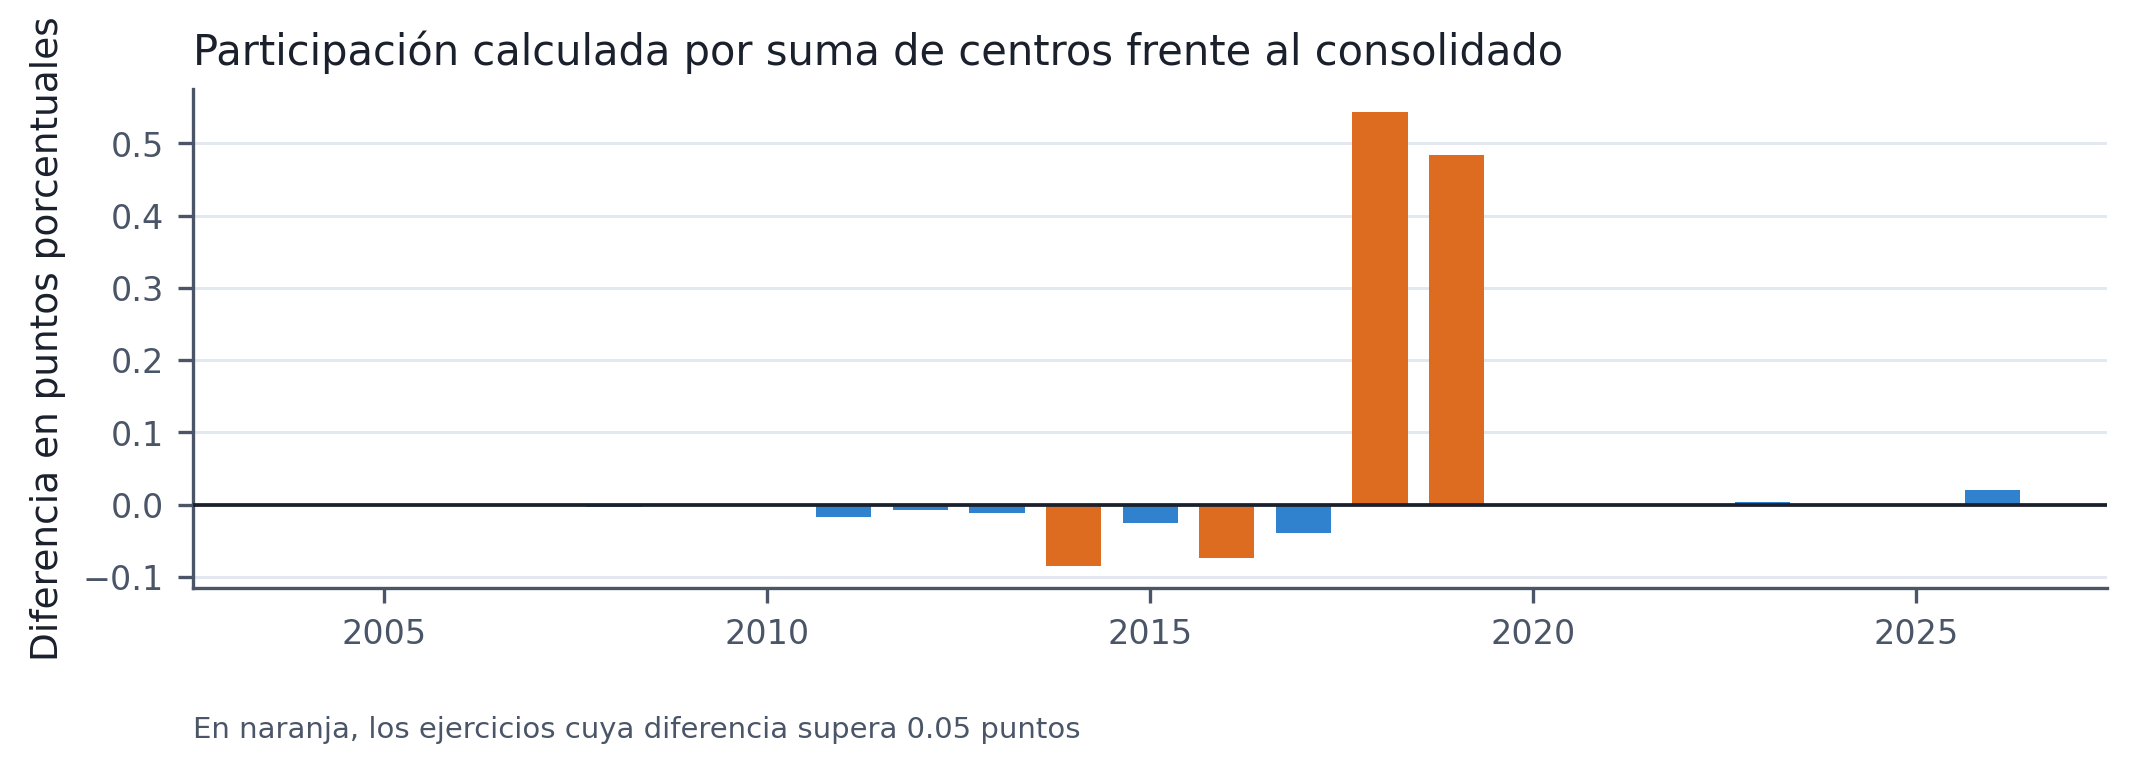
\includegraphics[width=\linewidth]{figuras/figura_4_1.png}\end{center}

\figura{4.1}{Participación calculada por suma de centros frente al consolidado}

\emph{Nota.} Elaboración propia. En naranja los ejercicios cuya diferencia supera 0.05 puntos porcentuales.

La figura contrasta la participación calculada por suma de centros con la calculada sobre el consolidado del proveedor, y destaca los ejercicios en que ambas difieren más de 0.05 puntos porcentuales. Las dos construcciones se superponen durante casi todo el periodo y se separan de manera visible únicamente en 2018 y 2019. Esa separación coincide con el primer año y medio de operación simultánea de las dos bolsas, lo que apunta a un problema de atribución del importe entre centros durante la transición y no a un defecto general de la fuente. La lectura relevante es que la decisión de construir el importe por suma de centros, adoptada en el apartado 3.3.1, no introduce una diferencia material frente al agregado del proveedor salvo en esos dos ejercicios.

La comparación externa coteja el agregado anual con los boletines de la Asociación Mexicana de Instituciones Bursátiles. La razón entre la serie construida y la de esa fuente tiene mediana de 0.4985 en el segmento local y de 0.5149 en el internacional. Al multiplicar por dos, la razón del segmento local pasa a 0.997.

Esos boletines no documentan la convención de conteo que emplean. La razón observada es compatible con que esa fuente sume compras y ventas, de modo que cada operación quede contabilizada dos veces, pero esto es una inferencia a partir de la medición y no una afirmación de la fuente. Si la inferencia es correcta, el factor no afecta la participación, porque es un cociente en el que se cancela, ni las tasas de crecimiento, por la misma razón. Sí impide comparar niveles entre fuentes, y por eso las cifras de nivel de esta investigación no son directamente comparables con las que publica esa asociación, y esa serie se usa solo como contraste externo y no como insumo de ningún resultado.

La razón se mantiene estable entre 2011 y 2024. Se aparta en los ejercicios iniciales y en 2025, donde alcanza 1.186 al multiplicar por dos. El boletín correspondiente a 2025 es el más reciente disponible y podría estar sujeto a revisión, posibilidad que no se verifica aquí y que se deja señalada.

\subseccion{4.1.5 Cobertura histórica y comportamiento de los campos}

La revisión de cobertura identificó un cambio en el tratamiento que la fuente aplica a las sesiones sin operación. La tabla 4.2 reporta, para cada ejercicio, qué proporción de las sesiones sin operación trae de todos modos valor en dos campos de precio.

\tabla{4.2}{Proporción de sesiones sin operación con valor en campos de precio}

{\small
\begin{longtable}[]{@{}
  >{\raggedright\arraybackslash}p{(\linewidth - 8\tabcolsep) * \real{0.2000}}
  >{\raggedright\arraybackslash}p{(\linewidth - 8\tabcolsep) * \real{0.2000}}
  >{\raggedright\arraybackslash}p{(\linewidth - 8\tabcolsep) * \real{0.1999}}
  >{\raggedright\arraybackslash}p{(\linewidth - 8\tabcolsep) * \real{0.2000}}
  >{\raggedright\arraybackslash}p{(\linewidth - 8\tabcolsep) * \real{0.2001}}@{}}
\toprule\noalign{}
\begin{minipage}[b]{\linewidth}\raggedright
\textbf{Ejercicio}
\end{minipage} & \begin{minipage}[b]{\linewidth}\raggedright
\textbf{Sesiones sin operación}
\end{minipage} & \begin{minipage}[b]{\linewidth}\raggedright
\textbf{Precio de cierre}
\end{minipage} & \begin{minipage}[b]{\linewidth}\raggedright
\textbf{Postura de compra}
\end{minipage} & \begin{minipage}[b]{\linewidth}\raggedright
\textbf{Índice de rendimiento total}
\end{minipage} \\
\midrule\noalign{}
\endhead
\bottomrule\noalign{}
\endlastfoot
2004 & 23,146 & 0.1\% & 37.0\% & 0.1\% \\
2010 & 29,658 & 0.0\% & 21.4\% & 0.0\% \\
2018 & 22,237 & 0.0\% & 16.4\% & 0.0\% \\
2019 & 24,289 & 55.5\% & 14.5\% & 55.5\% \\
2020 & 22,780 & 66.9\% & 12.8\% & 66.9\% \\
2026 & 17,300 & 60.0\% & 10.9\% & 60.0\% \\
\end{longtable}
}

\emph{Nota.} Elaboración propia. El ejercicio 2026 cubre de enero a septiembre.

El salto es abrupto y ocurre entre 2018 y 2019, sin transición. Entre 2004 y 2018 el precio de cierre aparece en menos de 0.1\% de las sesiones sin operación, y desde 2019 aparece en más de la mitad. Lo mismo ocurre con el índice de rendimiento total, que es el campo con el que se construyen los rendimientos.

A partir de 2019 la fuente arrastra el último precio conocido a las sesiones en que el instrumento no se negoció, en lugar de dejar el campo vacío. Es un cambio en la práctica del proveedor y no en el comportamiento del mercado.

Un indicador que identificara la sesión sin operación por la ausencia del índice de rendimiento total registraría en 2019 un salto de la proporción de rendimientos cero de alrededor de cincuenta y cinco puntos porcentuales, atribuible al proveedor y no al mercado. Ese es el motivo por el que la ecuación 8 identifica la sesión sin operación mediante el importe operado, que no presenta ese comportamiento. La postura de compra, por su parte, arrastra entre 8\% y 37\% de las sesiones sin operación durante todo el periodo, lo que confirma que ningún campo de precio sirve para establecer si hubo negociación.

\subseccion{4.1.6 Efecto de la regla de muestra por indicador}

El capítulo III sostiene que aplicar un mínimo de sesiones operadas a los cuatro indicadores por igual expulsaría del cálculo a las emisoras menos negociadas, que son precisamente las de mayor proporción de rendimientos cero. La magnitud de ese efecto se midió comparando la mediana anual de la proporción de rendimientos cero con y sin ese mínimo.

La diferencia tiene mediana de 14.41 puntos porcentuales y varía entre 1.01 y 47.29 puntos según el ejercicio. El criterio de Amihud (2002), que exige más de 200 sesiones al año, reduce la muestra de 2,340 a 1,592 observaciones y de 188 a 147 empresas, y con él la mediana del diferencial baja de 1.15\% a 0.70\%.

El sesgo no es constante, y es mayor en los años con más emisoras poco negociadas, que son los iniciales. Un mínimo uniforme habría producido por tanto una serie con pendiente artificial, en la dirección de hacer parecer que la liquidez mejoró más de lo que mejoró. La regla diferenciada por indicador evita ese efecto, y su costo es que los cuatro indicadores no se calculan sobre exactamente la misma muestra, lo que el apartado 4.2 cuantifica.

\subseccion{4.1.7 Estimadores indirectos del diferencial}

Los estimadores de Corwin y Schultz (2012) y de Abdi y Ranaldo (2017) se contrastaron contra el diferencial cotizado observado. Cada uno se calculó conforme a su artículo. El primero incorpora el ajuste por la variación del precio entre el cierre y la apertura, y su valor del periodo es el promedio de los diferenciales de todos los pares de sesiones consecutivas. El segundo promedia el producto dentro del periodo y toma la raíz después, que es el orden que establece su formulación.

\tabla{4.3}{Contraste de los estimadores indirectos}

{\small
\begin{longtable}[]{@{}
  >{\raggedright\arraybackslash}p{(\linewidth - 12\tabcolsep) * \real{0.1316}}
  >{\raggedright\arraybackslash}p{(\linewidth - 12\tabcolsep) * \real{0.1734}}
  >{\raggedright\arraybackslash}p{(\linewidth - 12\tabcolsep) * \real{0.1465}}
  >{\raggedright\arraybackslash}p{(\linewidth - 12\tabcolsep) * \real{0.1465}}
  >{\raggedright\arraybackslash}p{(\linewidth - 12\tabcolsep) * \real{0.1465}}
  >{\raggedright\arraybackslash}p{(\linewidth - 12\tabcolsep) * \real{0.1264}}
  >{\raggedright\arraybackslash}p{(\linewidth - 12\tabcolsep) * \real{0.1291}}@{}}
\toprule\noalign{}
\begin{minipage}[b]{\linewidth}\raggedright
\textbf{Estimador}
\end{minipage} & \begin{minipage}[b]{\linewidth}\raggedright
\textbf{Observaciones}
\end{minipage} & \begin{minipage}[b]{\linewidth}\raggedright
\textbf{Correlación diaria}
\end{minipage} & \begin{minipage}[b]{\linewidth}\raggedright
\textbf{Correlación de rangos diaria}
\end{minipage} & \begin{minipage}[b]{\linewidth}\raggedright
\textbf{Correlación de rangos mensual}
\end{minipage} & \begin{minipage}[b]{\linewidth}\raggedright
\textbf{Mediana mensual del estimador}
\end{minipage} & \begin{minipage}[b]{\linewidth}\raggedright
\textbf{Mediana mensual del observado}
\end{minipage} \\
\midrule\noalign{}
\endhead
\bottomrule\noalign{}
\endlastfoot
Corwin y Schultz & 465,765 & $-$0.0414 & $-$0.0872 & $-$0.3433 & 0.0010 & 0.0106 \\
Abdi y Ranaldo & 465,887 & 0.0198 & $-$0.0684 & $-$0.0834 & 0.0033 & 0.0106 \\
\end{longtable}
}

\emph{Nota.} Elaboración propia.

Ambos estimadores pretenden aproximar el mismo concepto que el diferencial cotizado, de modo que su correlación con él debería ser positiva y alta. Ninguna de las seis correlaciones lo es. La de rangos resulta negativa en los cuatro casos, y en la frecuencia mensual del estimador de Corwin y Schultz alcanza $-$0.3433, lo que significa que ordena las observaciones en sentido contrario al del diferencial observado. Las medianas también difieren en un orden de magnitud.

La causa está en la información que los dos estimadores pueden aprovechar. Ambos derivan el diferencial del rango de precios de la sesión, y en 20.12\% de las sesiones operadas del universo el precio máximo coincide con el mínimo, condición concentrada en las emisoras menos negociadas. En esas sesiones el rango no aporta información sobre el diferencial, de modo que el estimador devuelve cero o queda dependiendo de las sesiones vecinas. La proporción de observaciones sin estimación válida, es decir, aquellas en que el estimador no arroja valor alguno, alcanza 5.25\% en el de Corwin y Schultz y 5.23\% en el de Abdi y Ranaldo.

Esas dos proporciones, junto con las correlaciones bajas y negativas frente al diferencial cotizado, sustentan su exclusión como medidas de liquidez de este trabajo. El resultado no invalida esos estimadores, que fueron construidos para mercados con negociación continua, sino que documenta su límite en un mercado donde una de cada cinco sesiones operadas transcurre a un solo precio. El de Roll (1984) queda indefinido cuando la covarianza serial resulta positiva, situación frecuente en series con negociación esporádica, por lo que tampoco se emplea.

Una última comprobación corresponde a la proporción de rendimientos cero. Lesmond (2005) descarta las sesiones en que el rendimiento es cero para todas las emisoras del mercado, porque un cero simultáneo apunta a la fuente y no a la iliquidez de cada emisora. La regla se aplicó y no encontró nada que descartar. En las 5,727 sesiones con rendimiento medible, la proporción de emisoras con rendimiento cero tiene mediana de 10.84\%, percentil 99 de 35.42\% y máximo de 41.00\%, con 81 emisoras por sesión en la mediana, de modo que ninguna sesión se acerca al cero generalizado. El alcance del filtro de 50\% sobre los rendimientos, que aquí sigue la formulación de Lesmond (2005) sobre precios y no la de Levine y Schmukler (2006) restringida al cociente de Amihud, elimina 132 rendimientos de los 465,486 medibles, que son 0.028\% del total.

\seccion{4.2 El universo y la muestra}

El universo de liquidez comprende 349 series accionarias, de las cuales 323 registran al menos una observación en el periodo. Esas 323 series corresponden a 214 empresas distintas, identificadas con el identificador de empresa de la fuente y no con la raíz de la clave de pizarra.

La diferencia entre ambos criterios es considerable. Agrupar por raíz de ticker habría producido 260 empresas, es decir, cuarenta y seis más de las que existen. Casos como el de Grupo Televisa, con ocho clases accionarias, o los de Coca-Cola FEMSA, CEMEX, Teléfonos de México y Kimberly-Clark de México, con tres o cuatro cada uno, habrían contado como emisoras independientes. Esa diferencia importa porque la clasificación por tamaño se construye sobre la empresa, de modo que contar una empresa varias veces habría alterado los terciles de capitalización y con ellos el contraste de la segunda hipótesis.

El panel anual comprende 2,860 observaciones de empresa y ejercicio, correspondientes a 204 empresas. El número de empresas con información varía entre 115 y 132 según el ejercicio, lo que refleja la entrada y salida de emisoras durante el periodo y no una limitación de la fuente.

\tabla{4.4}{Observaciones válidas por indicador}

{\small
\begin{longtable}[]{@{}
  >{\raggedright\arraybackslash}p{(\linewidth - 4\tabcolsep) * \real{0.3334}}
  >{\raggedright\arraybackslash}p{(\linewidth - 4\tabcolsep) * \real{0.3334}}
  >{\raggedright\arraybackslash}p{(\linewidth - 4\tabcolsep) * \real{0.3333}}@{}}
\toprule\noalign{}
\begin{minipage}[b]{\linewidth}\raggedright
\textbf{Indicador}
\end{minipage} & \begin{minipage}[b]{\linewidth}\raggedright
\textbf{Observaciones válidas}
\end{minipage} & \begin{minipage}[b]{\linewidth}\raggedright
\textbf{Proporción del panel}
\end{minipage} \\
\midrule\noalign{}
\endhead
\bottomrule\noalign{}
\endlastfoot
Diferencial cotizado & 2,340 & 81.8\% \\
Iliquidez de Amihud & 2,321 & 81.2\% \\
Proporción de rendimientos cero & 2,843 & 99.4\% \\
Rotación & 2,824 & 98.7\% \\
\end{longtable}
}

\emph{Nota.} Elaboración propia sobre un panel de 2,860 observaciones.

La tabla muestra el efecto de la regla de muestra por indicador. Los dos indicadores que exigen sesiones operadas cubren alrededor de 82\% del panel, mientras que los dos que se calculan sobre sesiones de vigencia cubren casi la totalidad. La diferencia de dieciocho puntos corresponde a las observaciones de empresa y ejercicio en que la emisora estuvo vigente pero no negoció lo suficiente. Esas observaciones no se pierden, aparecen en los indicadores que sí las admiten, y por eso el deterioro de una emisora que deja de negociarse queda registrado en los rendimientos cero y en la rotación en lugar de desaparecer de la muestra.

\begin{center}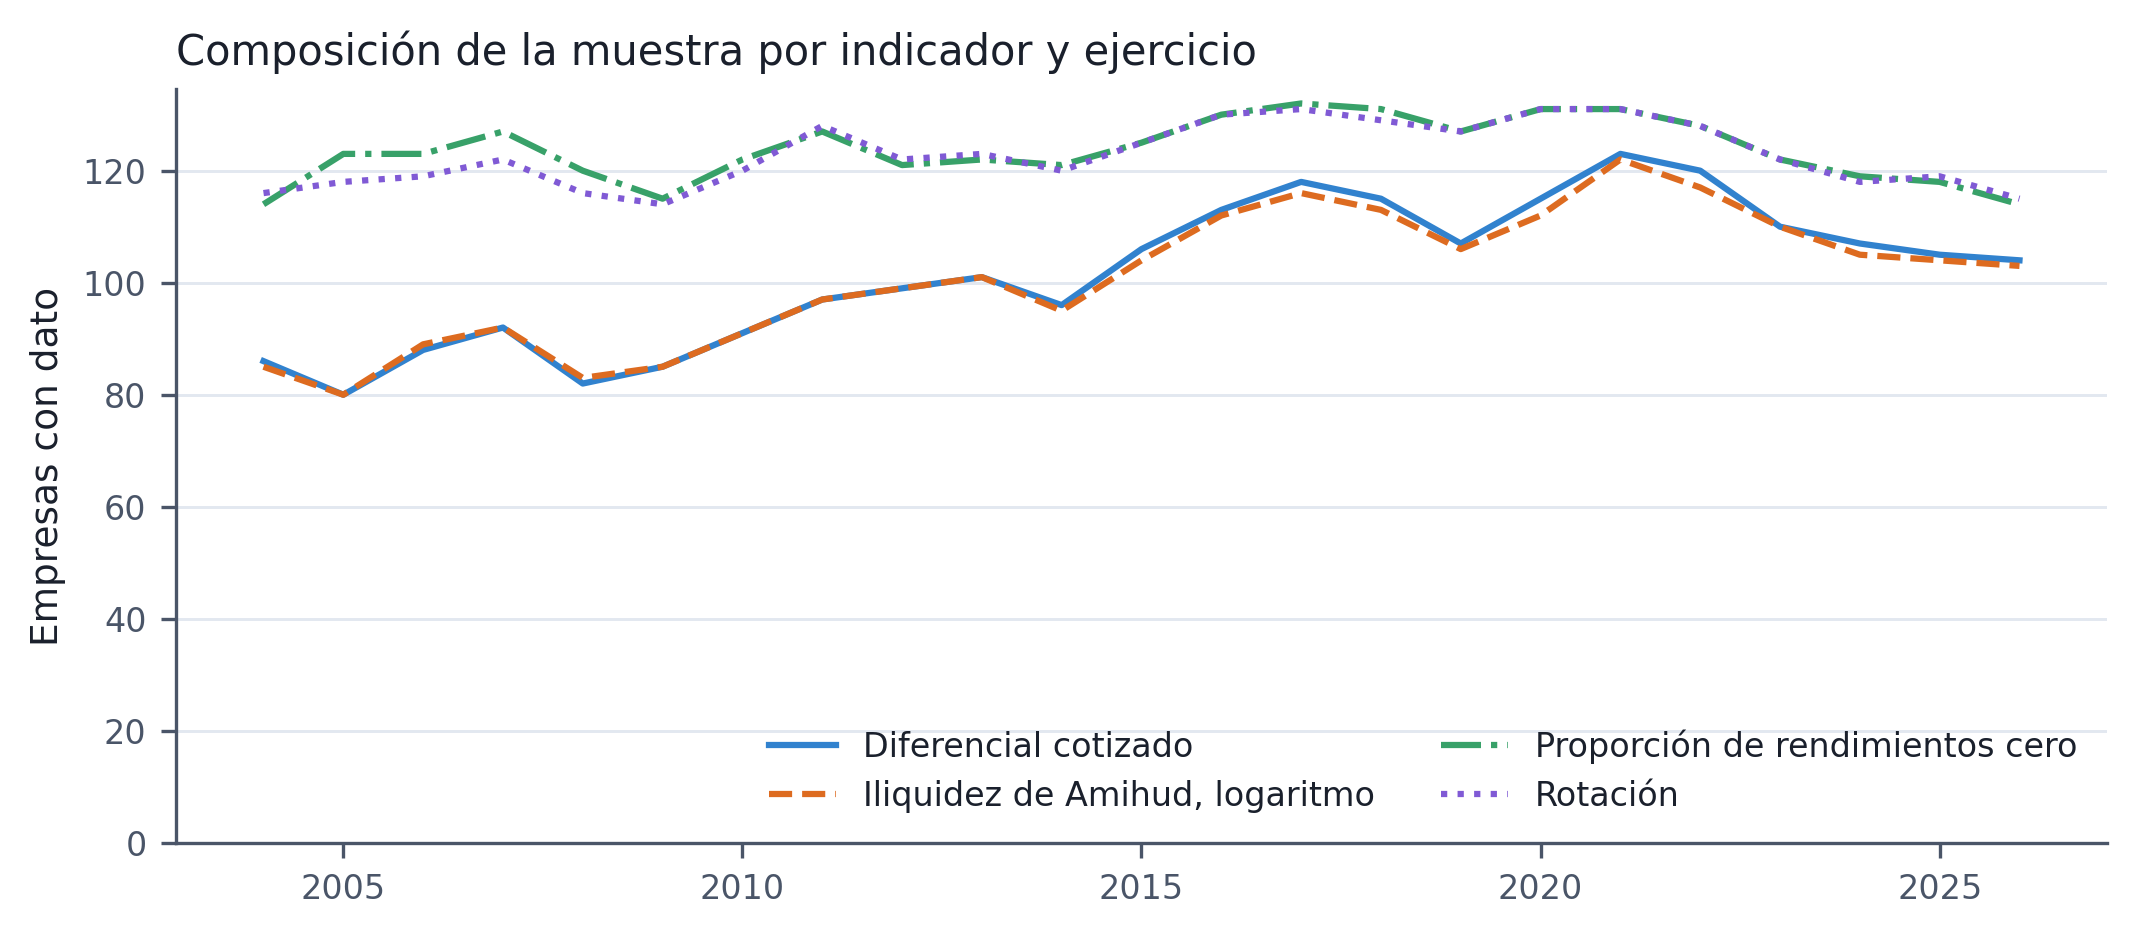
\includegraphics[width=\linewidth]{figuras/figura_4_2.png}\end{center}

\figura{4.2}{Composición de la muestra por indicador y ejercicio}

\emph{Nota.} Elaboración propia. Número de empresas con dato válido en cada indicador.

Las dos líneas superiores, que corresponden a los rendimientos cero y a la rotación, se mantienen casi pegadas al total de empresas vigentes en todos los ejercicios. Las dos inferiores, del diferencial y de la iliquidez, quedan por debajo y se acercan a las primeras con el paso del tiempo. Esa convergencia indica que la proporción de emisoras que alcanzan el mínimo de sesiones operadas aumentó, es decir, que la negociación se volvió menos esporádica en el conjunto del mercado. La separación entre los dos pares de líneas es la parte del mercado que solo puede retratarse con indicadores sin mínimo de operación.

El universo quedó compuesto por 307 acciones ordinarias y 16 certificados de participación, sin fondos cotizados, fideicomisos de bienes raíces ni recibos de depósito. En cuanto a su estado, 104 series permanecen activas y 219 corresponden a instrumentos deslistados, adquiridos, suspendidos o liquidados.

Esa composición es la que permite evitar el sesgo de supervivencia, que consiste en estudiar solo a las empresas que llegaron hasta el final del periodo. Sin las 219 series inactivas, los ejercicios iniciales quedarían poblados únicamente por emisoras que sobrevivieron veintidós años, es decir, por las más grandes y mejor negociadas, y la liquidez de 2004 aparecería mucho mejor de lo que fue. El deterioro posterior que documenta el apartado 4.4 quedaría en parte oculto por esa selección.

La clasificación de sector no pudo obtenerse para todas las empresas. La fuente la reporta para 163 de las 323 series y no la mantiene para las emisoras que dejaron de cotizar, de modo que las descripciones por sector quedan fuera de este capítulo y la caracterización de la muestra se hace por tercil de capitalización, que sí está disponible para la totalidad.

\seccion{4.3 Primera hipótesis. Evolución de la participación del SIC}

\subseccion{4.3.1 Trayectoria de la participación}

La participación del Sistema Internacional de Cotizaciones en el importe operado total pasó de 3.13\% en 2004 a 45.83\% en 2026, con un máximo de 55.91\% en 2020. La figura 4.3 presenta la serie mensual.

\begin{center}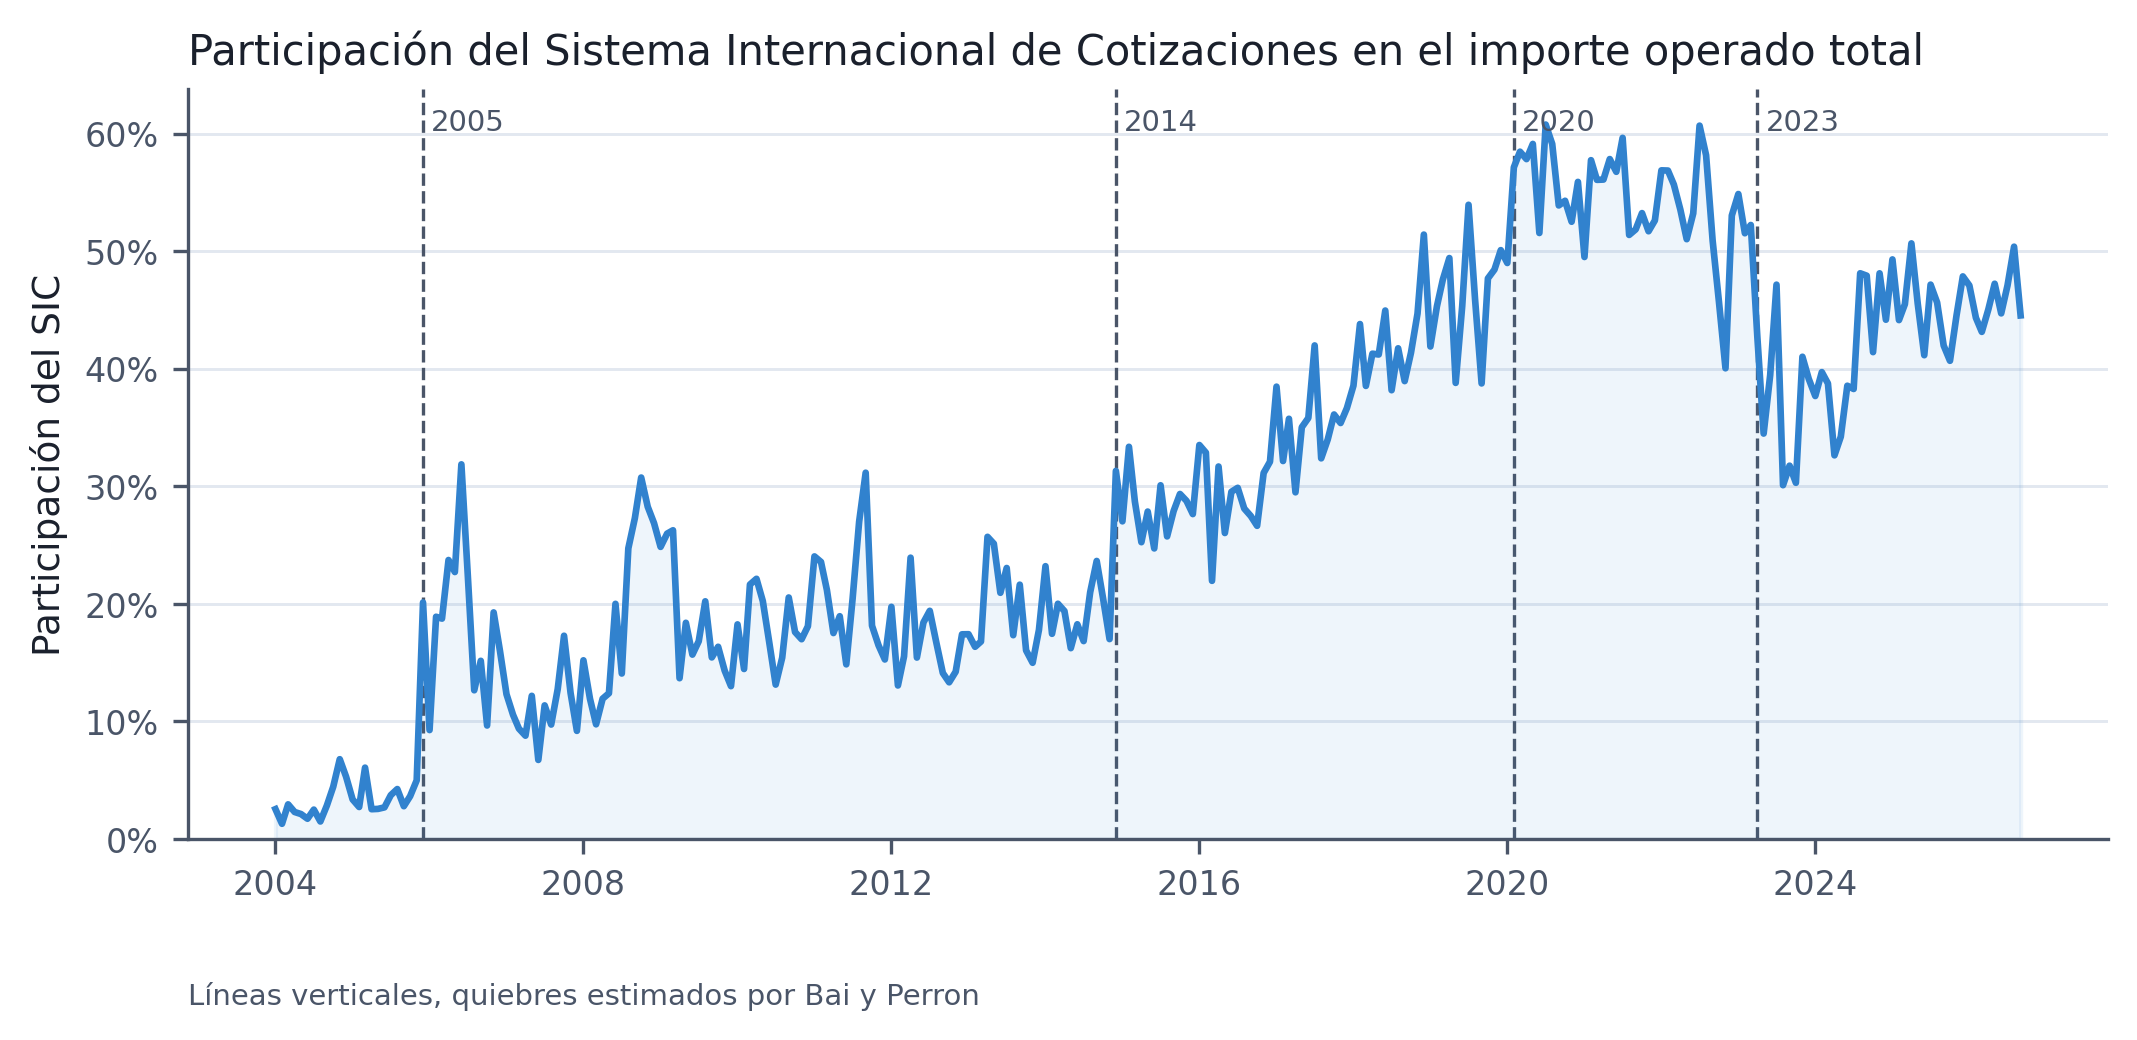
\includegraphics[width=\linewidth]{figuras/figura_4_3.png}\end{center}

\figura{4.3}{Participación del SIC en el importe operado total}

\emph{Nota.} Elaboración propia. Las líneas verticales señalan los quiebres estimados por Bai y Perron (1998).

La trayectoria no es monótona y conviene leerla en cuatro etapas. Crece con rapidez hasta 2006, se estabiliza alrededor de 18\% a 21\% durante casi una década, acelera a partir de 2015, alcanza su máximo entre 2020 y 2022, cuando el segmento internacional supera al local, y desciende después hasta estabilizarse en torno a 42\% a 46\%. Las líneas verticales no coinciden con el inicio de operaciones de la segunda bolsa, un punto al que el apartado 4.3.2 vuelve.

\tabla{4.5}{Participación del SIC por ejercicio}

{\small
\begin{longtable}[]{@{}
  >{\raggedright\arraybackslash}p{(\linewidth - 10\tabcolsep) * \real{0.1632}}
  >{\raggedright\arraybackslash}p{(\linewidth - 10\tabcolsep) * \real{0.1701}}
  >{\raggedright\arraybackslash}p{(\linewidth - 10\tabcolsep) * \real{0.1633}}
  >{\raggedright\arraybackslash}p{(\linewidth - 10\tabcolsep) * \real{0.1701}}
  >{\raggedright\arraybackslash}p{(\linewidth - 10\tabcolsep) * \real{0.1633}}
  >{\raggedright\arraybackslash}p{(\linewidth - 10\tabcolsep) * \real{0.1701}}@{}}
\toprule\noalign{}
\begin{minipage}[b]{\linewidth}\raggedright
\textbf{Ejercicio}
\end{minipage} & \begin{minipage}[b]{\linewidth}\raggedright
\textbf{Participación}
\end{minipage} & \begin{minipage}[b]{\linewidth}\raggedright
\textbf{Ejercicio}
\end{minipage} & \begin{minipage}[b]{\linewidth}\raggedright
\textbf{Participación}
\end{minipage} & \begin{minipage}[b]{\linewidth}\raggedright
\textbf{Ejercicio}
\end{minipage} & \begin{minipage}[b]{\linewidth}\raggedright
\textbf{Participación}
\end{minipage} \\
\midrule\noalign{}
\endhead
\bottomrule\noalign{}
\endlastfoot
2004 & 3.13\% & 2012 & 16.49\% & 2020 & 55.91\% \\
2005 & 5.11\% & 2013 & 19.69\% & 2021 & 54.68\% \\
2006 & 18.71\% & 2014 & 20.72\% & 2022 & 53.24\% \\
2007 & 11.34\% & 2015 & 28.07\% & 2023 & 41.79\% \\
2008 & 19.19\% & 2016 & 29.27\% & 2024 & 41.09\% \\
2009 & 17.85\% & 2017 & 35.56\% & 2025 & 45.34\% \\
2010 & 18.09\% & 2018 & 42.16\% & 2026 & 45.83\% \\
2011 & 21.18\% & 2019 & 46.11\% & & \\
\end{longtable}
}

\emph{Nota.} Elaboración propia. El ejercicio 2026 cubre de enero a septiembre.

En 2004 poco más de tres de cada cien pesos operados en el mercado accionario mexicano correspondían a valores extranjeros listados en el país. Para 2020 eran casi cincuenta y seis de cada cien, es decir, el segmento internacional llegó a mover más dinero que el conjunto de las emisoras mexicanas. Ese es el hecho que da sentido a la pregunta de investigación.

\subseccion{4.3.2 Tendencia y quiebres}

La regresión de la participación mensual contra el tiempo, con errores robustos a heterocedasticidad y autocorrelación y un rezago de truncamiento de cinco periodos, arroja una pendiente de 0.1811 puntos porcentuales por mes, con error estándar de 0.0133 y estadístico t de 13.61. El coeficiente de determinación es 0.7681 sobre 273 observaciones mensuales.

La pendiente indica que, en promedio, la participación subió algo más de dos puntos porcentuales por año a lo largo del periodo. El error estándar mide con cuánta precisión está estimada esa pendiente, y el estadístico t es el cociente entre ambos, de modo que un valor de 13.61 indica que la pendiente es trece veces mayor que su propia imprecisión. El valor p es la probabilidad de observar un resultado así de extremo si en realidad no existiera tendencia alguna, y aquí es menor a 0.001. Conviene leerlo con cuidado, porque un valor p pequeño indica que el resultado es poco compatible con la ausencia de tendencia, no que la tendencia tenga 99.9\% de probabilidad de ser cierta. El coeficiente de determinación de 0.7681 indica que el paso del tiempo da cuenta de alrededor de 77\% de la variación de la serie mensual.

La prueba de Mann y Kendall confirma el resultado sin suponer forma funcional, con tau de 0.683 y probabilidad menor a 0.001. El coeficiente tau mide la dirección y la consistencia de una tendencia, en una escala de $-$1 a +1, comparando cada par de meses de la serie y contando en cuántos la participación subió y en cuántos bajó. Un valor de 0.683 indica que los aumentos fueron bastante más frecuentes que los descensos, y no un aumento de 68.3\%. La ventaja de esta prueba es que no exige que la tendencia sea una línea recta, de modo que su coincidencia con la regresión refuerza el resultado.

Las pruebas de raíz unitaria no permiten descartarla. La de Dickey y Fuller arroja una probabilidad de 0.4671, de modo que no se rechaza la presencia de raíz unitaria, y la de Kwiatkowski y otros arroja 0.01, de modo que sí se rechaza la estacionariedad. Una serie con raíz unitaria es una serie cuyo nivel no tiende a regresar a un promedio, de modo que las desviaciones se acumulan en lugar de corregirse. Ambas pruebas apuntan en la misma dirección, y por esa razón la inferencia de la tercera hipótesis se apoya también en la estimación en primeras diferencias, es decir, en el cambio mensual de cada variable y no en su nivel.

El procedimiento de Bai y Perron estima cuatro quiebres dentro del máximo de cuatro que se le especificó, en diciembre de 2005, diciembre de 2014, febrero de 2020 y abril de 2023. Un quiebre estructural es un cambio identificable en el comportamiento de la serie, es decir, un punto a partir del cual su nivel o su pendiente dejan de ser los mismos. Las pruebas de Chow sobre las fechas que la cronología documenta rechazan la ausencia de quiebre en ambas, con estadístico F de 5.66 y probabilidad de 0.004 para enero de 2014, y de 81.25 con probabilidad menor a 0.001 para el 25 de julio de 2018. Conviene precisar que la serie es mensual, de modo que el corte no puede situarse dentro de un mes. Con la fecha del 25 de julio de 2018, julio queda del lado anterior y el contraste compara agosto de 2018 en adelante contra los meses previos, que es el primer mes completo de operación simultánea de las dos bolsas.

Los dos procedimientos coinciden parcialmente, y la diferencia es informativa. El quiebre estimado de diciembre de 2014 está próximo a la reforma que modificó las condiciones de acceso al segmento, y el de febrero de 2020 coincide con el inicio de la pandemia. La prueba de Chow establece que el inicio de operaciones de BIVA coincide con un cambio estadísticamente significativo en la trayectoria de la participación, de modo que julio de 2018 es una fecha relevante para describir la transformación del mercado. Que esa fecha no aparezca entre los cuatro quiebres que selecciona Bai y Perron no contradice el resultado, porque las dos pruebas responden preguntas distintas. La de Chow evalúa una fecha elegida de antemano, mientras que la de Bai y Perron escoge fechas conforme a su propio criterio y a la restricción de doce meses por segmento. Los dos resultados en conjunto permiten reconocer julio de 2018 como un punto relevante de la evolución del mercado, sin atribuir a BIVA la totalidad del cambio observado. Como varias de estas fechas están próximas entre sí, la evidencia disponible no permite separar sus efectos.

\subseccion{4.3.3 Crecimiento real de cada segmento}

\tabla{4.6}{Tasas de crecimiento real anual compuesto}

{\small
\begin{longtable}[]{@{}
  >{\raggedright\arraybackslash}p{(\linewidth - 8\tabcolsep) * \real{0.1999}}
  >{\raggedright\arraybackslash}p{(\linewidth - 8\tabcolsep) * \real{0.2001}}
  >{\raggedright\arraybackslash}p{(\linewidth - 8\tabcolsep) * \real{0.2000}}
  >{\raggedright\arraybackslash}p{(\linewidth - 8\tabcolsep) * \real{0.2000}}
  >{\raggedright\arraybackslash}p{(\linewidth - 8\tabcolsep) * \real{0.2000}}@{}}
\toprule\noalign{}
\begin{minipage}[b]{\linewidth}\raggedright
\textbf{Tramo}
\end{minipage} & \begin{minipage}[b]{\linewidth}\raggedright
\textbf{Segmento internacional}
\end{minipage} & \begin{minipage}[b]{\linewidth}\raggedright
\textbf{Segmento local}
\end{minipage} & \begin{minipage}[b]{\linewidth}\raggedright
\textbf{Producto interno bruto}
\end{minipage} & \begin{minipage}[b]{\linewidth}\raggedright
\textbf{Brecha local frente al producto}
\end{minipage} \\
\midrule\noalign{}
\endhead
\bottomrule\noalign{}
\endlastfoot
2004 a 2025 & 21.59\% & 4.17\% & 1.53\% & +2.64 pp \\
2004 a 2013 & 46.69\% & 17.10\% & 1.78\% & +15.33 pp \\
2014 a 2018 & 21.81\% & $-$5.74\% & 2.08\% & $-$7.82 pp \\
2019 a 2025 & 1.04\% & 1.57\% & 0.97\% & +0.59 pp \\
\end{longtable}
}

\emph{Nota.} Elaboración propia. Importes deflactados con el índice nacional de precios al consumidor. El producto real proviene de las cuentas nacionales a precios constantes de 2018, y las tasas de crecimiento de ambas magnitudes se comparan sobre los mismos intervalos. Las dos series tienen periodos de referencia distintos, de modo que el índice de precios se reexpresa tomando como cien el promedio del año 2018 antes de deflactar.

El crecimiento del segmento internacional se concentró en la primera mitad del periodo. Entre 2004 y 2013 creció 46.69\% real anual, y entre 2019 y 2025 apenas 1.04\%, es decir, prácticamente se detuvo. El segmento local presenta la trayectoria opuesta, puesto que creció con fuerza hasta 2013, se contrajo 5.74\% real anual entre 2014 y 2018, y recuperó un crecimiento modesto de 1.57\% entre 2019 y 2025.

La tasa de crecimiento anual compuesto es la tasa constante que llevaría del valor inicial al final en el número de años del tramo, de modo que resume la trayectoria en una sola cifra y no distingue si el crecimiento fue parejo o concentrado en unos pocos años. Las tasas de los tramos cortos son por tanto más sensibles a los valores de sus extremos que las del periodo completo.

El aumento de participación no proviene de los últimos años. Entre 2019 y 2025 el segmento local creció a una tasa mayor que el internacional, 1.57\% frente a 1.04\%, y la participación del internacional retrocedió dentro de ese tramo, de 46.11\% a 45.34\%. Esto tiene una consecuencia para toda la tesis, porque sitúa el avance del segmento internacional en la primera mitad del periodo y no en el presente, y obliga a contrastar ese momento con el momento en que la liquidez de las emisoras mexicanas se deterioró, que el apartado 4.4 ubica después de 2014.

\begin{center}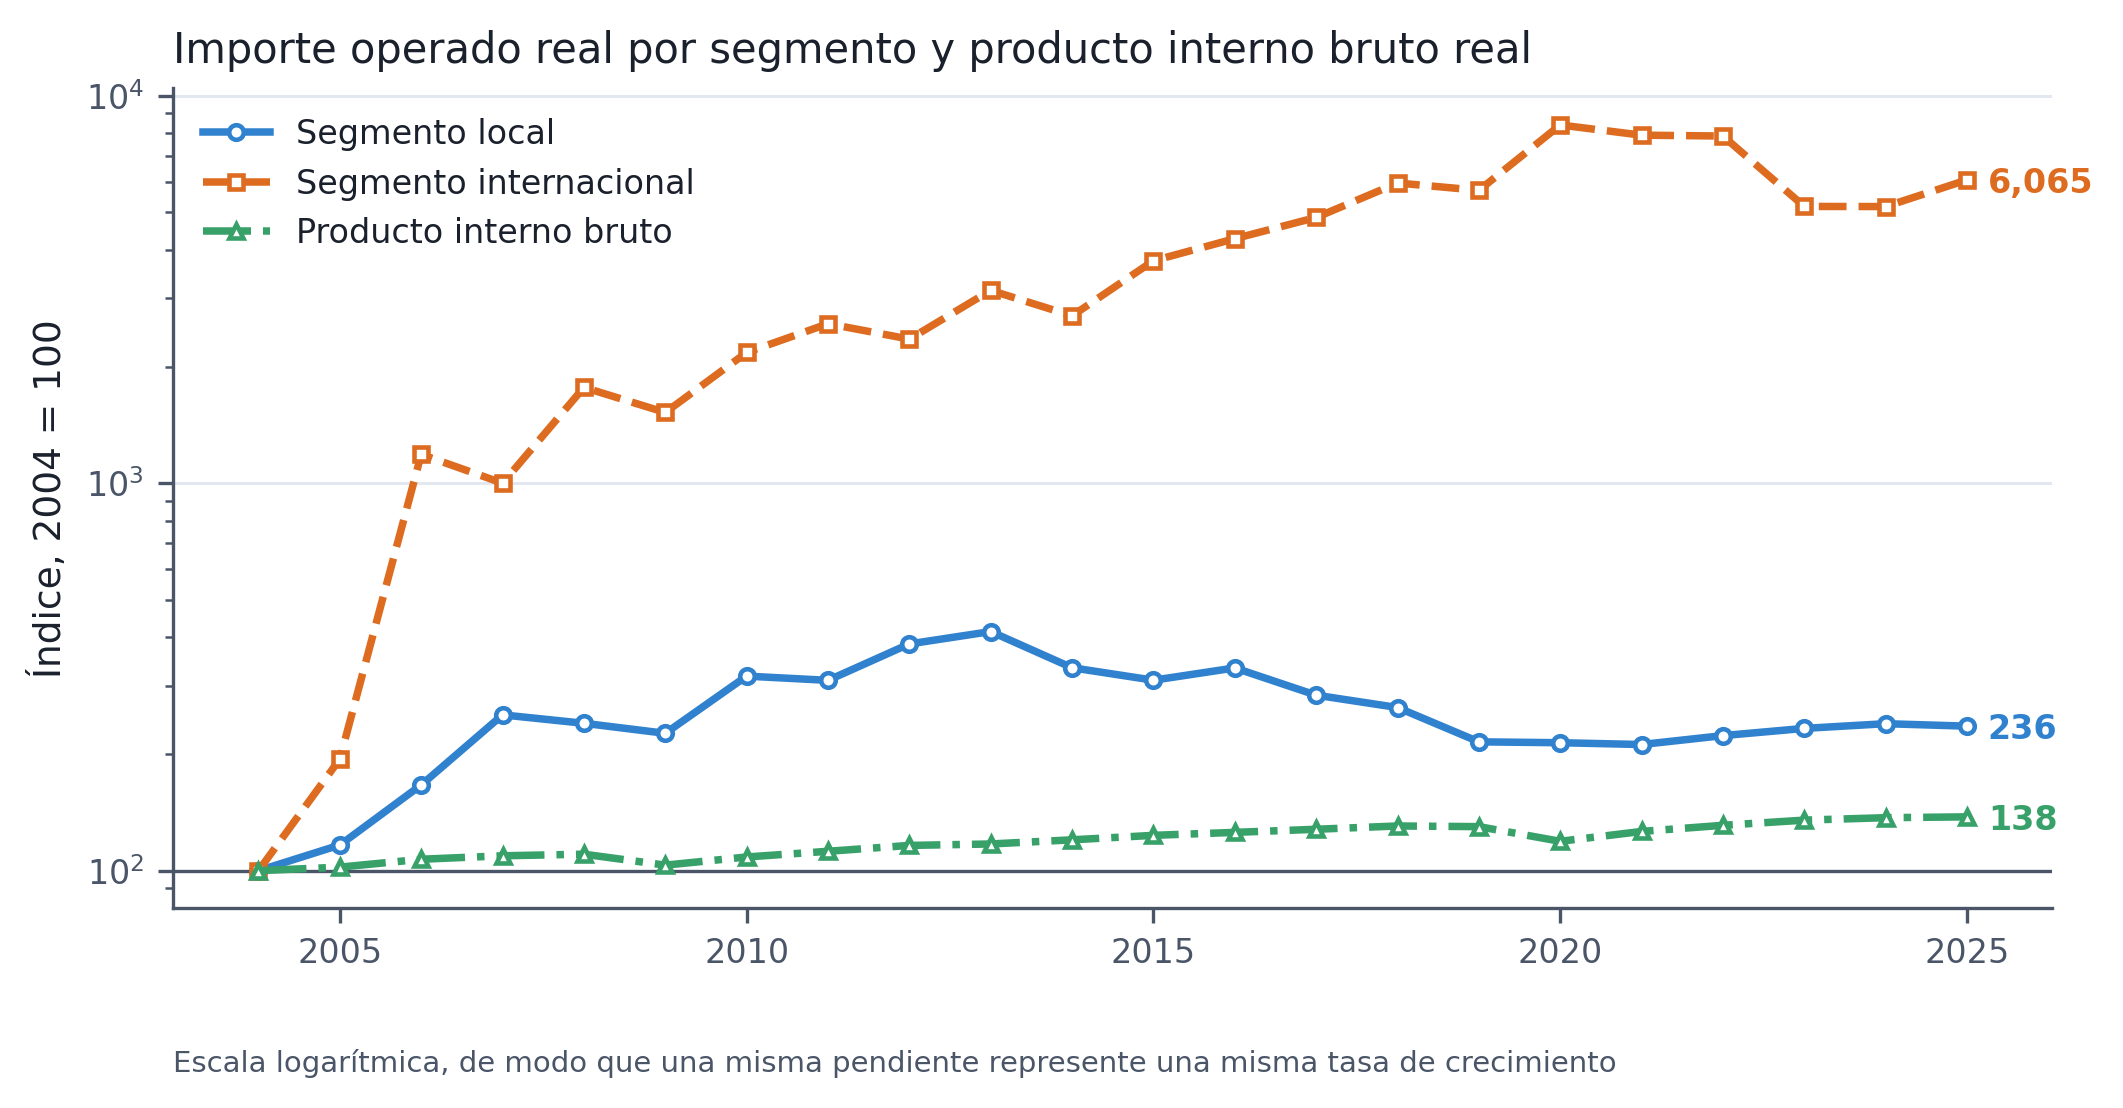
\includegraphics[width=\linewidth]{figuras/figura_4_4.png}\end{center}

\figura{4.4}{Importe operado real por segmento y producto interno bruto real}

\emph{Nota.} Elaboración propia. Índice con base 2004 igual a 100 y escala logarítmica, de modo que una misma pendiente represente una misma tasa de crecimiento.

La escala logarítmica permite comparar tasas y no niveles, de modo que lo que importa es la inclinación de cada línea y no su altura. La del segmento internacional es muy inclinada hasta 2013 y se aplana después, la del local sube, baja y vuelve a subir con poca pendiente, y la del producto avanza de manera casi recta y mucho más plana que las dos anteriores. La imagen deja ver que el mercado accionario, en sus dos segmentos, creció por encima de la economía durante la primera mitad del periodo y dejó de hacerlo en la segunda.

\begin{center}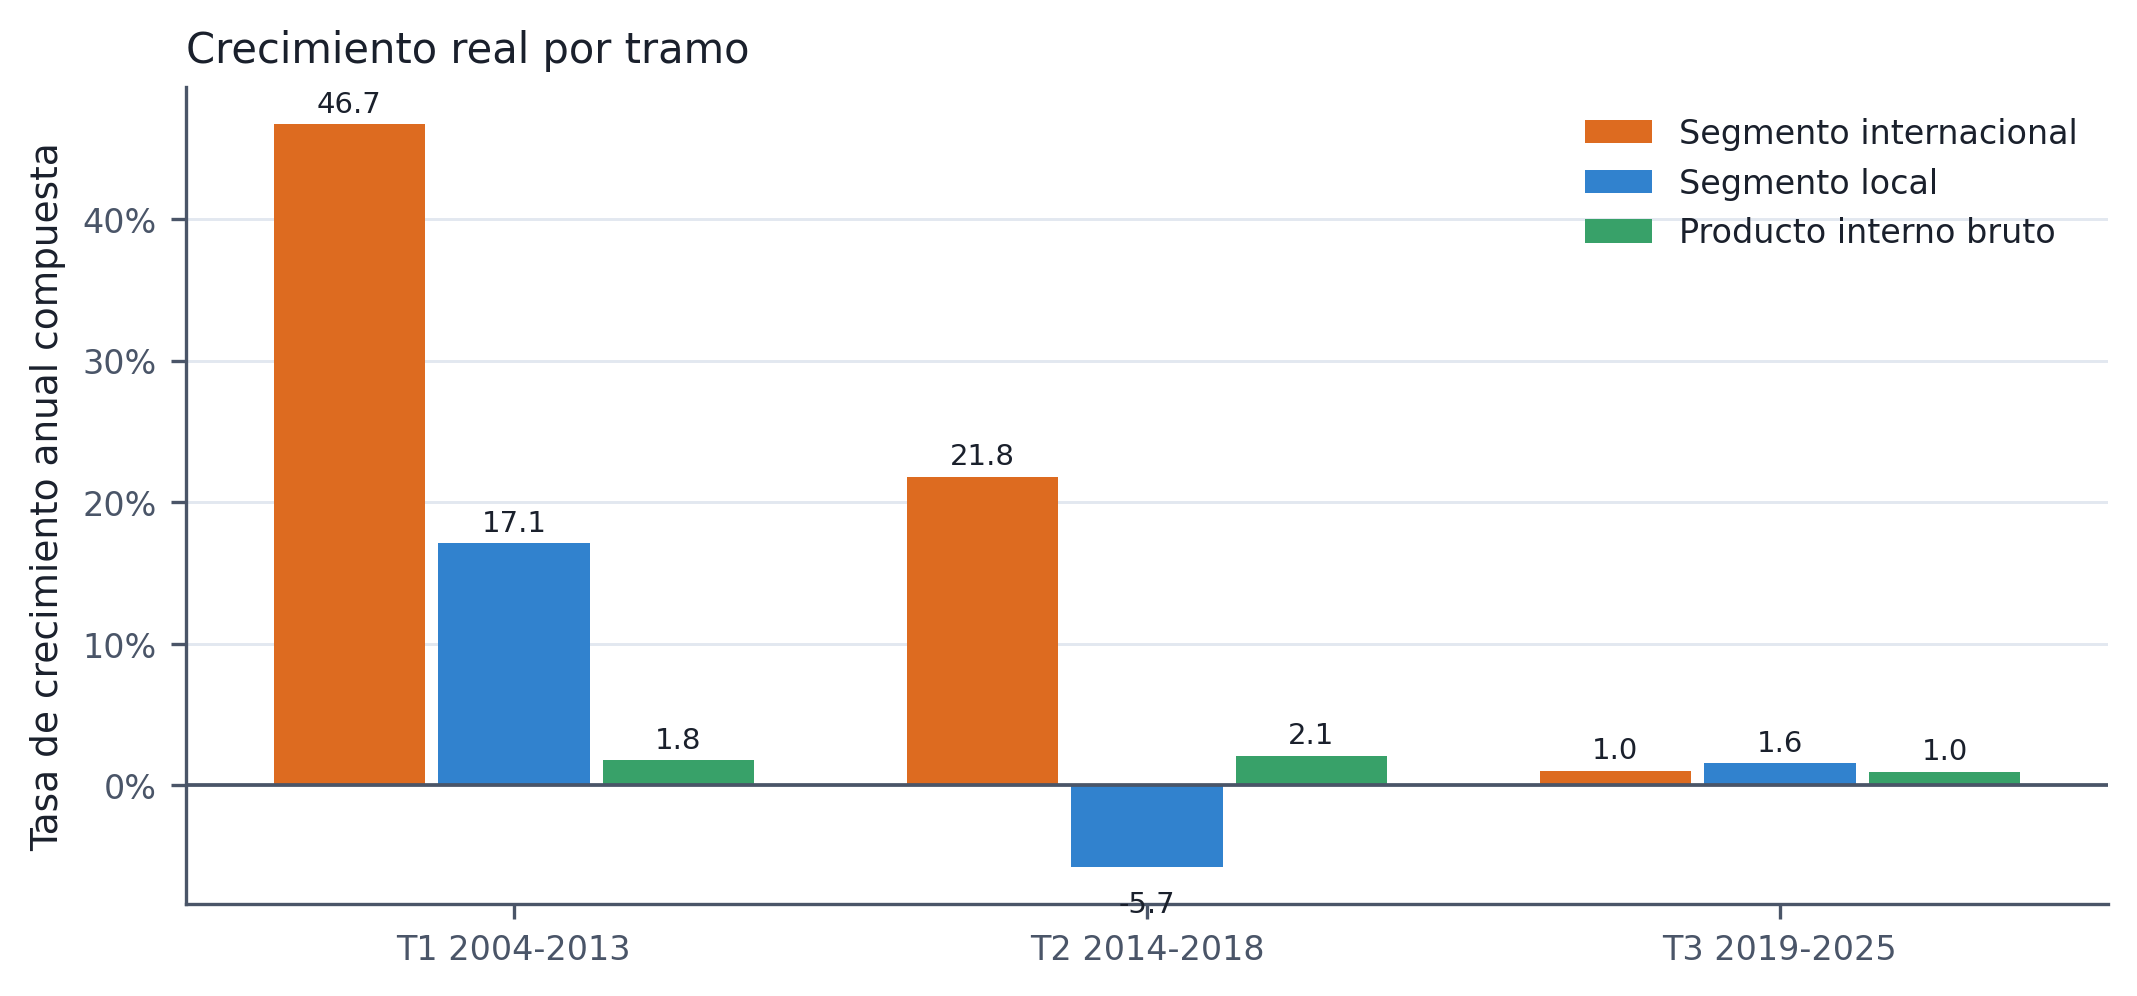
\includegraphics[width=\linewidth]{figuras/figura_4_5.png}\end{center}

\figura{4.5}{Crecimiento real por tramo}

\emph{Nota.} Elaboración propia. Tasa de crecimiento anual compuesta de cada segmento y del producto interno bruto.

Las barras hacen visible el cambio de régimen. En el primer tramo las tres barras son positivas y la del segmento internacional es con diferencia la más alta. En el segundo la del segmento local cruza por debajo de cero, único caso de contracción en todo el periodo. En el tercero las tres barras quedan casi a la misma altura y muy cerca de cero, de modo que los dos segmentos y la economía crecen a tasas parecidas y bajas. El contraste entre el primer tramo y el tercero es el hallazgo central de esta hipótesis.

\subseccion{4.3.4 Lectura de la hipótesis}

\textbf{H1a.} La participación aumentó de 3.13\% a 45.83\%, pero la serie no permite distinguir una tendencia determinista de una caminata aleatoria con deriva. La regresión contra el tiempo del apartado 4.3.2 no es válida si la serie tiene raíz unitaria: con caminatas aleatorias del mismo largo, esa prueba encuentra una tendencia significativa en 82\% de los casos. La prueba válida es la media de las diferencias mensuales del logit de la participación, con errores de Newey--West. La deriva es positiva, de 0.151 por año, y no significativa ($p=0.303$); la más clara corresponde a 2014--2018 (0.318 por año, $p=0.078$), después de la apertura del SIC a cualquier inversionista en enero de 2014. H1a se sostiene como hecho descriptivo y no como tendencia estadística.

\textbf{H1b.} El importe operado real del segmento local sobre el producto interno bruto real, con 2004 igual a 100, llega a 353 en 2013 y baja a 175 en 2024. La tasa entre extremos de la Tabla 4.6 (4.17\% contra 1.59\% del producto) depende del año inicial: con la pendiente logarítmica de todo el periodo el segmento local crece 1.50\%, prácticamente lo mismo que la economía, y desde 2013 se contrae 4.58\% real anual. H1b se sostiene: el segmento local se expandió hasta 2013 y se contrajo frente a la economía desde entonces.

\seccion{4.4 Segunda hipótesis. Evolución de la liquidez y diferencias por tamaño}

\subseccion{4.4.1 Trayectoria de los indicadores}

\tabla{4.7}{Mediana de cada indicador en tres momentos}

{\small
\begin{longtable}[]{@{}
  >{\raggedright\arraybackslash}p{(\linewidth - 6\tabcolsep) * \real{0.2501}}
  >{\raggedright\arraybackslash}p{(\linewidth - 6\tabcolsep) * \real{0.2499}}
  >{\raggedright\arraybackslash}p{(\linewidth - 6\tabcolsep) * \real{0.2501}}
  >{\raggedright\arraybackslash}p{(\linewidth - 6\tabcolsep) * \real{0.2499}}@{}}
\toprule\noalign{}
\begin{minipage}[b]{\linewidth}\raggedright
\textbf{Indicador}
\end{minipage} & \begin{minipage}[b]{\linewidth}\raggedright
\textbf{2004}
\end{minipage} & \begin{minipage}[b]{\linewidth}\raggedright
\textbf{Valor extremo favorable}
\end{minipage} & \begin{minipage}[b]{\linewidth}\raggedright
\textbf{2026}
\end{minipage} \\
\midrule\noalign{}
\endhead
\bottomrule\noalign{}
\endlastfoot
Diferencial cotizado & 2.69\% & 0.45\% en 2014 & 1.54\% \\
Iliquidez de Amihud, logaritmo & $-$2.69 & $-$6.47 en 2014 & $-$3.65 \\
Proporción de rendimientos cero & 72.8\% & 3.8\% en 2018 & 27.4\% \\
Rotación & 8.22\% & 17.35\% en 2013 & 4.39\% en 2025 \\
\end{longtable}
}

\emph{Nota.} Elaboración propia. En los tres primeros indicadores un valor menor indica mejores condiciones, y en la rotación un valor mayor indica mayor actividad. En la rotación la última columna reporta 2025, que es el último ejercicio completo, porque su numerador acumula el importe del periodo y el ejercicio 2026 cubre solo de enero a septiembre. El acumulado de esos nueve meses es de 3.07\%, equivalente a 4.09\% si se lleva a doce meses.

La trayectoria de los tres indicadores de precio tiene forma de U. Mejoran de manera sostenida hasta mediados de la década pasada, alcanzan su mejor nivel entre 2014 y 2018, y se deterioran después. El diferencial cotizado bajó de 2.69\% a 0.45\% y volvió a subir hasta 1.54\%, es decir, se triplicó desde su mínimo. La rotación sigue un perfil distinto, con máximo de 17.35\% en 2013 y descenso posterior hasta 4.39\% en 2025. El ejercicio completo de menor rotación es 2024, con 3.83\%.

El diferencial cotizado de 1.54\% quiere decir que, en la emisora mediana de 2026, la diferencia entre el mejor precio de compra y el mejor precio de venta equivale a poco más de 1.5\% del precio, que es el costo que paga quien necesita comprar o vender de inmediato. Una proporción de rendimientos cero de 27.4\% significa que en algo más de una de cada cuatro sesiones el precio de la emisora mediana no se movió, lo que en la literatura se interpreta como señal de que no llegó información suficiente para mover el precio o no hubo negociación que lo moviera. Una rotación de 4.39\% indica que en el año se operó el equivalente a algo más de 4\% del valor de mercado de la empresa.

Un diferencial que se triplica desde su mínimo y una rotación que cae a una cuarta parte de su máximo describen un mercado donde operar se volvió más costoso y menos frecuente para la emisora mediana. Al mismo tiempo, los niveles de 2026 siguen siendo mejores que los de 2004 en los tres indicadores de precio, de modo que el deterioro reciente no borra la mejora acumulada de las dos primeras décadas. Las dos cosas son ciertas y el apartado 4.4.4 las separa con cuidado.

Esa forma tiene una consecuencia estadística que el diseño anticipó. La prueba de Mann y Kendall busca una tendencia monótona, de modo que una trayectoria que cambia de dirección a la mitad del periodo produce signos que se cancelan.

\tabla{4.8}{Prueba de Mann y Kendall sobre la serie mensual, por tramo}

{\small
\begin{longtable}[]{@{}
  >{\raggedright\arraybackslash}p{(\linewidth - 8\tabcolsep) * \real{0.2000}}
  >{\raggedright\arraybackslash}p{(\linewidth - 8\tabcolsep) * \real{0.2000}}
  >{\raggedright\arraybackslash}p{(\linewidth - 8\tabcolsep) * \real{0.2000}}
  >{\raggedright\arraybackslash}p{(\linewidth - 8\tabcolsep) * \real{0.2000}}
  >{\raggedright\arraybackslash}p{(\linewidth - 8\tabcolsep) * \real{0.2000}}@{}}
\toprule\noalign{}
\begin{minipage}[b]{\linewidth}\raggedright
\textbf{Indicador}
\end{minipage} & \begin{minipage}[b]{\linewidth}\raggedright
\textbf{Periodo completo}
\end{minipage} & \begin{minipage}[b]{\linewidth}\raggedright
\textbf{2004 a 2013}
\end{minipage} & \begin{minipage}[b]{\linewidth}\raggedright
\textbf{2014 a 2018}
\end{minipage} & \begin{minipage}[b]{\linewidth}\raggedright
\textbf{2019 a 2025}
\end{minipage} \\
\midrule\noalign{}
\endhead
\bottomrule\noalign{}
\endlastfoot
Diferencial cotizado & tau $-$0.063, p 0.120 & tau $-$0.629, p \textless{} 0.001 & tau +0.489, p \textless{} 0.001 & tau +0.552, p \textless{} 0.001 \\
Iliquidez de Amihud & tau +0.193, p \textless{} 0.001 & tau $-$0.522, p \textless{} 0.001 & tau +0.441, p \textless{} 0.001 & tau +0.199, p 0.008 \\
Rendimientos cero & tau $-$0.265, p \textless{} 0.001 & tau $-$0.736, p \textless{} 0.001 & tau $-$0.068, p 0.436 & tau +0.571, p \textless{} 0.001 \\
Rotación & tau $-$0.211, p \textless{} 0.001 & tau +0.368, p \textless{} 0.001 & tau $-$0.350, p \textless{} 0.001 & tau $-$0.378, p \textless{} 0.001 \\
\end{longtable}
}

\emph{Nota.} Elaboración propia. Probabilidades ajustadas por el procedimiento de Holm dentro de cada tramo. En los tres primeros indicadores un tau positivo señala deterioro, y en la rotación lo señala un tau negativo. La prueba corrige por empates pero no por autocorrelación temporal, de modo que en series mensuales persistentes sus probabilidades deben leerse como indicativas y no como una medida exacta del error de primer tipo.

El contraste es nítido en el diferencial cotizado. Sobre el periodo completo la prueba no detecta tendencia alguna, con tau de $-$0.063 y probabilidad de 0.120. Dentro de cada tramo detecta tres tendencias fuertes y todas significativas, la primera de mejora y las dos siguientes de deterioro.

Cuando se hacen varias pruebas a la vez aumenta la probabilidad de que alguna resulte significativa por azar. El procedimiento de Holm endurece el criterio en proporción al número de pruebas de la familia, de modo que las probabilidades reportadas ya incorporan ese endurecimiento y pueden leerse directamente contra el umbral de 5\%.

Una sola prueba sobre el periodo completo habría concluido que el diferencial cotizado no cambió en veintidós años, cuando lo que ocurrió fue una mejora marcada seguida de un deterioro igualmente marcado. La decisión de partir el periodo en tramos, tomada en el apartado 3.4.2 antes de ver los resultados, es la que permite ver la trayectoria real.

\begin{center}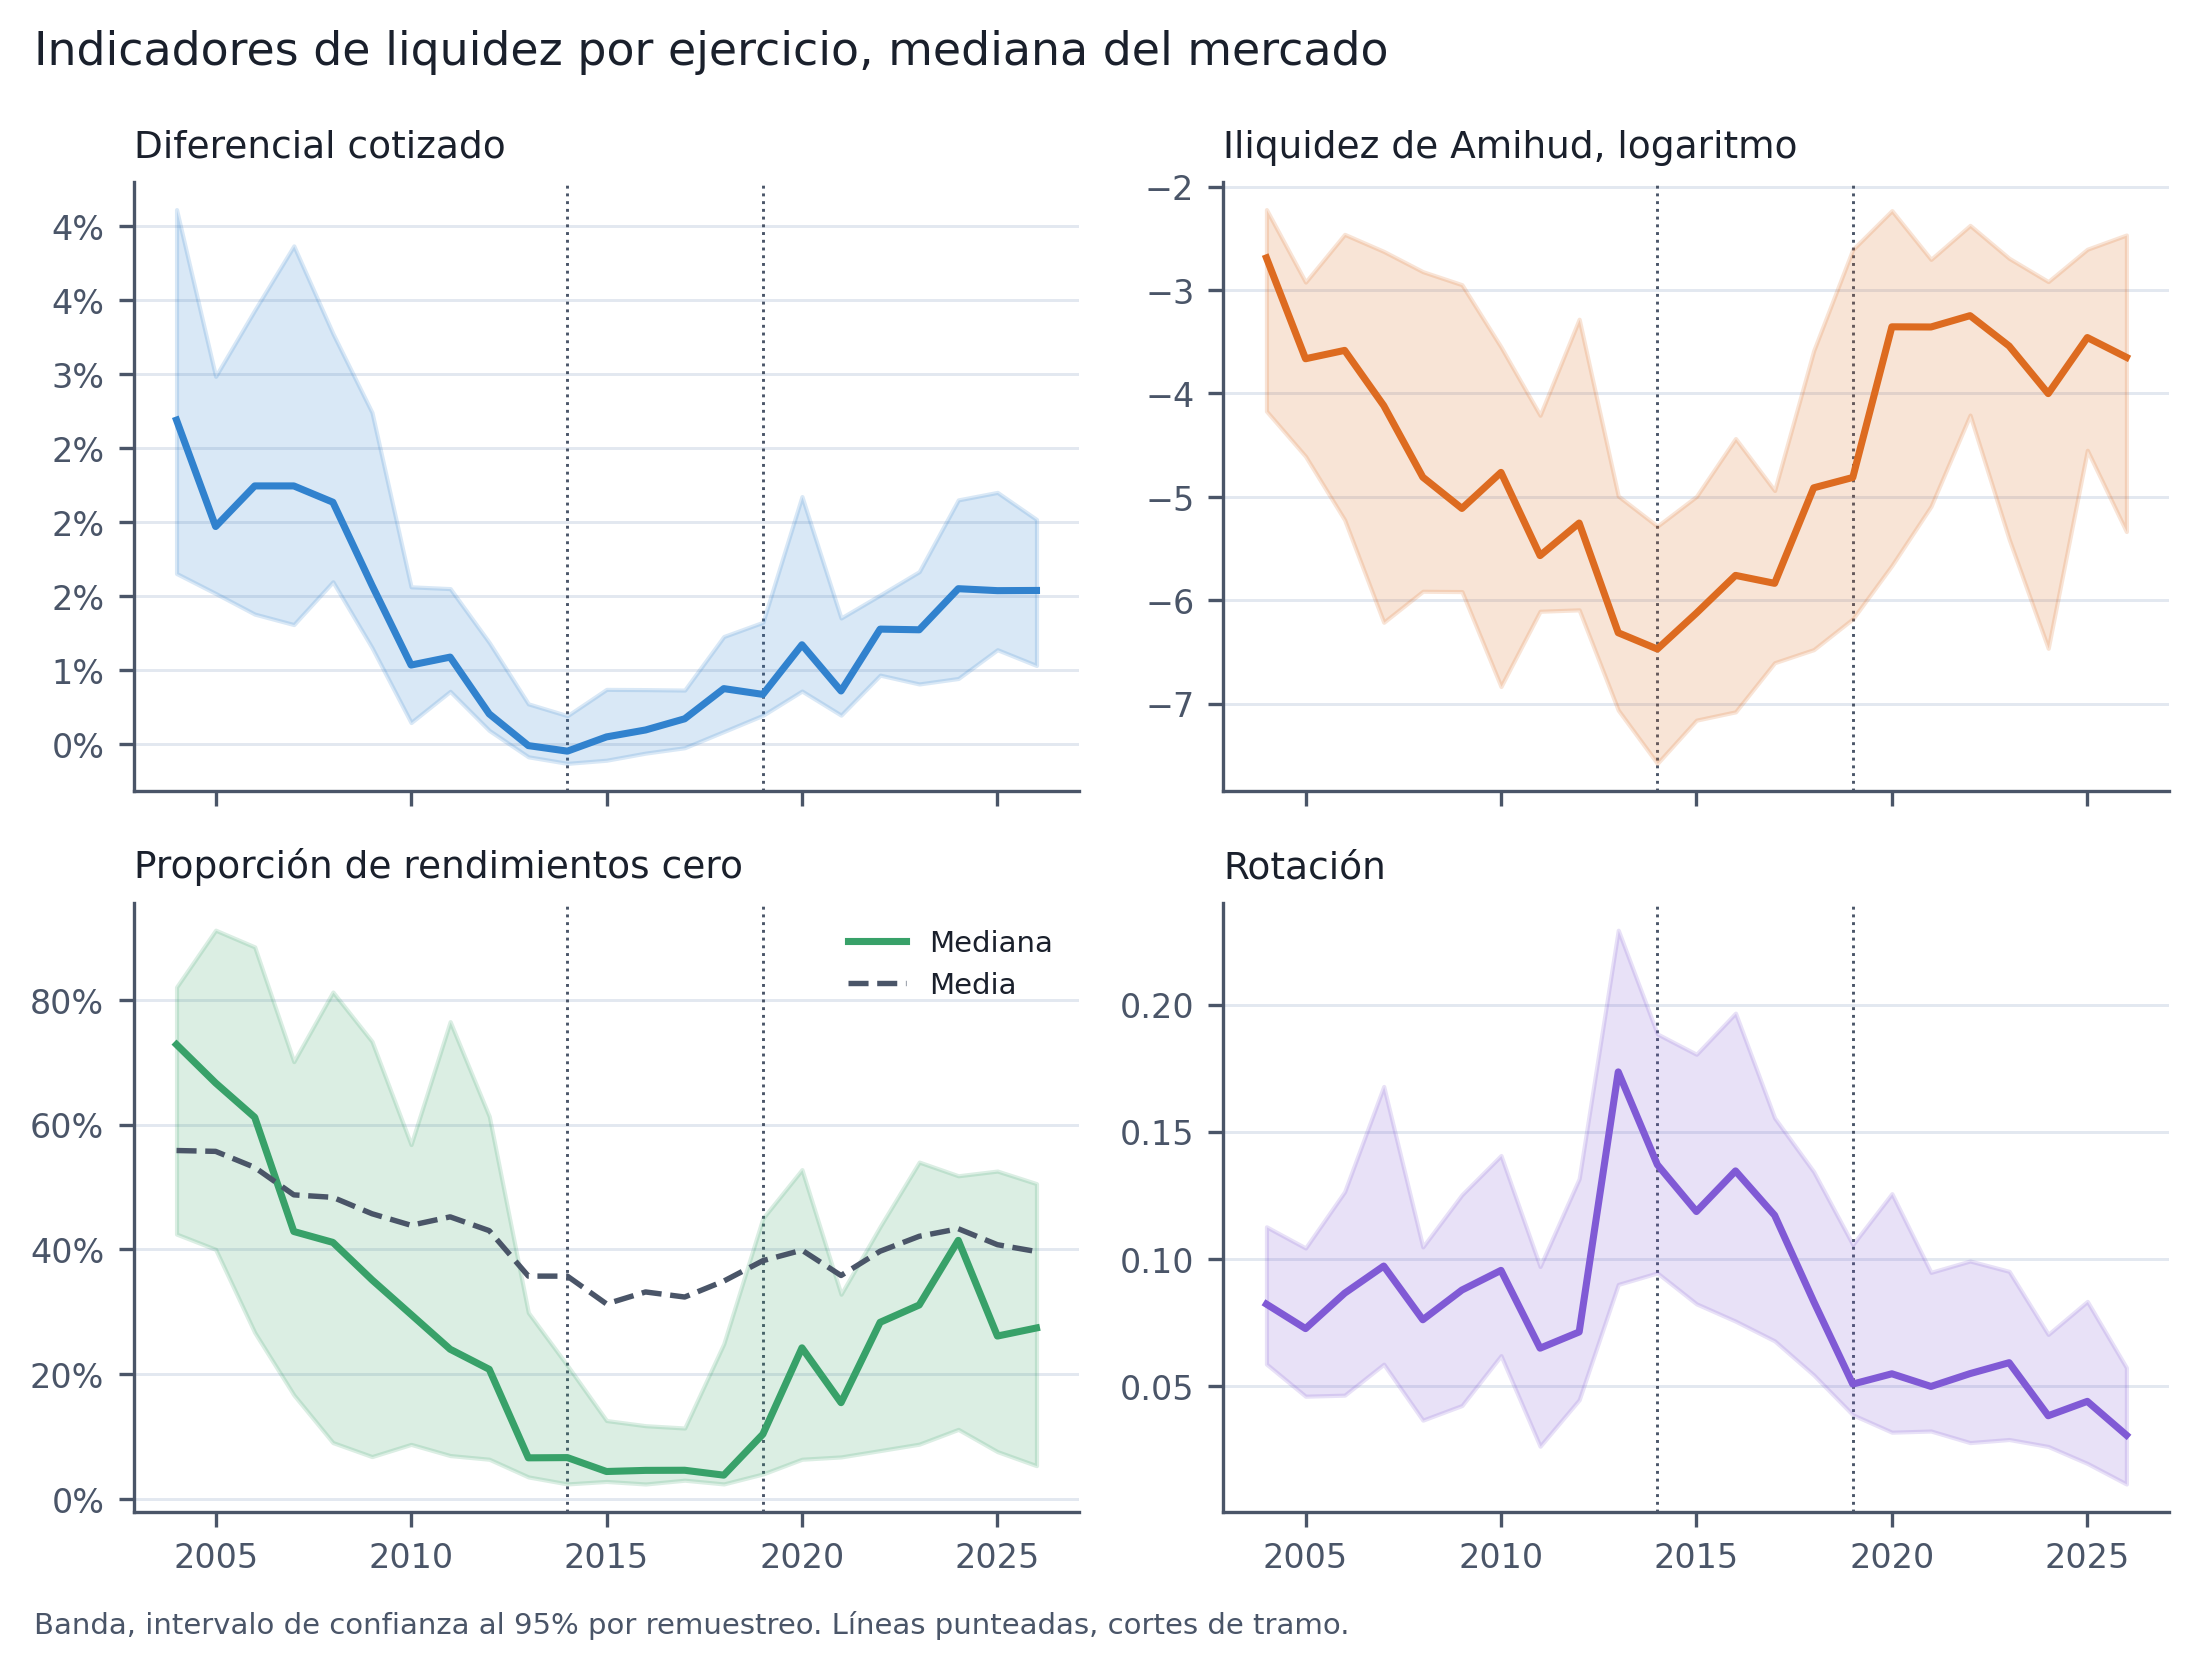
\includegraphics[width=\linewidth]{figuras/figura_4_6.png}\end{center}

\figura{4.6}{Indicadores de liquidez por ejercicio}

\emph{Nota.} Elaboración propia. La banda corresponde al intervalo de confianza al 95\% obtenido por remuestreo. Las líneas punteadas señalan los cortes de tramo. En la proporción de rendimientos cero se reporta también la media, porque su distribución es bimodal, con un grupo de emisoras que opera todas las sesiones y otro que apenas opera, de modo que la mediana cae entre ambas modas.

Los tres paneles de precio dibujan con claridad la forma de U, y el de rotación una loma con cima en 2013. La lectura importante es que la mejora inicial es real y sostenida, lo que contradice la idea de que la liquidez de las emisoras mexicanas se deterioró de manera continua desde el nacimiento del segmento internacional. El deterioro existe y empieza a mediados de la década pasada, en un tramo en que el segmento internacional todavía crecía 21.81\% real anual, de modo que las dos trayectorias no se ordenan de manera simple.

Las bandas también dicen algo. Un intervalo de confianza representa la incertidumbre que rodea una estimación, y aquí se obtiene por remuestreo, es decir, recalculando la mediana miles de veces sobre muestras extraídas de las propias empresas. Una banda ancha indica que la mediana de ese ejercicio está estimada con poca precisión, lo que ocurre sobre todo en los años con menos emisoras y en la iliquidez de Amihud, cuyo indicador es más disperso entre emisoras. Las bandas de los años recientes no se traslapan con las de los años centrales del periodo, lo que es coherente con el deterioro, aunque la evidencia formal del cambio son las pruebas de los apartados 4.4.2 y 4.4.3 y no la comparación visual de los intervalos.

\subseccion{4.4.2 Comparación entre tramos}

La prueba de Wilcoxon compara a cada empresa consigo misma entre dos tramos, de modo que mide el cambio de las mismas emisoras y no la diferencia entre grupos distintos. Es la prueba adecuada cuando interesa saber si las empresas cambiaron, porque una comparación entre grupos distintos podría reflejar simplemente que entraron o salieron emisoras diferentes. Como se aplica a cuatro indicadores por comparación, las probabilidades se ajustan con el procedimiento de Holm.

\tabla{4.9}{Comparación pareada entre tramos, prueba de Wilcoxon}

{\small
\begin{longtable}[]{@{}
  >{\raggedright\arraybackslash}p{(\linewidth - 8\tabcolsep) * \real{0.2001}}
  >{\raggedright\arraybackslash}p{(\linewidth - 8\tabcolsep) * \real{0.2001}}
  >{\raggedright\arraybackslash}p{(\linewidth - 8\tabcolsep) * \real{0.2000}}
  >{\raggedright\arraybackslash}p{(\linewidth - 8\tabcolsep) * \real{0.1999}}
  >{\raggedright\arraybackslash}p{(\linewidth - 8\tabcolsep) * \real{0.1999}}@{}}
\toprule\noalign{}
\begin{minipage}[b]{\linewidth}\raggedright
\textbf{Comparación}
\end{minipage} & \begin{minipage}[b]{\linewidth}\raggedright
\textbf{Indicador}
\end{minipage} & \begin{minipage}[b]{\linewidth}\raggedright
\textbf{Empresas}
\end{minipage} & \begin{minipage}[b]{\linewidth}\raggedright
\textbf{Mediana del cambio}
\end{minipage} & \begin{minipage}[b]{\linewidth}\raggedright
\textbf{p ajustada}
\end{minipage} \\
\midrule\noalign{}
\endhead
\bottomrule\noalign{}
\endlastfoot
2004-2013 a 2014-2018 & Diferencial & 108 & $-$0.42 pp & \textless{} 0.001 \\
& Iliquidez & 107 & $-$0.478 & 0.041 \\
& Rendimientos cero & 119 & 0.00 pp & 0.620 \\
& Rotación & 120 & $-$0.46 pp & 0.252 \\
2014-2018 a 2019-2025 & Diferencial & 116 & +0.22 pp & 0.079 \\
& Iliquidez & 115 & +0.322 & 0.001 \\
& Rendimientos cero & 126 & 0.00 pp & 0.241 \\
& Rotación & 126 & $-$0.48 pp & 0.025 \\
2004-2013 a 2019-2025 & Diferencial & 99 & $-$0.26 pp & 0.001 \\
& Iliquidez & 98 & $-$0.151 & 0.950 \\
& Rendimientos cero & 107 & $-$0.24 pp & 0.950 \\
& Rotación & 108 & $-$0.62 pp & 0.202 \\
\end{longtable}
}

\emph{Nota.} Elaboración propia. Probabilidades ajustadas por Holm dentro de cada comparación. Solo participan las empresas presentes en ambos tramos.

La comparación de punta a punta, del primer al tercer tramo, muestra que el diferencial cotizado mejoró de forma significativa, y que ningún otro indicador cambió de manera significativa. La comparación entre el segundo y el tercer tramo muestra lo contrario, con deterioro en tres de los cuatro indicadores (la mediana del cambio de los rendimientos cero es nula), significativo en la iliquidez de Amihud y en la rotación.

Entre 2014-2018 y 2019-2025 la iliquidez de Amihud de la empresa mediana aumentó 0.322 unidades logarítmicas, la rotación disminuyó 0.48 puntos porcentuales y el diferencial cotizado aumentó 0.22 puntos porcentuales. Las tres cifras describen lo mismo, que es un mayor costo de ejecutar una operación y una menor actividad relativa de las emisoras mexicanas en el periodo reciente. Las dos primeras tienen probabilidad ajustada menor a 5\% y la del diferencial es 0.079. La iliquidez de Amihud se expresa en logaritmo porque su distribución es muy asimétrica, de modo que un aumento de 0.322 unidades logarítmicas equivale a un aumento de alrededor de 38\% en el indicador original, es decir, en el impacto que un peso operado tiene sobre el precio.

Las dos comparaciones no se contradicen. Describen tramos distintos de la misma trayectoria en forma de U, y el hecho de que la comparación de punta a punta arroje mejora mientras la del tramo reciente arroje deterioro es exactamente lo que una trayectoria en U produce.

La regresión de panel sobre indicadoras de tramo, estimada sin efectos fijos por empresa y con errores agrupados por empresa, incorpora también a las empresas presentes en un solo tramo. Sus resultados apuntan en la misma dirección que el contraste pareado, de modo que la conclusión no depende de haber restringido la comparación a las empresas que sobrevivieron al periodo. Esa coincidencia importa porque el contraste pareado solo puede usar empresas presentes en ambos tramos, que tienden a ser las más líquidas.

\subseccion{4.4.3 Diferencias por tamaño}

\tabla{4.10}{Comparación del cambio entre tramos por tercil de capitalización}

{\small
\begin{longtable}[]{@{}
  >{\raggedright\arraybackslash}p{(\linewidth - 8\tabcolsep) * \real{0.2002}}
  >{\raggedright\arraybackslash}p{(\linewidth - 8\tabcolsep) * \real{0.2001}}
  >{\raggedright\arraybackslash}p{(\linewidth - 8\tabcolsep) * \real{0.1999}}
  >{\raggedright\arraybackslash}p{(\linewidth - 8\tabcolsep) * \real{0.1999}}
  >{\raggedright\arraybackslash}p{(\linewidth - 8\tabcolsep) * \real{0.1999}}@{}}
\toprule\noalign{}
\begin{minipage}[b]{\linewidth}\raggedright
\textbf{Comparación}
\end{minipage} & \begin{minipage}[b]{\linewidth}\raggedright
\textbf{Indicador}
\end{minipage} & \begin{minipage}[b]{\linewidth}\raggedright
\textbf{Mediana del primer grupo}
\end{minipage} & \begin{minipage}[b]{\linewidth}\raggedright
\textbf{Mediana del grupo de mayor tamaño}
\end{minipage} & \begin{minipage}[b]{\linewidth}\raggedright
\textbf{p ajustada}
\end{minipage} \\
\midrule\noalign{}
\endhead
\bottomrule\noalign{}
\endlastfoot
Menor frente a mayor & Diferencial & $-$0.45 pp & $-$0.20 pp & 1.000 \\
& Iliquidez & +0.110 & $-$0.850 & 0.425 \\
& Rendimientos cero & 0.00 pp & $-$0.59 pp & 1.000 \\
& \textbf{Rotación} & \textbf{$-$1.87 pp} & \textbf{+2.48 pp} & \textbf{0.025} \\
Intermedia frente a mayor & Diferencial & $-$0.76 pp & $-$0.20 pp & 1.000 \\
& Iliquidez & +0.567 & $-$0.850 & 0.161 \\
& Rendimientos cero & $-$0.08 pp & $-$0.59 pp & 1.000 \\
& Rotación & $-$0.62 pp & +2.48 pp & 0.596 \\
\end{longtable}
}

\emph{Nota.} Elaboración propia. Cambio entre 2004-2013 y 2019-2025. Prueba de Mann y Whitney con corrección de Holm sobre las doce comparaciones de la familia, que son los tres pares de terciles por los cuatro indicadores. La tabla muestra las ocho que contrastan contra el tercil de mayor tamaño.

De las ocho comparaciones, una sola resulta significativa, que es la de rotación entre el tercil de menor tamaño y el de mayor. Las empresas pequeñas perdieron 1.87 puntos porcentuales de rotación mientras las grandes ganaron 2.48, y esa diferencia es poco compatible con la hipótesis de que ambos grupos cambiaron igual. Ninguna comparación del tercil intermedio contra el de mayor tamaño resulta significativa.

La prueba de Mann y Whitney compara dos grupos independientes y pregunta si los valores de uno tienden a ser mayores que los del otro. Aquí los valores comparados son cambios, no niveles, de modo que la prueba responde si las emisoras pequeñas empeoraron más que las grandes y no si están peor que ellas. Esa distinción es central para esta hipótesis y conviene subrayarla, porque las emisoras pequeñas están peor en los cuatro indicadores durante todo el periodo, y eso no es lo que la hipótesis afirma.

\begin{center}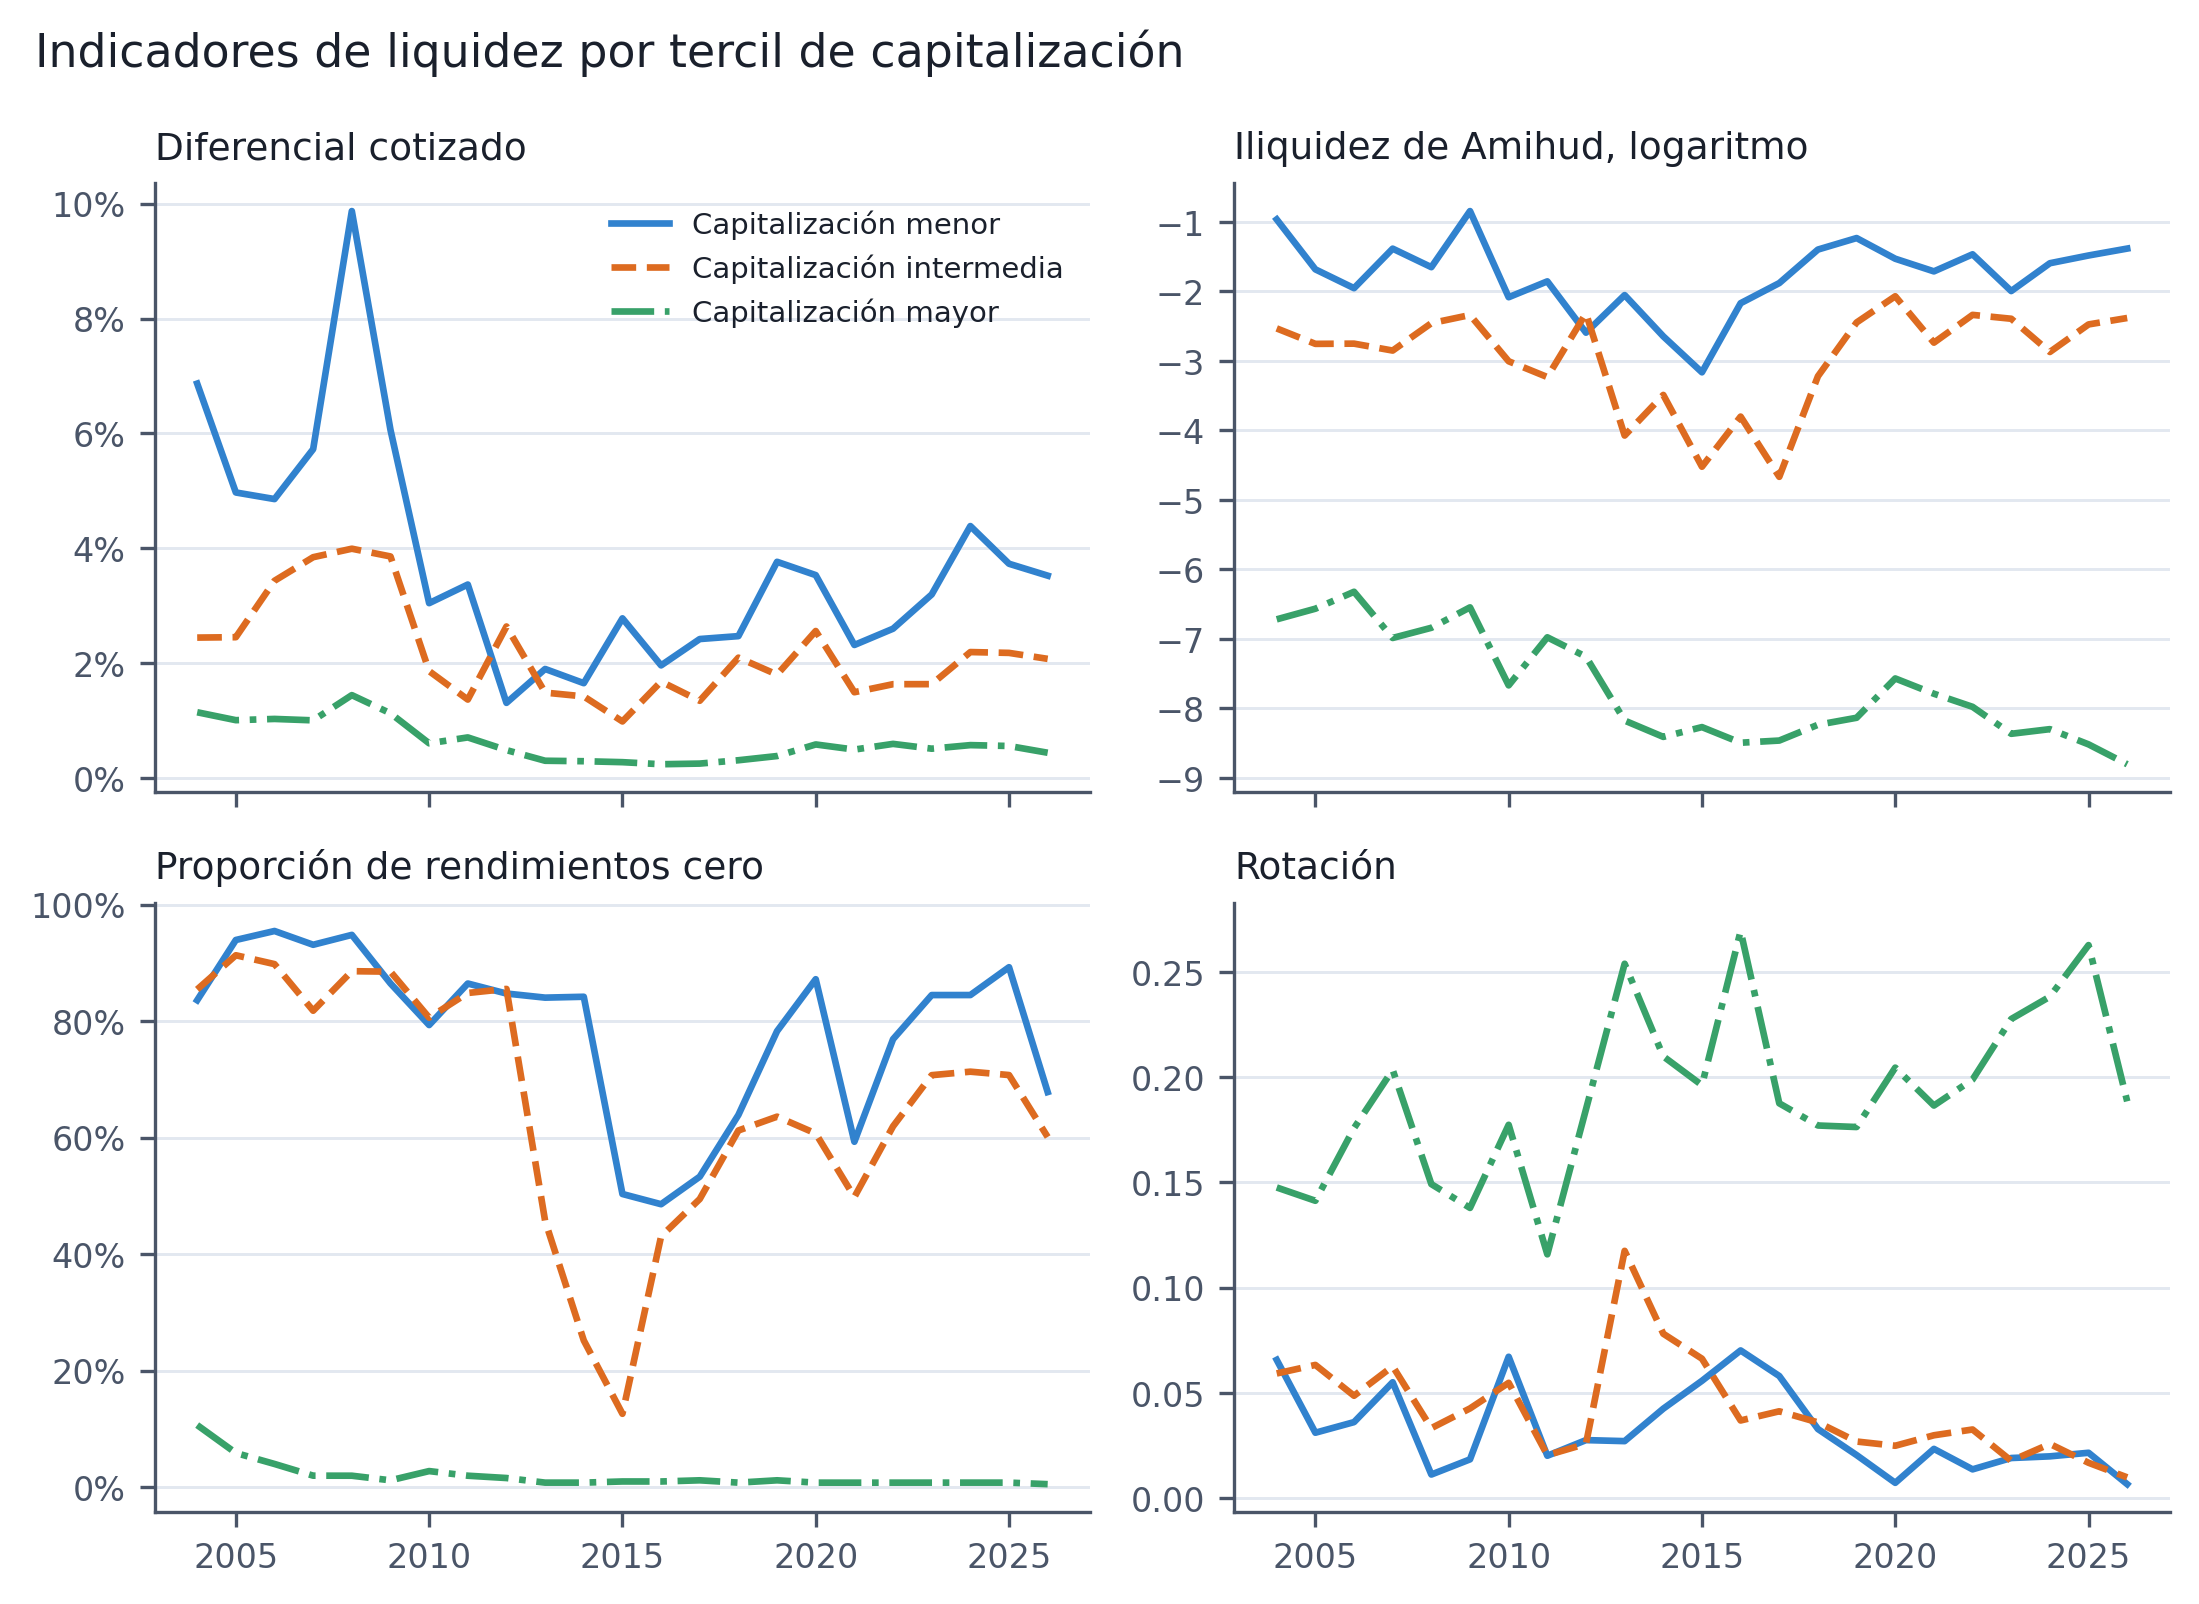
\includegraphics[width=\linewidth]{figuras/figura_4_7.png}\end{center}

\figura{4.7}{Indicadores de liquidez por tercil de capitalización}

\emph{Nota.} Elaboración propia. Mediana anual dentro de cada tercil.

Las líneas de los tres terciles casi no se cruzan en ninguno de los cuatro paneles, lo que indica que las diferencias de nivel entre emisoras grandes y pequeñas son persistentes durante los veintidós años. Las emisoras del tercil menor tienen diferenciales más altos, mayor iliquidez, más sesiones sin movimiento de precio y menor rotación en prácticamente todos los ejercicios. Esa jerarquía es estable y no constituye evidencia a favor de la hipótesis, que afirma algo distinto, que es que el deterioro del periodo las afectó más. La figura muestra niveles, la tabla 4.10 contrasta cambios, y las dos cosas no deben confundirse.

\begin{center}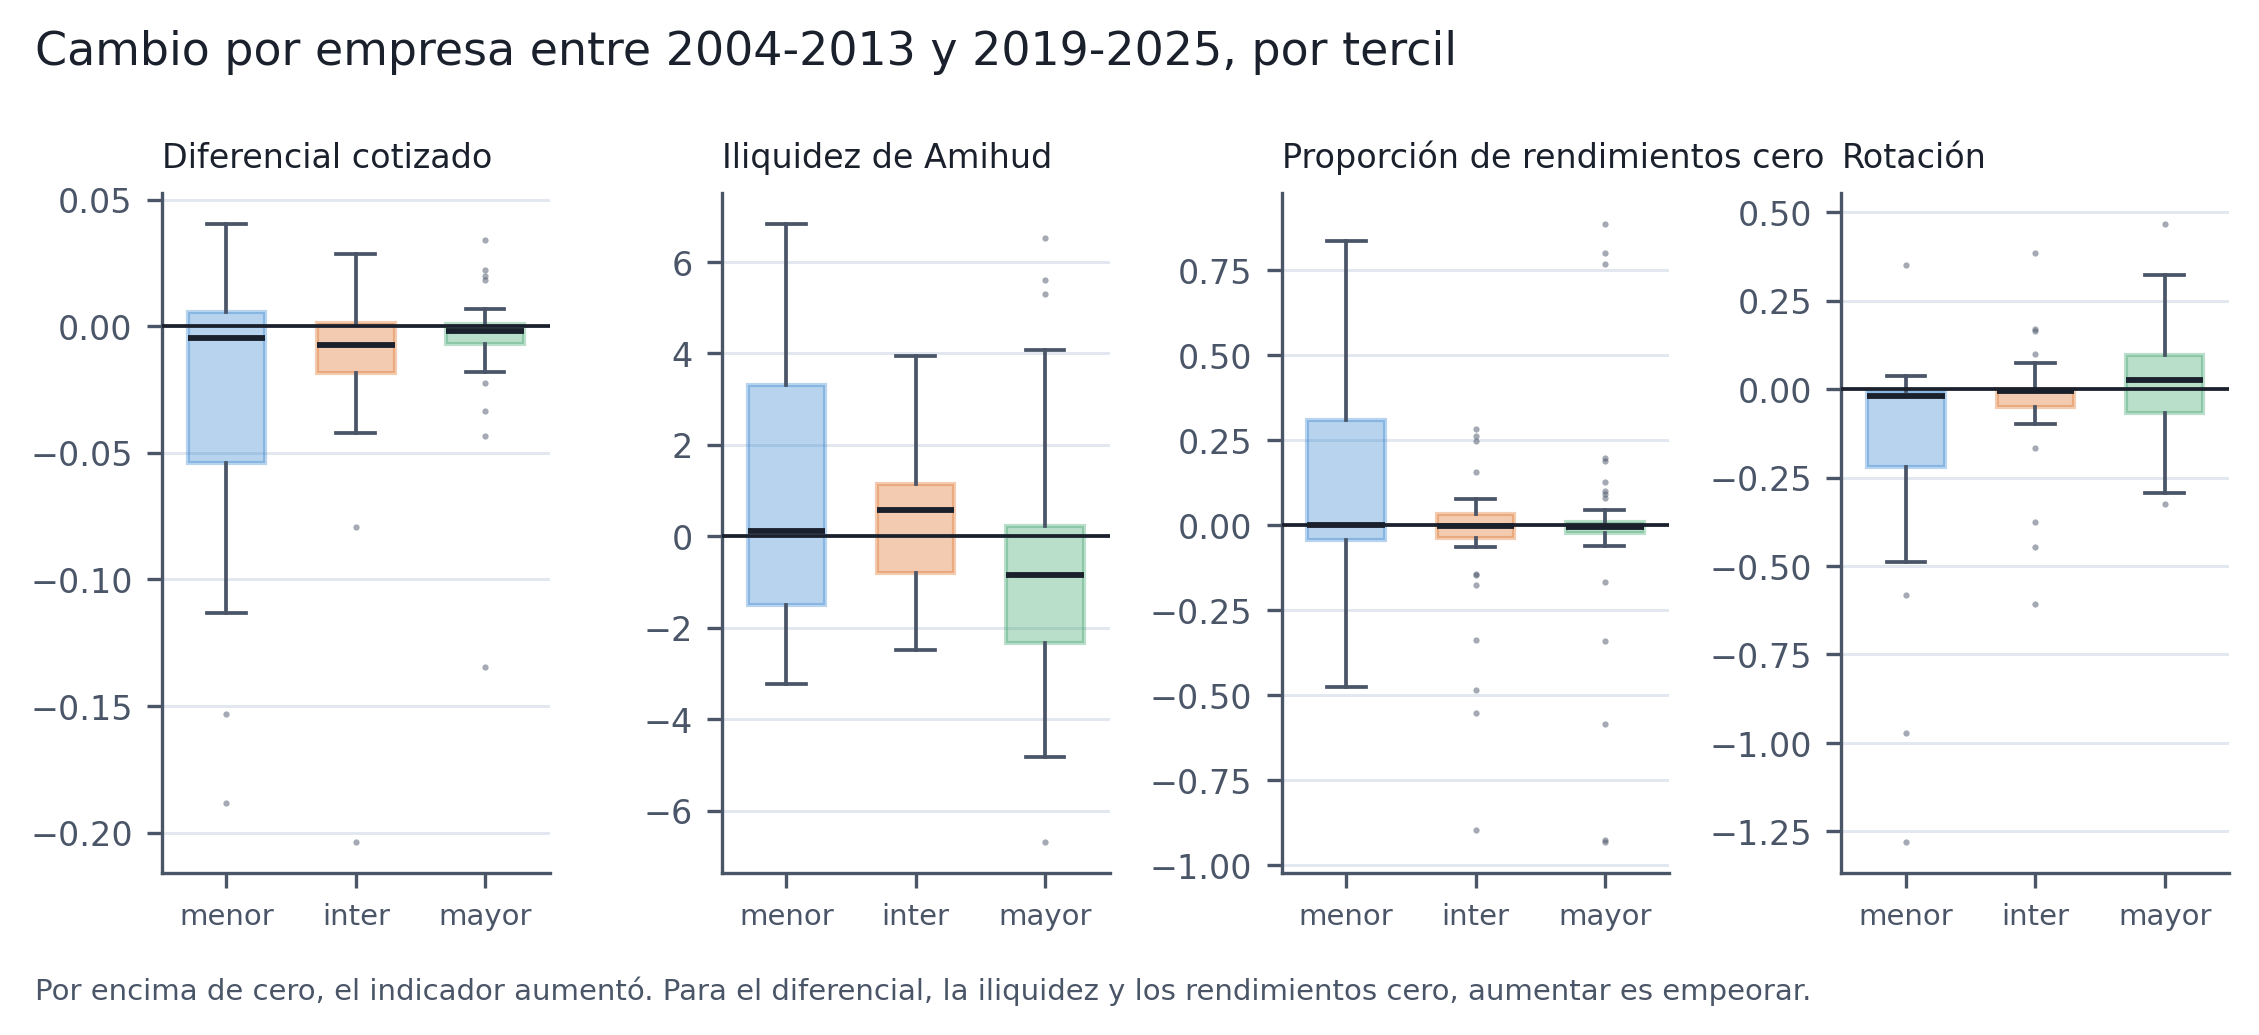
\includegraphics[width=\linewidth]{figuras/figura_4_8.png}\end{center}

\figura{4.8}{Cambio por empresa entre 2004-2013 y 2019-2025, por tercil}

\emph{Nota.} Elaboración propia. Por encima de cero el indicador aumentó. En el diferencial, la iliquidez y los rendimientos cero, aumentar significa empeorar.

Esta figura sí contrasta cambios, y lo que salta a la vista no es un desplazamiento de las cajas del tercil menor hacia el deterioro, sino su amplitud. Las cajas del tercil menor son considerablemente más amplias que las del mayor en los cuatro indicadores, es decir, a las emisoras pequeñas les ocurrió de todo, mientras que a las grandes les ocurrió poco y parecido. Esa diferencia de dispersión se describe pero no se contrasta estadísticamente, porque las pruebas de este apartado comparan posiciones centrales y no dispersiones.

La heterogeneidad de las emisoras pequeñas tiene una consecuencia práctica. Hablar de la emisora pequeña mexicana como un grupo homogéneo es inexacto, porque dentro de ese tercil conviven empresas que mejoraron mucho y empresas que se deterioraron mucho. Una política dirigida a ese segmento tendría que distinguir entre unas y otras.

El apartado 3.4.2 anuncia además un examen que no depende del corte en terciles, que consiste en relacionar el cambio de liquidez con el logaritmo de la capitalización tratada como variable continua. Esa relación resulta significativa en la iliquidez de Amihud, con pendiente de $-$0.338 y probabilidad de 0.015, y en la rotación, con pendiente de +0.037 y probabilidad de 0.016. En ambos casos el signo indica que las empresas más grandes cambiaron en mejor dirección que las pequeñas, lo que apunta en el sentido de la hipótesis, aunque el coeficiente de determinación es de 0.053 y 0.078, de modo que el tamaño explica una parte pequeña de la variación de los cambios.

\subseccion{4.4.4 Lectura de la hipótesis}

\textbf{H2a.} Entre 2014--2018 y 2019--2025 la iliquidez de Amihud aumentó 0.322 unidades logarítmicas ($p$ ajustada 0.001) y la rotación disminuyó 0.48 puntos porcentuales ($p$ ajustada 0.025), mientras que el diferencial aumentó 0.22 puntos con $p$ ajustada de 0.079 (Tabla 4.9). Dentro del tramo 2019--2025 las pruebas de tendencia detectan deterioro en los cuatro indicadores (Tabla 4.8). H2a se sostiene.

\textbf{H2b.} La comparación por tamaño debe hacerse en la ventana del deterioro. La Tabla 4.10 compara 2004--2013 con 2019--2025, un periodo de mejora neta del diferencial; la Tabla 4.20 repite el contraste entre 2014--2018 y 2019--2025.

\tabla{4.20}{Cambio entre 2014--2018 y 2019--2025 por tercil de capitalización}
\begin{center}\small
\begin{tabular}{@{}llcrrr@{}}\toprule
Indicador & Grupo & $n$ (grupo / mayor) & Cambio grupo & Cambio mayor & $p$ Holm\\\midrule
\tablainput{tabla_tamano}
\bottomrule\end{tabular}
\end{center}
\emph{Nota.} Elaboración propia. Mediana del cambio por emisora; puntos porcentuales, salvo $\ln ILLIQ$ en pesos de 2018. Prueba de Mann y Whitney bilateral contra el tercil mayor, corrección de Holm sobre ocho pruebas.

El cambio fue de mayor magnitud en las emisoras de menor capitalización en la iliquidez de Amihud, los rendimientos cero y la rotación, pero con entre 25 y 43 empresas por grupo ninguna diferencia es significativa. H2b no puede confirmarse ni descartarse con estos datos. En el panel mensual, la asociación entre la participación del SIC y los rendimientos cero se concentra en el tercil menor (coeficiente 0.039, $p<0.001$, frente a 0.005 sin significancia en el tercil mayor), el único indicio de heterogeneidad por tamaño de la investigación.

\seccion{4.5 Tercera hipótesis. Relación entre el SIC y la liquidez}

\subseccion{4.5.1 Coeficiente de la participación}

\tabla{4.11}{Coeficiente de la participación del SIC, especificación contemporánea}

{\small
\begin{longtable}[]{@{}
  >{\raggedright\arraybackslash}p{(\linewidth - 14\tabcolsep) * \real{0.1503}}
  >{\raggedright\arraybackslash}p{(\linewidth - 14\tabcolsep) * \real{0.1325}}
  >{\raggedright\arraybackslash}p{(\linewidth - 14\tabcolsep) * \real{0.1504}}
  >{\raggedright\arraybackslash}p{(\linewidth - 14\tabcolsep) * \real{0.0995}}
  >{\raggedright\arraybackslash}p{(\linewidth - 14\tabcolsep) * \real{0.0747}}
  >{\raggedright\arraybackslash}p{(\linewidth - 14\tabcolsep) * \real{0.1072}}
  >{\raggedright\arraybackslash}p{(\linewidth - 14\tabcolsep) * \real{0.1657}}
  >{\raggedright\arraybackslash}p{(\linewidth - 14\tabcolsep) * \real{0.1199}}@{}}
\toprule\noalign{}
\begin{minipage}[b]{\linewidth}\raggedright
\textbf{Indicador}
\end{minipage} & \begin{minipage}[b]{\linewidth}\raggedright
\textbf{Coeficiente}
\end{minipage} & \begin{minipage}[b]{\linewidth}\raggedright
\textbf{Error convencional}
\end{minipage} & \begin{minipage}[b]{\linewidth}\raggedright
\textbf{Error de Driscoll y Kraay}
\end{minipage} & \begin{minipage}[b]{\linewidth}\raggedright
\textbf{p}
\end{minipage} & \begin{minipage}[b]{\linewidth}\raggedright
\textbf{Factor de Moulton}
\end{minipage} & \begin{minipage}[b]{\linewidth}\raggedright
\textbf{Observaciones}
\end{minipage} & \begin{minipage}[b]{\linewidth}\raggedright
\textbf{Empresas}
\end{minipage} \\
\midrule\noalign{}
\endhead
\bottomrule\noalign{}
\endlastfoot
Diferencial cotizado & +0.0004 & 0.0002 & 0.0004 & 0.387 & 2.62 & 22,104 & 184 \\
Iliquidez de Amihud & +0.2235 & 0.0177 & 0.0468 & \textless{} 0.001 & 1.97 & 21,665 & 182 \\
Rendimientos cero & +0.0112 & 0.0017 & 0.0041 & 0.006 & 3.43 & 23,943 & 190 \\
Rotación & $-$0.0015 & 0.0003 & 0.0005 & 0.001 & 1.87 & 23,910 & 190 \\
\end{longtable}
}

\emph{Nota.} Elaboración propia. El coeficiente expresa el cambio asociado a diez puntos porcentuales más de participación. \corregido{decía 0.349; 0.387 como en las Tablas 4.15 a 4.17 (reestimado: 0.385)} Todas las especificaciones incluyen efectos fijos por emisora, tendencia y los controles del apartado 3.3.4, sobre 273 periodos mensuales.

Un error estándar mide la imprecisión de un coeficiente, y su tamaño depende de los supuestos que se hagan sobre cómo se relacionan las observaciones entre sí. Los errores de Driscoll y Kraay (1998) estiman la incertidumbre admitiendo que las emisoras se mueven juntas en un mismo mes y que los periodos están correlacionados entre sí, que son las dos dependencias que un error convencional ignoraría. Son por tanto más grandes y más conservadores, y son los que la investigación usa para decidir significancia.

Tres de los cuatro coeficientes son significativos con esos errores, y los tres tienen el signo que corresponde a un deterioro de las condiciones de negociación. Diez puntos más de participación del SIC se asocian con 0.224 unidades más de iliquidez de Amihud en logaritmo, con 1.12 puntos porcentuales más de rendimientos cero y con 0.15 puntos porcentuales menos de rotación. El coeficiente del diferencial cotizado no resulta distinguible de cero.

Conviene precisar el alcance de estos coeficientes. La palabra asocian es deliberada. El diseño identifica co-movimiento entre dos series y no un efecto causal, de modo que estos coeficientes no autorizan a afirmar que el crecimiento del segmento internacional produjo el deterioro de la liquidez. Las dos series pueden moverse juntas porque un tercer factor mueve a las dos, posibilidad que el apartado 4.5.3 aborda directamente.

Esta estimación en niveles se reporta como contraste y no como la inferencia principal. El apartado 3.4.3 establece que, cuando no puede rechazarse la raíz unitaria, la inferencia se apoya en la estimación en primeras diferencias, y el apartado 4.3.2 mostró que en la serie de participación no se rechaza. Los resultados en primeras diferencias se presentan en el apartado 4.5.5 y conviene leer los de esta tabla a la luz de aquellos.

El factor de Moulton varía entre 1.87 y 3.43. Ese factor indica cuántas veces se subestimaría el error estándar al ignorar que la variable de interés es la misma para todas las emisoras en cada mes, de modo que un valor de 3.43 significa que el error convencional sería alrededor de tres veces y media menor que el apropiado. Se reporta como diagnóstico y no como corrección. Es pertinente recordar que la participación toma el mismo valor para todas las emisoras en cada periodo, de modo que el número de observaciones que informan a su coeficiente es 273, que es el número de periodos, y no las más de veinte mil filas del panel.

\subseccion{4.5.2 Precedencia}

\tabla{4.12}{Quiebres estimados por Bai y Perron sobre las series mensuales}

{\small
\begin{longtable}[]{@{}
  >{\raggedright\arraybackslash}p{(\linewidth - 2\tabcolsep) * \real{0.5000}}
  >{\raggedright\arraybackslash}p{(\linewidth - 2\tabcolsep) * \real{0.5000}}@{}}
\toprule\noalign{}
\begin{minipage}[b]{\linewidth}\raggedright
\textbf{Serie}
\end{minipage} & \begin{minipage}[b]{\linewidth}\raggedright
\textbf{Quiebres estimados}
\end{minipage} \\
\midrule\noalign{}
\endhead
\bottomrule\noalign{}
\endlastfoot
Participación del SIC & dic 2005, dic 2014, feb 2020, abr 2023 \\
Diferencial cotizado & ago 2007, oct 2008, oct 2009, ago 2014 \\
Iliquidez de Amihud & ago 2008, nov 2016, oct 2021, nov 2024 \\
Rendimientos cero & ago 2006, jun 2010, ago 2014, jul 2022 \\
Rotación & ene 2011, oct 2012, jul 2017, dic 2018 \\
\end{longtable}
}

\emph{Nota.} Elaboración propia.

Los quiebres de la participación y los de dos indicadores de liquidez se ubican en la misma zona del periodo. El de la participación ocurre en diciembre de 2014, el de los rendimientos cero en agosto de 2014 y el del diferencial cotizado en octubre de 2014 \revisar{la Tabla 4.12 dice agosto de 2014 para el diferencial}.

Esa coincidencia no establece precedencia en ninguna dirección. Los quiebres de liquidez son cuatro meses anteriores al de la participación, y esa cercanía no permite ordenar las series en el tiempo, porque el procedimiento estima la fecha del quiebre con incertidumbre y el mínimo de doce meses por segmento restringe dónde puede colocarlo. Lo que sí permite afirmar es que los quiebres de la liquidez no ocurren mucho antes que el de la participación. Si así hubiera sido, se debilitaría la lectura de que la participación antecede al cambio de liquidez, aunque no se descartaría una asociación en sentido inverso. La especificación con participación rezagada uno y tres periodos complementa este examen, y sus coeficientes mantienen signo y significancia, de modo que la asociación no depende de leer las dos series en el mismo mes.

\begin{center}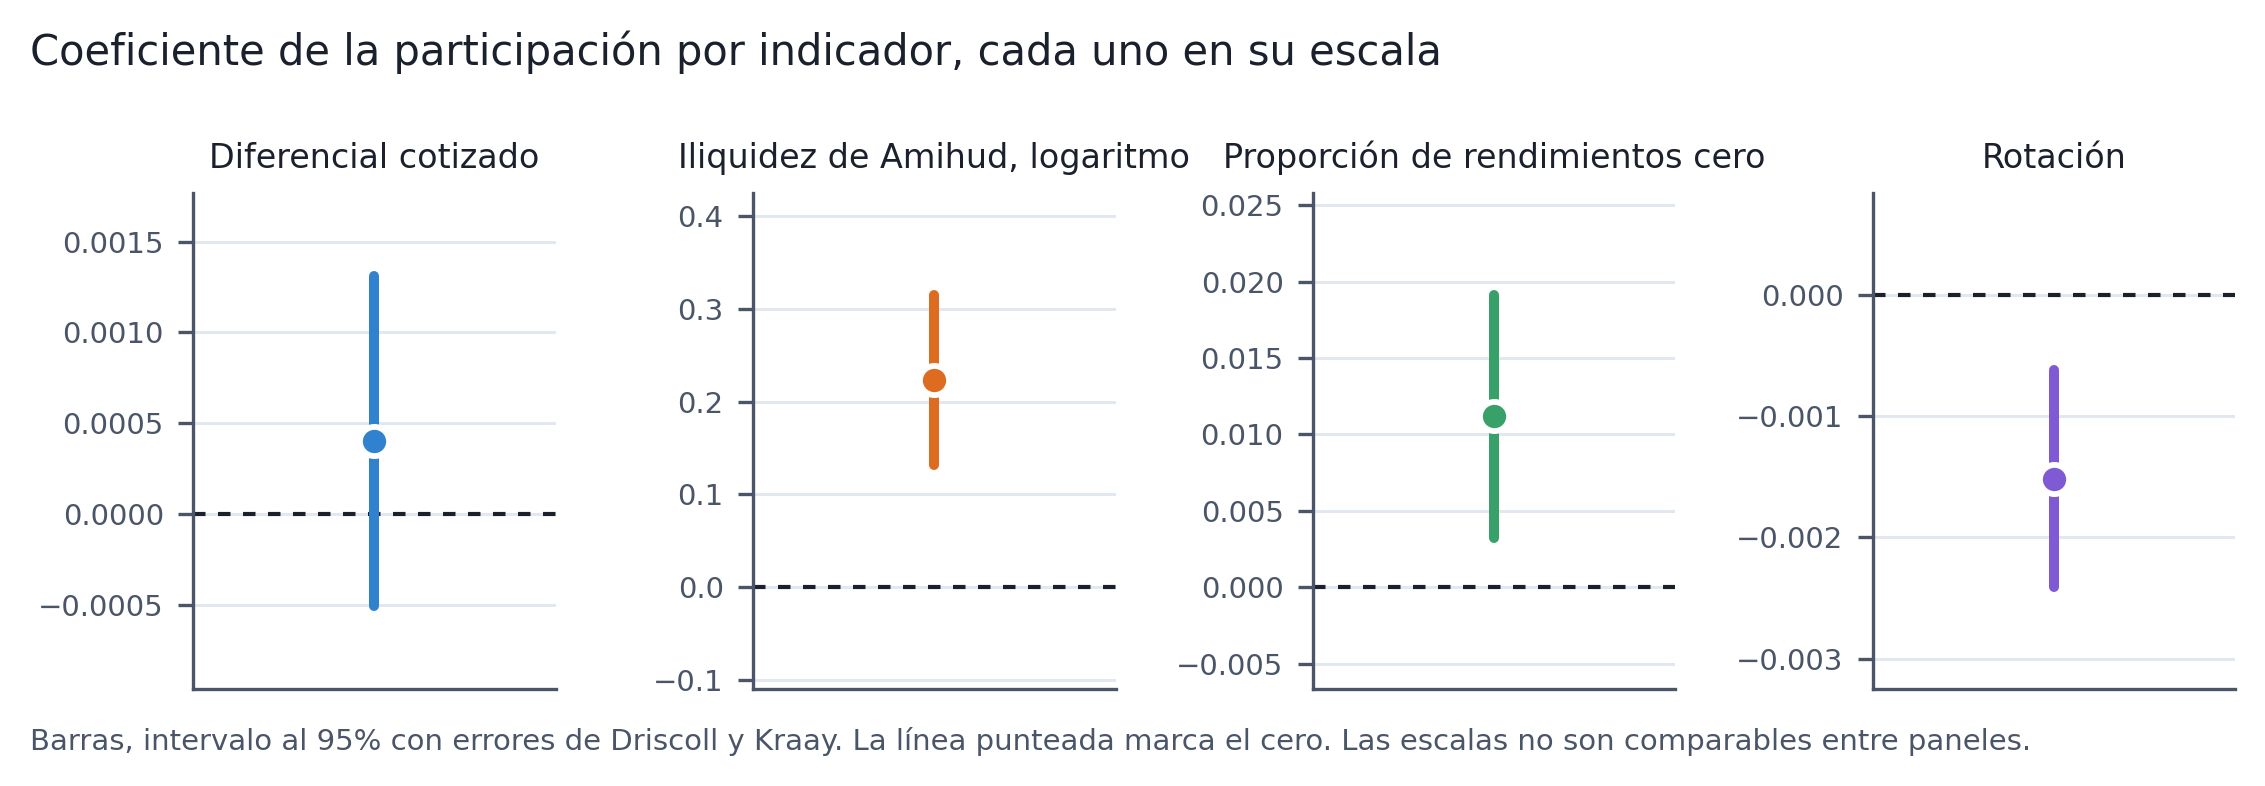
\includegraphics[width=\linewidth]{figuras/figura_4_9.png}\end{center}

\figura{4.9}{Coeficiente de la participación del SIC por indicador}

\emph{Nota.} Elaboración propia. Las barras representan el intervalo al 95\% con errores estándar de Driscoll y Kraay (1998), y la línea punteada marca el cero.

Cada indicador va en su propio panel y con su propia escala, porque las cuatro variables dependientes tienen unidades distintas, de modo que la longitud de las barras no debe compararse visualmente entre paneles. Dentro de cada panel, lo que importa es si la barra cruza la línea del cero. Un intervalo que cruza el cero indica que el coeficiente no se distingue estadísticamente de cero, lo que ocurre únicamente en el diferencial cotizado. En los otros tres paneles la barra queda completamente a un lado de la línea, lo que corresponde a los tres coeficientes significativos de la tabla 4.11.

\subseccion{4.5.3 Poder explicativo incremental}

\tabla{4.13}{Variación adicional que aporta cada bloque}

{\small
\begin{longtable}[]{@{}
  >{\raggedright\arraybackslash}p{(\linewidth - 8\tabcolsep) * \real{0.1972}}
  >{\raggedright\arraybackslash}p{(\linewidth - 8\tabcolsep) * \real{0.2185}}
  >{\raggedright\arraybackslash}p{(\linewidth - 8\tabcolsep) * \real{0.1975}}
  >{\raggedright\arraybackslash}p{(\linewidth - 8\tabcolsep) * \real{0.1947}}
  >{\raggedright\arraybackslash}p{(\linewidth - 8\tabcolsep) * \real{0.1921}}@{}}
\toprule\noalign{}
\begin{minipage}[b]{\linewidth}\raggedright
\textbf{Indicador}
\end{minipage} & \begin{minipage}[b]{\linewidth}\raggedright
\textbf{Controles financieros y macroeconómicos}
\end{minipage} & \begin{minipage}[b]{\linewidth}\raggedright
\textbf{Participación del SIC}
\end{minipage} & \begin{minipage}[b]{\linewidth}\raggedright
\textbf{Diferencia por orden de entrada}
\end{minipage} & \begin{minipage}[b]{\linewidth}\raggedright
\textbf{Razón entre bloques}
\end{minipage} \\
\midrule\noalign{}
\endhead
\bottomrule\noalign{}
\endlastfoot
Diferencial cotizado & 3.84\% & 0.01\% & +0.18\% & 480 a 1 \\
Iliquidez de Amihud & 9.75\% & 0.66\% & +1.57\% & 15 a 1 \\
Rendimientos cero & 8.01\% & 0.16\% & $-$0.12\% & 49 a 1 \\
Rotación & 4.46\% & 0.11\% & +0.18\% & 42 a 1 \\
\end{longtable}
}

\emph{Nota.} Elaboración propia. Incremento del coeficiente de determinación intragrupo al añadir cada bloque, sobre la misma muestra. \corregido{razón verificada al reestimar: 481. Con el orden de entrada inverso es 20 para el diferencial y 3.7 para Amihud} El bloque de controles contiene seis variables y el de la participación una. La última columna de porcentajes es la diferencia entre el incremento de un bloque según entre primero o segundo, de modo que no es una intersección de varianzas y puede resultar negativa, como ocurre en los rendimientos cero, cuando un bloque mejora el ajuste del otro al entrar junto con él.

Indica cuánto mejora el ajuste de un modelo cuando se incorpora un conjunto de variables que antes no estaba incluido. El coeficiente de determinación intragrupo es la proporción de la variación que el modelo explica una vez descontadas las diferencias permanentes entre empresas, es decir, mide qué tan bien se explican los cambios de cada empresa a lo largo del tiempo y no las diferencias entre una empresa y otra.

En los cuatro indicadores el bloque de controles aporta más variación adicional que la participación del SIC, con razones que van de quince a uno hasta cuatrocientos ochenta a uno. En la iliquidez de Amihud, por ejemplo, los controles agregan 9.75 puntos porcentuales al coeficiente de determinación intragrupo, frente a 0.66 puntos de la participación. La diferencia es menor en ese indicador, que es también el único donde el coeficiente de la participación sobrevive en primeras diferencias.

Esa comparación tiene un alcance definido. Que el bloque de controles aporte más ajuste no implica que cada control individual sea más importante que la participación, ni que los controles causen los cambios de liquidez. La comparación es entre conjuntos de variables y entre magnitudes de ajuste, dentro de la especificación estimada en niveles.

Esa comparación requiere dos precisiones que el capítulo III estableció de antemano. La primera es que enfrenta un bloque de seis variables contra una sola, y un conjunto mayor de regresores explica mecánicamente más variación. La segunda es que un incremento mayor que otro no constituye por sí mismo una diferencia estadísticamente demostrada. El intervalo construido por remuestreo por empresa y por bloques de doce meses consecutivos no incluye el cero en ninguno de los cuatro indicadores, de modo que la diferencia entre ambos incrementos está estimada con precisión suficiente para sostener la comparación.

\begin{center}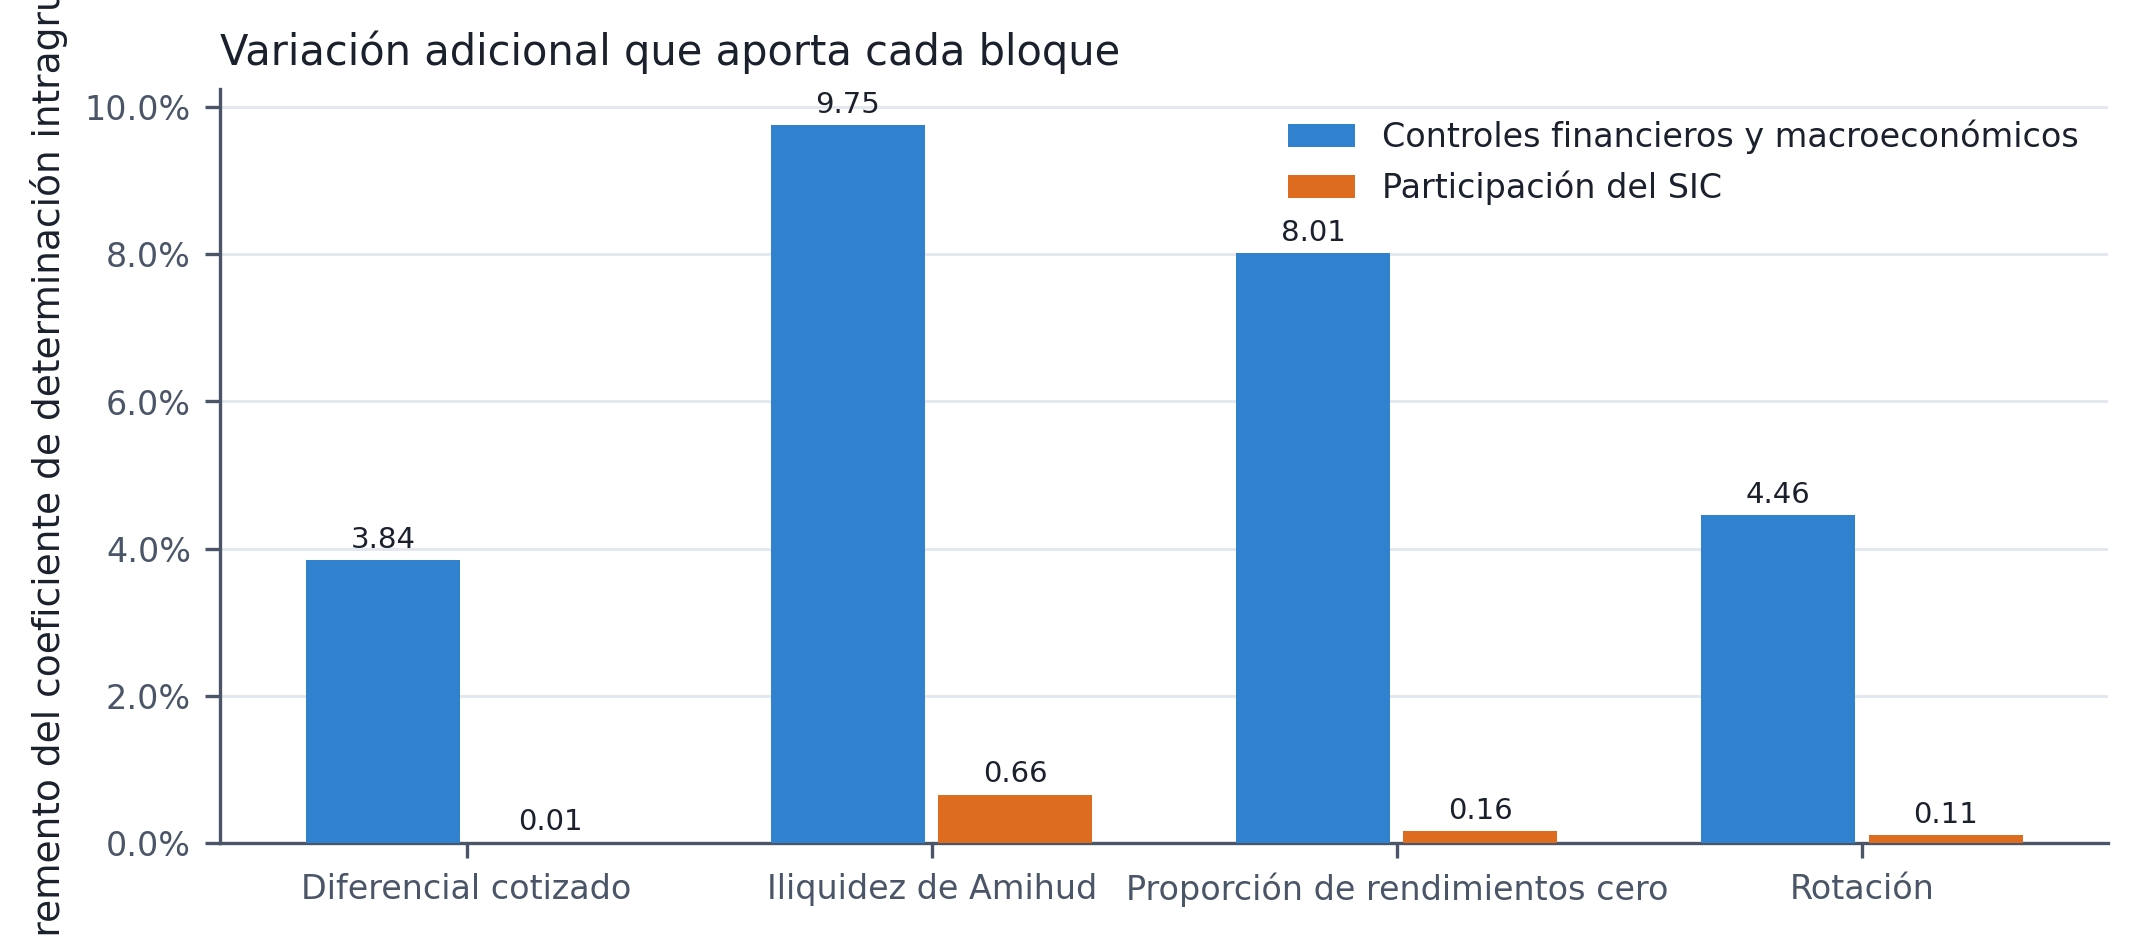
\includegraphics[width=\linewidth]{figuras/figura_4_10.png}\end{center}

\figura{4.10}{Variación adicional que aporta cada bloque}

\emph{Nota.} Elaboración propia. Incremento del coeficiente de determinación intragrupo al incorporar cada bloque.

La desproporción entre las dos barras de cada indicador es el resultado central de esta hipótesis y la figura la vuelve inmediata. La barra de la participación apenas se distingue del eje en tres de los cuatro indicadores. El único caso donde alcanza una altura visible es la iliquidez de Amihud, que es coherente con que sea también el indicador de coeficiente más fuerte y el único que resiste la estimación en primeras diferencias.

El apartado 3.3.4 anuncia además un diagnóstico de los controles, porque varios se mueven juntos y conviene saber cuánto de cada coeficiente depende de la presencia de los demás.

\tabla{4.14}{Correlación entre los controles}

{\small
\begin{longtable}[]{@{}
  >{\raggedright\arraybackslash}p{(\linewidth - 12\tabcolsep) * \real{0.1614}}
  >{\raggedright\arraybackslash}p{(\linewidth - 12\tabcolsep) * \real{0.1643}}
  >{\raggedright\arraybackslash}p{(\linewidth - 12\tabcolsep) * \real{0.1458}}
  >{\raggedright\arraybackslash}p{(\linewidth - 12\tabcolsep) * \real{0.1267}}
  >{\raggedright\arraybackslash}p{(\linewidth - 12\tabcolsep) * \real{0.1293}}
  >{\raggedright\arraybackslash}p{(\linewidth - 12\tabcolsep) * \real{0.1267}}
  >{\raggedright\arraybackslash}p{(\linewidth - 12\tabcolsep) * \real{0.1458}}@{}}
\toprule\noalign{}
\begin{minipage}[b]{\linewidth}\raggedright
\end{minipage} & \begin{minipage}[b]{\linewidth}\raggedright
\textbf{Rendimiento}
\end{minipage} & \begin{minipage}[b]{\linewidth}\raggedright
\textbf{Volatilidad sistemática}
\end{minipage} & \begin{minipage}[b]{\linewidth}\raggedright
\textbf{Tasa}
\end{minipage} & \begin{minipage}[b]{\linewidth}\raggedright
\textbf{Tipo de cambio}
\end{minipage} & \begin{minipage}[b]{\linewidth}\raggedright
\textbf{VIX}
\end{minipage} & \begin{minipage}[b]{\linewidth}\raggedright
\textbf{Volatilidad propia}
\end{minipage} \\
\midrule\noalign{}
\endhead
\bottomrule\noalign{}
\endlastfoot
Rendimiento de mercado & 1.000 & $-$0.177 & $-$0.051 & $-$0.094 & $-$0.118 & $-$0.024 \\
Volatilidad sistemática & $-$0.177 & 1.000 & 0.082 & $-$0.076 & 0.712 & 0.214 \\
Tasa de interés & $-$0.051 & 0.082 & 1.000 & 0.164 & $-$0.054 & $-$0.032 \\
Tipo de cambio & $-$0.094 & $-$0.076 & 0.164 & 1.000 & 0.144 & $-$0.073 \\
VIX & $-$0.118 & 0.712 & $-$0.054 & 0.144 & 1.000 & 0.187 \\
Volatilidad idiosincrática & $-$0.024 & 0.214 & $-$0.032 & $-$0.073 & 0.187 & 1.000 \\
\end{longtable}
}

\emph{Nota.} Elaboración propia sobre el panel mensual.

El único par con correlación apreciable es el de la volatilidad sistemática con el VIX, de 0.712, lo cual era de esperarse porque ambos miden volatilidad, uno del mercado local y otro del estadounidense.

Esa correlación tiene una consecuencia que conviene mostrar. Cada control se estima primero por separado y después junto con los demás, sobre exactamente las mismas observaciones, de modo que lo único que cambia entre una estimación y otra son los otros cinco controles y no la muestra. Así construidas, cuatro de las veinticuatro estimaciones cambian de signo. El caso más claro es el de la volatilidad sistemática en la ecuación de la iliquidez de Amihud, cuyo coeficiente pasa de 39.69 con probabilidad menor a 0.001 cuando entra sola, a $-$2.58 con probabilidad de 0.708 cuando entra acompañada del VIX. El rendimiento de mercado y el propio VIX muestran inversiones semejantes en otras ecuaciones.

Ese diagnóstico no cuestiona la especificación sino que respalda la forma en que se interpreta. Los coeficientes individuales de los controles no son lecturas confiables de su efecto por separado, precisamente porque se reparten entre sí la misma variación. Lo que sí tiene sentido comparar es el bloque completo contra el de la participación, que es lo que hace la tercera hipótesis y lo que reporta la tabla 4.13.

\subseccion{4.5.4 Lectura de la hipótesis}

Con el criterio del apartado 3.4.3, la Tabla 4.21 descompone la variación mensual de cada indicador en primeras diferencias.

\tabla{4.21}{Contribución de la participación del SIC en primeras diferencias}
\begin{center}\small
\begin{tabular}{@{}lrrcccrr@{}}\toprule
Indicador & $R^2$ & $\phi_{PSIC}$ & IC 95\% & Lugar & Diferencia & $\hat\beta_{PSIC}$ & $p$\\\midrule
\tablainput{tabla_h3}
\bottomrule\end{tabular}
\end{center}
\emph{Nota.} Elaboración propia, 272 meses. $R^2$ y $\phi$ en porcentaje de la varianza; ``Diferencia'': $\phi_{PSIC}$ menos el mayor $\phi$ de los factores comunes, intervalo al 95\% por remuestreo de bloques de doce meses. Coeficiente con errores de Newey--West.

La participación explica menos de un tercio de punto porcentual de la varianza mensual de los cuatro indicadores y ocupa el último o el penúltimo lugar entre seis factores; su coeficiente no es significativo en ninguno. Para el diferencial cotizado y la proporción de rendimientos cero, el intervalo de la diferencia queda por debajo de cero: H3 se sostiene. Para la iliquidez de Amihud y la rotación el intervalo incluye el cero y los factores comunes también explican poco, de modo que los datos no permiten ordenarlos.

La comparación de la Tabla 4.13 en niveles se conserva como descriptiva y no como prueba. Además de usar series integradas, su razón depende del orden de entrada: si la participación entra antes que los controles, la razón del diferencial pasa de 480 a 20 y la de Amihud de 15 a 3.7.

\subseccion{4.5.5 Estabilidad del coeficiente entre subperiodos}

El capítulo III anuncia dos restricciones de muestra para examinar la robustez del coeficiente. La primera deja fuera el periodo posterior a la entrada de la segunda bolsa, de modo que el efecto de la participación no se confunda con el de la fragmentación de la negociación entre dos centros. La segunda excluye 2020 y 2021, para descartar que el resultado dependa de los dos ejercicios de la pandemia.

\tabla{4.15}{Coeficiente de la participación en submuestras}

{\small
\begin{longtable}[]{@{}
  >{\raggedright\arraybackslash}p{(\linewidth - 6\tabcolsep) * \real{0.2502}}
  >{\raggedright\arraybackslash}p{(\linewidth - 6\tabcolsep) * \real{0.2499}}
  >{\raggedright\arraybackslash}p{(\linewidth - 6\tabcolsep) * \real{0.2499}}
  >{\raggedright\arraybackslash}p{(\linewidth - 6\tabcolsep) * \real{0.2499}}@{}}
\toprule\noalign{}
\begin{minipage}[b]{\linewidth}\raggedright
\textbf{Indicador}
\end{minipage} & \begin{minipage}[b]{\linewidth}\raggedright
\textbf{Muestra completa}
\end{minipage} & \begin{minipage}[b]{\linewidth}\raggedright
\textbf{Anterior a BIVA}
\end{minipage} & \begin{minipage}[b]{\linewidth}\raggedright
\textbf{Sin 2020 y 2021}
\end{minipage} \\
\midrule\noalign{}
\endhead
\bottomrule\noalign{}
\endlastfoot
Diferencial cotizado & +0.0004, p 0.387 & +0.0005, p 0.380 & +0.0000, p 0.994 \\
Iliquidez de Amihud & +0.2235, p \textless{} 0.001 & +0.0733, p 0.237 & +0.1422, p 0.008 \\
Rendimientos cero & +0.0112, p 0.006 & $-$0.0021, p 0.512 & +0.0048, p 0.359 \\
Rotación & $-$0.0015, p 0.001 & $-$0.0019, p 0.051 & $-$0.0015, p 0.005 \\
\end{longtable}
}

\emph{Nota.} Elaboración propia. Errores estándar de Driscoll y Kraay (1998). La muestra anterior a BIVA cubre 174 periodos mensuales, que van de enero de 2004 a junio de 2018, porque julio de 2018 es un mes partido por la apertura de la segunda bolsa. La que excluye la pandemia cubre 249.

\textbf{El coeficiente no es estable entre submuestras, y conviene decirlo con claridad.} De los tres indicadores con coeficiente significativo en la muestra completa, ninguno conserva la significancia al 5\% en las dos restricciones a la vez. La rotación la conserva al excluir la pandemia, con probabilidad de 0.005, y queda al borde en la muestra anterior a BIVA, con 0.051. La iliquidez de Amihud la conserva al excluir la pandemia, con 0.008, y la pierde en el periodo anterior a BIVA, donde su coeficiente cae a una tercera parte. Los rendimientos cero la pierden en ambas restricciones y llegan a cambiar de signo.

Esa inestabilidad tiene una lectura directa. La asociación entre la participación del SIC y las condiciones de liquidez depende sobre todo del periodo posterior a 2018: en la muestra anterior a BIVA ninguno de los tres coeficientes conserva significancia al 5\%. La exclusión de 2020 y 2021, en cambio, solo elimina la de los rendimientos cero. No es una relación que se sostenga de manera uniforme a lo largo de los veintidós años.

Ese resultado es consistente con lo que muestran los apartados anteriores. La participación creció con más fuerza entre 2004 y 2013, y en esos mismos años la liquidez mejoró. El periodo en que ambas series se mueven en la dirección que la hipótesis general sugiere es el más reciente, que es también el más corto y el que coincide con la pandemia y con la entrada de la segunda bolsa. Separar esos tres fenómenos excede lo que la información disponible permite.

Esta inestabilidad no modifica la lectura de la tercera hipótesis, que compara magnitudes relativas y no la significancia del coeficiente. Sí limita, en cambio, cualquier interpretación del coeficiente como una relación estructural del periodo completo.

Esa inestabilidad se confirma además en una tercera prueba que el apartado 3.3.4 anuncia. Como las pruebas de raíz unitaria no permiten descartarla, la relación se estima también en primeras diferencias, es decir, sobre el cambio mensual de cada variable en lugar de su nivel. Estimar en primeras diferencias responde a una pregunta distinta de la que responden los niveles. En niveles se pregunta si los meses con participación alta son meses de liquidez peor, y en diferencias se pregunta si los meses en que la participación sube son meses en que la liquidez empeora. La segunda es la pregunta apropiada cuando las series pueden tener raíz unitaria, porque evita que una tendencia común a las dos produzca una asociación aparente.

\tabla{4.16}{Coeficiente de la participación en niveles y en primeras diferencias}

{\small
\begin{longtable}[]{@{}
  >{\raggedright\arraybackslash}p{(\linewidth - 4\tabcolsep) * \real{0.3334}}
  >{\raggedright\arraybackslash}p{(\linewidth - 4\tabcolsep) * \real{0.3333}}
  >{\raggedright\arraybackslash}p{(\linewidth - 4\tabcolsep) * \real{0.3334}}@{}}
\toprule\noalign{}
\begin{minipage}[b]{\linewidth}\raggedright
\textbf{Indicador}
\end{minipage} & \begin{minipage}[b]{\linewidth}\raggedright
\textbf{Niveles}
\end{minipage} & \begin{minipage}[b]{\linewidth}\raggedright
\textbf{Primeras diferencias}
\end{minipage} \\
\midrule\noalign{}
\endhead
\bottomrule\noalign{}
\endlastfoot
Diferencial cotizado & +0.0004, p 0.387 & +0.0001, p 0.718 \\
Iliquidez de Amihud & +0.2235, p \textless{} 0.001 & +0.0716, p 0.009 \\
Rendimientos cero & +0.0112, p 0.006 & +0.0021, p 0.308 \\
Rotación & $-$0.0015, p 0.001 & $-$0.0010, p 0.156 \\
\end{longtable}
}

\emph{Nota.} Elaboración propia. Errores estándar de Driscoll y Kraay (1998) sobre 272 periodos. La diferencia se calcula solo cuando la observación anterior de la empresa corresponde al mes inmediato anterior.

El resultado apunta en la misma dirección que las submuestras, y conviene notar que no sobrevive el mismo indicador. Solo la iliquidez de Amihud conserva significancia en primeras diferencias, mientras que los rendimientos cero y la rotación la pierden, al revés de lo que ocurre al excluir la pandemia, donde resisten la rotación y la propia iliquidez. Que cada prueba deje en pie un indicador distinto es justamente lo que indica que ninguno de los coeficientes está firmemente establecido.

Conviene distinguir con cuidado qué alcanza esto. La tercera hipótesis no afirma que el coeficiente de la participación sea significativo, sino que su contribución es menor que la de los factores financieros y macroeconómicos, y esa comparación se sostiene en los cuatro indicadores. Lo que estas pruebas limitan es la interpretación del coeficiente como una relación estable del periodo completo, no la comparación entre bloques. Conviene además mantener separadas las dos lecturas, porque los coeficientes en primeras diferencias son la referencia inferencial cuando no se rechaza la raíz unitaria, mientras que la comparación de poder explicativo se calcula en niveles como diagnóstico de ajuste, y la significancia de una no se traslada a la otra.

\subseccionsinindice{Calendario de los controles}

Los controles entran en el mismo mes que la variable dependiente. Esa decisión merece una prueba, porque la volatilidad idiosincrática se construye con los mismos rendimientos diarios que alimentan la iliquidez de Amihud y la proporción de rendimientos cero, de modo que el control comparte insumo con lo que se quiere explicar. Bai y Qin (2015), de quienes se toma la separación en dos componentes, miden la volatilidad en el mes anterior. La especificación se repite con todos los controles rezagados un mes.

\tabla{4.17}{Coeficiente de la participación con controles contemporáneos y rezagados}

{\small
\begin{longtable}[]{@{}
  >{\raggedright\arraybackslash}p{(\linewidth - 4\tabcolsep) * \real{0.3334}}
  >{\raggedright\arraybackslash}p{(\linewidth - 4\tabcolsep) * \real{0.3334}}
  >{\raggedright\arraybackslash}p{(\linewidth - 4\tabcolsep) * \real{0.3333}}@{}}
\toprule\noalign{}
\begin{minipage}[b]{\linewidth}\raggedright
\textbf{Indicador}
\end{minipage} & \begin{minipage}[b]{\linewidth}\raggedright
\textbf{Controles contemporáneos}
\end{minipage} & \begin{minipage}[b]{\linewidth}\raggedright
\textbf{Controles del mes anterior}
\end{minipage} \\
\midrule\noalign{}
\endhead
\bottomrule\noalign{}
\endlastfoot
Diferencial cotizado & +0.0004, p 0.387 & +0.0012, p 0.019 \\
Iliquidez de Amihud & +0.2235, p \textless{} 0.001 & +0.2483, p \textless{} 0.001 \\
Rendimientos cero & +0.0112, p 0.006 & +0.0095, p 0.014 \\
Rotación & $-$0.0015, p 0.001 & $-$0.0010, p 0.010 \\
\end{longtable}
}

\emph{Nota.} Elaboración propia. Errores estándar de Driscoll y Kraay (1998). Los controles comunes a todas las emisoras se desplazan por calendario y la volatilidad idiosincrática dentro de cada empresa, solo cuando el mes anterior existe.

Los cuatro coeficientes conservan su signo y tres de ellos su significancia, de modo que la conclusión de la hipótesis no depende del calendario de los controles. El cuarto cambia. El diferencial cotizado pasa de un coeficiente no significativo a uno significativo al 5\%, y su magnitud se triplica. La explicación es que la volatilidad contemporánea absorbe parte de la variación del diferencial por compartir insumo con él, y al rezagarla esa variación queda disponible para la participación. Esa versión arroja un resultado más favorable a la hipótesis de asociación, y por eso mismo se conserva la contemporánea como especificación principal y la rezagada como contraste. El coeficiente del diferencial no es robusto al calendario de los controles, y así se reporta.

\subseccion{4.5.6 Otras pruebas de sensibilidad}

\tabla{4.18}{Efecto de las decisiones de construcción}

{\small
\begin{longtable}[]{@{}
  >{\raggedright\arraybackslash}p{(\linewidth - 6\tabcolsep) * \real{0.2501}}
  >{\raggedright\arraybackslash}p{(\linewidth - 6\tabcolsep) * \real{0.2501}}
  >{\raggedright\arraybackslash}p{(\linewidth - 6\tabcolsep) * \real{0.2499}}
  >{\raggedright\arraybackslash}p{(\linewidth - 6\tabcolsep) * \real{0.2499}}@{}}
\toprule\noalign{}
\begin{minipage}[b]{\linewidth}\raggedright
\textbf{Decisión}
\end{minipage} & \begin{minipage}[b]{\linewidth}\raggedright
\textbf{Especificación principal}
\end{minipage} & \begin{minipage}[b]{\linewidth}\raggedright
\textbf{Alternativa}
\end{minipage} & \begin{minipage}[b]{\linewidth}\raggedright
\textbf{Resultado}
\end{minipage} \\
\midrule\noalign{}
\endhead
\bottomrule\noalign{}
\endlastfoot
Recorte de valores extremos de la iliquidez & Percentiles 1 y 99 & Sin recorte & Correlación de rangos de 0.977 \\
Denominador de la rotación & Capitalización promedio diaria & Capitalización al cierre & Correlación de rangos de 0.991 \\
Capitalización de referencia de la rotación & Máximo entre clases de la empresa & Solo la serie principal & Correlación de rangos de 1.000 y medianas iguales \\
Ventana que define la vigencia & 12 meses & 6 y 24 meses & La mediana de rendimientos cero se mueve a lo sumo 0.48 puntos porcentuales \\
Clasificación por tamaño & Terciles fijos del periodo & Terciles recalculados cada ejercicio & Coinciden en 80.77\% de las observaciones \\
Instrumento de mayor peso del segmento local & Incluido & Excluido & La trayectoria de la participación se mantiene \\
Construcción del importe por segmento & Suma de centros de ejecución & Agregado consolidado de la fuente & Diferencia máxima de 0.544 puntos porcentuales en 2018 \\
\end{longtable}
}

\emph{Nota.} Elaboración propia.

Ninguna de estas decisiones altera las conclusiones. La que más efecto tiene es la clasificación por tamaño, donde alrededor de una quinta parte de las observaciones cambiaría de tercil bajo una regla anual. Esa proporción se explica por las empresas situadas cerca de los cortes y por las que cambiaron de tamaño durante el periodo, y es la razón por la que el apartado 4.4.3 reporta además la relación entre el cambio de liquidez y el logaritmo de la capitalización tratada como variable continua.

\seccion{4.6 Síntesis de los resultados}

\tabla{4.19}{Resultado de las hipótesis}
\begin{center}\small
\begin{tabular}{@{}p{0.09\linewidth}p{0.55\linewidth}p{0.28\linewidth}@{}}\toprule
Hipótesis & Evidencia & Lectura\\\midrule
H1a & Participación de 3.13\% a 45.83\%; deriva del logit positiva, $p=0.303$ & Hecho descriptivo; tendencia no demostrada\\
H1b & Importe local real / PIB: 100 (2004), 353 (2013), 175 (2024) & Se sostiene desde 2013\\
H2a & Amihud y rotación empeoran entre 2014--2018 y 2019--2025; tendencias de deterioro en los cuatro indicadores después de 2018 & Se sostiene\\
H2b & Cambios mayores en el tercil menor, ninguno significativo (Tabla 4.20) & Indeterminada por falta de potencia\\
H3 & Participación en el lugar 5 o 6 de 6 factores; diferencia significativa en diferencial y rendimientos cero (Tabla 4.21) & Se sostiene en dos indicadores; indeterminada en dos\\\bottomrule
\end{tabular}
\end{center}
\emph{Nota.} Elaboración propia.

El segmento internacional ganó peso de manera sustancial y el segmento local, después de crecer más que la economía hasta 2013, se contrajo frente a ella. La liquidez de las emisoras mexicanas mejoró hasta mediados de la década de 2010 y se deterioró después. La participación del SIC acompaña esos movimientos en los niveles, pero en los cambios mensuales su contribución es pequeña frente a la de los factores financieros comunes. Los resultados describen co-movimiento y no efectos causales.

\capitulo{CAPÍTULO V. Conclusiones, Recomendaciones, contribución y limitaciones}

\seccion{5.1 Conclusiones}

Esta investigación preguntó cómo se transformó el mercado accionario mexicano entre 2004 y 2026 con la expansión del Sistema Internacional de Cotizaciones, si esa expansión coincidió con un deterioro de la liquidez de las emisoras locales, y qué tan grande es esa relación frente a la de los factores financieros y macroeconómicos. Las tres respuestas se presentan por separado y después en conjunto, porque leídas juntas cuentan una historia distinta de la que cada una sugiere por su cuenta.

\subseccion{5.1.1 La expansión del segmento internacional}

La participación del Sistema Internacional de Cotizaciones pasó de 3.13\% en 2004 a 45.83\% en 2026, con un máximo de 55.91\% en 2020. El avance no fue uniforme: la deriva más clara corresponde a 2014--2018, después de que la reforma financiera de enero de 2014 derogó el párrafo del artículo 264 de la Ley del Mercado de Valores que reservaba el SIC a inversionistas institucionales y calificados. El máximo de 2020--2021 coincide con la ampliación de los márgenes de operación de los valores del SIC en la Bolsa Mexicana de Valores (filtro de precio, cruces por excepción y rangos de fluctuación, entre junio y diciembre de 2020) y con la triplicación de las cuentas de personas físicas en casas de bolsa. Con una sola trayectoria de 22 años, la serie no permite distinguir una tendencia determinista de una deriva aleatoria.

El segmento local creció más que la economía hasta 2013 y desde entonces se contrajo frente a ella: su importe real sobre el producto interno bruto real perdió la mitad del nivel alcanzado. La lectura de que el segmento local creció por encima de la economía durante todo el periodo depende de tomar 2004 como año inicial.

\subseccion{5.1.2 La liquidez de las emisoras mexicanas}

Los indicadores de precio describen una forma de U: mejoran hasta mediados de la década de 2010 y se deterioran después. Entre 2014--2018 y 2019--2025 la iliquidez de Amihud aumentó y la rotación disminuyó de manera significativa, y dentro de 2019--2025 los cuatro indicadores muestran tendencias de deterioro. Los niveles de 2026 siguen siendo mejores que los de 2004 en el diferencial cotizado.

El deterioro fue de mayor magnitud en las emisoras de menor capitalización, pero con el número de empresas disponible ninguna diferencia por tamaño es estadísticamente significativa. La evidencia no permite afirmar ni descartar que las emisoras pequeñas hayan resultado más afectadas.

\subseccion{5.1.3 La magnitud de la relación}

En los cambios mensuales, la participación del SIC explica menos de un tercio de punto porcentual de la varianza de cada indicador y ocupa el último o el penúltimo lugar entre seis factores comunes. Para el diferencial cotizado y los rendimientos cero, su contribución es significativamente menor que la del factor común más importante; para la iliquidez de Amihud y la rotación, los factores comunes también explican poco y no pueden ordenarse. En el panel por empresa, la asociación con los rendimientos cero se concentra en las emisoras de menor capitalización.

\subseccion{5.1.4 Lectura conjunta}

La transformación del mercado accionario mexicano entre 2004 y 2026 tiene tres componentes: la expansión del segmento internacional, con su mayor avance después de la apertura de 2014 y un máximo en 2020--2021; la contracción relativa del segmento local desde 2013; y el deterioro de la liquidez de las emisoras mexicanas después de 2014--2018. La década de mayor crecimiento del segmento internacional coincidió con una mejora de la liquidez local, y en los cambios mensuales la participación del SIC aporta poco frente a las condiciones financieras comunes. Con un único regresor agregado, la investigación documenta co-movimiento y no efectos. Separar el papel del SIC del de la apertura de 2014, del impuesto de 10\% a las ganancias de capital en bolsa que entró en vigor el mismo año y del auge de inversionistas minoristas requiere variación entre emisoras en su exposición al segmento internacional, que se propone como continuación de este trabajo.

\seccion{5.2 Recomendaciones}

Las recomendaciones se dirigen a tres destinatarios y se derivan de los resultados, no de opiniones sobre el mercado.

\textbf{Para las autoridades financieras y las bolsas de valores.} El resultado más accionable de esta investigación no es la expansión del segmento internacional sino el deterioro de las condiciones de negociación local a partir de 2014, que ocurrió mientras la participación del segmento internacional seguía creciendo por una razón distinta de su propio dinamismo. Conviene que el seguimiento regulatorio distinga ambos segmentos en sus estadísticas públicas, porque un total agregado oculta que uno creció y el otro se estancó. La información necesaria para hacerlo existe, puesto que las bolsas la registran por centro de ejecución y por tipo de instrumento.

Hay además una consecuencia de política que se desprende de la tercera hipótesis. Las condiciones que más acompañan a la liquidez de las emisoras mexicanas en los modelos estimados son la volatilidad, las tasas, el tipo de cambio y el entorno financiero internacional, de modo que una agenda dirigida a mejorar la liquidez del mercado local tendría que atender ese conjunto de factores. Esta investigación no evalúa qué ocurriría si la regulación restringiera el acceso a valores extranjeros, y por tanto no respalda ni descarta esa medida, pero sí muestra que la participación del segmento internacional no es el factor que más acompaña a la variación de los indicadores.

\textbf{Para las emisoras mexicanas y sus asesores.} La rotación de las emisoras pequeñas cayó 1.87 puntos porcentuales entre el primer y el tercer tramo mientras la de las grandes subió 2.48, y es la única diferencia por tamaño que resulta significativa. Las emisoras de menor capitalización enfrentan por tanto un mercado secundario más delgado que hace una década. Esa menor actividad relativa puede reducir el atractivo de permanecer listadas, sobre todo cuando la liquidez del mercado secundario es uno de los beneficios que las empresas y sus inversionistas buscan en el listado. Las decisiones de permanencia o salida deberían considerar la evolución de la liquidez de cada emisora en lugar de suponer que se mantiene. Conviene al mismo tiempo no generalizar, porque la dispersión dentro del tercil de menor tamaño es amplia y cada emisora debería ubicar su propia trayectoria antes de concluir.

\textbf{Para los inversionistas institucionales.} Los cuatro indicadores de liquidez se comportan de forma distinta entre sí y ninguno los resume a todos. El diferencial cotizado mejoró de punta a punta mientras la rotación cayó desde su máximo de 2013, aunque su cambio pareado de punta a punta no es significativo, de modo que una evaluación basada en un solo indicador llegaría a conclusiones opuestas según cuál se escoja. Conviene por ello evaluar la liquidez de una emisora con al menos una medida de costo y una de actividad.

\seccion{5.3 Contribución académica, empresarial y nacional}

\subseccion{5.3.1 Contribución académica}

La contribución principal es metodológica y de medición. Esta investigación construye la participación del Sistema Internacional de Cotizaciones por suma de centros de ejecución, con información diaria por instrumento durante veintitrés ejercicios, en lugar de tomarla de un total publicado. Esa construcción permite que la identidad entre segmentos se cumpla por definición y hace verificable cada cifra, lo que no ocurre cuando la participación se toma de un boletín.

El procedimiento documenta además un problema de medición que la literatura sobre mercados emergentes no suele advertir, que es un cambio en la práctica del proveedor. La fuente comercial empleada modificó a partir de 2019 el tratamiento que da a las sesiones sin negociación, y desde ese ejercicio publica el índice de rendimiento total también en sesiones sin operación, arrastrando el valor previo. Un indicador de rendimientos cero construido sobre la disponibilidad de ese campo registraría en 2019 un salto de alrededor de cincuenta y cinco puntos porcentuales atribuible al proveedor y no al mercado.

En cuanto a los hallazgos, la contribución es haber documentado la forma de U de la liquidez del mercado mexicano, que una prueba de tendencia sobre el periodo completo no detecta porque los signos se cancelan, y haber mostrado que la asociación entre la participación del segmento internacional y las condiciones de liquidez es pequeña frente a la de los factores comunes y además inestable entre especificaciones. Ese resultado matiza la literatura sobre migración de órdenes, que en el caso mexicano documentó efectos con datos de los años noventa.

La investigación aporta también un resultado negativo que conviene registrar. Los estimadores indirectos del diferencial de Corwin y Schultz y de Abdi y Ranaldo no reproducen el diferencial cotizado en este mercado, y sus correlaciones de rangos con él resultan negativas. La causa está en la información disponible, porque en 20.12\% de las sesiones operadas el precio máximo coincide con el mínimo y en esa condición el rango no aporta información sobre el diferencial, mientras que la proporción de observaciones sin estimación válida alcanza 5.33\% y 5.31\% según el estimador \revisar{el apartado 4.1.7 dice 5.25\% y 5.23\%}. El resultado no invalida esos estimadores, construidos para mercados con negociación continua, sino que documenta su límite donde una de cada cinco sesiones operadas transcurre a un solo precio. Ese límite es relevante para la literatura que los emplea en mercados emergentes sin verificar antes cuánta información aporta el rango de precios.

\subseccion{5.3.2 Contribución empresarial}

Para las emisoras y los intermediarios, la investigación aporta una medición reproducible de las condiciones de negociación del mercado local, con cuatro indicadores calculados de forma homogénea durante veintidós años y por tercil de tamaño. El procedimiento completo está escrito y puede repetirse, de modo que una emisora puede ubicar su propia trayectoria dentro de la distribución del mercado en lugar de compararse contra un promedio publicado.

El trabajo también deja documentadas las decisiones de construcción que más afectan el resultado, como el tratamiento de las sesiones sin operación, el criterio de inclusión por número de sesiones y la regla para agrupar clases accionarias de una misma empresa. Cada una está medida en su efecto, lo que permite a otro analista adoptar una decisión distinta sabiendo cuánto cambia. La decisión con mayor efecto es la clasificación por tamaño, donde alrededor de una quinta parte de las observaciones cambiaría de tercil bajo una regla anual en lugar de fija, y por eso el análisis se acompaña del examen con la capitalización tratada como variable continua.

\subseccion{5.3.3 Contribución nacional}

La investigación aporta evidencia sobre un debate de política financiera que suele discutirse con cifras agregadas. El mercado accionario mexicano es pequeño en relación con la economía y ha perdido emisoras durante el periodo analizado. La discusión pública tiende a atribuir ese retroceso a la competencia del segmento internacional, que permite a un inversionista mexicano acceder a instrumentos extranjeros sin salir del mercado local.

Los resultados no respaldan esa atribución. El segmento internacional creció sobre todo entre 2004 y 2013, años en que la liquidez local mejoró, y su crecimiento se detuvo en el tramo de 2019 a 2025, cuando la liquidez local llevaba ya varios años deteriorándose. La evidencia muestra que el estancamiento del segmento local merece atención propia y no se explica únicamente por el crecimiento del segmento internacional. Ese estancamiento es nítido entre 2014 y 2018, cuando el segmento local se contrajo 5.74\% real anual mientras la economía crecía, y los factores financieros y macroeconómicos presentan una contribución explicativa mayor que la participación internacional en los modelos estimados. Esa distinción importa para el diseño de política, porque las medidas que atenderían una y otra explicación son distintas.

\seccion{5.4 Limitaciones de la investigación y futuras direcciones}

\subseccion{5.4.1 Limitaciones}

\textbf{El diseño mide asociación y no causalidad.} Los modelos de panel con efectos fijos por emisora controlan por características que no cambian en el tiempo y por un conjunto de factores comunes, pero no identifican un efecto causal. Las conclusiones se enuncian en términos de asociación y de magnitudes relativas, y ninguna afirmación del capítulo IV debe leerse como atribución de causa.

\textbf{La participación es común a todas las emisoras en cada periodo.} Esa variable toma el mismo valor para todo el panel en un mes dado, de modo que el número de observaciones que informan a su coeficiente es 273, que es el número de periodos, y no las más de veinte mil filas del panel. El factor de Moulton, que varía entre 1.87 y 3.43, confirma que los errores convencionales subestimarían la incertidumbre. Por esa razón se emplean errores de Driscoll y Kraay, pero la limitación de fondo permanece.

\textbf{El coeficiente de la participación no es estable entre especificaciones.} Solo la iliquidez de Amihud conserva significancia bajo la estimación en primeras diferencias, que es la que el criterio adoptado señala como principal cuando no puede rechazarse la raíz unitaria, y ninguno de los tres indicadores significativos en la muestra completa la conserva en las dos restricciones de muestra a la vez. Cualquier lectura del coeficiente como una relación estructural del periodo completo excede lo que los resultados sostienen.

\textbf{La información proviene de una sola fuente comercial.} Se verificó su consistencia interna comparando la suma de centros contra el consolidado que la misma fuente publica, y su correspondencia con una fuente externa a partir de 2013, pero una verificación plena exigiría reconstruir el importe operado con los registros de las propias bolsas. La diferencia entre las dos construcciones internas se mantiene por debajo de 0.05 puntos porcentuales en diecinueve de los veintitrés ejercicios y alcanza 0.544 puntos en 2018, y el origen de esa discrepancia no pudo determinarse con la información disponible.

\textbf{La convención de conteo de la fuente externa no está documentada.} La razón observada entre la serie construida y la de los boletines de la asociación de intermediarios es cercana a la mitad, lo que es compatible con que esa fuente sume compras y ventas, pero se trata de una inferencia a partir de la medición y no de una afirmación de la fuente. Por esa razón esa serie se emplea solo como contraste externo y los niveles de esta investigación no se comparan con los que esa asociación publica.

\textbf{La capitalización de las empresas con varias clases accionarias se resuelve con una regla operativa.} En siete de las trece empresas afectadas, el valor empleado puede corresponder a una clase y no a la empresa. La sensibilidad que calcula la rotación con la capitalización de la serie principal muestra que esa decisión no modifica la mediana reportada y conserva el orden de las observaciones, pero no demuestra que cada empresa quede idéntica.

\textbf{No se mide la resiliencia.} De las tres propiedades de un mercado líquido que distingue Kyle (1985), esta investigación aproxima la estrechez y, de manera indirecta, la profundidad, pero no la velocidad con que el precio se recupera de un choque sin información, porque exige observar el precio dentro de la sesión y la información disponible es diaria. Por la misma razón quedan fuera los estimadores de diferencial que requieren precios intradía.

\textbf{Las pruebas de tendencia no corrigen por autocorrelación temporal.} La prueba de Mann y Kendall ajusta por empates pero no por la persistencia de las series mensuales, de modo que sus probabilidades deben leerse como indicativas. La inferencia sobre la tendencia de la participación descansa principalmente en la regresión con errores robustos a heterocedasticidad y autocorrelación.

\textbf{El periodo 2026 es parcial.} Cubre de enero a septiembre, de modo que su comparación con ejercicios completos debe hacerse con esa advertencia.

\subseccion{5.4.2 Futuras direcciones}

\textbf{Reconstruir el importe operado con registros de las bolsas.} La verificación externa quedó incompleta en los ejercicios anteriores a 2013 y la discrepancia entre la suma de centros y el consolidado no pudo explicarse en 2018 y 2019. Un trabajo con acceso a los registros de operación de la Bolsa Mexicana de Valores y de la Bolsa Institucional de Valores permitiría cerrar esa conciliación instrumento por instrumento.

\textbf{Medir la resiliencia con información intradía.} La resiliencia mide la capacidad del mercado para recuperar sus condiciones de negociación después de una perturbación, y su análisis exige información intradía que permita observar el ajuste y la recuperación del precio, de modo que queda fuera del alcance de esta investigación. Con datos por operación sería posible estimar los estimadores de diferencial que aquí se excluyeron y contrastar los indicadores diarios contra una referencia construida con precios de transacción. Ese ejercicio permitiría además verificar en qué medida la ausencia de rango de precios en 20.12\% de las sesiones operadas es uno de los factores que contribuyen a que esos estimadores no reproduzcan el diferencial cotizado.

\textbf{Separar el efecto de la fragmentación del de la participación.} La entrada de la segunda bolsa en julio de 2018 y el auge del segmento internacional ocurren en el mismo tramo, y la pandemia se superpone a ambos. Un diseño que explote diferencias entre emisoras según su grado de fragmentación entre centros, y no solo la serie agregada, podría distinguir mecanismos que aquí quedan confundidos. Esa separación es la que más ganaría a la luz de la inestabilidad del coeficiente entre submuestras, porque la asociación proviene justamente del tramo en que los tres fenómenos coinciden.

\textbf{Examinar la salida de emisoras.} El número de empresas con información varía entre 115 y 132 según el ejercicio, y la literatura reciente documenta una contracción del número de emisoras en varios mercados. Un estudio del desliste mexicano que vincule la decisión de salir con las condiciones de liquidez previas de cada emisora abordaría directamente el problema que esta investigación observa desde el agregado.

\textbf{Explicar la heterogeneidad dentro de las emisoras pequeñas.} La dispersión de los cambios en el tercil de menor capitalización es considerablemente mayor que en el de mayor, lo que indica que el deterioro del periodo no afectó por igual a las emisoras de ese grupo. Un trabajo que identifique qué distingue a las que mejoraron de las que se deterioraron, por ejemplo la presencia de un formador de mercado, la estructura de propiedad o el sector, aportaría más que un contraste adicional entre terciles.

\textbf{Extender la comparación a otros mercados de la región.} Colombia, Perú y Brasil cuentan con mecanismos análogos al Sistema Internacional de Cotizaciones, y la literatura revisada los estudia por separado. Una medición homogénea de los cuatro indicadores en esos mercados permitiría distinguir qué parte del comportamiento mexicano es propia y qué parte corresponde a una tendencia regional.

\capitulo{REFERENCIAS}

\subseccionsinindice{Referencias académicas}
\begin{referencias}

Abdi, F., \& Ranaldo, A. (2017). A simple estimation of bid-ask spreads from daily close, high, and low prices. The Review of Financial Studies, 30(12), 4437--4480.

Amihud, Y. (2002). Illiquidity and stock returns: Cross-section and time series effects. Journal of Financial Markets, 5(1), 31--56.

Amihud, Y., \& Mendelson, H. (1986). Asset pricing and the bid-ask spread. Journal of Financial Economics, 17(2), 223--249.

Arriaga Navarrete, R., Sosa Castro, M., \& Rodríguez Nava, A. (2020). Impactos monetarios sobre la rentabilidad del mercado accionario en México: Un análisis de cambio de régimen markoviano. Ensayos Revista de Economía, 39(2), 187--216.

Bai, J., \& Perron, P. (1998). Estimating and testing linear models with multiple structural changes. Econometrica, 66(1), 47--78.

Bai, M., \& Qin, Y. (2015). Commonality in liquidity in emerging markets: Another supply-side explanation. International Review of Economics \& Finance, 39, 90--106. https://doi.org/10.1016/j.iref.2015.06.005

Barrios Dulcey, J. S., \& González Delgado, V. (2024). Análisis de la trayectoria de las acciones internacionales en el mercado accionario colombiano (2010-2022) {[}Trabajo de grado de pregrado, Universidad Industrial de Santander{]}. Repositorio Noesis, Universidad Industrial de Santander.

Bekaert, G., Harvey, C. R., \& Lundblad, C. (2007). Liquidity and expected returns: Lessons from emerging markets. The Review of Financial Studies, 20(6), 1783--1831.

Camanho, N., Hau, H., \& Rey, H. (2022). Global portfolio rebalancing and exchange rates. The Review of Financial Studies, 35(11), 5228--5274. https://doi.org/10.1093/rfs/hhac023

Chague, F., \& Fiuza, G. (2026). Dominated BDRs? Revista Brasileira de Finanças, 24.

Chordia, T., Sarkar, A., \& Subrahmanyam, A. (2005). An empirical analysis of stock and bond market liquidity. The Review of Financial Studies, 18(1), 85--129.

Chow, G. C. (1960). Tests of equality between sets of coefficients in two linear regressions. Econometrica, 28(3), 591--605.

Chowdhury, A., Uddin, M., \& Anderson, K. (2018). Liquidity and macroeconomic management in emerging markets. Emerging Markets Review, 34, 1--24.

Corwin, S. A., \& Schultz, P. (2012). A simple way to estimate bid-ask spreads from daily high and low prices. The Journal of Finance, 67(2), 719--760.

De Jesús Gutiérrez, R., \& Ortiz, E. (2013). El efecto de la volatilidad del peso mexicano en los rendimientos y riesgo de la Bolsa Mexicana de Valores. Contaduría y Administración, 58(3), 89--119.

Del Pino Izquierdo, J. J. (2017). Liquidez del mercado de acciones de la BVL en los últimos 10 años: Efecto del impuesto a la renta a la ganancia de capital {[}Tesis de maestría, Pontificia Universidad Católica del Perú{]}. Repositorio de Tesis PUCP. https://tesis.pucp.edu.pe/repositorio/handle/20.500.12404/10262

Demsetz, H. (1968). The cost of transacting. The Quarterly Journal of Economics, 82(1), 33--53.

Dickey, D. A., \& Fuller, W. A. (1979). Distribution of the estimators for autoregressive time series with a unit root. Journal of the American Statistical Association, 74(366), 427--431.

Domowitz, I., Glen, J., \& Madhavan, A. (1998). International cross-listing and order flow migration: Evidence from an emerging market. The Journal of Finance, 53(6), 2001--2027.

Domowitz, I., Glen, J., \& Madhavan, A. (2001). Liquidity, volatility and equity trading costs across countries and over time. International Finance, 4(2), 221--255.

Driscoll, J. C., \& Kraay, A. C. (1998). Consistent covariance matrix estimation with spatially dependent panel data. The Review of Economics and Statistics, 80(4), 549--560.

Enes, W. M. (2023). Análise de desempenho de Brazilian Depositary Receipts (BDRs) no período de 2018 a 2022. Redeca, 10, e60201. https://doi.org/10.23925/2446-9513.2023v10id60201

Foucault, T., \& Menkveld, A. J. (2008). Competition for order flow and smart order routing systems. The Journal of Finance, 63(1), 119--158.

Gresse, C. (2017). Effects of lit and dark market fragmentation on liquidity. Journal of Financial Markets, 35, 1--20.

Grossman, S. J., \& Stiglitz, J. E. (1980). On the impossibility of informationally efficient markets. The American Economic Review, 70(3), 393--408.

Hales, A. D., \& Mollick, A. V. (2014). The impact of ADR activity on stock market liquidity: Evidence from Latin America. The Quarterly Review of Economics and Finance, 54(3), 417--427. https://doi.org/10.1016/j.qref.2014.03.005

Hameed, A., Kang, W., \& Viswanathan, S. (2010). Stock market declines and liquidity. The Journal of Finance, 65(1), 257--293.

Harris, L. (2003). Trading and exchanges: Market microstructure for practitioners. Oxford University Press.

Holm, S. (1979). A simple sequentially rejective multiple test procedure. Scandinavian Journal of Statistics, 6(2), 65--70.

Hunter, D. M. (2005). What drives time variation in emerging market segmentation? Journal of Financial Research, 28(2), 261--280. https://doi.org/10.1111/j.1475-6803.2005.00124.x

Karolyi, G. A., Lee, K.-H., \& van Dijk, M. A. (2012). Understanding commonality in liquidity around the world. Journal of Financial Economics, 105(1), 82--112.

Karpoff, J. M. (1987). The relation between price changes and trading volume: A survey. The Journal of Financial and Quantitative Analysis, 22(1), 109--126.

Kendall, M. G. (1975). Rank correlation methods (4a ed.). Charles Griffin.

Kwiatkowski, D., Phillips, P. C. B., Schmidt, P., \& Shin, Y. (1992). Testing the null hypothesis of stationarity against the alternative of a unit root. Journal of Econometrics, 54(1--3), 159--178.

Kyle, A. S. (1985). Continuous auctions and insider trading. Econometrica, 53(6), 1315--1335.

Lee, J., \& Ryu, D. (2019). How does FX liquidity affect the relationship between foreign ownership and stock liquidity? Emerging Markets Review, 39, 101--119.

Lesmond, D. A. (2005). Liquidity of emerging markets. Journal of Financial Economics, 77(2), 411--452.

Lesmond, D. A., Ogden, J. P., \& Trzcinka, C. A. (1999). A new estimate of transaction costs. The Review of Financial Studies, 12(5), 1113--1141.

Levine, R., \& Schmukler, S. L. (2006). Internationalization and stock market liquidity. Review of Finance, 10(1), 153--187.

Levine, R., \& Schmukler, S. L. (2007). Migration, spillovers, and trade diversion: The impact of internationalization on domestic stock market activity. Journal of Banking \& Finance, 31(6), 1595--1612.

Lo, A. W., \& Wang, J. (2000). Trading volume: Definitions, data analysis, and implications of portfolio theory. The Review of Financial Studies, 13(2), 257--300.

López-Herrera, F., \& Venegas-Martínez, F. (2012). Integración financiera México-Estados Unidos: mercados accionarios y de derivados accionarios. Economía Teoría y Práctica, (36).

López-Juárez, G. I., Ladrón de Guevara-Cortés, R., \& Madrid-Paredones, R. M. (2019). Factores que explican el comportamiento del mercado accionario mexicano. Clío América, 13(25), 268--278. https://doi.org/10.21676/23897848.3025

Mann, H. B. (1945). Nonparametric tests against trend. Econometrica, 13(3), 245--259.

Mann, H. B., \& Whitney, D. R. (1947). On a test of whether one of two random variables is stochastically larger than the other. The Annals of Mathematical Statistics, 18(1), 50--60.

Mariné Osorio, F. J., \& Bribiesca Aguirre, J. C. (2017). Efectos de la volatilidad implícita sobre las empresas con mayor bursatilidad del mercado mexicano de valores. The Anáhuac Journal, 17(1), 69--100. https://doi.org/10.36105/theanahuacjour.2017v17n1.03

Moel, A. (2001). The role of American depositary receipts in the development of emerging markets. Economía, 2(1), 209--273.

Molano Camacho, D. (2021). Negociación de renta variable en el mercado local y en el Mercado Global Colombiano: De la norma a la práctica. Vniversitas, 70. https://doi.org/10.11144/Javeriana.vj70.nrvm

Moshirian, F., Qian, X., Wee, C. K. G., \& Zhang, B. (2017). The determinants and pricing of liquidity commonality around the world. Journal of Financial Markets, 33, 22--41.

Moulton, B. R. (1990). An illustration of a pitfall in estimating the effects of aggregate variables on micro units. The Review of Economics and Statistics, 72(2), 334--338.

Múnera, D. J., \& Agudelo, D. A. (2022). Who moved my liquidity? Liquidity evaporation in emerging markets in periods of financial uncertainty. Journal of International Money and Finance, 129, 102723. https://doi.org/10.1016/j.jimonfin.2022.102723

O' Hara, M., \& Ye, M. (2011). Is market fragmentation harming market quality? Journal of Financial Economics, 100(3), 459--474.

Pagano, M. (1989). Trading volume and asset liquidity. The Quarterly Journal of Economics, 104(2), 255--274.

Roll, R. (1984). A simple implicit measure of the effective bid-ask spread in an efficient market. The Journal of Finance, 39(4), 1127--1139.

Silva, A. C., \& Chávez, G. A. (2008). Cross-listing and liquidity in emerging market stocks. Journal of Banking \& Finance, 32(3), 420--433.

Valencia Herrera, H. (2015). Liquidity premium in emerging markets during the international credit financial crisis: The Mexico and Chile cases. Contaduría y Administración, 60(6), 9--23.

Wilcoxon, F. (1945). Individual comparisons by ranking methods. Biometrics Bulletin, 1(6), 80--83.

\end{referencias}
\subseccionsinindice{Referencias institucionales y documentales}
\begin{referencias}

Asociación Mexicana de Instituciones Bursátiles. (2026). Valores por la fortaleza de México (núm. 62, junio).

Asociación Mexicana de Intermediarios Bursátiles. (2013). Valores por la fortaleza de México (núm. 35, diciembre).

Auditoría Superior de la Federación. (2021, marzo). Costo del esquema de financiamiento, construcción y terminación anticipada de contratos del Nuevo Aeropuerto Internacional de la Ciudad de México (NAICM): Al 31 de diciembre de 2019, cuentas públicas 2014--2019. https://www.asf.gob.mx/uploads/5210\_NAICM/NAICM.pdf

Banco de México. (2010). Informe anual 2009. https://www.anterior.banxico.org.mx/dyn/publicaciones-y-discursos/publicaciones/informes-periodicos/anual/indexpage.html

Banco de México. (s. f.). Anuncios de las decisiones de política monetaria. https://www.banxico.org.mx/publicaciones-y-prensa/anuncios-de-las-decisiones-de-politica-monetaria/anuncios-politica-monetaria-t.html

Banco de México. (s. f.). Sistema de Información Económica. https://www.banxico.org.mx/SieInternet/

Banco de México. (s. f.). Sistema de Información Económica: tipo de cambio FIX, serie SF43718 {[}serie histórica{]}. https://www.banxico.org.mx/SieInternet/generaSerieGrafica.do?l=es\&s=SF43718,CF102,3

Banco de México. (2021, 30 de julio). Agregados monetarios y actividad financiera en junio de 2021. https://www.banxico.org.mx/publicaciones-y-prensa/agregados-monetarios-y-actividad-financiera/\{4FEE7B5A-2823-B6F1-69BD-6CB9924077A4\}.pdf

Banco de México. (2023, 28 de abril). Agregados monetarios y actividad financiera en marzo de 2023. https://www.banxico.org.mx/publicaciones-y-prensa/agregados-monetarios-y-actividad-financiera/\{E7F86D71-D91C-9F01-8303-D2113CE0F97A\}.pdf

Banco Mundial. (s. f.). Stocks traded, total value (current US\$) {[}Indicador CM.MKT.TRAD.CD{]}. https://data.worldbank.org/indicator/CM.MKT.TRAD.CD

Bernanke, B. S. (2013, 22 de mayo). The economic outlook {[}Testimonio ante el Joint Economic Committee{]}. Board of Governors of the Federal Reserve System. https://www.federalreserve.gov/newsevents/testimony/bernanke20130522a.htm

Bolsa Institucional de Valores. (s. f.). Acerca de BIVA. https://www.biva.mx/nosotros/acerca\_de

Bolsa Mexicana de Valores. (s. f.). Mercado Global BMV. https://www.bmv.com.mx/

Bolsa Mexicana de Valores. (s. f.). Reglamento Interior de la Bolsa Mexicana de Valores. https://www.bmv.com.mx/

Bolsa Mexicana de Valores. (2008). Informe anual 2008. https://bmv.com.mx/docs-pub/informeAnual/ixq66i7t06i8kxr7ka31.pdf

Bolsa Mexicana de Valores. (2012). Informe anual 2012. https://www.bmv.com.mx/docs-pub/reporteAnualDictaminado/Informe\%20Anual\%202012.pdf

Cámara de Diputados del H. Congreso de la Unión. (2005). Ley del Mercado de Valores {[}Texto vigente con reformas posteriores{]}. https://www.diputados.gob.mx/LeyesBiblio/pdf/LMV.pdf

Comisión Nacional Bancaria y de Valores. (2003, 18 de diciembre). Disposiciones de carácter general aplicables al Sistema Internacional de Cotizaciones. Diario Oficial de la Federación. https://dof.gob.mx/index\_111.php?day=18\&month=12\&year=2003

Comisión Nacional Bancaria y de Valores. (2016, 22 de diciembre). Disposiciones de carácter general aplicables a los Sistemas Internacionales de Cotizaciones. Diario Oficial de la Federación.

Comisión Nacional Bancaria y de Valores. (2018, 25 de julio). Inicio de operaciones Bolsa Institucional de Valores {[}Comunicado de prensa 48/2018{]}. Gobierno de México. https://www.gob.mx/cnbv/prensa/48-2018-inicio-de-operaciones-bolsa-institucional-de-valores

Diario Oficial de la Federación. (2010, 13 de septiembre). Resolución que modifica las disposiciones de carácter general que señalan los días del año 2010, en que las entidades financieras sujetas a la supervisión de la Comisión Nacional Bancaria y de Valores, deberán cerrar sus puertas y suspender operaciones. https://sidof.segob.gob.mx/notas/5159251

Diario Oficial de la Federación. (2014, 10 de enero). Decreto por el que se reforman, adicionan y derogan diversas disposiciones en materia financiera y se expide la Ley para Regular las Agrupaciones Financieras. https://sidof.segob.gob.mx/notas/5329414

Diario Oficial de la Federación. (2023, 28 de diciembre). Decreto por el que se reforman, adicionan y derogan diversas disposiciones de la Ley del Mercado de Valores y de la Ley de Fondos de Inversión. https://sidof.segob.gob.mx/notas/5712731

Federal Election Commission. (2017). Federal elections 2016: Election results for the U.S. President, the U.S. Senate and the U.S. House of Representatives. https://www.fec.gov/introduction-campaign-finance/election-results-and-voting-information/federal-elections-2016/

Federal Election Commission. (2021, 28 de enero). Official 2020 presidential general election results. https://www.fec.gov/resources/cms-content/documents/2020presgeresults.pdf

Federal Election Commission. (2025, 16 de enero). Official 2024 presidential general election results. https://www.fec.gov/resources/cms-content/documents/2024presgeresults.pdf

Federal Reserve Bank of New York. (s. f.). Timelines of policy responses to the global financial crisis. https://www.newyorkfed.org/research/global\_economy/policyresponses

Grupo Bolsa Mexicana de Valores. (2025). Evolución con propósito. Informe anual integrado 2025. https://www.bmv.com.mx/docs-pub/informeAnual/Informe\%20Anual\%20Integrado\%20Grupo\%20BMV\_2025.pdf

Instituto Federal Electoral. (2012). Las elecciones {[}Informe de resultados electorales{]}. https://portalanterior.ine.mx/archivos3/portal/historico/recursos/IFE-v2/CNCS/CNCS-IFE-Responde/2012/Julio/Le010712/Le010712.pdf

Instituto Nacional de Estadística y Geografía. (s. f.). Banco de Indicadores. https://www.inegi.org.mx/app/indicadores/

Instituto Nacional de Estadística y Geografía. (s. f.). Producto interno bruto a precios constantes de 2018, serie original. Sistema de Cuentas Nacionales de México. Banco de Información Económica. https://www.inegi.org.mx/app/indicadores/

Instituto Nacional de Estadística y Geografía. (2025, 6 de febrero). Estadísticas a propósito del Día Nacional de la Vivienda {[}Comunicado de prensa 41/25{]}.

Instituto Nacional Electoral. (2018, 6 de julio). Da a conocer INE resultados del cómputo de la elección presidencial 2018. https://central-estatico.ine.mx/2018/07/06/da-conocer-ine-resultados-del-computo-de-la-eleccion-presidencial-2018/

Instituto Nacional Electoral. (2024, 7 de junio). Consejerías reconocen la labor y el profesionalismo de los consejos locales y distritales. https://centralelectoral.ine.mx/2024/06/07/consejerias-reconocen-la-labor-y-el-profesionalismo-de-los-consejos-locales-y-distritales/

Instituto Nacional Electoral. (2025). Estadísticas electorales 2024: Presidencia de la República. Resultados cómputos 2024. https://igualdad.ine.mx/wp-content/uploads/2025/01/INFOGRAFIA\_Resultados\_Computos\_2024.pdf

Organización Mundial de la Salud. (2009a, 11 de junio). DG statement following the meeting of the Emergency Committee. https://www.who.int/news/item/11-06-2009-dg-statement-following-the-meeting-of-the-emergency-committee

Organización Mundial de la Salud. (2009b, 25 de abril). First meeting of the IHR Emergency Committee. https://www.who.int/news/item/25-04-2009-first-meeting-of-the-ihr-emergency-committee

Organización Mundial de la Salud. (2020, 11 de marzo). Alocución de apertura del Director General de la OMS en la rueda de prensa sobre la COVID-19 celebrada el 11 de marzo de 2020. https://www.who.int/es/news-room/speeches/item/who-director-general-s-opening-remarks-at-the-media-briefing-on-covid-19-\/-\/-11-march-2020

Organización Mundial de la Salud. (2023, 5 de mayo). Alocución de apertura del Director General de la OMS en la rueda de prensa -- 5 de mayo de 2023. https://www.who.int/es/news-room/speeches/item/who-director-general-s-opening-remarks-at-the-media-briefing-\/-\/-5-may-2023

Presidencia de la República. (2024, 15 de septiembre). Decreto por el que se reforman, adicionan y derogan diversas disposiciones de la Constitución Política de los Estados Unidos Mexicanos, en materia de reforma del Poder Judicial. Diario Oficial de la Federación. https://www.dof.gob.mx/nota\_detalle.php?codigo=5738985\&fecha=15/09/2024

Ramírez, J. (2018, 29 de octubre). AMLO confirma que se cancelará el NAIM en Texcoco y se ampliará Santa Lucía. Expansión Política. https://politica.expansion.mx/presidencia/2018/10/29/vamos-a-obedecer-el-mandato-de-los-ciudadanos-dice-amlo-tras-la-consultanaim

Rich, R. (s. f.). The Great Recession. Federal Reserve History. https://www.federalreservehistory.org/essays/great-recession-of-200709

Secretaría de Comunicaciones y Transportes. (2020, 14 de diciembre). Acuerdo por el que se aprueba el Programa Institucional de Grupo Aeroportuario de la Ciudad de México, S.A. de C.V. 2020--2024. Diario Oficial de la Federación. https://dof.gob.mx/nota\_detalle\_popup.php?codigo=5607475

Secretaría de Hacienda y Crédito Público. (2020, 31 de diciembre). La moneda mexicana se depreció solo 5\% en 2020 a pesar de la pandemia. Gaceta Económica.

Secretaría de Relaciones Exteriores. (2020, 29 de junio). Decreto promulgatorio del Protocolo por el que se sustituye el Tratado de Libre Comercio de América del Norte por el Tratado entre los Estados Unidos Mexicanos, los Estados Unidos de América y Canadá. Diario Oficial de la Federación. https://dof.gob.mx/2020/SRE/T\_MEC\_290620.pdf

Secretaría de Salud. (2020a, 21 de abril). 110. Inicia la fase 3 por COVID-19 {[}Comunicado de prensa{]}. Gobierno de México. https://www.gob.mx/salud/prensa/110-inicia-la-fase-3-por-covid-19

Secretaría de Salud. (2020b, 24 de marzo). Sana distancia COVID-19. Gobierno de México. https://www.gob.mx/salud/documentos/sana-distancia

The White House. (2025a, 9 de abril). Modifying reciprocal tariff rates to reflect trading partner retaliation and alignment {[}Executive Order 14266{]}. https://www.whitehouse.gov/presidential-actions/2025/04/modifying-reciprocal-tariff-rates-to-reflect-trading-partner-retaliation-and-alignment/

The White House. (2025b, 2 de abril). Regulating imports with a reciprocal tariff to rectify trade practices that contribute to large and persistent annual United States goods trade deficits {[}Executive Order 14257{]}. https://www.whitehouse.gov/presidential-actions/2025/04/regulating-imports-with-a-reciprocal-tariff-to-rectify-trade-practices-that-contribute-to-large-and-persistent-annual-united-states-goods-trade-deficits/

Tribunal Electoral del Poder Judicial de la Federación. (2006, 5 de septiembre). Declaración de validez de la elección presidencial y de presidente electo {[}Boletín 81/2006{]}. https://www.te.gob.mx/front3/bulletins/detail/597/0

Tribunal Electoral del Poder Judicial de la Federación. (2012, 31 de agosto). Emite TEPJF dictamen sobre cómputo final, declaración de validez del proceso electoral y declaratoria de presidente electo {[}Boletín 144/2012{]}. https://www.te.gob.mx/front3/bulletins/detail/1104/0

Tribunal Electoral del Poder Judicial de la Federación. (2024, 15 de agosto). Entrega la Sala Superior del TEPJF la constancia de mayoría, de declaración de validez de la elección y de presidenta electa a Claudia Sheinbaum Pardo {[}Boletín 401/2024{]}. https://www.te.gob.mx/front3/bulletins/detail/25896/0
\end{referencias}

\pendiente{Citas sin entrada en esta lista: Doar (2023); Comisión Nacional Bancaria y de Valores (s.\,f.); Bolsa Mexicana de Valores (2004); Centro de Estudios de las Finanzas Públicas (2024); Junta de Gobernadores del Sistema de la Reserva Federal (s.\,f.), que en la lista aparece como Bernanke (2013); The White House (2025), que en la lista aparece como 2025a y 2025b. La Ley del Mercado de Valores se cita como Cámara de Diputados (2025) y en la lista aparece con 2005. Entradas de la lista que no se citan en el texto: OMS (2009b), Secretaría de Salud (2020a, 2020b), Secretaría de Hacienda y Crédito Público (2020), Rich (s.\,f.), Federal Reserve Bank of New York (s.\,f.), INEGI (2025), Grupo BMV (2025), Banco de México (2021) y (s.\,f., anuncios de política monetaria), BIVA (s.\,f.), BMV (s.\,f., dos entradas), Instituto Federal Electoral (2012), INE (2025), TEPJF (2024). Citar o eliminar.}


\capitulo{ANEXOS}

\seccion{ANEXO 1. Estructura capitular de Tesis}
El índice general de este documento reproduce la estructura capitular que pide la plantilla de la universidad: Resumen, Abstract, cinco capítulos (Introducción; Revisión de la Literatura; Diseño de la Investigación; Resultados; Conclusiones, Recomendaciones, contribución y limitaciones), Referencias y Anexos.

\capitulo{ANEXOS DEL CAPÍTULO III}

\seccion{Anexo A. Construcción de los universos en Bloomberg}

La construcción de los tres universos se realizó con la herramienta de búsqueda de valores de la terminal, aplicando cuatro criterios en cascada. La Tabla A.1 presenta la configuración de cada universo y el Anexo B detalla los campos solicitados.

\tabla{A.1}{Criterios de selección aplicados a cada universo}

{\small
\begin{longtable}[]{@{}
  >{\raggedright\arraybackslash}p{(\linewidth - 6\tabcolsep) * \real{0.3009}}
  >{\raggedright\arraybackslash}p{(\linewidth - 6\tabcolsep) * \real{0.3582}}
  >{\raggedright\arraybackslash}p{(\linewidth - 6\tabcolsep) * \real{0.1506}}
  >{\raggedright\arraybackslash}p{(\linewidth - 6\tabcolsep) * \real{0.1904}}@{}}
\toprule\noalign{}
\begin{minipage}[b]{\linewidth}\raggedright
\textbf{Criterio}
\end{minipage} & \begin{minipage}[b]{\linewidth}\raggedright
\textbf{Segmento global (SIC)}
\end{minipage} & \begin{minipage}[b]{\linewidth}\raggedright
\textbf{Segmento local}
\end{minipage} & \begin{minipage}[b]{\linewidth}\raggedright
\textbf{Universo de liquidez}
\end{minipage} \\
\midrule\noalign{}
\endhead
\bottomrule\noalign{}
\endlastfoot
Estado operativo & Los catorce disponibles & Los catorce & Los catorce \\
Bolsas & México, BIVA y Bolsa Mexicana de Valores & Las mismas & Las mismas \\
País o región de domicilio del emisor & Distinto de México & México & México \\
Tipos de valor & Catorce tipos & Catorce tipos & Siete tipos de capital \\
\end{longtable}
}

\emph{Nota.} Elaboración propia a partir de la configuración empleada en la terminal.

\textbf{Estados operativos incluidos.} Adquirido, activo, no inscrito, vencido, interrumpido, inactivo, liquidado, cotización pendiente, símbolo pendiente, pospuesto, no cotiza, suspendido, cambio de código y al emitirse. La inclusión de los catorce responde al tratamiento del sesgo de supervivencia descrito en el apartado 3.2.2.

\textbf{Tipos de valor incluidos en los universos de operatividad.} Certificados, fondo cerrado, capital ordinario, preferente convertible, fondos cotizados, sociedad en comandita, certificados de participación, preferencia, acciones preferentes, fideicomiso de bienes raíces, recibos, fideicomiso real, valores que siguen acciones y unidad. La amplitud busca que la suma de los dos segmentos represente al mercado accionario completo.

\textbf{Tipos de valor incluidos en el universo de liquidez.} Capital ordinario, unidad, certificados de participación, preferente convertible, preferencia, acciones preferentes y otro. Quedan excluidos los fondos cotizados, los fideicomisos de bienes raíces, los fondos cerrados y los recibos de depósito, cuya naturaleza económica no es comparable con la de una acción de empresa.

\textbf{Procedimiento de consulta histórica.} La herramienta devuelve los valores que cumplen los criterios a una fecha determinada. Para obtener un universo que comprenda también los instrumentos deslistados durante el periodo, la consulta se repitió con fecha de corte al 1 de enero de cada ejercicio, de 2004 a 2026, más una consulta adicional al 30 de septiembre de 2026. Los veinticuatro listados se unieron eliminando los valores repetidos, y esa unión constituye el universo de cada segmento. Por construcción, la unión resulta mayor que el listado de cualquier corte individual.

\textbf{Identificación de los instrumentos.} Cada valor se identifica con su clave de pizarra seguida del sufijo del centro de negociación y del tipo de instrumento. La Tabla A.2 presenta los tres sufijos empleados.

\tabla{A.2}{Sufijos de centro de negociación}

{\small
\begin{longtable}[]{@{}
  >{\raggedright\arraybackslash}p{(\linewidth - 4\tabcolsep) * \real{0.0803}}
  >{\raggedright\arraybackslash}p{(\linewidth - 4\tabcolsep) * \real{0.5857}}
  >{\raggedright\arraybackslash}p{(\linewidth - 4\tabcolsep) * \real{0.3340}}@{}}
\toprule\noalign{}
\begin{minipage}[b]{\linewidth}\raggedright
\textbf{Sufijo}
\end{minipage} & \begin{minipage}[b]{\linewidth}\raggedright
\textbf{Centro de negociación}
\end{minipage} & \begin{minipage}[b]{\linewidth}\raggedright
\textbf{Etiqueta del filtro en la terminal}
\end{minipage} \\
\midrule\noalign{}
\endhead
\bottomrule\noalign{}
\endlastfoot
MM & Mercado mexicano consolidado, que comprende ambas bolsas & México \\
MF & Bolsa Mexicana de Valores & Bolsa Mexicana de Valores \\
MU & Bolsa Institucional de Valores & BIVA \\
\end{longtable}
}

\emph{Nota.} Elaboración propia. La forma completa del identificador es la clave de pizarra, seguida del sufijo y del tipo de instrumento, por ejemplo \texttt{GMEXICOB\ MF\ }\texttt{Equity}.

Solicitar los tres para un mismo valor permite descomponer su operación por centro de ejecución. La serie principal se construye con la suma de los dos últimos y el primero se conserva como referencia de consistencia interna, de modo que la comparación entre ambas construcciones se reporta y se cuantifica en el capítulo IV sin que se exija igualdad exacta entre ellas.

\textbf{Parámetros de la consulta histórica.} Son los mismos para los tres universos.

\tabla{A.3}{Parámetros de extracción}

{\small
\begin{longtable}[]{@{}
  >{\raggedright\arraybackslash}p{(\linewidth - 4\tabcolsep) * \real{0.2794}}
  >{\raggedright\arraybackslash}p{(\linewidth - 4\tabcolsep) * \real{0.3250}}
  >{\raggedright\arraybackslash}p{(\linewidth - 4\tabcolsep) * \real{0.3956}}@{}}
\toprule\noalign{}
\begin{minipage}[b]{\linewidth}\raggedright
\textbf{Parámetro}
\end{minipage} & \begin{minipage}[b]{\linewidth}\raggedright
\textbf{Configuración}
\end{minipage} & \begin{minipage}[b]{\linewidth}\raggedright
\textbf{Razón}
\end{minipage} \\
\midrule\noalign{}
\endhead
\bottomrule\noalign{}
\endlastfoot
Intervalo de fechas & 1 de enero de 2004 a 30 de septiembre de 2026 & Periodo de estudio \\
Periodicidad & Diaria & Mayor frecuencia disponible para todos los campos \\
Tratamiento de observaciones ausentes & En blanco, sin arrastrar el último valor & Distinguir sesión sin información de sesión sin negociación \\
Calendario de alineación & Cinco días hábiles por semana & Excluir fines de semana \\
Normalización & Ninguna & Conservar las magnitudes originales \\
Divisa & Pesos mexicanos & Hacer sumables los dos segmentos \\
Fuente de precio & Predeterminada de la terminal & No introducir una selección adicional \\
Parámetros de dividendos & Los de la terminal & Consistencia con la definición del índice de rendimiento total \\
Tipo de cotización & Rendimiento & Convención de la herramienta \\
Cálculo de cotización & Fin de periodo & Corresponder al cierre de la sesión \\
\end{longtable}
}

\emph{Nota.} El calendario seleccionado excluye fines de semana pero no los días festivos del mercado mexicano, circunstancia atendida mediante el procedimiento descrito en el apartado 3.2.3 y validada contra el calendario normativo de cierre obligatorio conforme al apartado 3.5.

\textbf{Disposición de la tabla exportada.} Las series se exportaron con una fila por fecha en orden descendente, conservando en los encabezados el identificador del valor, el nombre del campo, su nemónico y las fechas inicial y final de la consulta. Los archivos exportados no se editan de forma manual.

\seccion{Anexo B. Campos solicitados y sus definiciones}

\tabla{B.1}{Campos de la consulta histórica}

{\small
\begin{longtable}[]{@{}
  >{\raggedright\arraybackslash}p{(\linewidth - 6\tabcolsep) * \real{0.1616}}
  >{\raggedright\arraybackslash}p{(\linewidth - 6\tabcolsep) * \real{0.3959}}
  >{\raggedright\arraybackslash}p{(\linewidth - 6\tabcolsep) * \real{0.3307}}
  >{\raggedright\arraybackslash}p{(\linewidth - 6\tabcolsep) * \real{0.1118}}@{}}
\toprule\noalign{}
\begin{minipage}[b]{\linewidth}\raggedright
\textbf{Campo}
\end{minipage} & \begin{minipage}[b]{\linewidth}\raggedright
\textbf{Código}
\end{minipage} & \begin{minipage}[b]{\linewidth}\raggedright
\textbf{Qué proporciona}
\end{minipage} & \begin{minipage}[b]{\linewidth}\raggedright
\textbf{Universos}
\end{minipage} \\
\midrule\noalign{}
\endhead
\bottomrule\noalign{}
\endlastfoot
Importe operado & PR093, TURNOVER & Monto total operado en la divisa del valor, igual a la suma de los precios de cada operación multiplicados por el número de títulos correspondiente & Los tres \\
Volumen & PR013, PX\_VOLUME & Número total de títulos negociados en la sesión & Los tres \\
Precio de cierre & PR005, PX\_LAST & Último precio proporcionado por la bolsa & Los tres \\
Postura de compra & PR002, PX\_BID & Precio máximo que un inversionista está dispuesto a pagar & Liquidez \\
Postura de venta & PR004, PX\_ASK & Precio mínimo al que un intermediario acepta vender & Liquidez \\
Precio máximo & PR007, PX\_HIGH & Precio máximo alcanzado durante la sesión & Liquidez \\
Precio mínimo & PR008, PX\_LOW & Precio mínimo alcanzado durante la sesión & Liquidez \\
Capitalización de mercado & RR902, CUR\_MKT\_CAP & Valor de mercado de las acciones en circulación de la empresa & Liquidez \\
Acciones en circulación & DS124, EQY\_SH\_OUT & Número total de acciones en circulación & Liquidez \\
Índice de rendimiento total & RT116, TOT\_RETURN\_INDEX\_GROSS\_DVDS & Índice de rendimiento total con dividendos brutos & Liquidez \\
\end{longtable}
}

\emph{Nota.} Elaboración propia con las definiciones de campo de la terminal.

\tabla{B.2}{Definición del campo y comportamiento observado en la extracción}

Conviene distinguir dos cosas que no coinciden. La columna central reproduce lo que la documentación de la terminal establece sobre el campo, que describe su comportamiento como dato en vivo. La columna derecha reporta lo que efectivamente devolvió la consulta histórica de esta investigación, realizada con relleno en blanco, que es el parámetro que gobierna la serie descargada.

{\small
\begin{longtable}[]{@{}
  >{\raggedright\arraybackslash}p{(\linewidth - 4\tabcolsep) * \real{0.2021}}
  >{\raggedright\arraybackslash}p{(\linewidth - 4\tabcolsep) * \real{0.2804}}
  >{\raggedright\arraybackslash}p{(\linewidth - 4\tabcolsep) * \real{0.5174}}@{}}
\toprule\noalign{}
\begin{minipage}[b]{\linewidth}\raggedright
\textbf{Campo}
\end{minipage} & \begin{minipage}[b]{\linewidth}\raggedright
\textbf{Definición de la terminal ante la ausencia de operación}
\end{minipage} & \begin{minipage}[b]{\linewidth}\raggedright
\textbf{Comportamiento observado en la extracción}
\end{minipage} \\
\midrule\noalign{}
\endhead
\bottomrule\noalign{}
\endlastfoot
Importe operado & No contempla arrastre & Ausente en las sesiones sin negociación \\
Volumen & Indica el número de títulos del último día negociado & Ausente: de 228,961 sesiones vigentes sin importe operado, 228,948 presentan también el volumen vacío y las 13 restantes registran volumen positivo sin importe asociado \\
Precio de cierre & Se rellena si la bolsa lo proporcionó en los últimos treinta días de operación & Poblado en el 20.0\% de las sesiones vigentes sin importe operado \\
Posturas de compra y venta & Muestran las de la última sesión cuando el mercado está cerrado & Poblado en el 45.5\% de esas sesiones \\
Precios máximo y mínimo & Muestran los de la última sesión cuando el mercado está cerrado & Poblado en el 20.0\% de esas sesiones \\
Capitalización y acciones en circulación & Se publican con independencia de la operación & Poblados con independencia de la operación \\
Índice de rendimiento total & Índice de rendimiento total con dividendos brutos & Ausente en las sesiones sin operación entre 2004 y 2018, y poblado con el valor previo entre el 55.5\% y el 66.9\% de ellas a partir de 2019 \\
\end{longtable}
}

\emph{Nota.} Elaboración propia. La columna derecha corresponde a las observaciones del universo de liquidez dentro del periodo de vigencia de cada instrumento.

Esta tabla sustenta la regla expuesta en el apartado 3.2.3. El importe operado y el volumen resultan ausentes de forma conjunta, mientras que los campos de precio y posturas regresan poblados entre el 20\% y el 45\% de las sesiones sin operación, de modo que emplear un campo de precio para establecer si hubo negociación clasificaría como operadas un número considerable de sesiones en las que no la hubo.

Debe señalarse que ambos campos proceden del mismo proveedor, de modo que su coincidencia constituye evidencia de consistencia interna y no una validación independiente de cobertura. Esa limitación se declara en el apartado 3.6.

\tabla{B.3}{Series de mercado solicitadas}

Además de las series por instrumento, la investigación emplea series agregadas de mercado y macroeconómicas. Las obtenidas de la terminal se solicitaron con los mismos parámetros de la Tabla A.3 y el campo de último precio, con excepción de la señalada.

{\small
\begin{longtable}[]{@{}
  >{\raggedright\arraybackslash}p{(\linewidth - 4\tabcolsep) * \real{0.1755}}
  >{\raggedright\arraybackslash}p{(\linewidth - 4\tabcolsep) * \real{0.3002}}
  >{\raggedright\arraybackslash}p{(\linewidth - 4\tabcolsep) * \real{0.5243}}@{}}
\toprule\noalign{}
\begin{minipage}[b]{\linewidth}\raggedright
\textbf{Identificador}
\end{minipage} & \begin{minipage}[b]{\linewidth}\raggedright
\textbf{Serie}
\end{minipage} & \begin{minipage}[b]{\linewidth}\raggedright
\textbf{Uso en la investigación}
\end{minipage} \\
\midrule\noalign{}
\endhead
\bottomrule\noalign{}
\endlastfoot
MEXBOL Index & Índice de Precios y Cotizaciones & Rendimiento y volatilidad del mercado local; modelo de mercado para la volatilidad idiosincrática \\
VIX Index & Índice de volatilidad implícita del mercado estadounidense & Incertidumbre financiera internacional \\
MXIBTIIE Index & Tasa de Interés Interbancaria de Equilibrio a 28 días & Tasa de referencia \\
GCETAA28 Index & Rendimiento de Cetes a 28 días & Tasa real, al descontar la inflación \\
GMXN10YR Index & Bono gubernamental mexicano a 10 años & Condiciones financieras de largo plazo \\
USGG10YR Index & Bono gubernamental estadounidense a 10 años & Diferencial frente al bono mexicano \\
MXN BGN Curncy & Tipo de cambio peso por dólar & Entorno cambiario \\
NAFTRAC MM Equity & Fondo cotizado que replica el IPC & Prueba de robustez que excluye el instrumento de mayor peso del segmento local; se solicita con el campo de importe operado \\
\end{longtable}
}

\emph{Nota.} Elaboración propia. El índice nacional de precios al consumidor es la serie MXCPI de la terminal \corregido{decía ``procede del Banco de México; el cálculo reproducido usa MXCPI, que coincide con el apartado 3.2.1} y el producto interno bruto real del Sistema de Cuentas Nacionales del INEGI, conforme al apartado 3.2.1, y no se obtienen de la terminal.

\textbf{Consideraciones adicionales sobre tres campos.}

El campo de capitalización de mercado corresponde, para las empresas con más de una clase de acción ordinaria, al total de la empresa. La rotación se construye en consecuencia sumando el importe operado de todas las series elegibles de la empresa y dividiéndolo entre esa capitalización tomada una sola vez, conforme al apartado 3.3.2. La comprobación de consistencia del campo entre clases y la regla aplicada cuando discrepan se describen en ese mismo apartado; lo que se conserva como limitación en el apartado 3.6 es la posibilidad de que la cobertura de las series elegibles sea incompleta.

El campo de acciones en circulación excluye las acciones de tesorería únicamente en los países que la propia fuente enumera, entre los cuales no figura México. La cifra correspondiente a emisoras mexicanas puede por tanto incluirlas.

El índice de rendimiento total se emplea para calcular el rendimiento diario porque incorpora los dividendos y viene ajustado por movimientos de capital, de modo que una división accionaria no se registra como una variación de precio. Como contrapartida, un dividendo puede modificar el índice en una sesión en que el precio no cambió; la magnitud de ese efecto es mínima: de 465,306 sesiones operadas de las series principales con rendimiento medible, en 553 (0.12\%) el precio no cambia y el índice sí; la proporción de rendimientos cero es 15.60\% con el índice y 15.66\% con el precio \corregido{decía que la cifra se reporta en el capítulo IV, donde no aparece; calculada con los datos de la autora}.

\seccion{Anexo C. Procedimiento de cálculo}

El instrumento de esta investigación no es un cuestionario sino un procedimiento de cálculo documentado, desarrollado en lenguaje Python y organizado en módulos que se ejecutan en secuencia. Cada módulo recibe archivos de entrada, aplica un conjunto de transformaciones y produce tablas y figuras que constituyen la base del capítulo de resultados.

\tabla{C.1}{Módulos del procedimiento}

{\small
\begin{longtable}[]{@{}
  >{\raggedright\arraybackslash}p{(\linewidth - 6\tabcolsep) * \real{0.1397}}
  >{\raggedright\arraybackslash}p{(\linewidth - 6\tabcolsep) * \real{0.2006}}
  >{\raggedright\arraybackslash}p{(\linewidth - 6\tabcolsep) * \real{0.4597}}
  >{\raggedright\arraybackslash}p{(\linewidth - 6\tabcolsep) * \real{0.2000}}@{}}
\toprule\noalign{}
\begin{minipage}[b]{\linewidth}\raggedright
\textbf{Módulo}
\end{minipage} & \begin{minipage}[b]{\linewidth}\raggedright
\textbf{Entrada}
\end{minipage} & \begin{minipage}[b]{\linewidth}\raggedright
\textbf{Proceso}
\end{minipage} & \begin{minipage}[b]{\linewidth}\raggedright
\textbf{Salida}
\end{minipage} \\
\midrule\noalign{}
\endhead
\bottomrule\noalign{}
\endlastfoot
1. Lectura & Archivos exportados de la terminal y series externas & Unificación en una base única por instrumento, bolsa, fecha y campo; identificación del calendario de sesiones & Base diaria sin depurar \\
2. Depuración & Base diaria sin depurar & Reglas del apartado 3.2.3, vinculación de series a su emisora y delimitación de la vigencia de cada instrumento & Base diaria depurada \\
3. Medidas & Base diaria depurada & Cálculo de las ecuaciones 1 a 10, con la regla de muestra que corresponde a cada indicador & Series de mercado y paneles mensual y anual por emisora \\
4. Primera hipótesis & Series de mercado & Tendencia, Mann y Kendall, raíz unitaria, Bai y Perron, pruebas de Chow y tasas de crecimiento por tramo & Tablas y figuras del apartado 4.3 \\
5. Segunda hipótesis & Paneles por emisora & Medianas con remuestreo, Mann y Kendall por tramo, Wilcoxon pareado, Mann y Whitney y corrección de Holm & Tablas y figuras del apartado 4.4 \\
6. Tercera hipótesis & Paneles y series de mercado & Panel con efectos fijos, errores de Driscoll y Kraay, participación rezagada, estimación por tercil y modelos anidados & Tablas y figuras del apartado 4.5 \\
7. Validación & Todas las anteriores & Comprobaciones del apartado 3.5, entre ellas el contraste del calendario de sesiones contra el calendario normativo de cierre obligatorio, y pruebas de robustez & Tablas del apartado 4.1 y 4.5.6 \\
\end{longtable}
}

\emph{Nota.} Elaboración propia.

\textbf{Trazabilidad y reproducibilidad.} Los archivos exportados de la terminal se conservan sin modificación y separados de las bases procesadas, de modo que toda transformación quede registrada en el código y pueda repetirse. El procedimiento incorpora verificaciones internas que detienen la ejecución cuando una tabla intermedia no cumple las condiciones esperadas. Tres de ellas son obligatorias antes de cualquier agregación. La primera comprueba que la combinación de identificador, fecha y centro de negociación sea única, de modo que la agregación no pueda ejecutarse si subsisten registros duplicados sin conciliar. La segunda contrasta el importe construido como suma de ambos centros de ejecución con el consolidado que publica la misma fuente, identifica y cuantifica las discrepancias y genera un reporte de conciliación, sin exigir igualdad exacta entre las dos construcciones, porque las discrepancias documentadas en 2018 y 2019 impiden tratar la igualdad como condición de validez, de modo que la verificación registra la diferencia en lugar de detener el cálculo. La tercera comprueba que el número de observaciones corresponda al esperado tras cada filtro. Cada corrida registra los parámetros empleados, de modo que los resultados sean reproducibles a partir de los mismos archivos de entrada.

\textbf{Orden de las decisiones.} La investigación distingue tres momentos. Los criterios de construcción de los universos y las reglas de depuración se fijaron antes de calcular cualquier indicador, a partir de la literatura metodológica citada en el apartado 3.2.3. La definición de los indicadores y de sus reglas de muestra se estableció después, durante el examen de las propiedades de los datos descrito en el apartado 3.5, y algunas de esas reglas se modificaron a raíz de lo observado, como ocurrió con la identificación de las sesiones sin operación mediante el importe operado, con la definición del calendario de sesiones y con la exclusión de los estimadores indirectos del diferencial. Las especificaciones econométricas y los criterios de lectura de las hipótesis se definieron al final, sobre indicadores ya construidos.

Esta cronología se declara de forma expresa porque implica que el diseño no es preregistrado. Las pruebas de robustez del apartado 3.5 se aplicaron sobre especificaciones ya definidas y sus resultados se reportan con independencia de si respaldan o no las hipótesis planteadas.


\end{document}
